%%%%%%%%%%%%%%%%%%%%%%%%%%%%%%%%%%%%%%%%%%%%%%%%%%%%%%%%%%%%%%%%%%%%
%
%   Style for CMS Computing / Physics Technical Design Reports
%
%   Lucas Taylor  4 Feb 2005,   Revised  12 Oct 2005
%
%%%%%%%%%%%%%%%%%%%%%%%%%%%%%%%%%%%%%%%%%%%%%%%%%%%%%%%%%%%%%%%%%%%%

%  the following line is edited by the tdr script to change or to pass
%  additional options:
\documentclass[11pt,twoside,a4paper,an]{cms-tdr}
\def\svnVersion{a528e14-D}\def\svnDate{2020/12/28}

%%%%%%%%%%%%%%%%%%%%%%%%%%%%%%%%%%%%%%%%%%%%%%%%%%%%%%%%%%%%%%%%%%%%

\begin{document}
%%%%%%%%%%%%%%%%%%%%%%%%%%%%%%%%%%%%%%%%%%%%%%%%%%%%%%%%%%%%%%%%%%%%
%
%  Common definitions
%
%  N.B. use of \providecommand rather than \newcommand means
%       that a definition is ignored if already specified
%
%                                              L. Taylor 18 Feb 2005
%%%%%%%%%%%%%%%%%%%%%%%%%%%%%%%%%%%%%%%%%%%%%%%%%%%%%%%%%%%%%%%%%%%%


%%%%%%%%%%%%%%%%%%%%%%%%%%%%%%%%%%%%%%%%%%%%%%%%%%%%%%%%%%%%%%%%%%%%
%
% Hyphenations (only need to add here if you get a nasty word break)
%
\hyphenation{had-ron-i-za-tion}
\hyphenation{cal-or-i-me-ter}
\hyphenation{de-vices}
%
% Hyphenations-end
% \RCS$Revision: 490967 $
\RCS$HeadURL: svn+ssh://svn.cern.ch/reps/tdr2/notes/AN-18-061/trunk/AN-18-061.tex $
\RCS$Id: AN-18-061.tex 490967 2019-03-05 06:34:23Z rverma $
%%%%%%%%%%%%% local definitions %%%%%%%%%%%%%%%%%%%%%
% This allows for switching between one column and two column (cms@external) layouts
% The widths should  be modified for your particular figures. You'll need additional copies if you have more than one standard figure size.
\newlength\cmsFigWidth
\ifthenelse{\boolean{cms@external}}{\setlength\cmsFigWidth{0.49\textwidth}}{\setlength\cmsFigWidth{0.65\textwidth}} % example: one column in journal, 2/3 in CMS
\ifthenelse{\boolean{cms@external}}{\providecommand{\cmsLeft}{upper\xspace}}{\providecommand{\cmsLeft}{left\xspace}}
\ifthenelse{\boolean{cms@external}}{\providecommand{\cmsRight}{lower\xspace}}{\providecommand{\cmsRight}{right\xspace}}
\renewcommand{\arraystretch}{1.2}

\newcommand{\Hp}{\ensuremath{\PH^+}\xspace}
\newcommand{\Hn}{\ensuremath{\PH^-}\xspace}
\newcommand{\ttjets}{\ensuremath{\ttbar + \text{jets}}\xspace}
\newcommand{\wjets}{\ensuremath{\PW + \text{jets}}\xspace}
\newcommand{\dyjets}{\ensuremath{\PZ/\PGg + \text{jets}}\xspace}
\newcommand{\mjj}{\ensuremath{m_\text{jj}}\xspace}
\newcommand{\mt}{\ensuremath{m_{\PQt}}\xspace}
\newcommand{\mhp}{\ensuremath{m_{\PSHp}}\xspace}
\newcommand{\mujets}{\ensuremath{\mu + \text{jets}}\xspace}
\newcommand{\ejets}{\ensuremath{\text{e} + \text{jets}}\xspace}
\newcommand{\ljets}{\ensuremath{\text{l} + \text{jets}}\xspace}

\newcommand{\mHp}{\ensuremath{m_{H^+}}\xspace}
\newcommand{\brHcs}{\ensuremath{\mathcal{B}(H^+ \rightarrow c\bar{s})}\xspace}
\newcommand{\brHtv}{\ensuremath{\mathcal{B}(H^+ \rightarrow \tau^+\nu_\tau)}\xspace}
\newcommand{\brThb}{\ensuremath{\mathcal{B}(t \rightarrow H^+b)}\xspace}
\newcommand{\Bthb}{\ensuremath{\mathcal{B}(\PQt \to \PSHp\PQb)}\xspace}
\newcommand{\Bthbbar}{\ensuremath{\mathcal{B}(\PAQt \to \PSHm\PAQb)}\xspace}
\newcommand{\brTwb}{\ensuremath{\mathcal{B}(t \rightarrow W^+b)}\xspace}
\newcommand{\sigHp}{\ensuremath{\sigma(pp \rightarrow tH^+ + X)}\xspace}

%\providecommand{\cmsTable}[1]{\resizebox{\textwidth}{!}{#1}}
%%%%%%%%%%%%%%%  Title page %%%%%%%%%%%%%%%%%%%%%%%%
\cmsNoteHeader{AN-18-061} % This is over-written in the CMS environment: useful as preprint no. for export versions
% >> Title: please make sure that the non-TeX equivalent is in PDFTitle below
\title{Search for a light charged Higgs boson in the $H^+ \to c\bar{s}$
channel with lepton+jets final states at 13 TeV}

\address[tifr]{Tata Institute of Fundamental Research, Mumbai, India}
\address[IOP]{Institute of Physics, Bhubaneswar, India}
\address[UCSD]{University of California San Diego, USA}
\author[tifr]{S.R.~Dugad}
\author[UCSD]{G.~Kole}
\author[tifr]{G.B.~Mohanty}
\author[IOP]{A.~Nayak}
\author[tifr]{R.K.~Verma}

\date{\today}

\abstract{
A search is conducted for a low-mass charged Higgs boson produced
in a top quark decay and subsequently decaying into a charm and
an antistrange quark. The data sample was recorded in proton-proton
collisions at $\sqrt{s}=13\TeV$ by the CMS experiment at the LHC
and corresponds to an integrated luminosity of 35.9\fbinv. The
signal search is conducted in the process of top-quark pair production,
where one top quark decays to a bottom quark and a charged Higgs
boson, and the other to a bottom quark and a \PW boson. With
the \PW boson decaying to a charged lepton (electron or muon) and a
neutrino, the final state comprises an isolated lepton, missing
transverse momentum, and at least four jets, of which two are tagged
as \PQb jets. To enhance the search sensitivity, one of the jets
originating from the charged Higgs boson is required to satisfy
a charm tagging requirement. No significant excess beyond
standard model predictions is found in the dijet invariant mass
distribution. An upper limit in the range 0.26--1.68\% is set on the
branching fraction of the top quark decay to the charged Higgs
boson and bottom quark for a Higgs mass between 80 and 160\GeV.
}

\hypersetup{%
pdfauthor={S.R. Dugad, G. Kole, G.B. Mohanty, A. Nayak, R.K. Verma},%
pdftitle={Search for a light charged Higgs boson in the H+ to cs-bar
channel with lepton + jets final states at 13 TeV with 2016 data},%
pdfsubject={CMS},%
pdfkeywords={CMS, physics, software, computing}}
\maketitle %maketitle comes after all the front information has been supplied
\tableofcontents
\sloppy

%-------------------------------------
% Changes in the AN
%-------------------------------------
\newpage

\begin{figure}
\centering
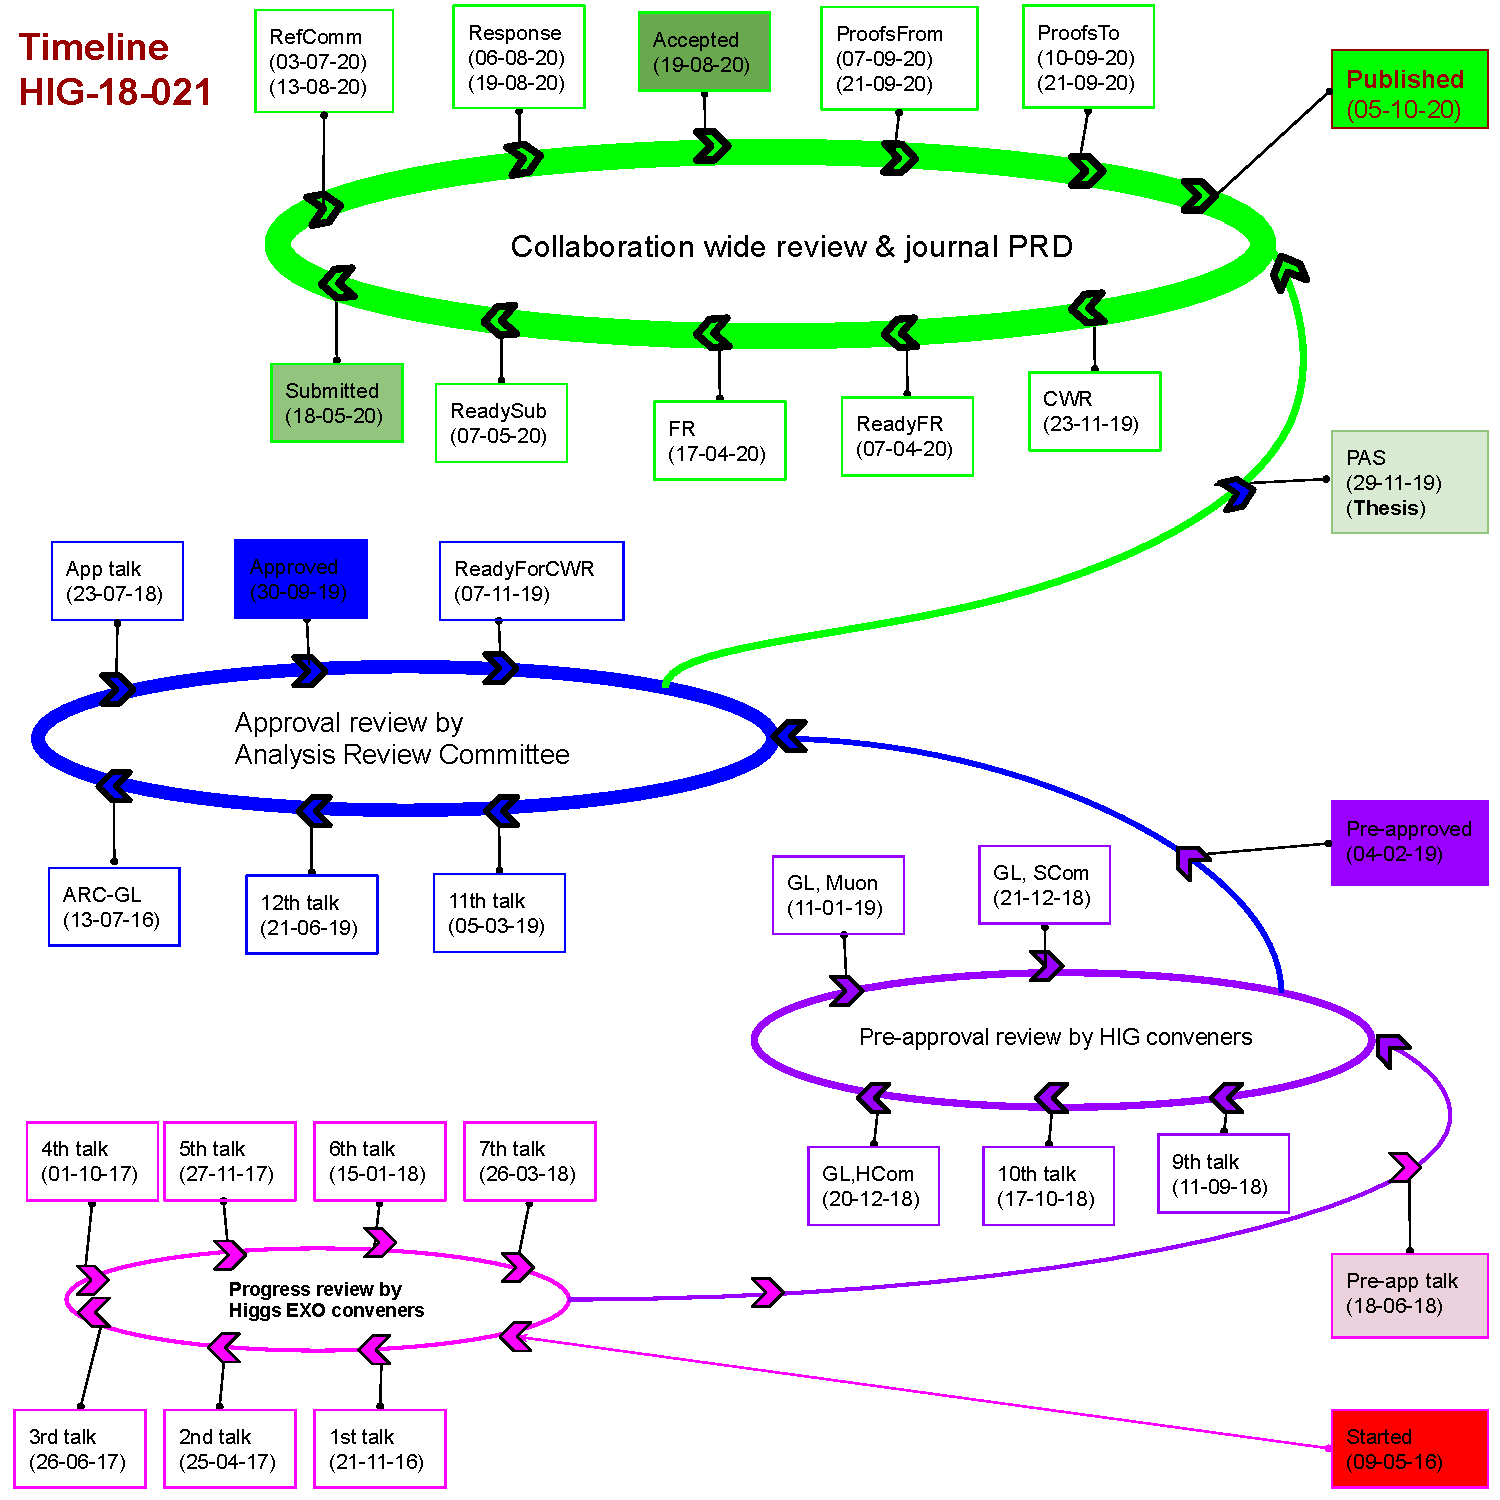
\includegraphics[width=1.0\textwidth]{Image/Timeline_HIG-18-021.pdf}
\caption*{Advancement of the analysis at various review stages. As a
continuation of 8 \TeV analysis, which was published on 29th December 
2015 in the journal JHEP, this analysis at 13 \TeV started in early 2016. 
The first progress report in the Higgs-Exotica meeting was presented on 
21st November 2016. The date on which this analysis was presented 
during pre-approval, approval, collaboration wide review, final reading, 
and publication in the journal PRD is shown in this figure.}
\end{figure}

\newpage

%-------------------------------------
% Introduction
%-------------------------------------
\newpage
\section{Introduction}
\label{s:secIntro}
\section{Introduction}
\label{s:secIntroCMS}
\begin{figure}
  \begin{center}
  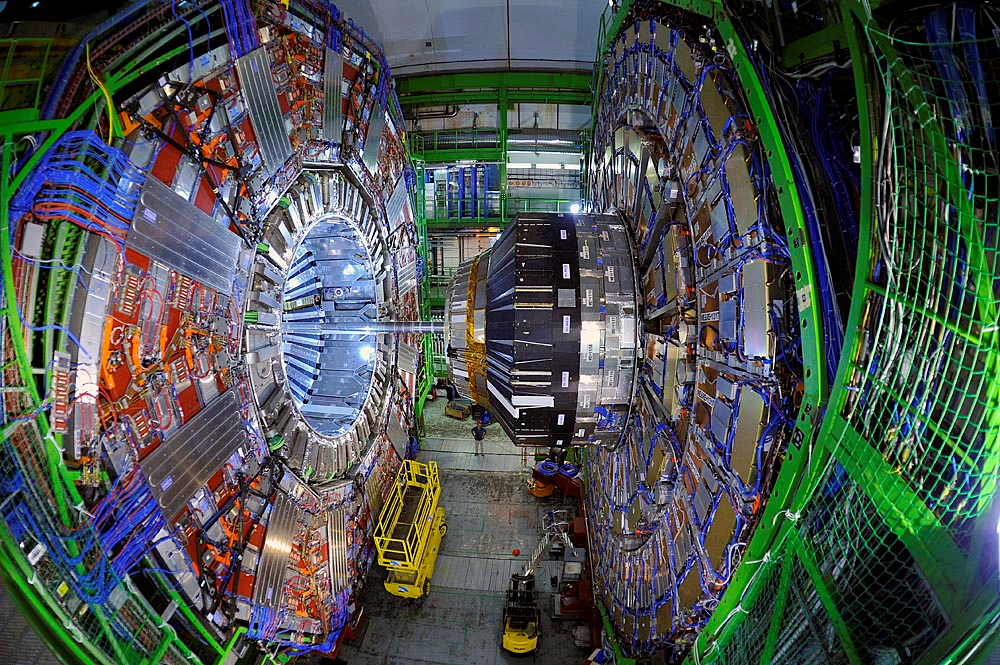
\includegraphics[width=0.90\linewidth]{Experiment/CMS/Image/cms.png}
  \caption{The CMS detector installed in IR5 at the LHC~\cite{Collaboration_2008_CMS}.}
  \label{fig:cms_exp}
  \end{center}
\end{figure}
The Compact Muon Solenoid (CMS) detector is installed in IR5 at the LHC ring. 
CMS is one of the biggest international collaborations involving 43 countries, 
199 institutes, with around 4000 people. The weight of the CMS detector is about 
14000 tonnes (around the weight of 2500 African elephants). Such a huge weight is 
accommodated in a small volume (the shape of CMS is cylindrical with length of 
21.5\unit{m}, and diameter of 15.6\unit{m}). That is why the \dq{compact} word has been 
attached to it. One of the main physics goals of the CMS experiment is to detect \dq{muons} 
as they are produced in most of the Standard Model processes. Of course, other particles 
such as an electron, photon, neutral and charged hadrons are also detected. A huge 
\dq{solenoid} magnet is placed inside the CMS to bend the tracks of charged particles so that 
their momentum can be measured precisely. An image of the CMS experiment is shown
in Figure~\ref{fig:cms_exp}, while various parts of the detectors are shown in Figure
\ref{fig:cms_diag}. The beam axis is along the center of the cylinder. The 
tracker (silicon pixel and strip) is the first sub-detector followed by the 
electromagnetic calorimeter (ECAL), and the hadron calorimeter (HCAL). The
magnetic solenoid is placed outside the HCAL followed by the muon chambers.
The iron yoke provides stand for the muon chambers and contains the magnetic 
flux outside the solenoid. A detailed description of each 
sub-detector is given in the next sections. 

The trajectories of various particles inside the CMS detector are shown in Figure
\ref{fig:cms_track}. The particles are produced at the IP and
move towards various layers of the detector. The charged particles are bent
thanks to the presence of a strong magnetic field inside the solenoid. Outside of it, 
the charged particles are bent in the opposite direction. On the other hand, the neutral particles 
do not bend inside the detector. The particles detected by the CMS experiment are 
muon, electron, charged hadron (e.g. pion), neutral hadron (e.g. neutron), and photon.
\begin{figure}
  \begin{center}
  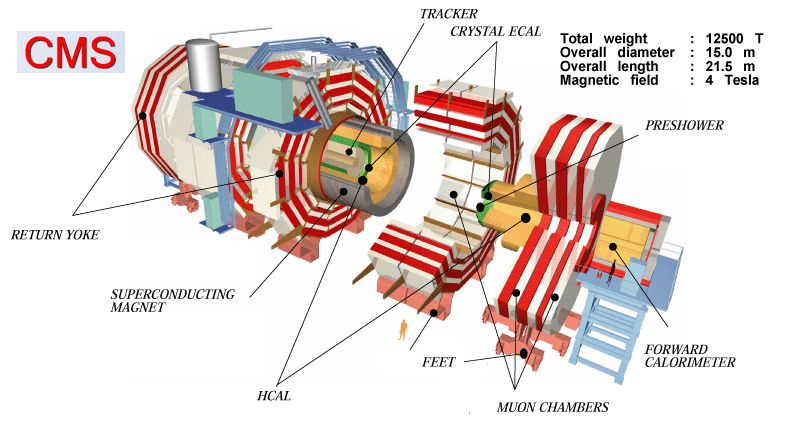
\includegraphics[width=0.90\linewidth]{Experiment/CMS/Image/cmsdiag.png}
	  \caption{Diagram of the CMS detector \cite{cmsDiagram}. Various parts 
	  of the CMS detector are shown starting from tracker to ECAL to HCAL to magnet to 
	  the muon chambers.}
  \label{fig:cms_diag}
  \end{center}
\end{figure}
%Fig\pdfcomment[author={FIG COURTESY}]{http://physics.stackexchange.com/questions/139540/how-detectors-in-particle-colliders-can-differentiate-neutrons-from-antineutrons}}
\begin{figure}
  \begin{center}
  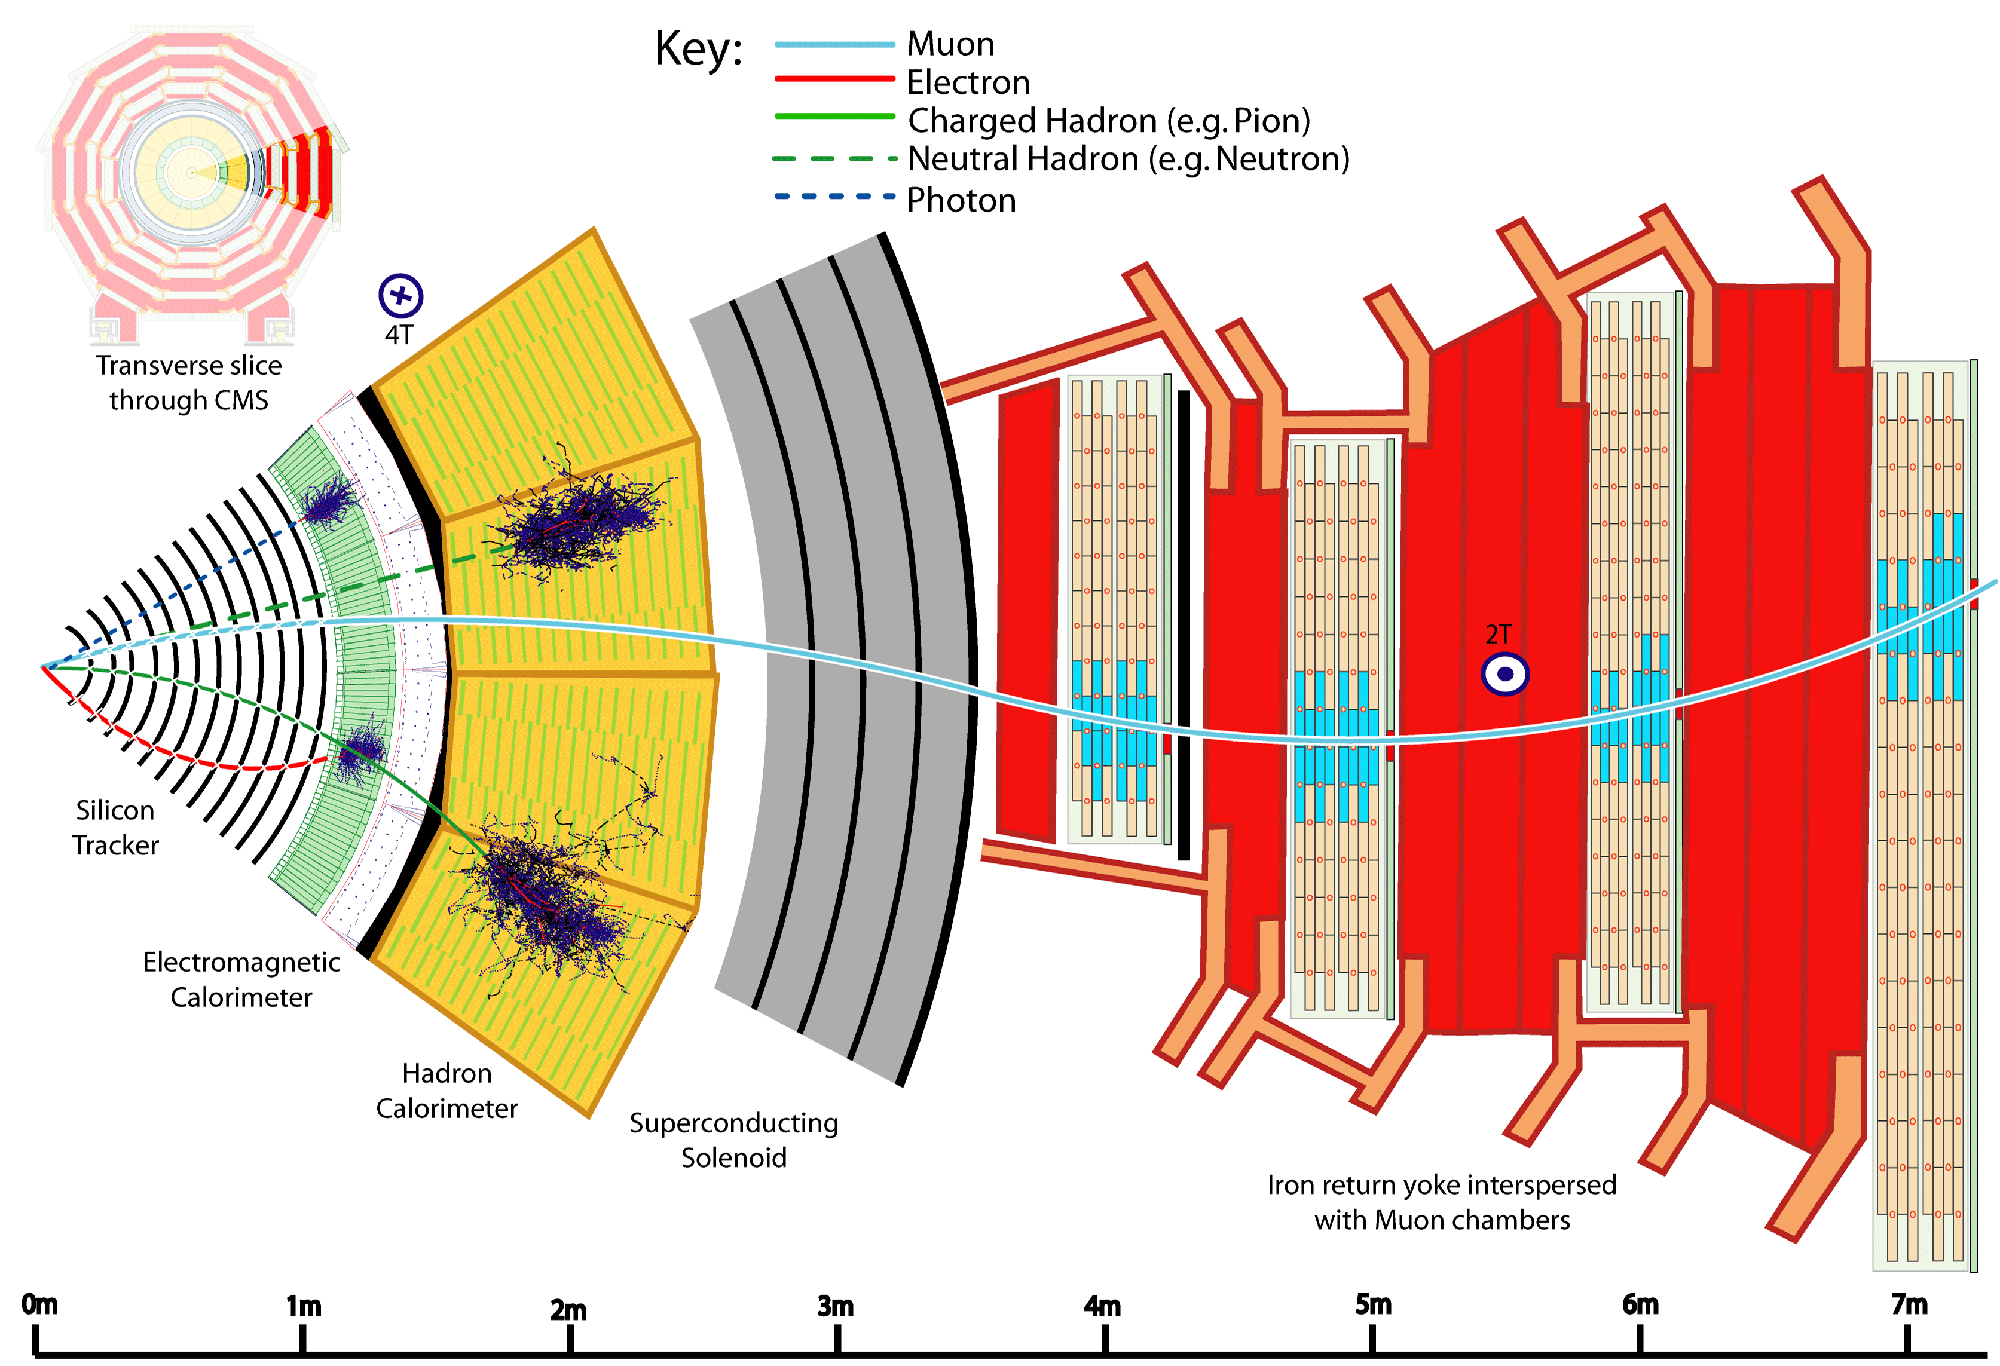
\includegraphics[width=0.90\linewidth]{Experiment/CMS/Image/cmstrack.png}
	  \caption{Trajectories of various particles inside the CMS detector 
	  \cite{Sirunyan:2270046}. The charged particles
	  such as electrons, muons, and charged pions ($\pi^\pm$) are bent inside and 
	  outside the
	  solenoid whereas the neutral particles such as photons and neutral pions ($\pi^0$)
	  traverse without being bent. The silicon tracker is mainly for measuring
	  the momentum of particles whereas the ECAL and HCAL measure the 
	  energy deposits. The electrons and photons deposit their energy inside the 
	  ECAL whereas the hadrons deposit in both ECAL and HCAL. The muons are the
	  only particles that traverses all the way to the muon chambers.}
  \label{fig:cms_track}
  \end{center}
\end{figure}


%-------------------------------------
% Search strategy at 13 TeV
%-------------------------------------
\newpage
\section{Search strategy at 13 TeV}
\label{s:searchStrategy}
 
The search for the charged Higgs boson in the $c\bar{s}$ channel at 13 
\TeV in the CMS experiment adopted a similar strategy as that of the 
previous analysis at 8 \TeV \cite{Khachatryan:2015uua}. An additional 
charm quark tagging have been further exploited to improve sensitivity. 
The invariant mass of the jets originating from charm and strange 
antiquark is taken as the observable for the search of charged Higgs, 
in the low mass region from 80 to 160 \GeV. In the absence of an 
excess in the observed data, a 95\% CL limit is put on the \brThb. The 
charm tagging is extensively used to improve this limit. As shown on 
the right side of the Figure~\ref{fig:feyn_diag_sig}, for the signal 
process, one \PQt quark decays to $H^+ b$ and the other one to 
$W^- \bar{b}$. The $W^+/H^+$ decays hadronically, whereas the $W^-$ 
decays leptonically. As a result, in the final states, there will be 
four jets (2 \PQb jets, 1 \PQc jet, 1 \PQs jet), one lepton (electron 
or muon, $\tau$ is not considered) and missing transverse energy 
attributed to neutrino. In this analysis, we assume that the \brHcs =100\%.
\begin{figure}
\centering
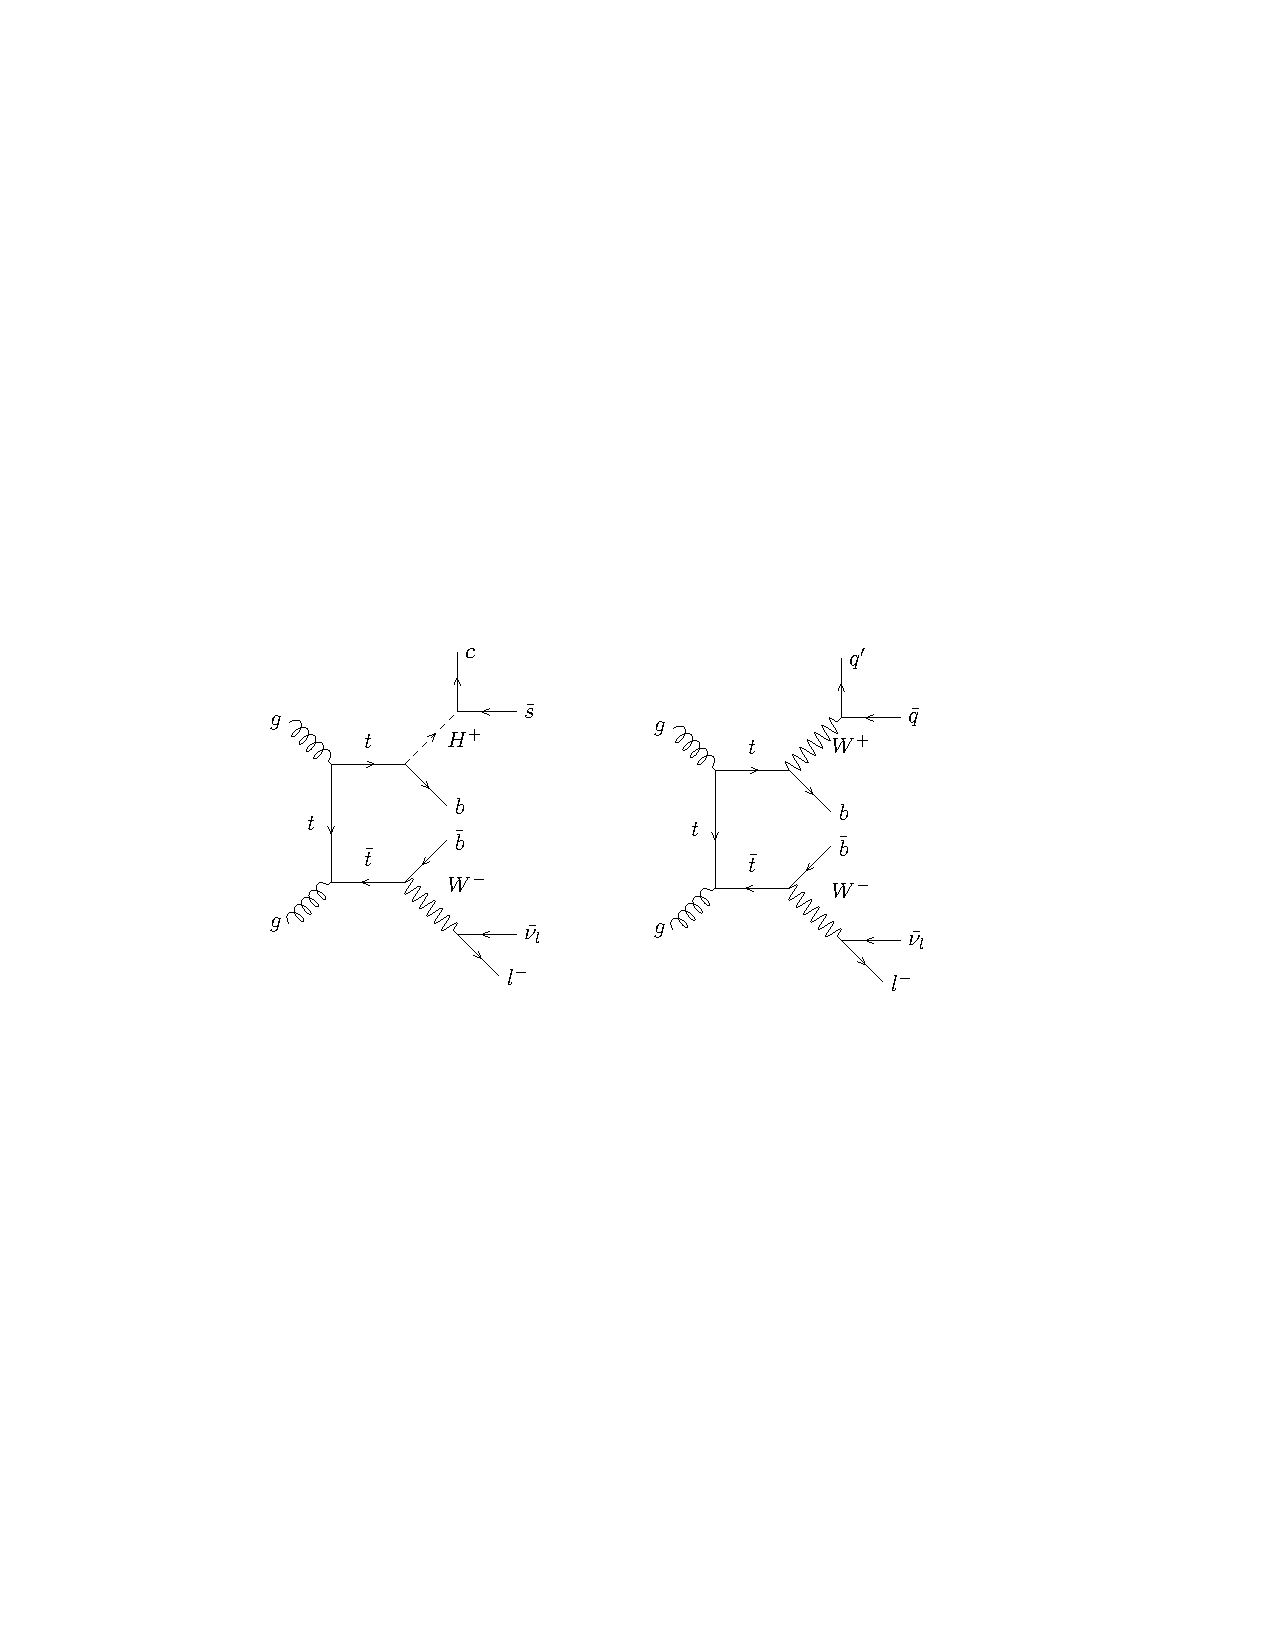
\includegraphics[width=0.75\textwidth]{Image/FeynDiag/feyn_diag_sig.pdf}
\caption{Production of \ttbar from gluon-gluon and quark-quark scattering. 
         The quark-scattering production process has a dominant contribution at 
         Tevatron energies whereas gluon-gluon scattering diagrams are dominant 
         at LHC energies ~\cite{Gerber:2014xea, Fiorini:2012fe}. The SM production
         of \ttbar is shown in (a), (b) and (c). The charged Higgs boson 
         production and its decay are shown in (d), (e) and (f).}
\label{fig:feyn_diag_sig}
\end{figure}

The standard model processes that give same final states (4 jets + 1 
lepton + missing energy) are considered as backgrounds for this 
analysis. The standard model \ttbar production is the most dominant, 
irreducible background process. As shown in the left side of the 
Figure~\ref{fig:feyn_diag_sig}, for SM \ttbar process, one \PQt quark 
decays to the $W^+$ and \PQb quark ($t\rightarrow W^+ b$) and the 
other decays to $W^- \bar{b}$ ($\bar{t}\rightarrow W^-\bar{b}$). The 
SM \ttbar contributes around 94\% of the total backgrounds. Other 
sub-dominant backgrounds that give rise to similar final states are 
single \PQt quark production, QCD multijet, \wjets, \dyjets, and 
vector boson fusion processes. The following background processes are 
considered for the search for charged Higgs. They are ordered in their 
significance of contribution.
\begin{enumerate}
\item $\textbf{SM \ttjets}$: Feynman diagrams 
	for \ttjets production are shown on the left hand side of Figure
	\ref{fig:feyn_diag_sig}. This is the most dominant background channel
	in the search for the signal search region (SR).

\item {\bf{Single \PQt}}: The single \PQt quark production process can also mimic the signal 
	topology. Three different ways, as shown in Figure~\ref{fig:feyn_diag_st}, 
	of production of single top quark considered in this analysis. It is produced through 
	s-channel, t-channel, and tW-channel. In the s-channel and t-channel the initial quarks 
	can be \PQu, \PQd, \PQc and \PQs (4-flavour scheme). However, in the tW-channel, 
	the initial quark is only \PQb quark (5-flavor scheme).
	\begin{figure}
	\begin{center}
	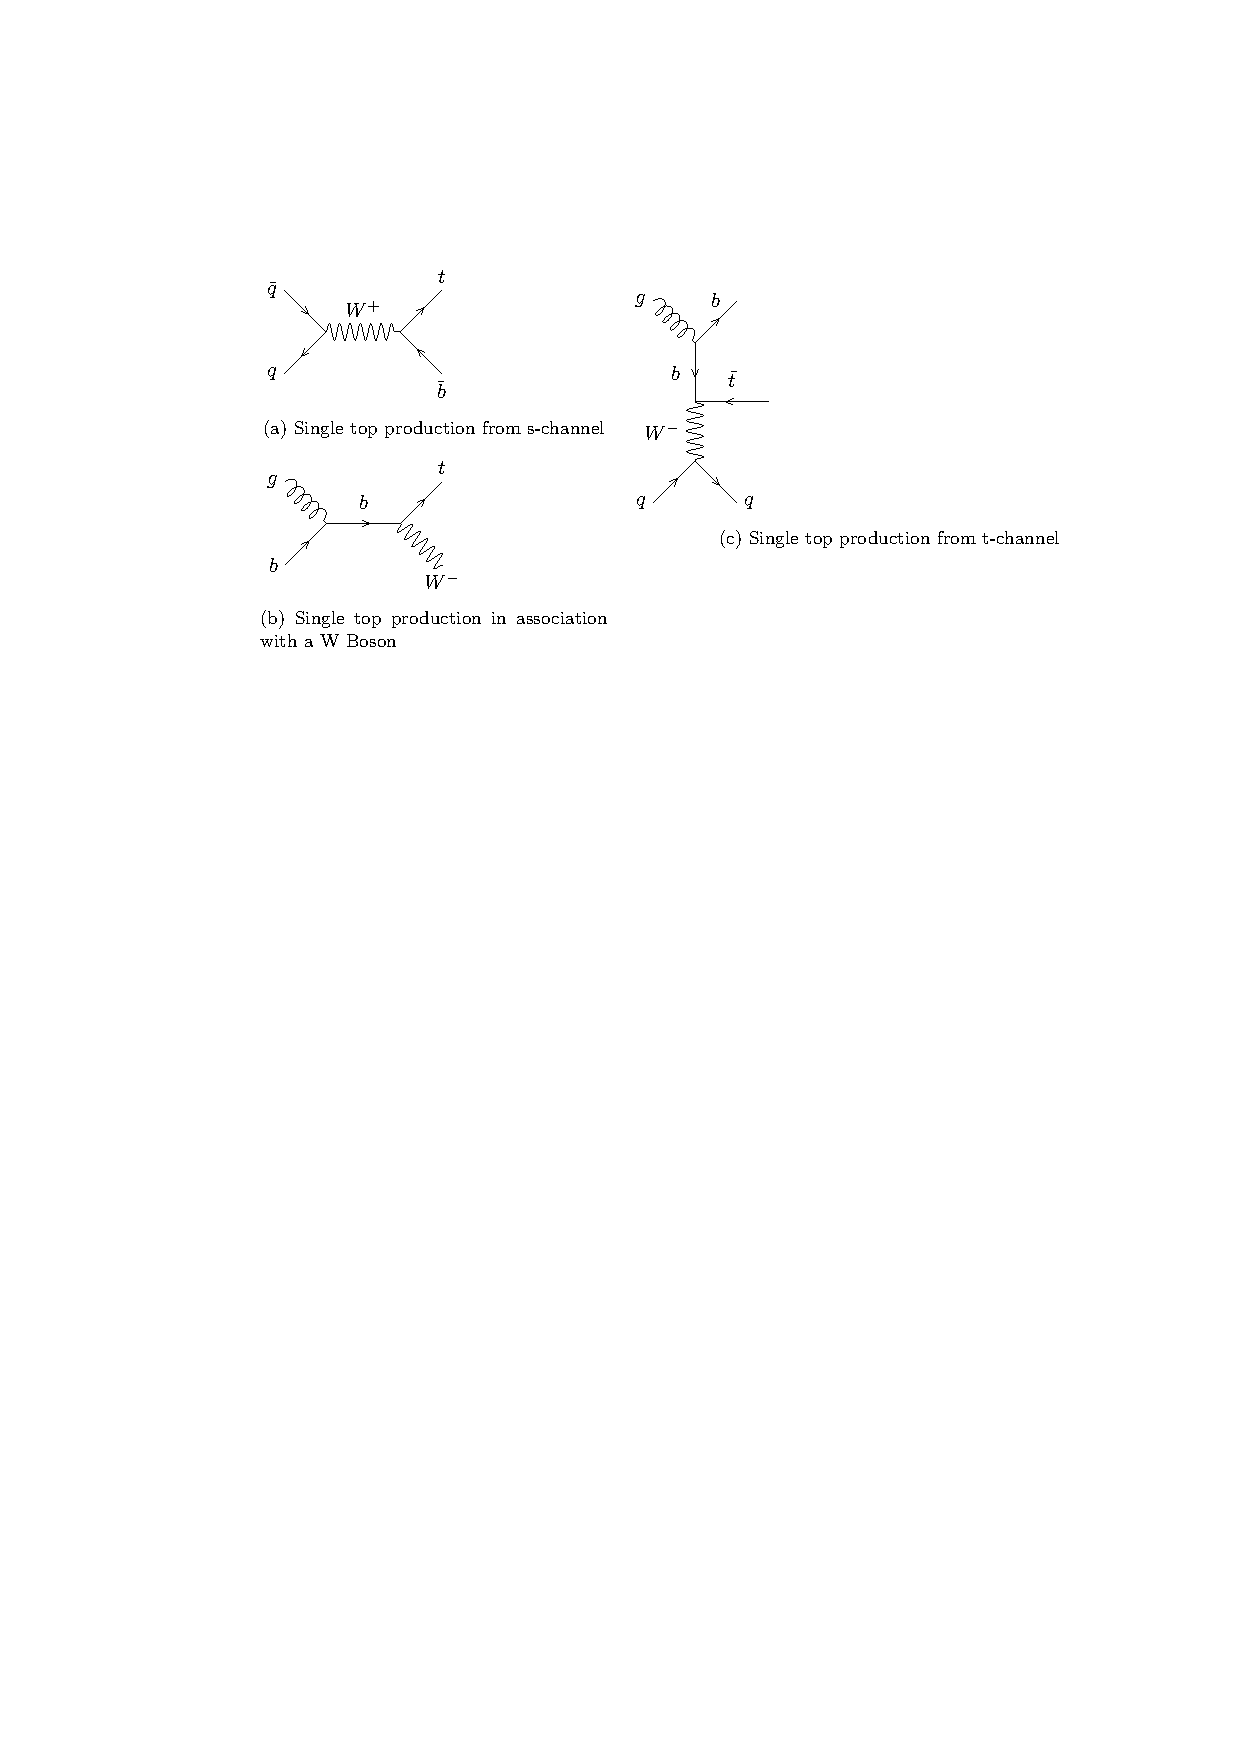
\includegraphics[width=0.75\textwidth]{Image/FeynDiag/feyn_diag_st.pdf}
	\caption{Representative Feynman diagrams for single \PQt quark production processes.}
	\label{fig:feyn_diag_st}
	\end{center}
	\end{figure}

\item {\bf{QCD multijet}}: The QCD multijet events contain only jets 
    at parton level. However, after event reconstruction, they can 
    still have leptons from misidentifications, and \MET due to poor 
    measurement of energy in the detector. Thus these events also 
    mimic the signal topology.

\item {\bf{\wjets}}: In this process, a \PW boson is produced in the 
    proton-proton collisions which subsequently decays leptonically 
    $(\PW^\pm \rightarrow l^+ \nu (l^-\bar{\nu}))$. The following 
    \wjets background process are considered in this analysis:
  	\begin{enumerate}
  	  \item $\PW + \text{jets  }$
  	  \item $\PW + \text{1 jet }$
  	  \item $\PW + \text{2 jets }$
  	  \item $\PW + \text{3 jets }$
  	  \item $\PW + \text{4 jets }$
  	\end{enumerate} 
	The Feynman diagram for these processes are shown in Figure~\ref{fig:feyn_diag_wjet}.
	\begin{figure}
	\begin{center}
	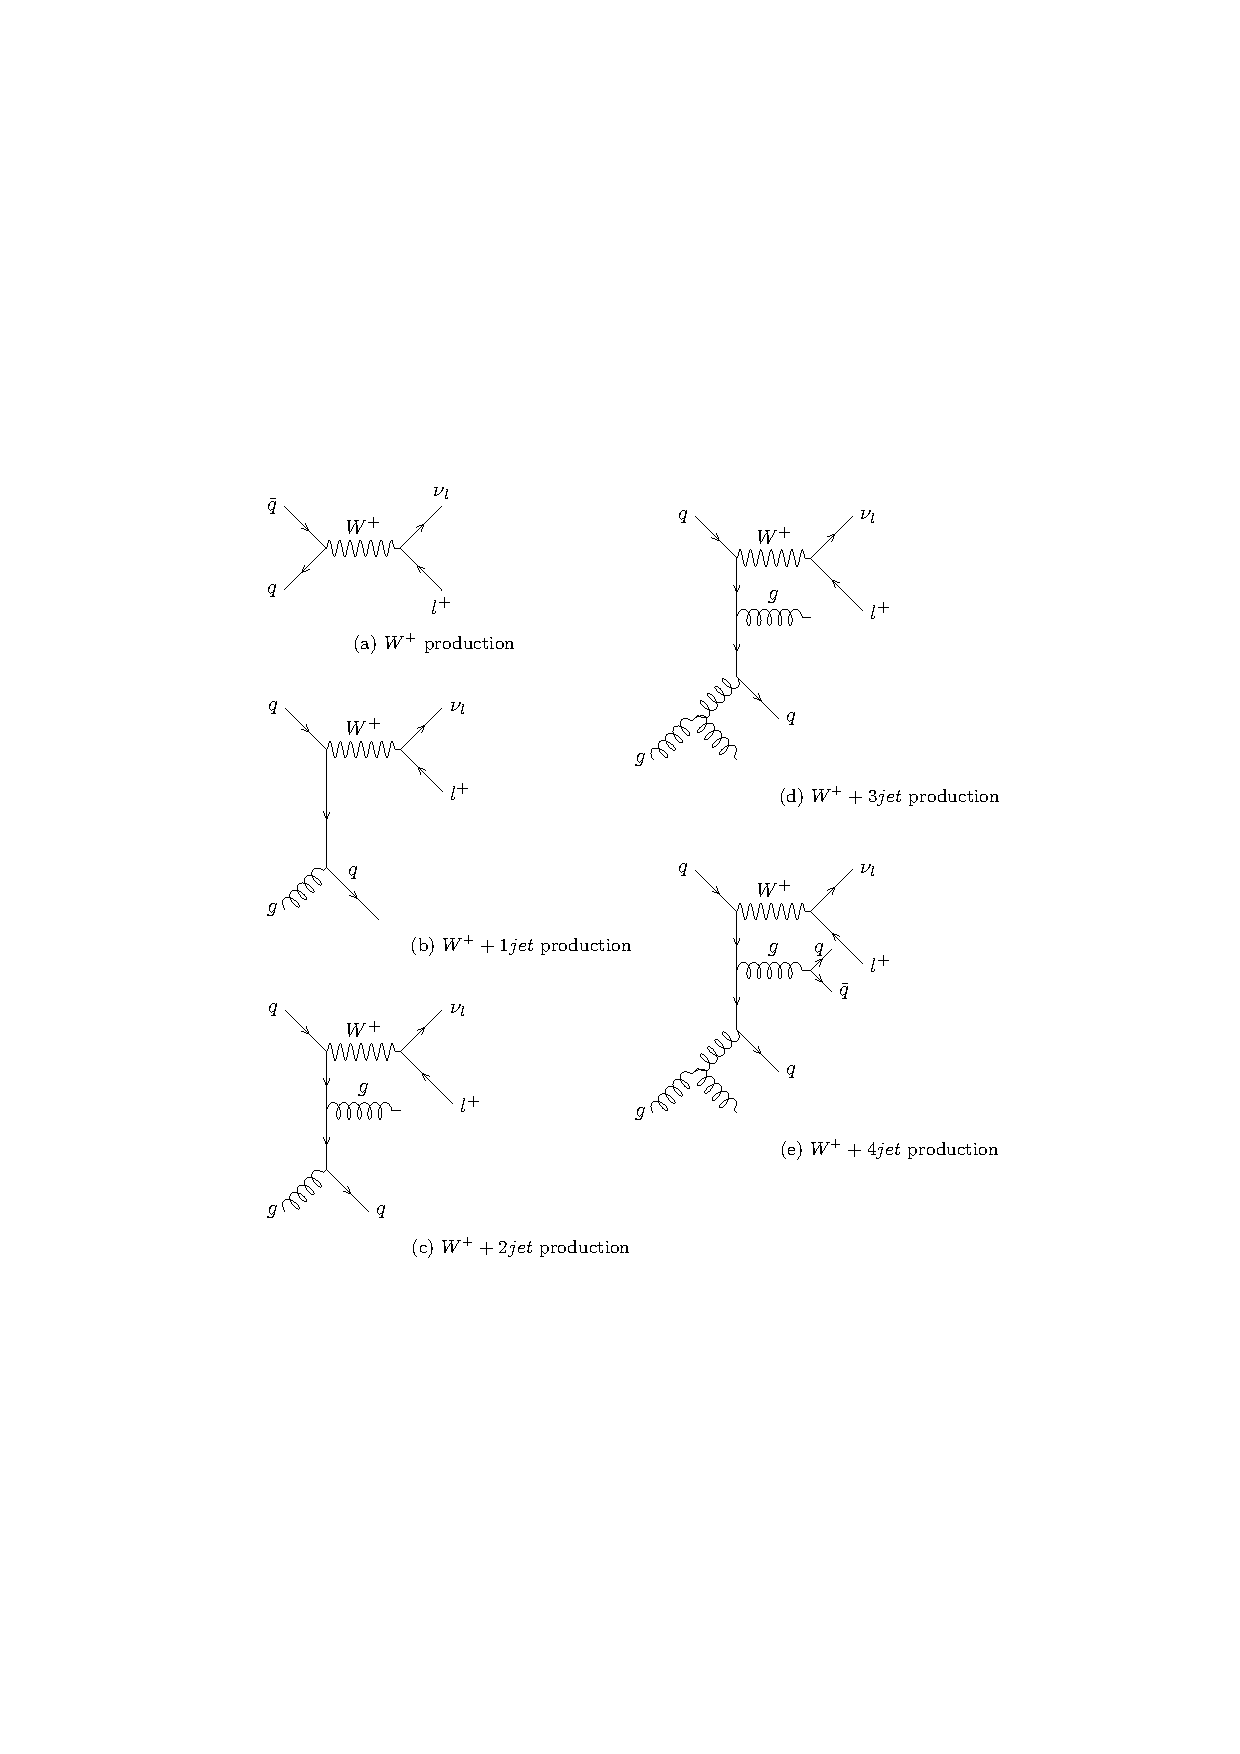
\includegraphics[width=0.75\textwidth]{Image/FeynDiag/feyn_diag_wjet.pdf}
	\caption{Representative Feynman diagrams for $\PW + \text{n jets}$ channel. The 
	\PW boson is produced by quark-quark and quark-gluon scattering 
	along with n jets (n = 0, 1, 2, 3, 4).}
	\label{fig:feyn_diag_wjet}
	\end{center}
	\end{figure}

\item ${\bf{Z/}}$ $\gamma$ ${\bf{+ jets}}$: The Drell-Yan processes in 
    which $Z/\gamma$ are produced along with jets, subsequently 
    decaying to two leptons $(Z/\gamma \rightarrow l^+ l^-)$, have 
    lepton and jets at parton level as shown in 
    Figure~\ref{fig:feyn_diag_dyjet}. However, after the 
    reconstruction, the \MET is also found in the events due to the 
    poor measurement of energy in the detector.
	\begin{enumerate}
  	\item $Z/\gamma +\text{ jets   }$
  	\item $Z/\gamma +\text{ 1 jet  }$
  	\item $Z/\gamma +\text{ 2 jets }$
  	\item $Z/\gamma +\text{ 3 jets }$
  	\item $Z/\gamma +\text{ 4 jets }$
  	\end{enumerate}
	\begin{figure}
	\begin{center}
	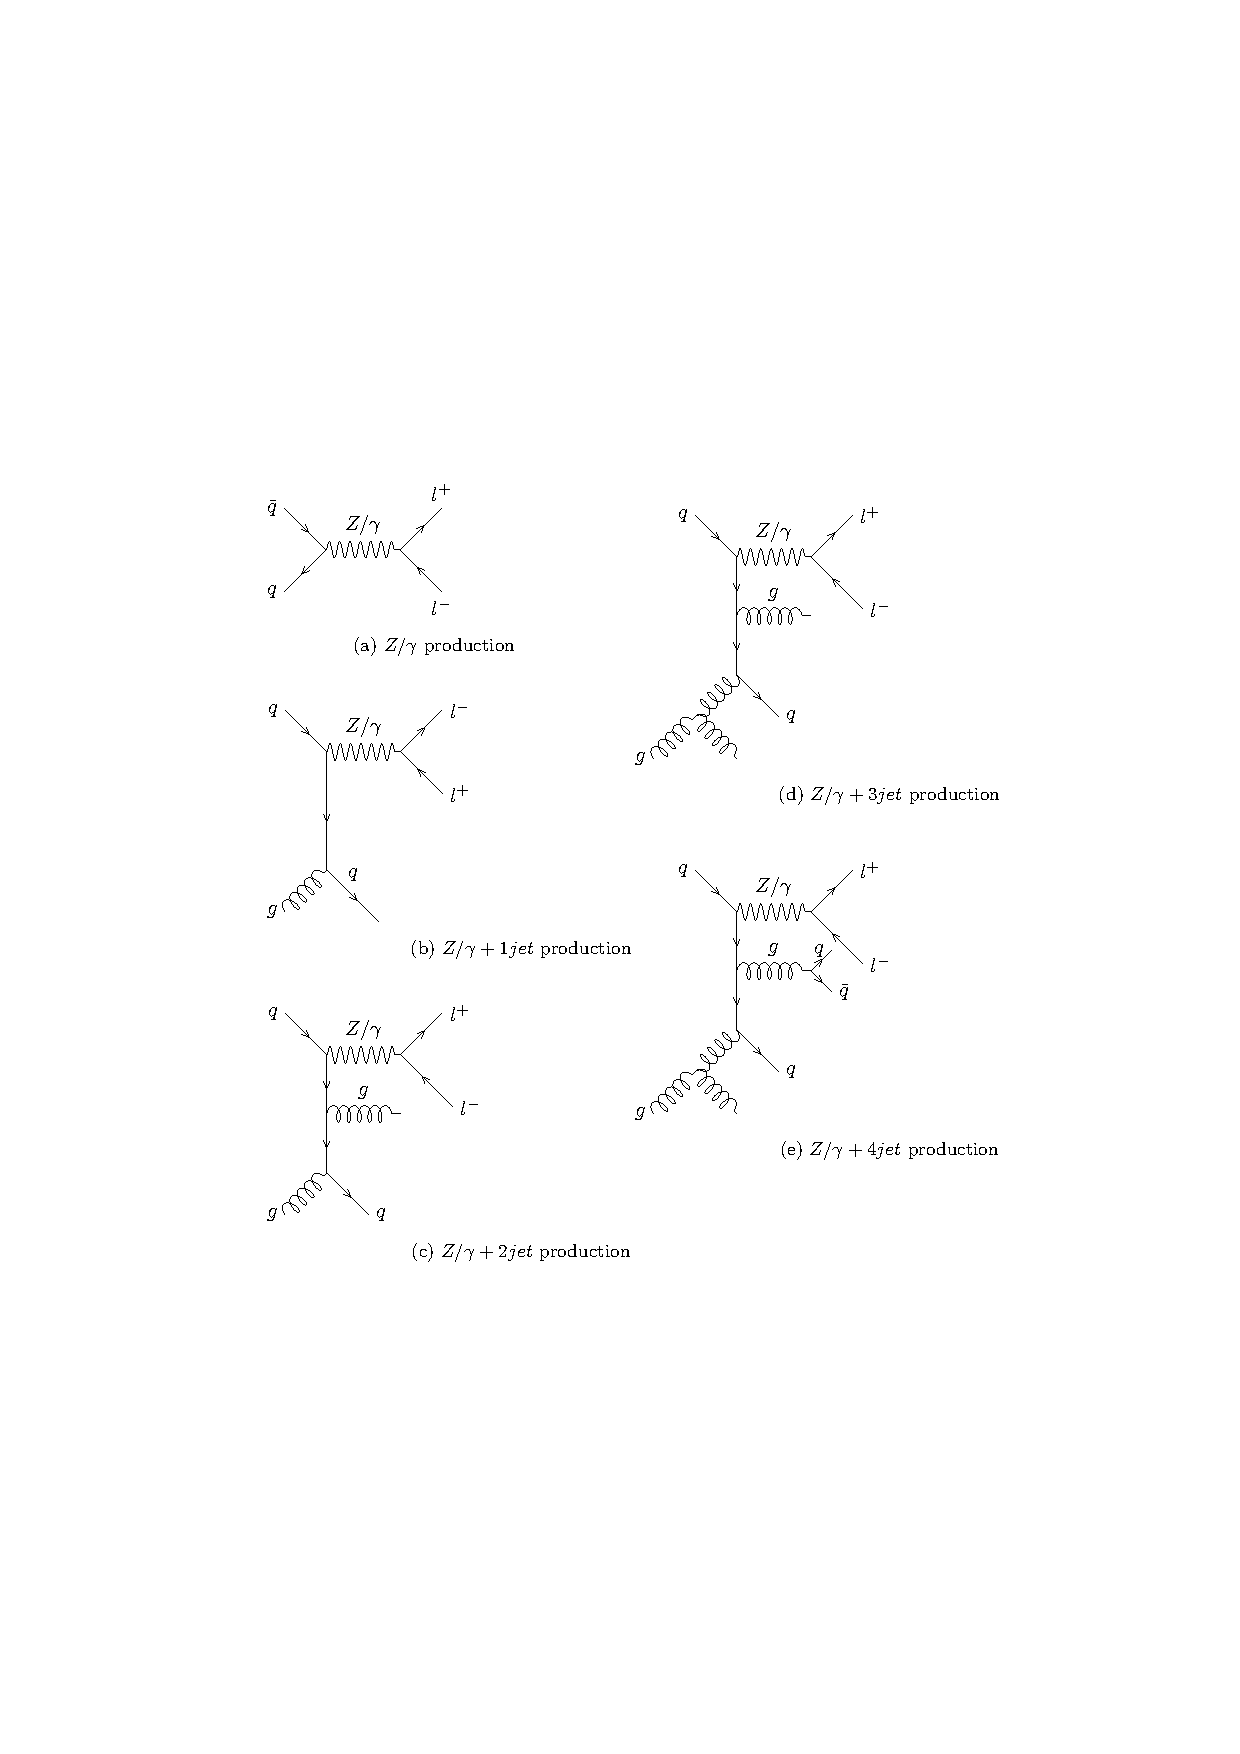
\includegraphics[width=0.75\textwidth]{Image/FeynDiag/feyn_diag_dyjet.pdf}
	\caption{Representative Feynman diagrams for $ Z/\gamma + \text{n jets}$ channel. 
	The $Z/\gamma$ is produced by quark-quark and quark-gluon scattering 
	along with n jets (n = 0, 1, 2, 3, 4).}
	\label{fig:feyn_diag_dyjet}
	\end{center}
	\end{figure}

\item {\bf{VV}}: Vector boson fusion processes are the smallest 
    background in the signal search region. The fusion happens via 
    tri-linear coupling between the $W^\pm$ and \PZ. The \PZ boson 
    further decays to $l^+l^-$. The VV process has three 
    sub-categories: WW, WZ, and ZZ. The vector Boson fusion process 
    is shown in Figure~\ref{fig:feyn_diag_vv}.
\begin{figure}
\begin{center}
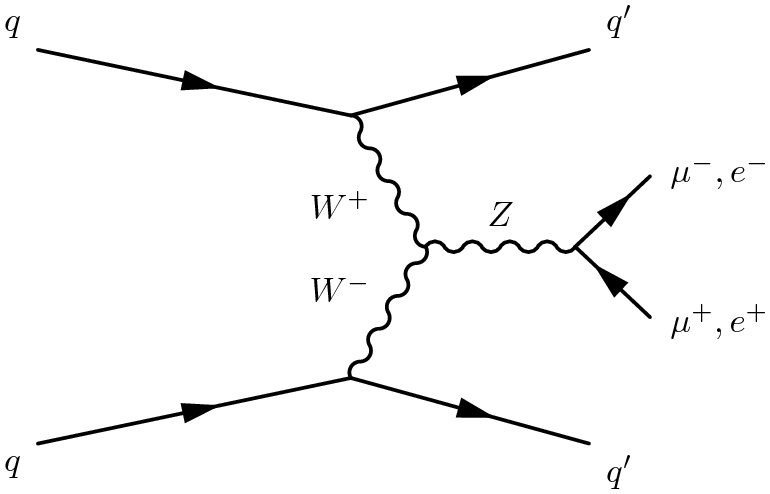
\includegraphics[width=0.40\textwidth]{Image/FeynDiag/feyn_diag_vv.png}
\caption{Representative Feynman diagram for vector Boson fusion process.}
\label{fig:feyn_diag_vv}
\end{center}
\end{figure}
\end{enumerate}



%-------------------------------------
% MC and Data Samples
%-------------------------------------
\newpage
\section{Data and Simulated Samples}
\label{s:secDataMC}

%%%%%%%%%%%%%%%%%%%%%%%%%%%%%%%%%%%%%%%%%%%%%%%%%%%%%%%%
\subsection{Data Samples}
The reconstructed data is broadly divided into different event topologies. Only those 
datasets matching with event topology under consideration are used for the analysis. 
Such approach help in optimising the computing resources.
The single muon and single electron data sample used for this analysis are shown in
Table (\ref{tab:dataSample}). The data was collected in 2016 corresponding to Run number 
273158 to 284044. To select good quality data, where most of the sub-detectors of the CMS 
operates in a normal condition; the following lumi mask, as recommended by the PdMV group is applied:
\verb|Cert_271036-284044_13TeV_23Sep2016ReReco_Collisions16_JSON.txt|. The integrated luminosity
after applying the mask reduces marginally from 37.0\fbinv to
35.9\fbinv. The luminosity is calculated using the Command (\ref{cmd:lumiCalc}). 
The global tag \verb|80X_dataRun2_2016SeptRepro_v7| is used to process the {\em MINIAOD}
data in the \verb|CMSSW_8_0_28| for the production of the {\em ntuples}. The same version
of the \verb|CMSSW| is used to produce {\em ntuples} for data, background, and signal samples.

\begin{table}
\centering
    \caption{Muon and Electron data samples recorded in 2016 with an integrated luminosity 35.9
    \fbinv. The re-reco campaign was used for Run B to Run G. For Run H, prompt reconstructions were used. 
    The luminosity is calculated using {\bf{brilcalc}} tool. Where M = \/MINIAOD.} 
\label{tab:dataSample}
\begin{adjustbox}{max width=\textwidth}
\begin{tabular}{cccc} \hline\hline                                                                                                                  
    {\bf{Dataset}} & {\bf{$\boldmath{L}_{int}$ (\fbinv)}} & {\bf{Run}} & {\bf{Events}}
    \\\hline\hline
 \verb|/SingleMuon/Run2016B-03Feb2017_ver2-v2/M|    & 5.78 & 273158-275376  & 154054252  \\[0.1cm]
 \verb|/SingleMuon/Run2016C-03Feb2017-v1/M|         & 2.57 & 275657-276283  & 64718679   \\[0.1cm]
 \verb|/SingleMuon/Run2016D-03Feb2017-v1/M|         & 4.25 & 276315-276811  & 96657799  \\[0.1cm]
 \verb|/SingleMuon/Run2016E-03Feb2017-v1/M|         & 4.01 & 276831-277420  & 87362752   \\[0.1cm]
 \verb|/SingleMuon/Run2016F-03Feb2017-v1/M|         & 3.10 & 277981-278808  & 65047318   \\[0.1cm]
 \verb|/SingleMuon/Run2016G-03Feb2017-v1/M|         & 7.54 & 278820-280385  & 147945745  \\[0.1cm]
 \verb|/SingleMuon/Run2016H-03Feb2017_ver2-v1/M|    & 8.40 & 281613-284035  & 166591136  \\[0.1cm]
 \verb|/SingleMuon/Run2016H-03Feb2017_ver3-v1/M|    & 0.21 & 284036-284044  & 4389914    \\\hline
     {\bf{Total}}                                    & {\bf{35.86}} & {\bf{273158-284044}}  &
     {\bf{786767595}}    \\[0.1cm]\hline                                                   

 \verb|/SingleElectron/Run2016B-03Feb2017_ver2-v2/M|    & 5.78 & 273158-275376  & 237366108  \\[0.1cm]
 \verb|/SingleElectron/Run2016C-03Feb2017-v1/M|         & 2.57 & 275657-276283  & 91591087   \\[0.1cm]
 \verb|/SingleElectron/Run2016D-03Feb2017-v1/M|         & 4.25 & 276315-276811  & 146495223  \\[0.1cm]
 \verb|/SingleElectron/Run2016E-03Feb2017-v1/M|         & 4.01 & 276831-277420  & 113169852  \\[0.1cm]
 \verb|/SingleElectron/Run2016F-03Feb2017-v1/M|         & 3.10 & 277981-278808  & 70143321   \\[0.1cm]
 \verb|/SingleElectron/Run2016G-03Feb2017-v1/M|         & 7.54 & 278820-280385  & 152098617  \\[0.1cm]
 \verb|/SingleElectron/Run2016H-03Feb2017_ver2-v1/M|    & 8.40 & 281613-284035  & 123900510  \\[0.1cm]
 \verb|/SingleElectron/Run2016H-03Feb2017_ver3-v1/M|    & 0.21 & 284036-284044  & 3189661    \\\hline
   {\bf{Total}}                                          & {\bf{35.86}} & {\bf{273158-284044}}  & {\bf{937954379}}    \\\hline
 \end{tabular}          
\end{adjustbox}









\end{table}

\subsection{Simulated Samples}
The centrally produced official simulated samples are used in this analysis. 
Production of most of the samples (except 
\verb|QCD_Pt-15to20_EMEnriched|) started with campaign 
\verb|RunIISummer16MiniAODv2| and final reconstruction was done with 
campaign \verb|PUMoriond17| using Global Tag \\ 
\verb|80X_mcRun2_asymptotic_2016_TrancheIV_v6|. 
The simulated samples used in this analysis are shown in Table (\ref{tab:mcSample}) 
with corresponding cross-section and number of simulated events. 
The k-factor is the ratio of cross-sections from next-to-leading-order 
and leading-order, k$_\text{f} =\sigma_{\text{NLO}}/\sigma_{\text{LO}}$.

The signal and background simulated samples are generated using \MGvATNLO~\cite{Alwall:2011uj, Alwall:2014hca}
as well as \POWHEG~\cite{Frixione:2007vw, Nason:2004rx, Alioli:2010xd} generators at parton level. 
These parton level events are hadronised using \PYTHIA~\cite{Sjostrand:2006za, Sjostrand:2007gs}. 
The hadronised events were tuned using  CUETP8M1~\cite{CMS-PAS-TOP-16-021} which are then passed
through \GEANTfour~\cite{Agostinelli:2002hh} for detector simulation. Finally, the events are
reconstructed after complete detector simulation. In summary, the 
following steps are followed to produce simulated samples for a single process:
\begin{enumerate}
    \item {\bf{GEN-SIM}}: 
        \begin{itemize}
            \item GEN: Physics process generation. 
            \item SIM: Detector simulation.
        \end{itemize}
    \item {\bf{RECO}}: 
        \begin{itemize}
            \item DIGIPREMIX\_S2: \\
                \verb|https://twiki.cern.ch/twiki/bin/view/CMSPublic/SWGuideSimulation|, 
            \item DATAMIX: \\\verb|https://twiki.cern.ch/twiki/bin/view/CMSPublic/SWGuideSimulation|,
            \item L1: L1 trigger emulation,
            \item DIGI2RAW: Conversion of the digitised data format to raw data format, 
            \item HLT: Applying high level trigger,
            \item RAW2DIGI: Conversion of the raw data format to DIGI data format,
            \item RECO: Reconstruction of physics object,
            \item EI: High-level reconstruction step used in validation.
        \end{itemize}
    \item {\bf{MINIAOD}}: Re-reconstruction of physics object.
\end{enumerate}

The \ttjets channel is the most significant irreducible background for this analysis. It
contributes around 94\% of the total backgrounds in the signal region. The parton level events 
for \ttjets samples of Table~\ref{tab:mcSample} are generated using 
\POWHEG~\cite{Frixione:2007vw, Nason:2004rx, Alioli:2010xd} at next-to-leading (NLO) order. The 
\verb|NNPDF30_nlo_as_0118| ~\cite{Ball:2014uwa} parton distribution function (PDF) was used 
for this purpose. The partonic events were then hadronised using 
\PYTHIA~\cite{Sjostrand:2006za, Sjostrand:2007gs}. To simulate this channel at higher orders and 
to take care of non-perturbative effects, \ttjets samples were tuned with 
CUETP8M1~\cite{CMS-PAS-TOP-16-021}. The NNLO cross section for \ttjets process is estimated to be 
$831.76 \pm^{20}_{29}(\text{scale}) \pm 35 (\text{PDF} + \alpha_s)$ pb \cite{Beneke:2011mq}. 

Initially, the \ttjets sample was simulated using MadGraph generator (\\ 
\verb|/TTJets_TuneCUETP8M1_13TeV-madgraphMLM-pythia8/year+M|, where \verb|year| and \verb|M| 
are defined in Table (\ref{tab:mcSample}). However, MadGraph-MLM sample was found to be 
improperly modeled for high jet multiplicity due to which there was a surplus of 5\% (4\%) 
simulated events w.r.t. observed data for muon (electron) + jets channel in the signal region as 
shown in Figure~\ref{fig:MGvsPG}. In view of this, the POWHEG \ttjets sample is used in this analysis.
Comparison of POWHEG and Madgraph \ttjets sample is described in Appendix~\ref{a:appendMGvsPG}.

Single \PQt quark samples are shown in Table~\ref{tab:mcSample}, where a \PQt quark is produced with 
jets in \PQt-channel (\verb|ST_t|), \PQs-channel (\verb|ST_s|), and \PQt\PW-channel (\verb|ST_tW|). The
\verb|ST_tW| and \verb|ST_t| samples are produced using \POWHEG + \PYTHIA and CUETP8M1, where \verb|ST_tW| has 
5-flavor scheme whereas \verb|ST_t|, has 4-flavor scheme and further, the \PQt quark decays 
inclusively. The \verb|ST_s| are generated using \MGvATNLO~\cite{Alwall:2014hca} in the 4-flavor 
scheme and was hadronised using \PYTHIA. The NLO cross section for single \PQt process 
\cite{Aliev:2010zk, Kant:2014oha} are shown in Table~\ref{tab:mcSample}.

The inclusive \wjets and \dyjets samples were generated using \MGvATNLO and are hadronised using 
\PYTHIA. The MLM~\cite{ Alwall:2007fs} technique was used to take care of double counting. There
are exclusive \PW + n jets and $\PZ/\PGg$ + n jets samples available for n = 1, 2, 3, 4. 
The inclusive (\wjets and \dyjets) and exclusive ($\PW/\PZ/\PGg$ + n jets) samples have our event 
topology \ie 4 jets + 1 lepton + \MET. Therefore, the inclusive and exclusive samples are added 
appropriately to have more statistics. To avoid double counting, an 
event weight based on luminosity and number of particles (NUP) 
including incoming, intermediate, and outgoing at generator level is 
applied to each sample. After that, the final event yields from each of
them are added linearly. The event weight for NUP = 5, 6, 7, 8, and $\geq$9 is
 $L_{data}/L_{\wjets}$, $L_{data}/(L_{\wjets} + L_{\PW + \text{1 jet}})$, 
 $L_{data}/(L_{\wjets} + L_{\PW + \text{2 jet}})$, 
 $L_{data}/(L_{\wjets} + L_{\PW + \text{3 jet}})$,
 $L_{data}/(L_{\wjets} + L_{\PW + \text{4 jet}})$, respectively.
 Where, for example, $L_{\wjets}$ is the generated luminosity (number 
 of events divided by the cross section) of \wjets sample. A similar 
 procedure is followed to add $\PZ/\PGg$ + n jets with \dyjets. However,
 the NUP variable does not count the intermediate photon as the status
 of photon is not displayed in the LHE event file. Hence it is
 incremented by 1 when a \PZ boson is not the intermediate particle.
 The NLO cross section for these processes are shown in Table~\ref{tab:mcSample}.

The vector boson fusion process (WW, WZ, and ZZ) samples are generated and hadronised 
using \PYTHIA and are tuned using CUETP8M1. The NLO cross section for these samples are shown 
in Table~\ref{tab:mcSample}.

The muon (electron) enriched QCD multijet samples are used for \mujets (\ejets) channel. These 
samples are generated using \PYTHIA and CUETP8M1. After multiplying with filter efficiency, the 
NLO cross sections are shown in Table~\ref{tab:mcSample}. From this table, it can be seen that the 
luminosity for these samples are significantly 
smaller as compared to the observed luminosity and therefore, a data-driven approach is used to 
make more precise estimation of QCD multijet background.

The charged Higgs signal samples were generated using \MGvATNLO, and hadronized using \PYTHIA. The 
signal sample for several mass points in the range of 80 to 160 \GeV (80, 90, 100, 120, 140, 150, 
155, 160) are generated for the search for charged Higgs. The cross section 
for the signal is 831.76$\times$ 0.2132 pb, where 831.76 \unit{pb} is the inclusive 
(fully-hadronic, fully-leptonic, semi-leptonic) \ttjets production cross section and factor 
0.2132 is the branching fraction of $W^-\to l^- \bar{\nu_l}$ (where $l = \mu, e$, $\tau$ is not 
considered in this analysis) \cite{Beringer:1900zz}. The factor 0.2132 is multiplied because \ttbar decays 
semi-leptonically ($(t\to H^+ b, H^+\to c\bar{s}), (\bar{t}\to W^-\bar{b}, W^- \to l^-\bar{\nu_l})$), 
where $l = \mu, e$ in the charged Higgs signal samples. Furthermore, the signal events are scaled by 
the maximum observed upper limit obtained at 8 \TeV. The upper observed limit on \brThb is 6.5\% for
the $m_{H+}$ = 90 \GeV\cite{Khachatryan:2015uua}. Therefore, the signal samples are scaled by a factor 
$2\times 0.065\times (1-0.065) = 0.12155$ in every plot and table except in the data cards used for 
limit computation. 
\begin{table}
\caption{Signal and background simulated samples. Where \\  
\small{
run = { \em RunIISummer16MiniAODv2-PUMoriond17\_80X\_mcRun2\_asymptotic\_2016\_TrancheIV\_v6}, \\
run2= { \em RunIISpring16MiniAODv2-FlatPU8to37HcalNZSRAW\_withHLT\_80X\_mcRun2\_asymptotic\_v14-v1},\\
M = /MINIAODSIM, yext1\_v2 = { \em run\_ext1-v2, yext1\_v1 = run\_ext1-v1},year = run-v1.
}
}
\label{tab:mcSample}
\centering

\begin{adjustbox}{max width=\textwidth}
\begin{tabular}{cccc} \hline\hline
    {\bf{MC Dataset}} & {\bf{$\sigma$}} (pb)(Order) &{\bf{$k_f$}}& {\bf{Events}}\\\hline\hline
    \verb|/TT_TuneCUETP8M2T4_13TeV-powheg-pythia8/+year+M|     
    &$831.76^{+20}_{-29} \pm 35$(NNLO) & --- & 77081156 \\ [0.1cm] 
    \verb|/ST_tW_antitop_5f_inclusiveDecays_13TeV-powheg| \\ 
    \verb|-pythia8_TuneCUETP8M1/+yext1_v1+M|  
    &$71.7 \pm 1.80 \pm 3.40$(NLO) & --- &  6933094   \\[0.1cm]
    \verb|/ST_t-channel_antitop_4f_inclusiveDecays_13TeV-powhegV2|\\
    \verb|-madspin-pythia8_TuneCUETP8M1/+year+M|  
    &$80.95^{+5.8}_{-5.2} \pm 0.16$(NLO) & ---  & 38811017  \\ [0.1cm]
    \verb|/ST_s-channel_4f_InclusiveDecays_13TeV-amcatnlo-pythia8/+year+M|  
    &$10.32^{+0.6}_{0.5} \pm 0.01$(NLO) & ---  & 2989199  \\[0.1cm] \hline
    
    \verb|/WJetsToLNu_TuneCUETP8M1_13TeV-madgraphMLM-pythia8/+year+M|       
    &$50690 \pm 389.1$(LO) & 1.21  & 29181900  \\[0.1cm]
    \verb|/W1JetsToLNu_TuneCUETP8M1_13TeV-madgraphMLM-pythia8/+year+M|   
    &$9493 \pm 25.52$(LO)      & 1.21  & 44813600  \\[0.1cm]
    \verb|/W2JetsToLNu_TuneCUETP8M1_13TeV-madgraphMLM-pythia8/+year+M|      
    &$3120 \pm 78.5$(LO)   & 1.21  & 29878415  \\[0.1cm]
    \verb|/W3JetsToLNu_TuneCUETP8M1_13TeV-madgraphMLM-pythia8/+year+M|      
    &$942.3 \pm 36.8$(LO)  & 1.21  & 19798117  \\[0.1cm]
    \verb|/W4JetsToLNu_TuneCUETP8M1_13TeV-madgraphMLM-pythia8/+year+M|      
    &$524.2 \pm 23.6$(LO)  & 1.21  & 9170576  \\[0.1cm]\hline

    \verb|/DYJetsToLL_M-50_TuneCUETP8M1_13TeV-madgraphMLM-pythia8/+yext1_v2+M| 
    &$4895 \pm 41$(LO)    & 1.17  & 48103700  \\[0.1cm]
    \verb|/DY1JetsToLL_M-50_TuneCUETP8M1_13TeV-madgraphMLM-pythia8/+year+M|
    &$1016 \pm 16.8$(LO)  & 1.17  & 62079400  \\[0.1cm]
    \verb|/DY2JetsToLL_M-50_TuneCUETP8M1_13TeV-madgraphMLM-pythia8/+year+M|     
    &$331.3\pm 8.5$(LO)   & 1.17  & 19970551  \\[0.1cm]
    \verb|/DY3JetsToLL_M-50_TuneCUETP8M1_13TeV-madgraphMLM-pythia8/+year+M|     
    &$96.6 \pm 3.9$(LO)   & 1.17  & 5856110  \\[0.1cm]
    \verb|/DY4JetsToLL_M-50_TuneCUETP8M1_13TeV-madgraphMLM-pythia8/+year+M|     
    &$51.4 \pm 2.5$(LO)   & 1.17  & 4197868  \\[0.1cm] \hline

    \verb|/WW_TuneCUETP8M1_13TeV-pythia8/+year+M|  
    &$118.7^{+2.5}_{-2.2}$(NNLO) & ---   & 994012  \\[0.1cm] 
    \verb|/WZ_TuneCUETP8M1_13TeV-pythia8/+year+M|  
    &$46.74^{+1.9}_{1.5}$(NLO)  & ---  & 1000000 \\[0.1cm] 
    \verb|/ZZ_TuneCUETP8M1_13TeV-pythia8/+year+M|  
    &$17.72^{0.6}_{0.4}$(NLO)  & ---  & 990064  \\[0.1cm] \hline
 \verb|/QCD_Pt-15to20_MuEnrichedPt5_TuneCUETP8M1_13TeV_pythia8/+year+M|    & 3819570(NLO) & ---  & 4141251   \\[0.1cm]
 \verb|/QCD_Pt-20to30_MuEnrichedPt5_TuneCUETP8M1_13TeV_pythia8/+year+M|    & 2960198(NLO) & ---  & 31475157  \\[0.1cm]
 \verb|/QCD_Pt-30to50_MuEnrichedPt5_TuneCUETP8M1_13TeV_pythia8/+year+M|    & 1652471(NLO) & ---  & 29954815  \\[0.1cm]
 \verb|/QCD_Pt-50to80_MuEnrichedPt5_TuneCUETP8M1_13TeV_pythia8/+year+M|    & 437504 (NLO) & ---  & 19806915  \\[0.1cm]
 \verb|/QCD_Pt-80to120_MuEnrichedPt5_TuneCUETP8M1_13TeV_pythia8/+year+M|   & 106033 (NLO) & ---  & 13786971  \\[0.1cm]
 \verb|/QCD_Pt-120to170_MuEnrichedPt5_TuneCUETP8M1_13TeV_pythia8/+year+M|  & 25190  (NLO) & ---  & 8042721   \\[0.1cm]
 \verb|/QCD_Pt-170to300_MuEnrichedPt5_TuneCUETP8M1_13TeV_pythia8/+year+M|  & 8654   (NLO) & ---  & 7947159   \\[0.1cm]
 \verb|/QCD_Pt-300to470_MuEnrichedPt5_TuneCUETP8M1_13TeV_pythia8/+year+M|  & 797    (NLO) & ---  & 7937590   \\[0.1cm]\hline

 \verb|/QCD_Pt-20to30_EMEnriched_TuneCUETP8M1_13TeV_pythia8/+year+M|      & 5352960(NLO) & ---  & 9218954    \\[0.1cm]
 \verb|/QCD_Pt-30to50_EMEnriched_TuneCUETP8M1_13TeV_pythia8/+year+M|      & 9928000(NLO) & ---  & 4730195    \\[0.1cm]
 \verb|/QCD_Pt-50to80_EMEnriched_TuneCUETP8M1_13TeV_pythia8/+year+M|      & 2890800(NLO) & ---  & 22337070   \\[0.1cm]
 \verb|/QCD_Pt-80to120_EMEnriched_TuneCUETP8M1_13TeV_pythia8/+year+M|     & 350000 (NLO) & ---  & 35841783   \\[0.1cm]
 \verb|/QCD_Pt-120to170_EMEnriched_TuneCUETP8M1_13TeV_pythia8/+year+M|    & 62964  (NLO) & ---  & 35817281   \\[0.1cm]
 \verb|/QCD_Pt-170to300_EMEnriched_TuneCUETP8M1_13TeV_pythia8/+year+M|    & 18810  (NLO) & ---  & 11540163   \\[0.1cm]
 \verb|/QCD_Pt-300toInf_EMEnriched_TuneCUETP8M1_13TeV_pythia8/+year+M|    & 1350   (NLO) & ---  & 7373633    \\[0.1cm]\hline

 \verb|/ChargedHiggsToCS_M080_13TeV-madgraph/+year+M|  & $0.2132 \times 831.76$(NNLO) & --- &996170   \\[0.1cm]
 \verb|/ChargedHiggsToCS_M090_13TeV-madgraph/+year+M|  & $0.2132 \times 831.76$(NNLO) & --- &994498   \\[0.1cm]
 \verb|/ChargedHiggsToCS_M100_13TeV-madgraph/+year+M|  & $0.2132 \times 831.76$(NNLO) & --- &987730   \\[0.1cm]
 \verb|/ChargedHiggsToCS_M120_13TeV-madgraph/+year+M|  & $0.2132 \times 831.76$(NNLO) & --- &990645   \\[0.1cm]
 \verb|/ChargedHiggsToCS_M140_13TeV-madgraph/+year+M|  & $0.2132 \times 831.76$(NNLO) & --- &952984   \\[0.1cm]
 \verb|/ChargedHiggsToCS_M150_13TeV-madgraph/+year+M|  & $0.2132 \times 831.76$(NNLO) & --- &992264   \\[0.1cm]
 \verb|/ChargedHiggsToCS_M155_13TeV-madgraph/+year+M|  & $0.2132 \times 831.76$(NNLO) & --- &976710   \\[0.1cm]
 \verb|/ChargedHiggsToCS_M160_13TeV-madgraph/+year+M|  & $0.2132 \times 831.76$(NNLO) & --- &988480
    \\[0.1cm]\hline
\end{tabular}
\end{adjustbox}

\end{table}

In the \ttjets samples, the NLO matrix element parton shower matching is varied by the damping 
parameter ($h_\text{damp}$). Additional $\ttjets$ samples are generated by varying 
$h_\text{damp}$ up and down and are used to observe the effect of $h_\text{damp}$. Similarly, 
$\ttjets$ samples where the renormalization and factorisation scales have been varied up 
and down are used to evaluate the uncertainties due to these scales. Also, alternate \ttjets 
samples with \mt = 171.5 and 173.5\GeV are considered to observe the effect of mass of the \PQt quark. 
All the additional \ttjets samples used for systematics study are shown in Table~\ref{tab:mcSampleSys}. 
\begin{table}
    \caption{ \ttjets  samples used for systematics study. Where
M = \/MINIAODSIM, year = run-v1, \\
run = { \em RunIISummer16MiniAODv2-PUMoriond17\_80X\_mcRun2\_asymptotic\_2016\_TrancheIV\_v6}. 
}
\label{tab:mcSampleSys}
\centering

\begin{adjustbox}{max width=\textwidth}
\begin{tabular}{ccc} \hline\hline
    {\bf{MC Dataset for Systematics}} & {\bf{$\sigma$}} (pb) & {\bf{Events}}\\\hline\hline
 \verb|/TT_TuneCUETP8M2T4up_13TeV-powheg-pythia8/+year+M|            &  730 & 29310620 \\[0.1cm]
 \verb|/TT_TuneCUETP8M2T4down_13TeV-powheg-pythia8/+year+M|         &  730 & 28354188 \\[0.1cm]
 \verb|/TT_TuneCUETP8M2T4_mtop1735_13TeV-powheg-pythia8/+year+M|    &  711 & 19419050 \\[0.1cm]
 \verb|/TT_TuneCUETP8M2T4_mtop1715_13TeV-powheg-pythia8/+year+M|    &  750 & 19578812 \\[0.1cm]
 \verb|/TT_hdampUP_TuneCUETP8M2T4_13TeV-powheg-pythia8/+year+M|     &  750 & 29689380 \\[0.1cm]
 \verb|/TT_hdampDOWN_TuneCUETP8M2T4_13TeV-powheg-pythia8/+year+M|   &  750 & 29117820
    \\[0.1cm]\hline
\end{tabular}
\end{adjustbox}

\end{table}



%-------------------------------------
% Objet Reconstruction
%-------------------------------------
%\vspace{-5cm}
\newpage
\section{Physics Object Reconstruction and Selection}
\label{s:secReco}
The physics objects of our interest are primary and secondary vertex, lepton and jets, missing transverse energy and particle/jet id. 
The Particle Flow (PF) algorithm~\cite{CMS-PAS-PFT-09-001,CMS-PAS-PFT-10-001} is used to reconstruct these objects.
Four-momentum of final state objects is tuned by applying top mass constraint using kinematic
fitting package. This helps in improving the dijet mass resolution.
Reconstruction of primary and secondary vertex, physics objects, b-tagging, c-tagging, and kinematic fitting are described in the following sections.

%--------------------------------------
% Primary-vertex reconstruction
%--------------------------------------
\subsection{Primary Vertex and Diffuse Offset Energy Density}
\subsubsection{Primary Vertex}
\label{s:secPV}
    To reconstruct a primary vertex (PV) following three steps are performed~\cite{chatrchyan:2014fea}:
    \begin{itemize}
        \item {\bf{ track selection}}: Primary vertices are associated with a large number of tracks
            emerging from the same point. Tracks satisfying following criteria are used to reconstruct the collision point (vertex). 
           \begin{itemize}
               \item distance of closest approach from the center of beam-spot $< 2.4$ cm,
               \item number of the associated pixel hits $\geq 2$, and
               \item number of the associated pixel+strips hits $\geq 5$.
           \end{itemize}
      \item {\bf{ track clustering}}: After track selection, the level of association of tracks from a vertex is quantified.
          This procedure is called track clustering where tracks are clustered according to their $z$-position
          from the center of beam-spot. The Deterministic Annealing algorithm~\cite{an-11-014, 726788} is used for such
          clustering. After clustering, the candidate vertices are found along with the tracks associated with them.
      \item {\bf{ vertex-position fitting}}: The $z$-position of candidate vertices with at least two tracks
           are fitted using the {\em adaptive vertex fitter}~\cite{Fruhwirth:1027031}. The fit returns
           $x$, $y$, $z$-position, and covariance matrix of the PV along with other parameters such as the number
           of degrees of freedom ($n_{\rm dof}$) and a weight associated with each track. We require $n_{\rm dof} > 4$.
   \end{itemize}

The tag used to access PV information from {\em MINIAOD} samples is: {\em offlineSlimmedPrimaryVertices}.
The pileup distribution in data is calculated with {\em pileupCalc} tool using the JSON file:
\verb|Cert_271036-284044_13TeV_23Sep2016ReReco_Collisions16_JSON.txt|, with a minimum bias cross-section of 69.2 mb. 
The MC samples listed in Table~\ref{tab:mcSample} were generated before the actual data taking in 2016.
While simulating these samples, the pileup distribution as initially seen in the data was used. 
During the actual data taking, however, the pileup distributions were changed.
To have a similar pileup distribution as in data, the MC events are re-weighted.
The weights applied on MC are shown in Figure~\ref{subfig:ratioPileup_all}.
After applying the pileup weights, the distribution of number of primary vertices per event (nvtx) is shown in
Figures~\ref{fig:nvtxRho}a and \ref{fig:nvtxRho}b for the \mujets and \ejets channel, respectively.

\subsubsection{Diffuse Offset Energy Density}
From Figures~\ref{subfig:nvtx_muKinFit} and \ref{subfig:nvtx_eleKinFit} it can be seen that there is a poor
agreement between data and simulations even after applying the pileup reweighting.
A similar trend is seen in many analyses at 13 TeV~\cite{CMS-AN-17-003, CMS-AN-17-116}. There is 
another variable similar to nvtx called diffuse offset energy density ($\rho$)~\cite{Cacciari:2005hq, Cacciari:2011ma}.
For $n$ number of jets in an event, $\rho$ is given by~\cite{Cacciari:2007fd}
\begin{equation}
    \rho = {\rm median}\left(\frac{p_{T, n}}{A_n}\right)
    \label{eq:rho}
\end{equation}
where $p_{T,n}$ and $A_n$ are the transverse momentum and area of $n$-th jet.
The tag {\em fixedGridRhoAll} is used to get $\rho$ from the {\em MINIAOD} files.
The $\rho$ distribution is shown in Figures~\ref{subfig:rhoAll_muKinFit} and \ref{subfig:rhoAll_eleKinFit}. 
It can be seen that $\rho$ has a better agreement between data and simulations compared to the nvtx
distribution. The $\rho$ is used in the calculation of isolation variable for muon and 
electron as shown in Equation (\ref{eq:ele_iso}). The jet energy corrections are also 
derived using $\rho$ as discussed in Section (\ref{ss:jet_id}).

\begin{figure}
    \centering  
    \subfigure[nvtx distribution \label{subfig:nvtx_muKinFit}]
    {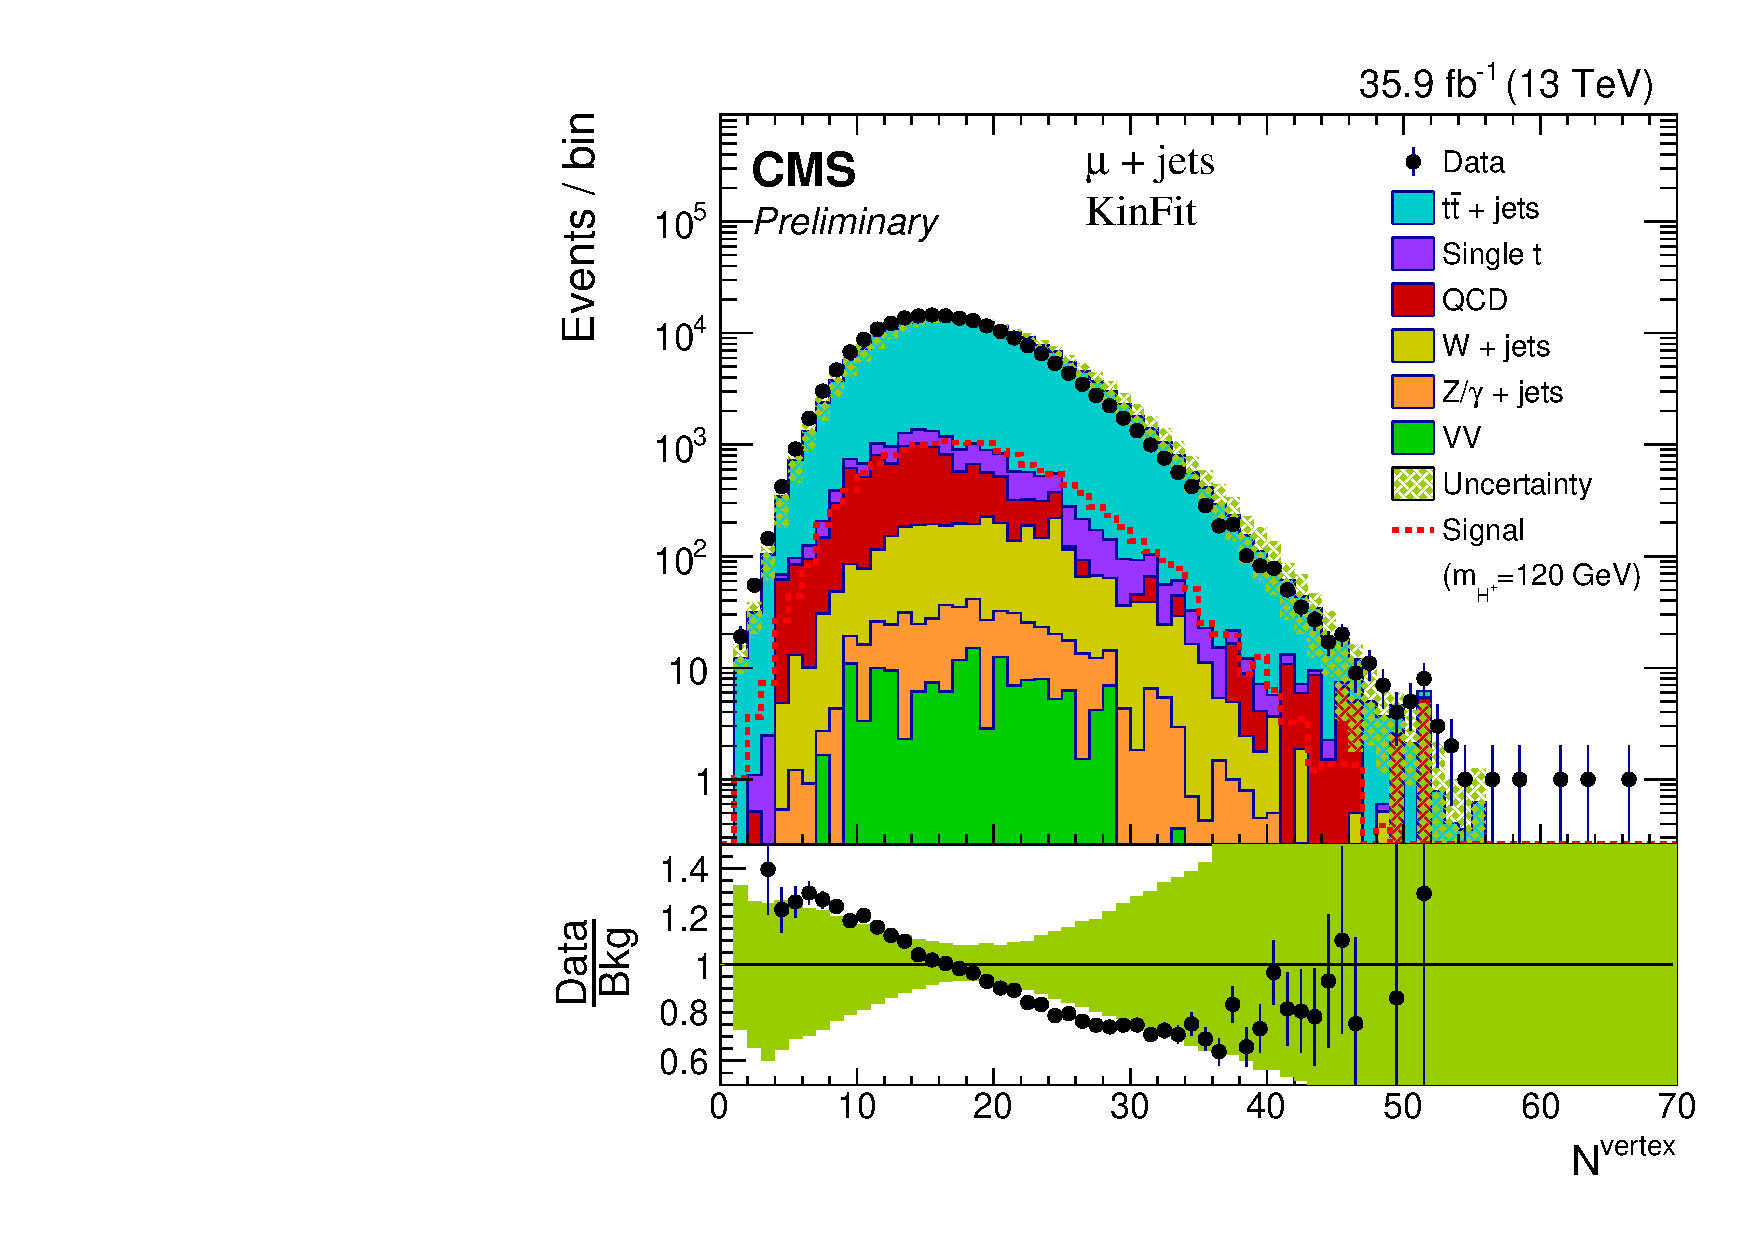
\includegraphics[width=0.49\linewidth]{Image/Muon/KinFit/nvtx_muKinFit.pdf}}
    \subfigure[nvtx distribution \label{subfig:nvtx_eleKinFit} ]
    {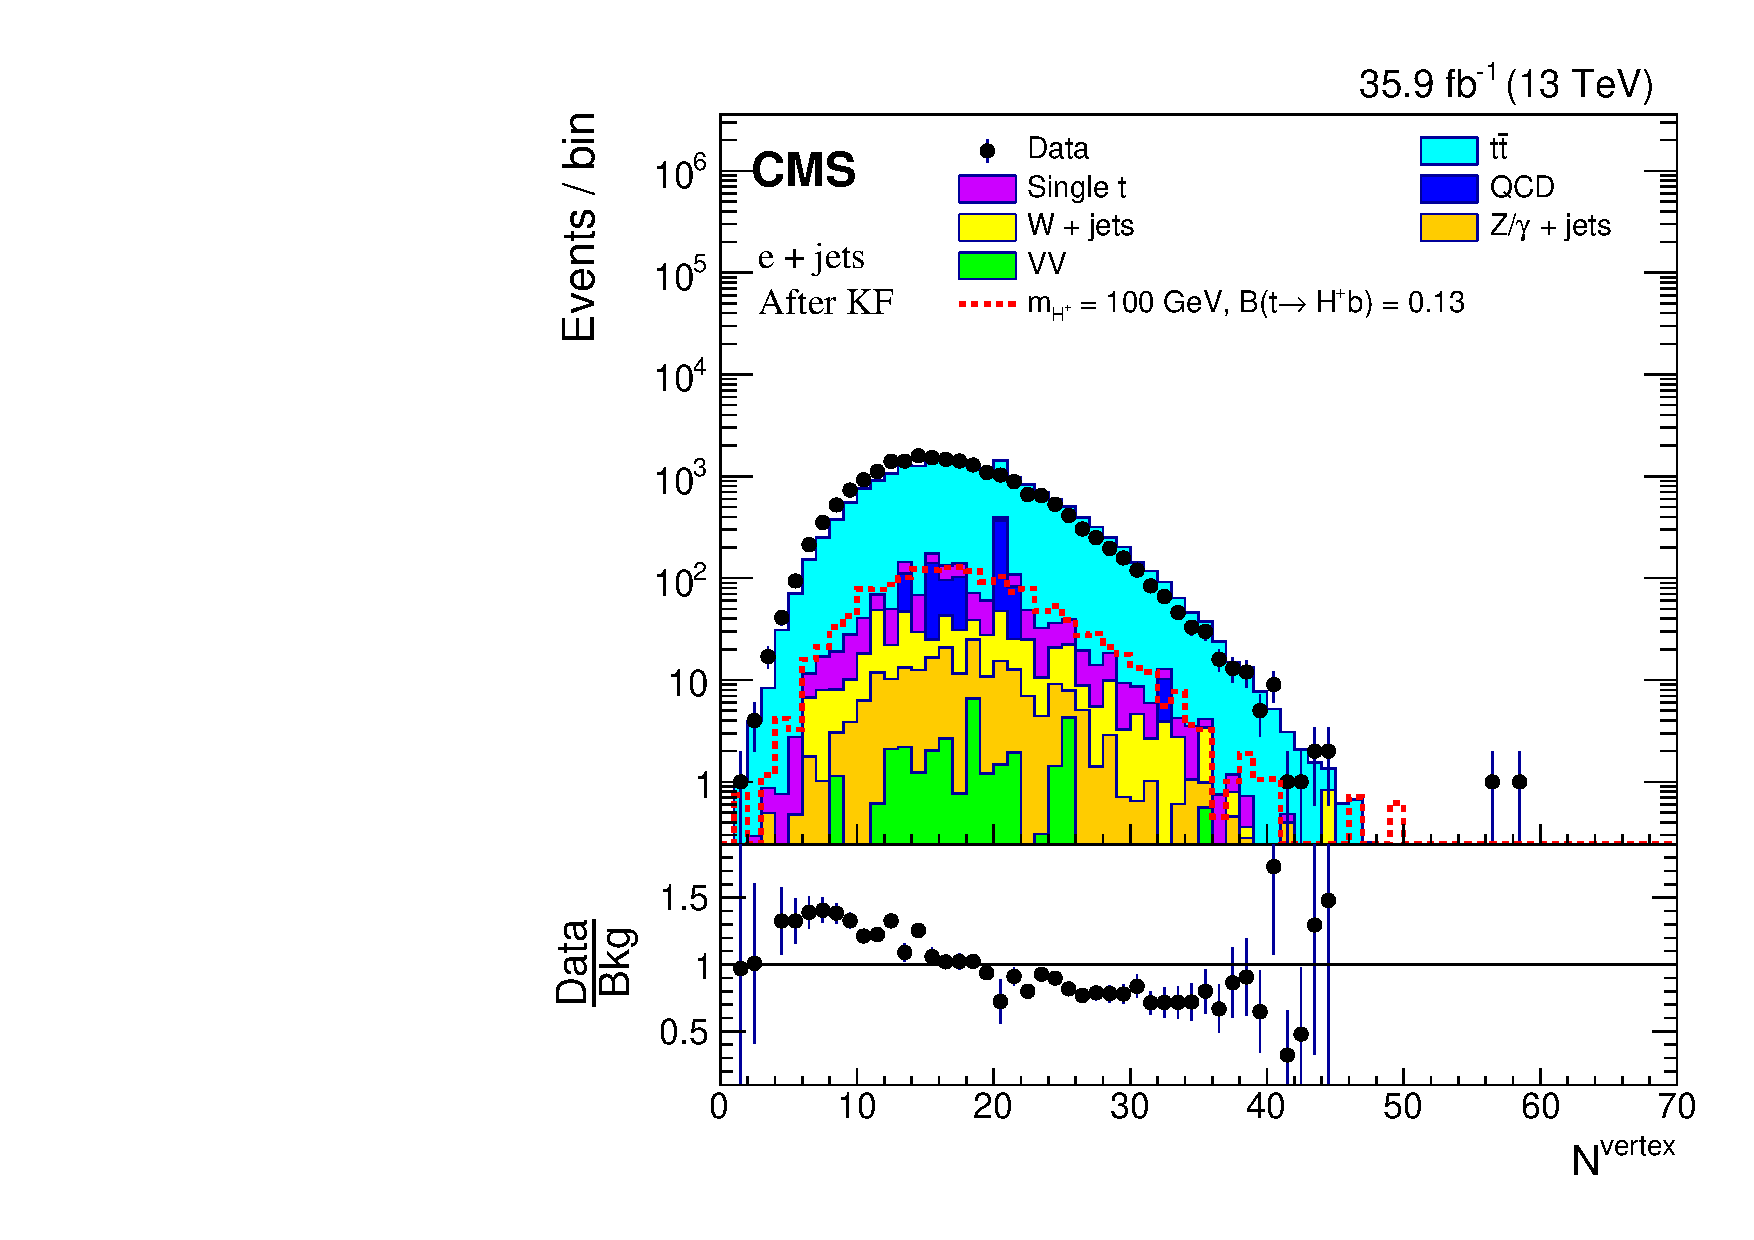
\includegraphics[width=0.49\linewidth]{Image/Electron/KinFit/nvtx_eleKinFit.pdf}}
    \vfil
    \subfigure[$\rho$ distribution \label{subfig:rhoAll_muKinFit}]
    {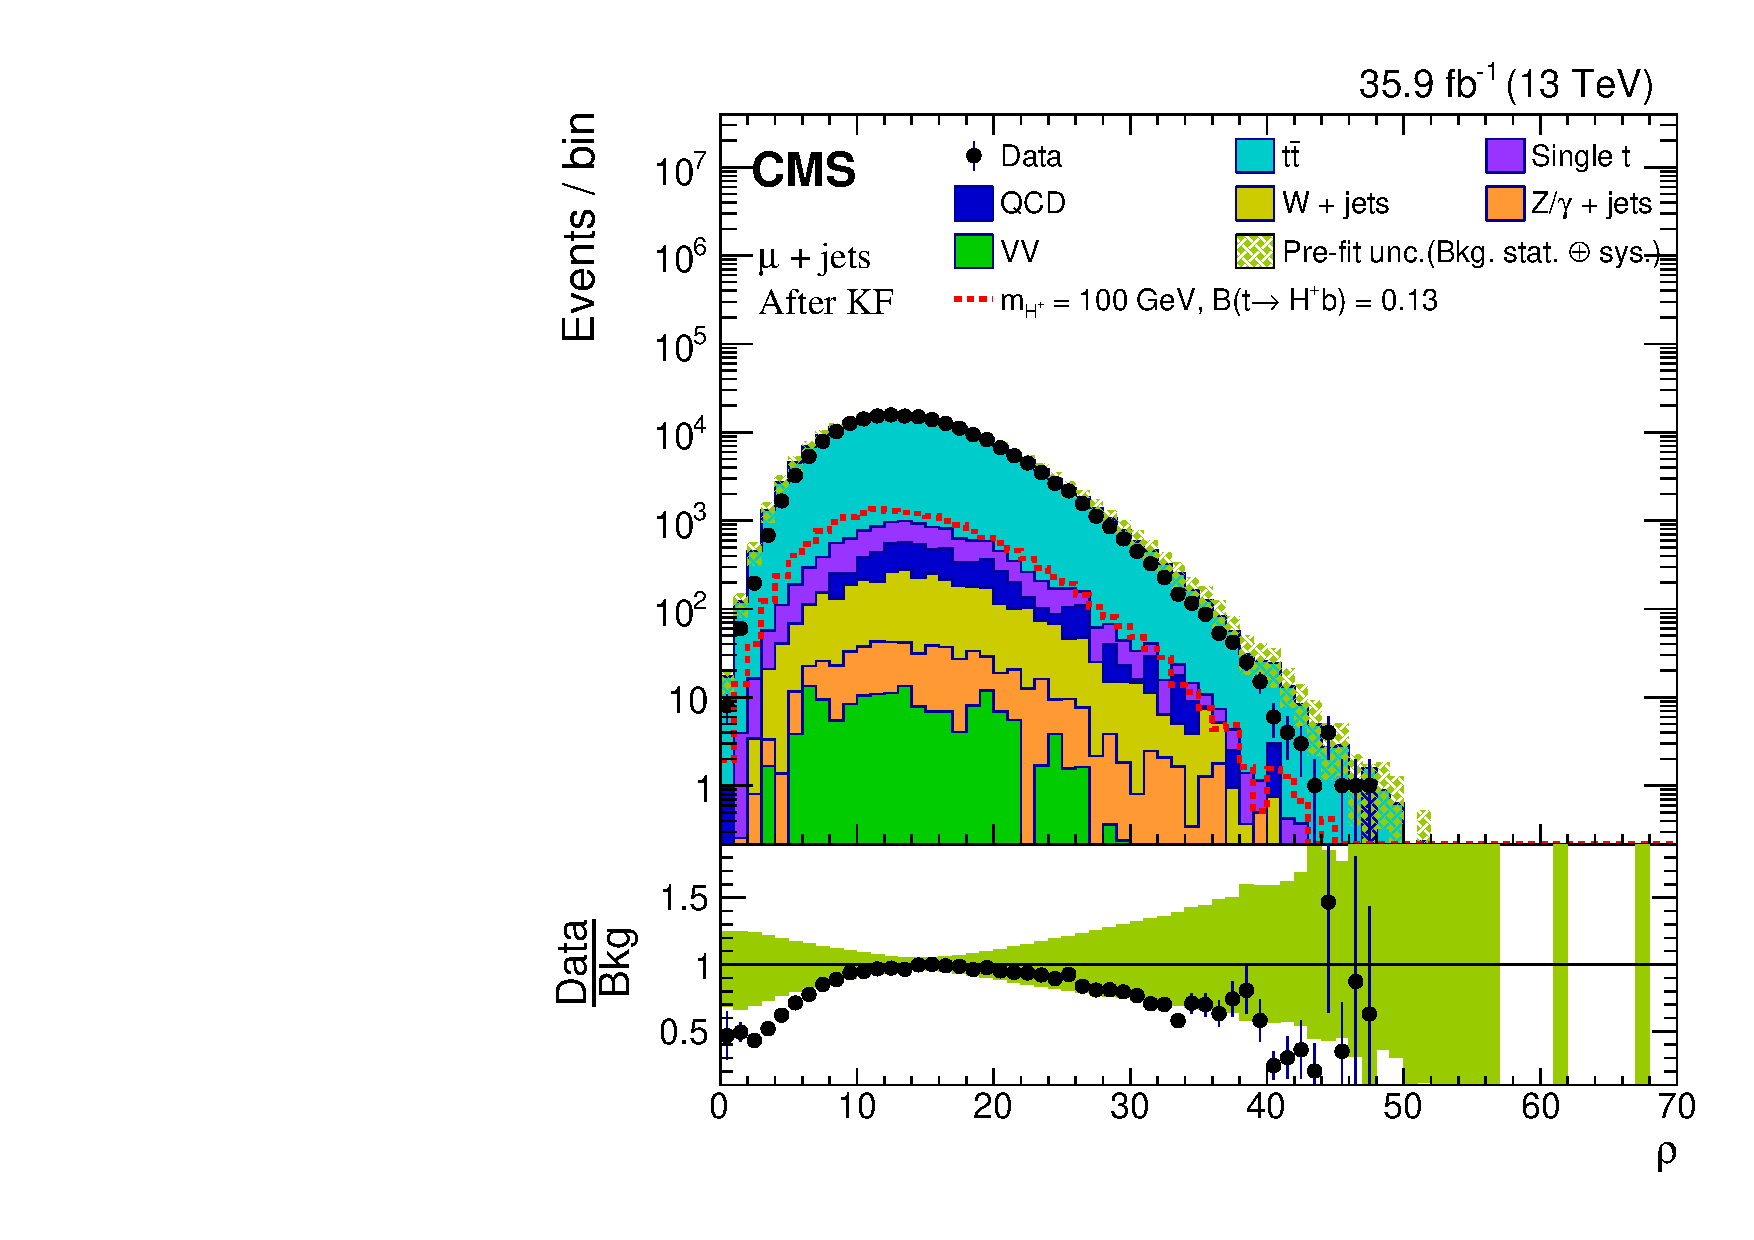
\includegraphics[width=0.49\linewidth]{Image/Muon/KinFit/rhoAll_muKinFit.pdf}}
    \subfigure[$\rho$ distribution \label{subfig:rhoAll_eleKinFit}]
    {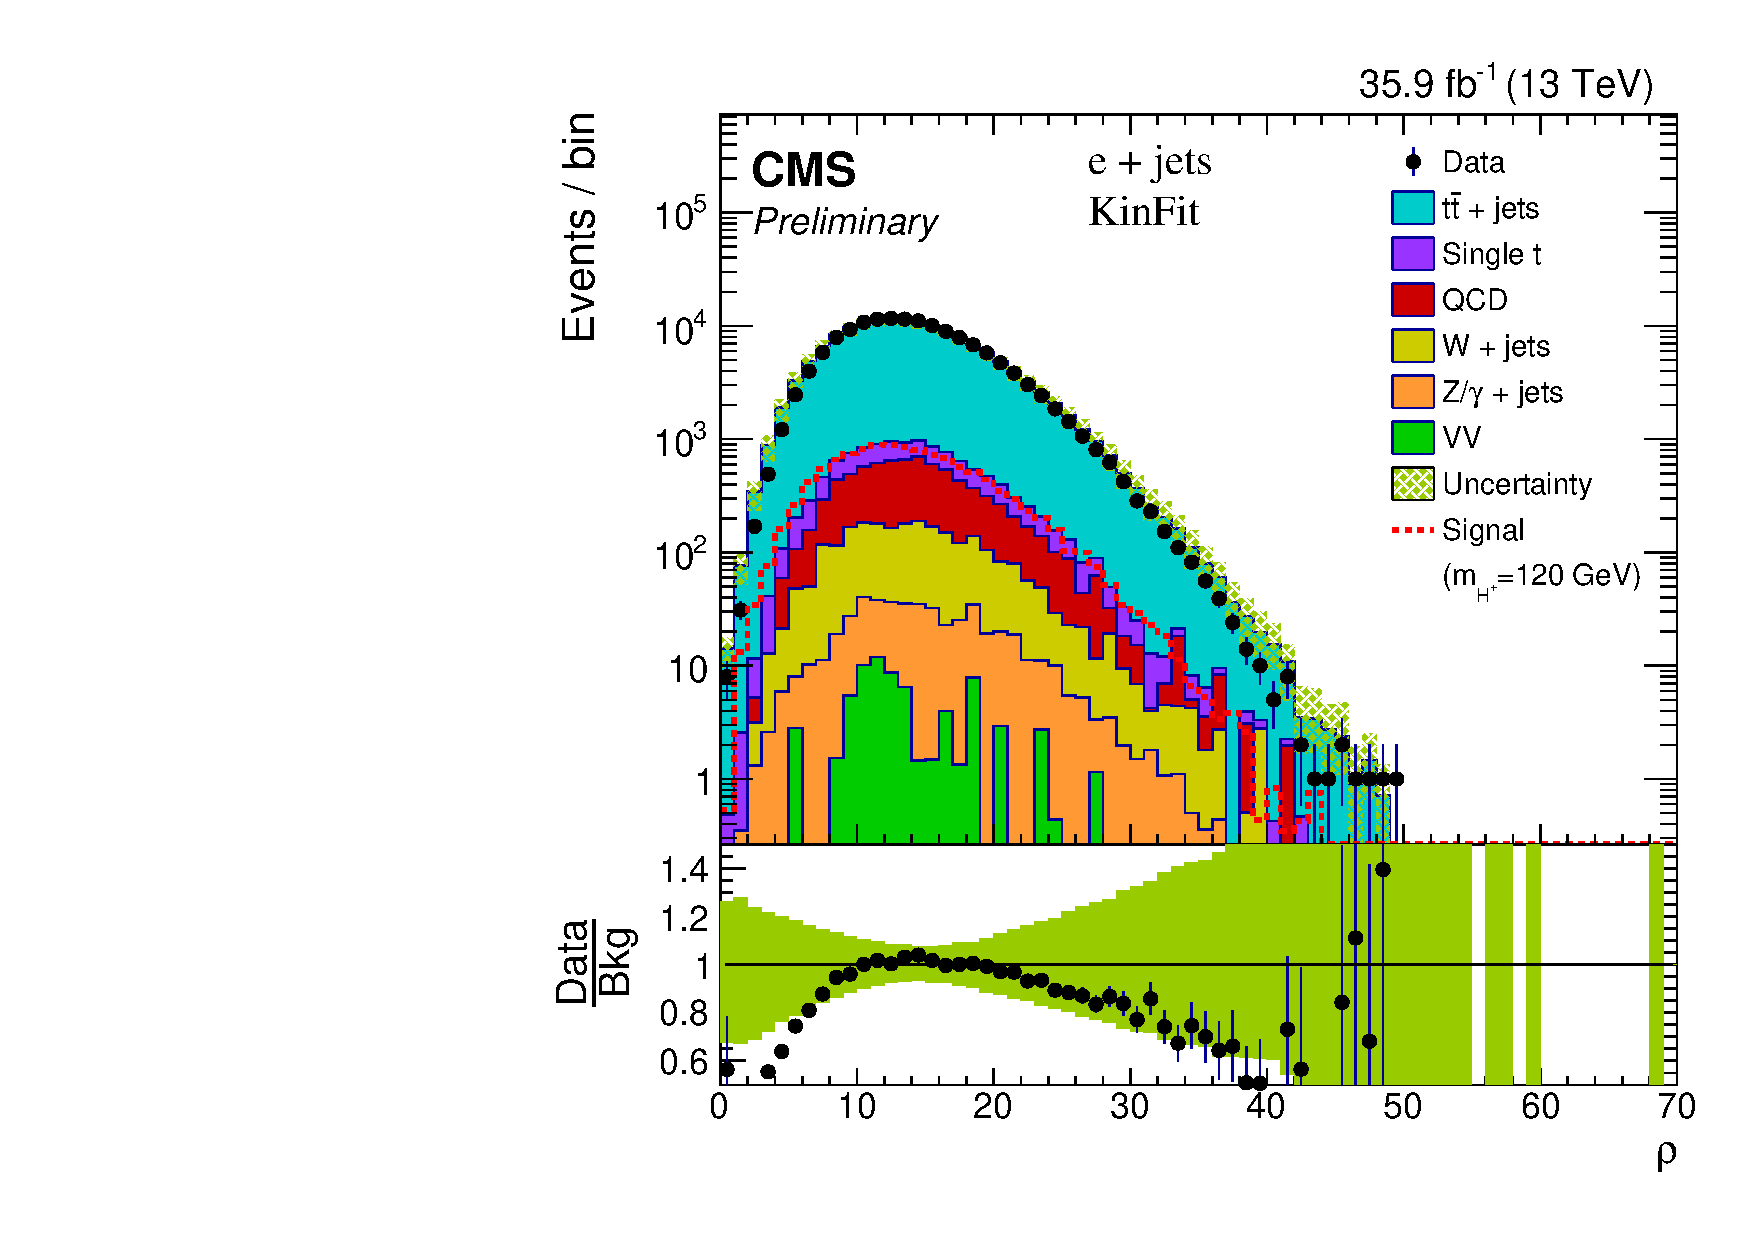
\includegraphics[width=0.49\linewidth]{Image/Electron/KinFit/rhoAll_eleKinFit.pdf}}
    \caption{Number of primary vertices (nvtx) and diffuse offset energy density ($\rho$) distributions 
        for \mujets and \ejets channels. The data-MC agreement is better for $\rho$ compared 
    to the nvtx distribution. For lower values of $\rho$, there is a significant mismatch between data 
    and MC. Similar trend is seen in other analysis 
    as well~\cite{CMS-AN-17-003, CMS-AN-17-116}.}
    \label{fig:nvtxRho}
\end{figure}

%--------------------------------------
% Muon Reconstruction
%--------------------------------------
\subsection{Muon}
\subsubsection{Reconstruction}
Muons are often referred to as minimum ionising particles. Their energy loss is much smaller than 
electrons due to its larger mass. Muon in CMS detector with sufficiently higher \pt can traverse through most of the sub-detectors such as tracker calorimeter and the muon 
detector. Most of the high \pt muons go out of the CMS detector. Due to the presence of a magnetic field, 
trajectories of muon are bent in the CMS detector. The number of hits in the tracker, energy deposit
in the calorimeter and the hits in the muon chambers (DT, CSC, and RPC) are used in the Kalman filtering technique~\cite{FRUHWIRTH1987444}
to reconstruct muon candidates. There are several categories of muons~\cite{Chatrchyan:2012xi} described below:
\begin{itemize}
   \item {\bf{ Standalone Muons}}: These are reconstructed from the muon chambers only. Here, the
       Kalman filtering technique uses the hits from DT, CSC, and RPC to reconstruct standalone muons.
   \item {\bf{ Global Muons}}: The trajectory of a standalone muon is extrapolated up to the tracker. 
       The best pair consisting of the standalone muon and tracker track is selected using the
       Kalman filtering technique. Finally, these two tracks are combined to reconstruct the Global Muon.
       As the global muons are reconstructed starting from the outer part of the CMS detector
       (muon chambers) back to the inner part (strip tracker), this approach of reconstruction is called 
       {\em outside-in}.
   \item {\bf{ Tracker Muons}}: There is an {\em inside-out} approach to reconstruct muons, which 
       starts from the tracks reconstructed in the strip tracker to the energy deposits in the calorimeters
       up to the hits in the muon chamber. Muons reconstructed with this approach are called Tracker muons.
   \item {\bf{ RPC Muons}}: These muons are also reconstructed using the {\em inside-out} approach 
       where only RPC hits of the muon chamber are used~\cite{Goh:2014tra}. 
   \item {\bf{ Calo Muons}}: Some of the reconstructed muon tracks consist of energy deposits
       from the calorimeters. Such muons are called Calo muons.
\end{itemize}

\subsubsection{Identification and Selection}
In the event topology of our interest, there only one lepton (electron or muon) as shown in Figure~\ref{fig:feyn_diag_sig}. These are the 'prompt' lepton coming
directly from the electroweak decay of W bosons.However, there could 'extra'
leptons that come from other sources such as misidentification of light flavored
jets or charged pion decay in case of muons. Medium identification criteria as
recommended by the muon POG are applied to select prompt muons. These are listed
in Table~\ref{tab:muonSel}. The efficiency of medium muon ID as a function of
\pt and $\eta$ is shown in Figure~\ref{fig:muonIsoIDEff} for data and MC.
From this figure, it can be seen that the efficiency at lower \pt is relatively
low compared to that from high \pt. However there is a sudden drop in the
efficiency for data from era BCDEF in the \pt$ > 120$ GeV region. These 
efficiency plots are provided by the muon POG~\cite{muSF}. 
\begin{table}
  \caption{Selection and veto cuts applied on muon.}
 \begin{center}
 \begin{tabular}{ccc}\hline\hline
 Variable & Selection & Veto\\ \hline\hline
 \pt (GeV) & $> 26 $ & $> 15$\\
 $|\eta|$ & $< 2.4$ & $< 2.4$ \\
 Global or tracker muon & Yes & Global \\
 Normalised $\chi^2$ & $< 3$ & \\
 $\chi^2$ local position & $< 12$ & \\
 Tracker kink & $< 20$ &\\
 Segment compatibility & $ > 0.303 $ & \\
 $|d_\mathrm{xy}(\mathrm{vertex})|$ (cm) & $< 0.05$ & \\
 $|d_\mathrm{z}(\mathrm{vertex})|$ (cm) & $< 0.2$ & \\
 Inner track valid fraction & $> 0.8$ & \\
 $I_{\rm rel}^\mu~$ & $< 0.15$ & $< 0.25$\\\hline
 \end{tabular}
 \end{center}
 \label{tab:muonSel}
 \end{table}
\begin{figure}
    \centering
    \subfigure[\label{subfig:muonIDEffPt}]
    {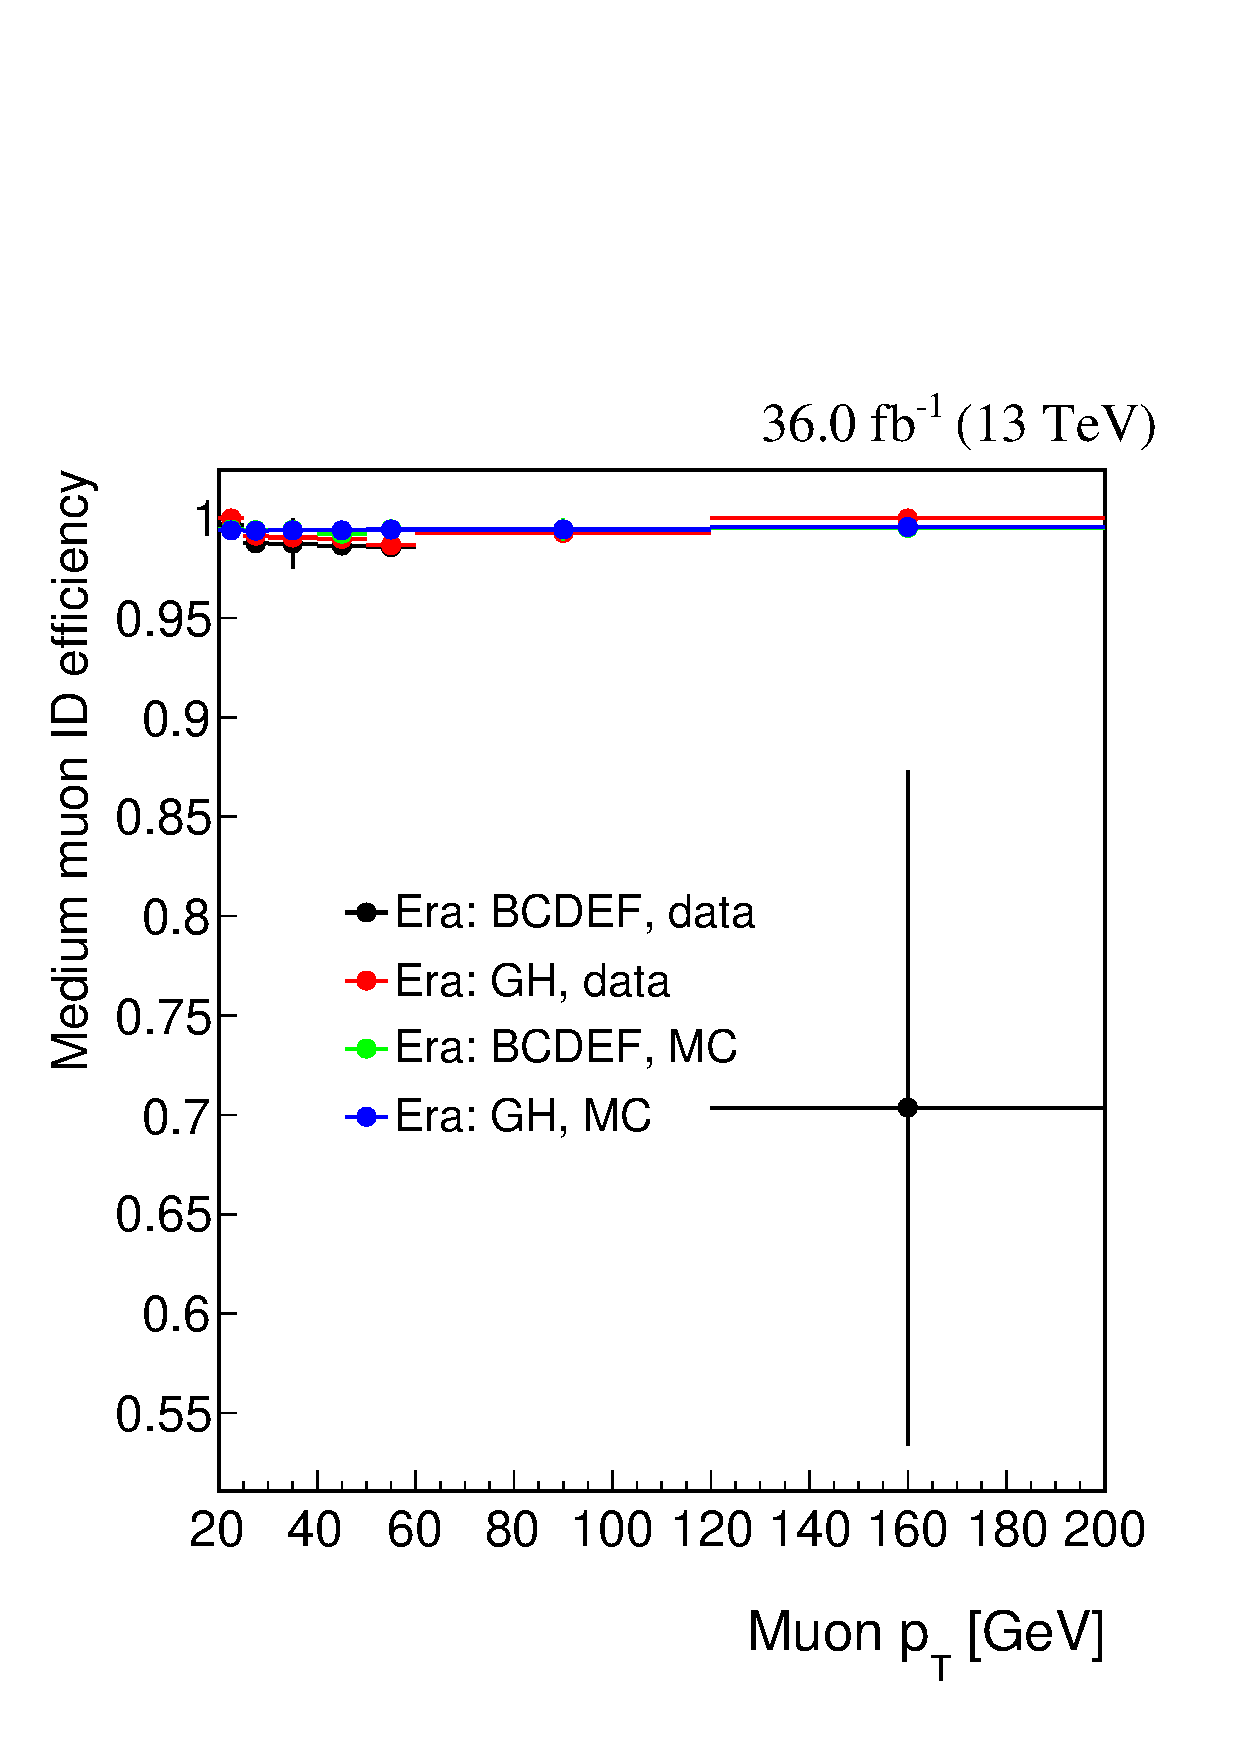
\includegraphics[width=0.49\linewidth]{Image/EffAndSF/muonIDEffPt.pdf}}
    \subfigure[\label{subfig:muonIDEffEta}]
    {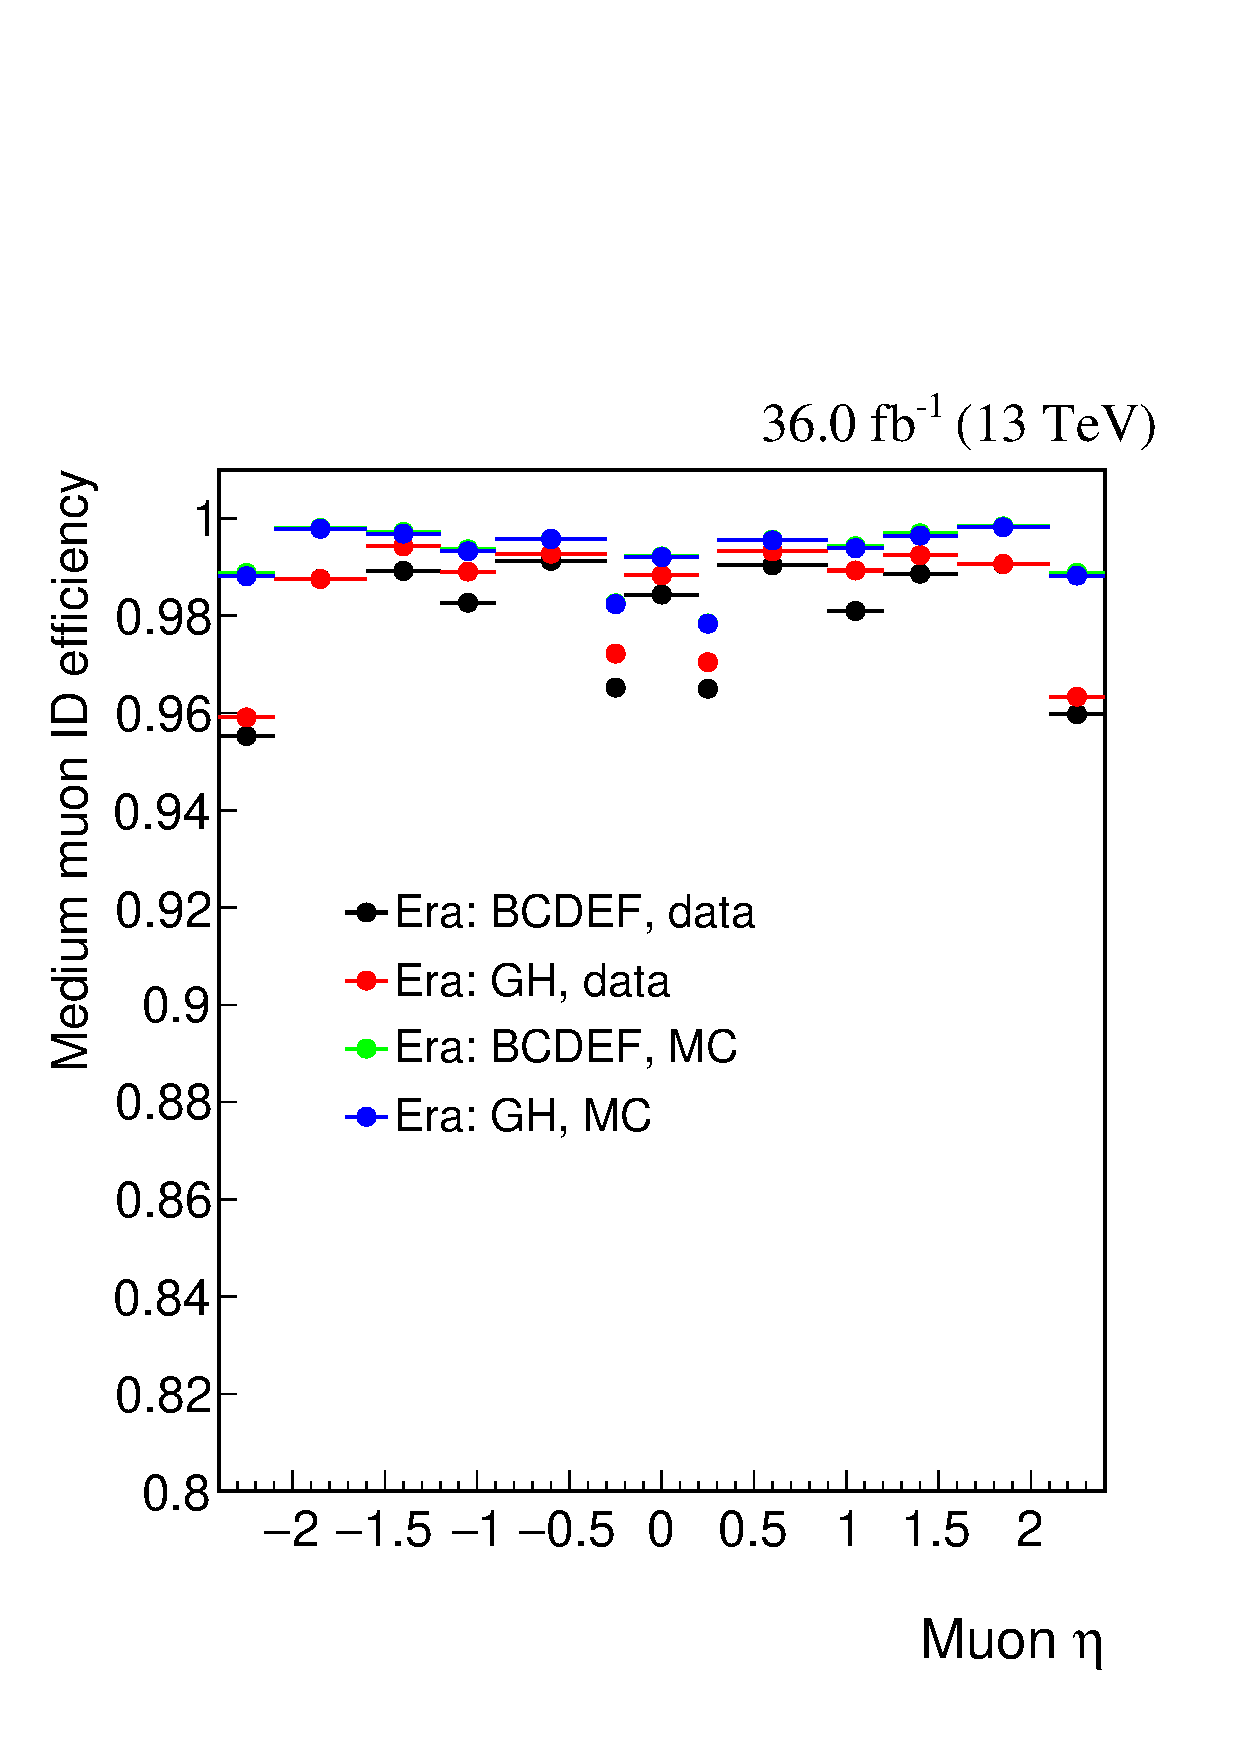
\includegraphics[width=0.49\linewidth]{Image/EffAndSF/muonIDEffEta.pdf}}
    \vfil
    \subfigure[\label{subfig:muonIsoEffPt}]
    {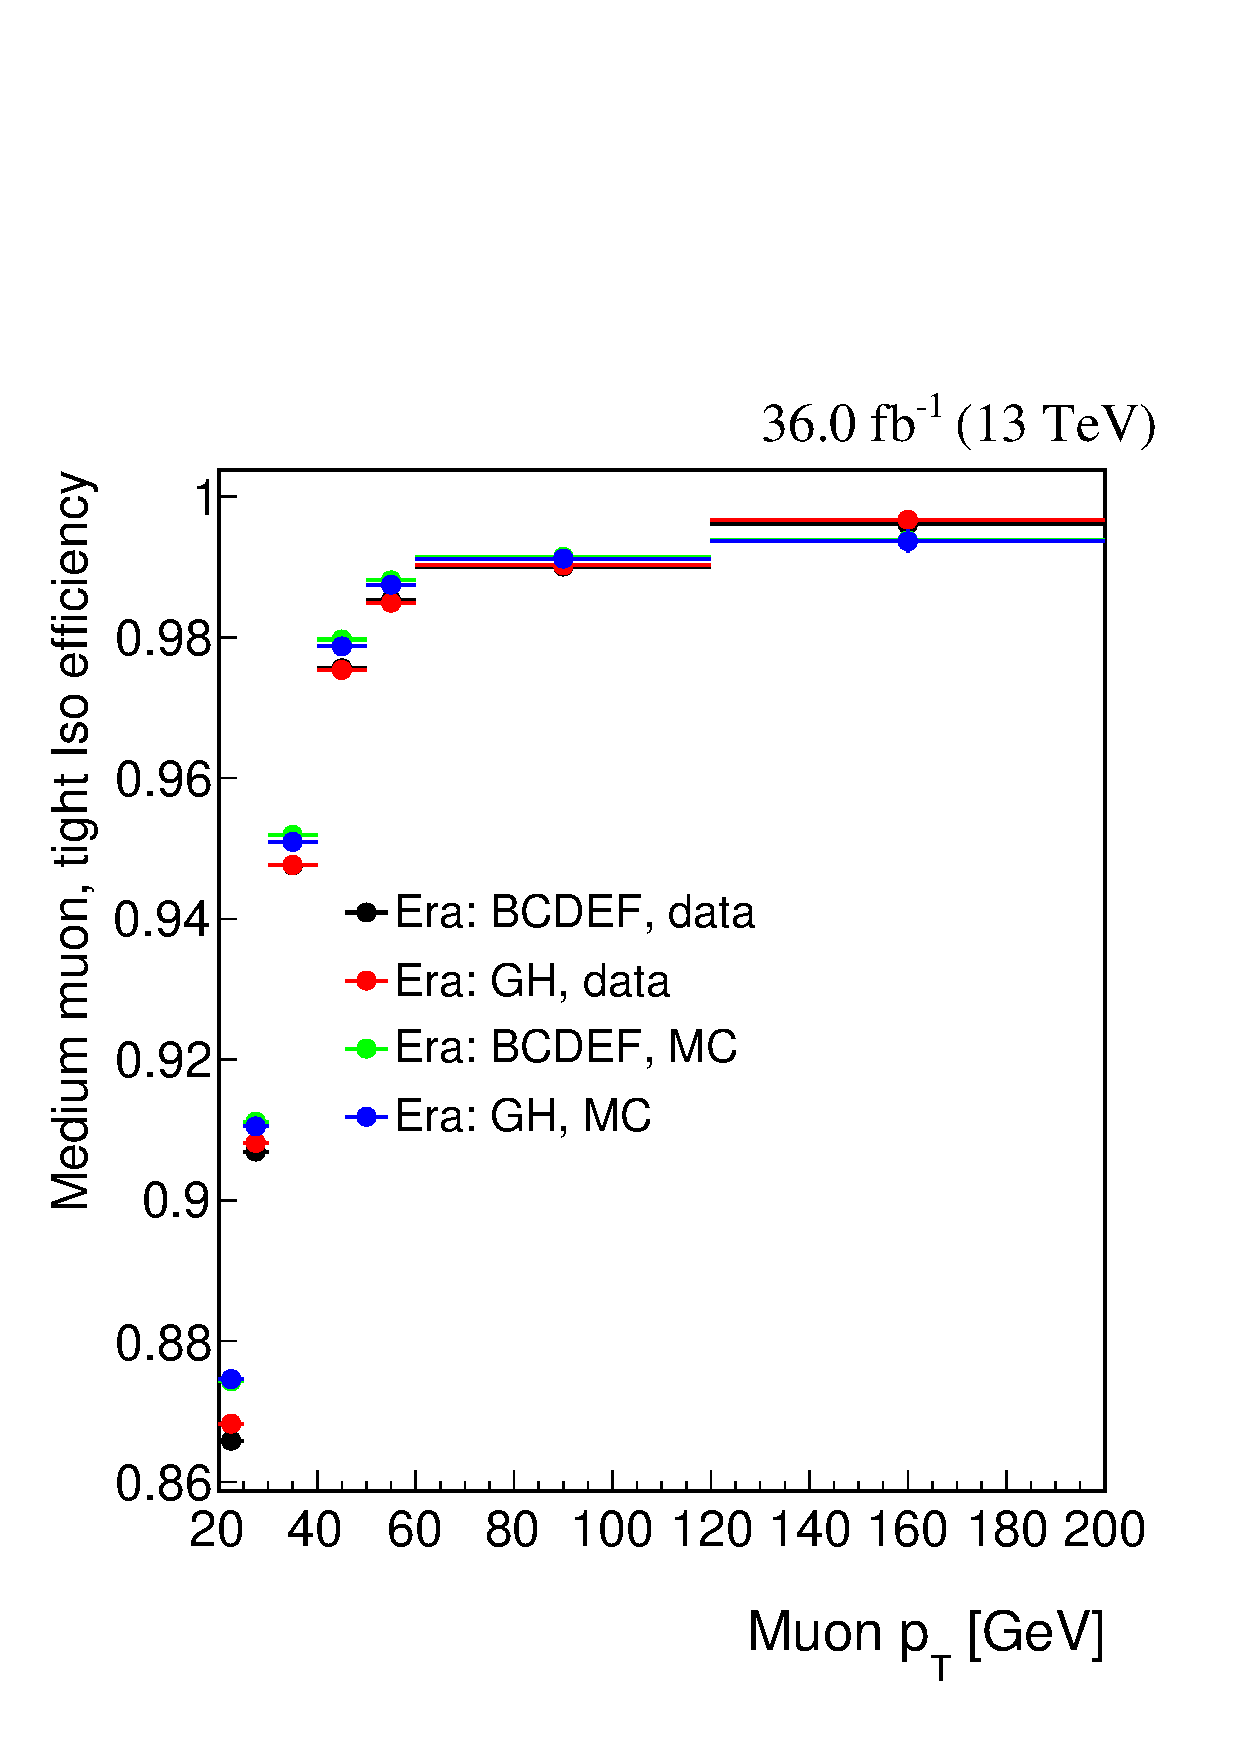
\includegraphics[width=0.49\linewidth]{Image/EffAndSF/muonIsoEffPt.pdf}}
    \subfigure[\label{subfig:muonIsoEffEta}]
    {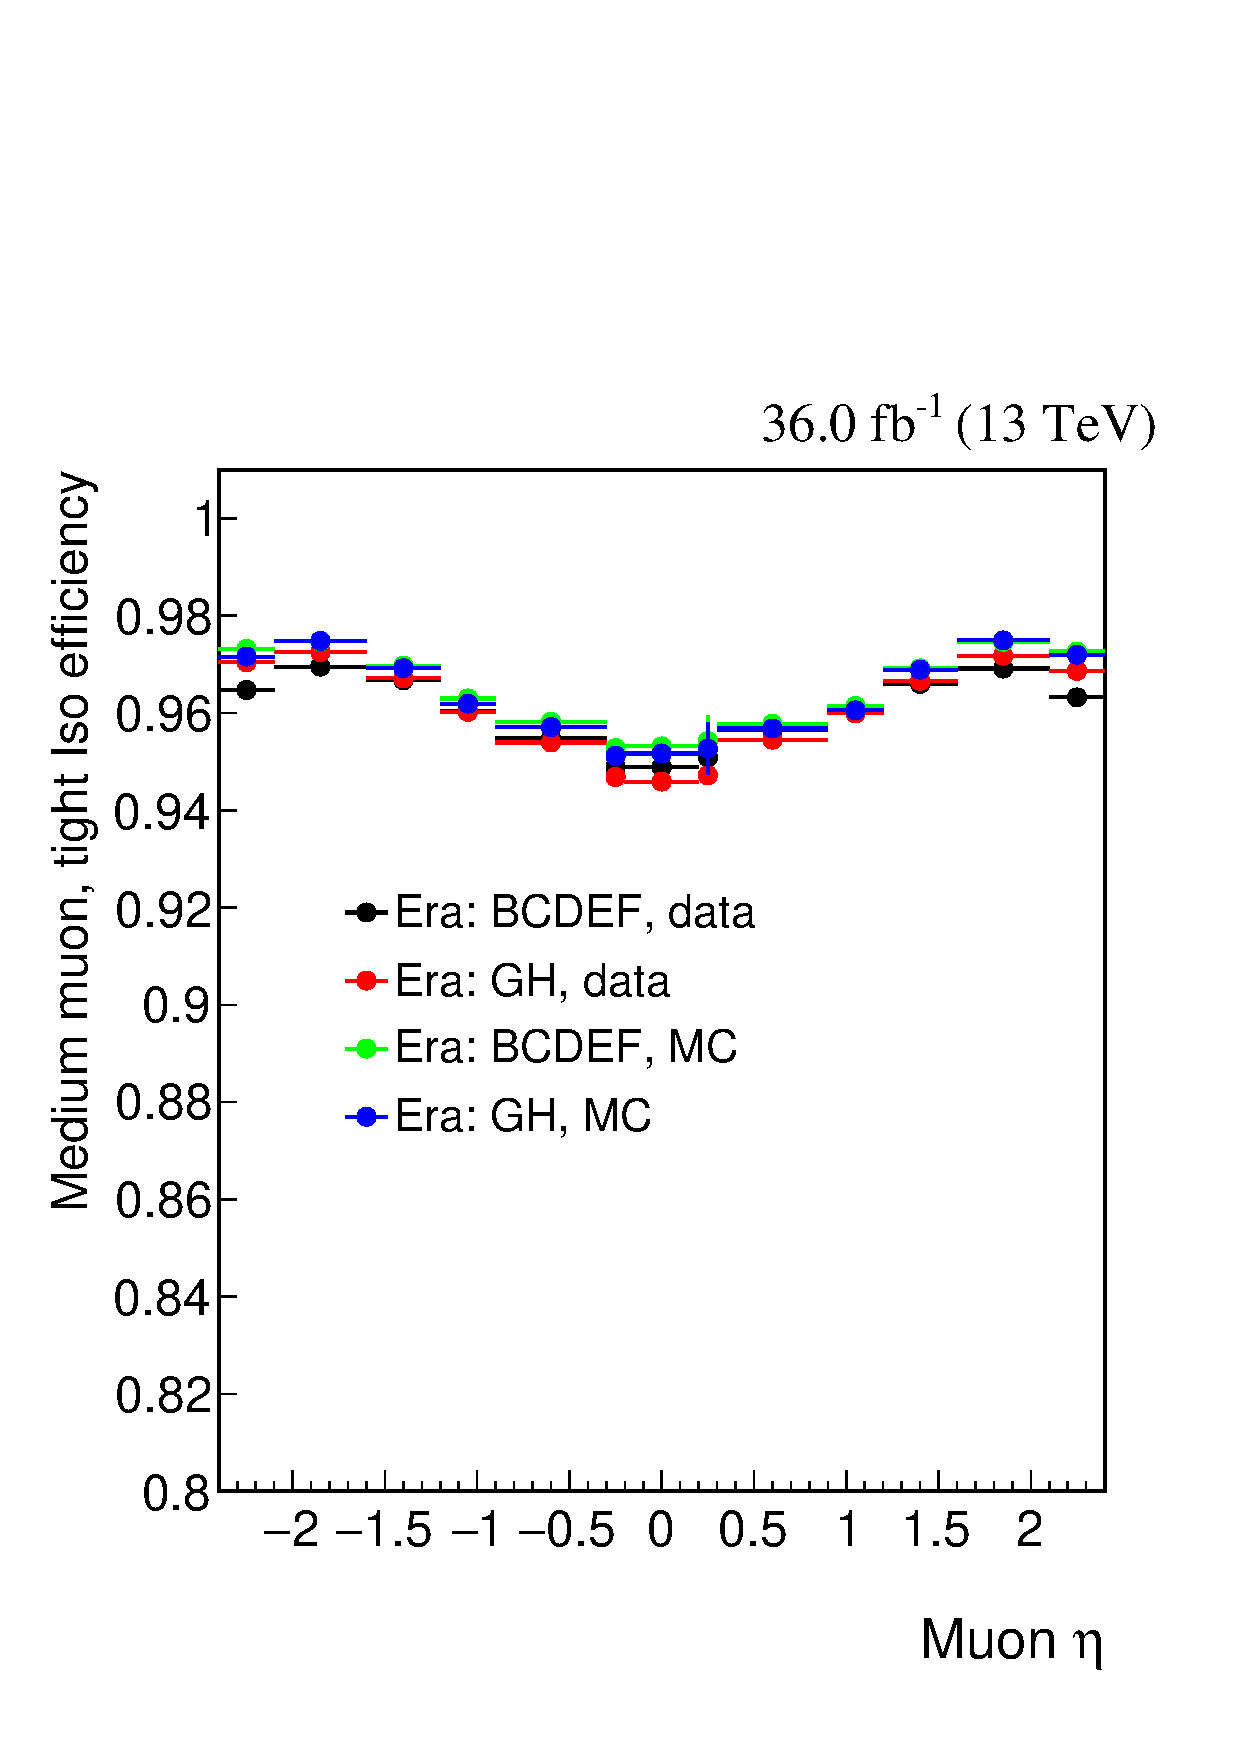
\includegraphics[width=0.49\linewidth]{Image/EffAndSF/muonIsoEffEta.pdf}}
    \caption{ The distribution of efficiencies for medium muon ID and tight relative
    isolation (with medium ID) as a function of \pt and $\eta$ of muon from MC and data
    from different eras.}
    \label{fig:muonIsoIDEff}
\end{figure}

\subsubsection{Rochester correction}
Due to misalignment of the magnetic field and azimuth dependent in-efficiency of 
the muon detector, the efficiency of the muon needs to be corrected. The efficiency
depends on the charge, \pt, $\eta$ and $\phi$ of muon. These corrections referred as 
Rochester correction are applied on data as well as MC samples. The muon \pt is
corrected using Rochester correction tools at 13 TeV~\cite{Bodek:2012id}.
The Rochester scale factors depend on the \pt, $\eta$, $\phi$ and charge of the 
muon. Selection criteria (Table~\ref{tab:muonSel}) on muon are applied after 
Rochester correction.

\subsubsection{Isolation}
A muon track in the pp collision is not necessarily isolated i.e., it can be 
surrounded by other particles. On the other hand, muons from the W decay are 
expected to be isolated. To achieve this, we apply a criterion on the relative
isolation, defined as the \pt sum of all particles excluding the muon within a 
cone of radius 0.4 around the muon direction divided by the muon \pt i.e.
$I_{\rm rel}^\mu=\sum_{i\neq\mu}\pt^i/\pt^\mu$. We use a more specific definition given by  
\begin{equation}
\label{eq:mu_iso}
I_{\rm rel}^\mu=\frac{\sum\pt^{\rm ch}+{\rm max}[(\sum E_T^\gamma+\sum E_T^{\rm neut}-0.5\times\sum\pt^{\rm chPU}),0]}{\pt^\mu},
\end{equation}
where \pt$^{\rm ch}$ is the transverse momentum of charged hadrons; $E_T^\gamma$ and
$E_{T}^{\rm neut}$ are the transverse energy of photons and neutral hadrons; and
\pt$^{\rm chPU}$ is the transverse momentum of charged hadrons associated with the
pileup vertices. The factor $0.5$ takes into account the neutral tracks from the
leading vertex and charged tracks from the pileup vertices~\cite{Sirunyan:2018fpa}.
A tight muon isolation cut of $I_{\rm rel}^\mu < 0.15$ is applied. The efficiency
as a function of \pt and $\eta$ of tight muon isolation with medium ID is shown in
Figure~\ref{fig:muonIsoIDEff} \cite{muSF}.

%--------------------------------------
% Electron Reconstruction
%--------------------------------------
\subsection{Electron }
\subsubsection{Reconstruction}
Electrons are reconstructed using the PF algorithm~\cite{CMS-PAS-PFT-09-001, CMS-PAS-PFT-10-001} 
based on the tracks in the tracker and energy deposits in the electromagnetic calorimeter
~\cite{Khachatryan:2015hwa}. Being a charged particle electrons radiate as they travel inside the huge
magnetic field of the CMS. Thus the energy deposited by an electron in the ECAL is
spread in $\eta$ and $\phi$ direction across several crystals. The energy deposited
in various crystals are clustered using "hybrid" algorithm in the barrel and "multi-5x5"
in endcap part of the ECAL. For given hits in the innermost layer of the tracker, the 
Kalman Filter technique is used to find hits in the next layer of the tracker. The hits collected
from all layers of the tracker is mapped to the energy deposit in the ECAL to form 
an electron candidate. To take care of the effect of bremsstrahlung, the "Gaussian sum 
filter" method is used to fit the tracks. The electron charge is estimated from the 
curvature of the electron track and by matching associated KF track with GSF tracks. The vector joining (SC, beam-spot) and (SC, first hit of the GSF track) in $\phi$ is also used for
electron charge estimation. The measurements from tracker and ECAL are combined to estimate
the electron momentum~\cite{Khachatryan:2015hwa}.

\subsubsection{Identification and Selection}
To select prompt electrons, medium cut-based ID as listed in Table~\ref{tab:eleSel} is
used. Electrons with \pt$ > 30$\,GeV and $|\eta| <$ 2.5 are excluded. 
\begin{table}
  \caption{Selection and veto cuts applied on electron.}
 \label{tab:eleSel}
 \centering
\begin{adjustbox}{max width=\textwidth}
 \begin{tabular}{ccccc}\hline\hline
 Variable & \multicolumn{2}{c}{Selection} & \multicolumn{2}{c}{Veto}\\
  & $|\eta_{\rm sc}|\leq 1.479$ & $|\eta_{\rm sc}|>1.479$ & $|\eta_{\rm sc}|\leq 1.479$ & $|\eta_{\rm
 sc}|>1.479$\\\hline\hline
 \pt (GeV) & $> 30$ & $> 30$ & $> 15$ & $> 15$\\
 $|\eta|$ & $< 2.5$ & $< 2.5$ & $ -$ & $- $\\
 full $5\times 5$ $\sigma_{i\eta i\eta}$    & $< 0.00998$   & $< 0.0298$    & $< 0.0115 $   & $<0.037$\\
 $|\Delta\eta({\rm sc},{\rm track})|$       & $< 0.00311$   & $< 0.00609$   & $< 0.00749$   & $<0.00895$\\
 $|\Delta\phi({\rm sc},{\rm track})|$       & $< 0.103$     & $< 0.045$     & $< 0.228$     & $< 0.213$\\
 $E_{{\rm had}}/E_{{\rm em}}$               & $< 0.253$     & $< 0.0878$    & $< 0.356$     & $<0.211$\\
 $I_{\rm rel}^e$                            & $< 0.0821$    & $< 0.0695$    & $< 0.175$    & $<0.159$\\
 $|\frac{1}{E}-\frac{1}{p}|$ (GeV)$^{-1}$   & $< 0.134$     & $< 0.13$      & $< 0.299$ &$<0.15$\\
 Missing inner hits                         & $\le 1$       & $\le 1$       & $\le 2$       & $\le 3$\\
 Conversion veto                            & Yes           & Yes           & Yes           & Yes\\
 $|d_{xy}({\rm vertex})|$ (cm)              & $< 0.05$      & $< 0.10$       &$<0.05$      & $<0.05$\\
 $|d_z({\rm vertex})|$ (cm)                 & $< 0.10$      & $< 0.20$       & $<0.1$      &$<0.1$\\\hline
 \end{tabular}
\end{adjustbox}
 \end{table}

A brief description of the variables listed in Table~\ref{tab:eleSel} is given below:
\begin{itemize}
    \item full $5\times 5$ $\sigma_{i\eta i\eta}$ is defined as~\cite{Khachatryan:2015hwa} 
    \begin{equation}
    \sigma_{i\eta i\eta}=\sqrt{\sum(0.0175\times\eta_i+\eta^{\rm seed}_{\rm cryst}-\bar{\eta}_{5\times 5})^2\times w_i]/\sum w_i}, \quad w_i = 4.2 + \log(E_i/E_{5\times 5})
    \label{eq:sIeIe}
    \end{equation}
    The summation is carried over the $5\times 5$ matrix around the highest $E_T$ crystal of the supercluster.
    \item $|\Delta\eta({\rm sc},{\rm track})|$: Difference in $\eta$ of the supercluster and the electron track.
    \item $|\Delta\phi({\rm sc},{\rm track})|$: Difference in $\phi$ the supercluster and the electron track.
    \item $E_{\rm had}/E_{\rm em}$: Ratio of the electron energy deposited in the HCAL and ECAL.
    \item $|\frac{1}{E}-\frac{1}{p}|$: $E$ is the energy of the supercluster and $p$ is the track momentum at
    the point of closest approach from the PV.
    \item Missing inner hits: Number of missing hits in the strip tracker.
    \item $|d_{xy}({\rm vertex})|$: Distance of closest approach of the electron track from the PV in the $xy$ plane.
    \item $|d_{z}({\rm vertex})|$: Difference in the $z$-coordinate of the PV and the electron track.
\end{itemize}
The relative isolation $I_{\rm rel}^e$ and conversion veto of Table~\ref{tab:eleSel}
are discussed in Sections~\ref{s:ele_iso} and \ref{s:ele_conv_rej}. The efficiency of medium and 
veto electron ID as a function of \pt and $\eta$ is shown in Figure~\ref{fig:eleIDEff} \cite{eleSF}.
\begin{center}
\begin{figure}
   \subfigure[Efficiency for medium ID]
   {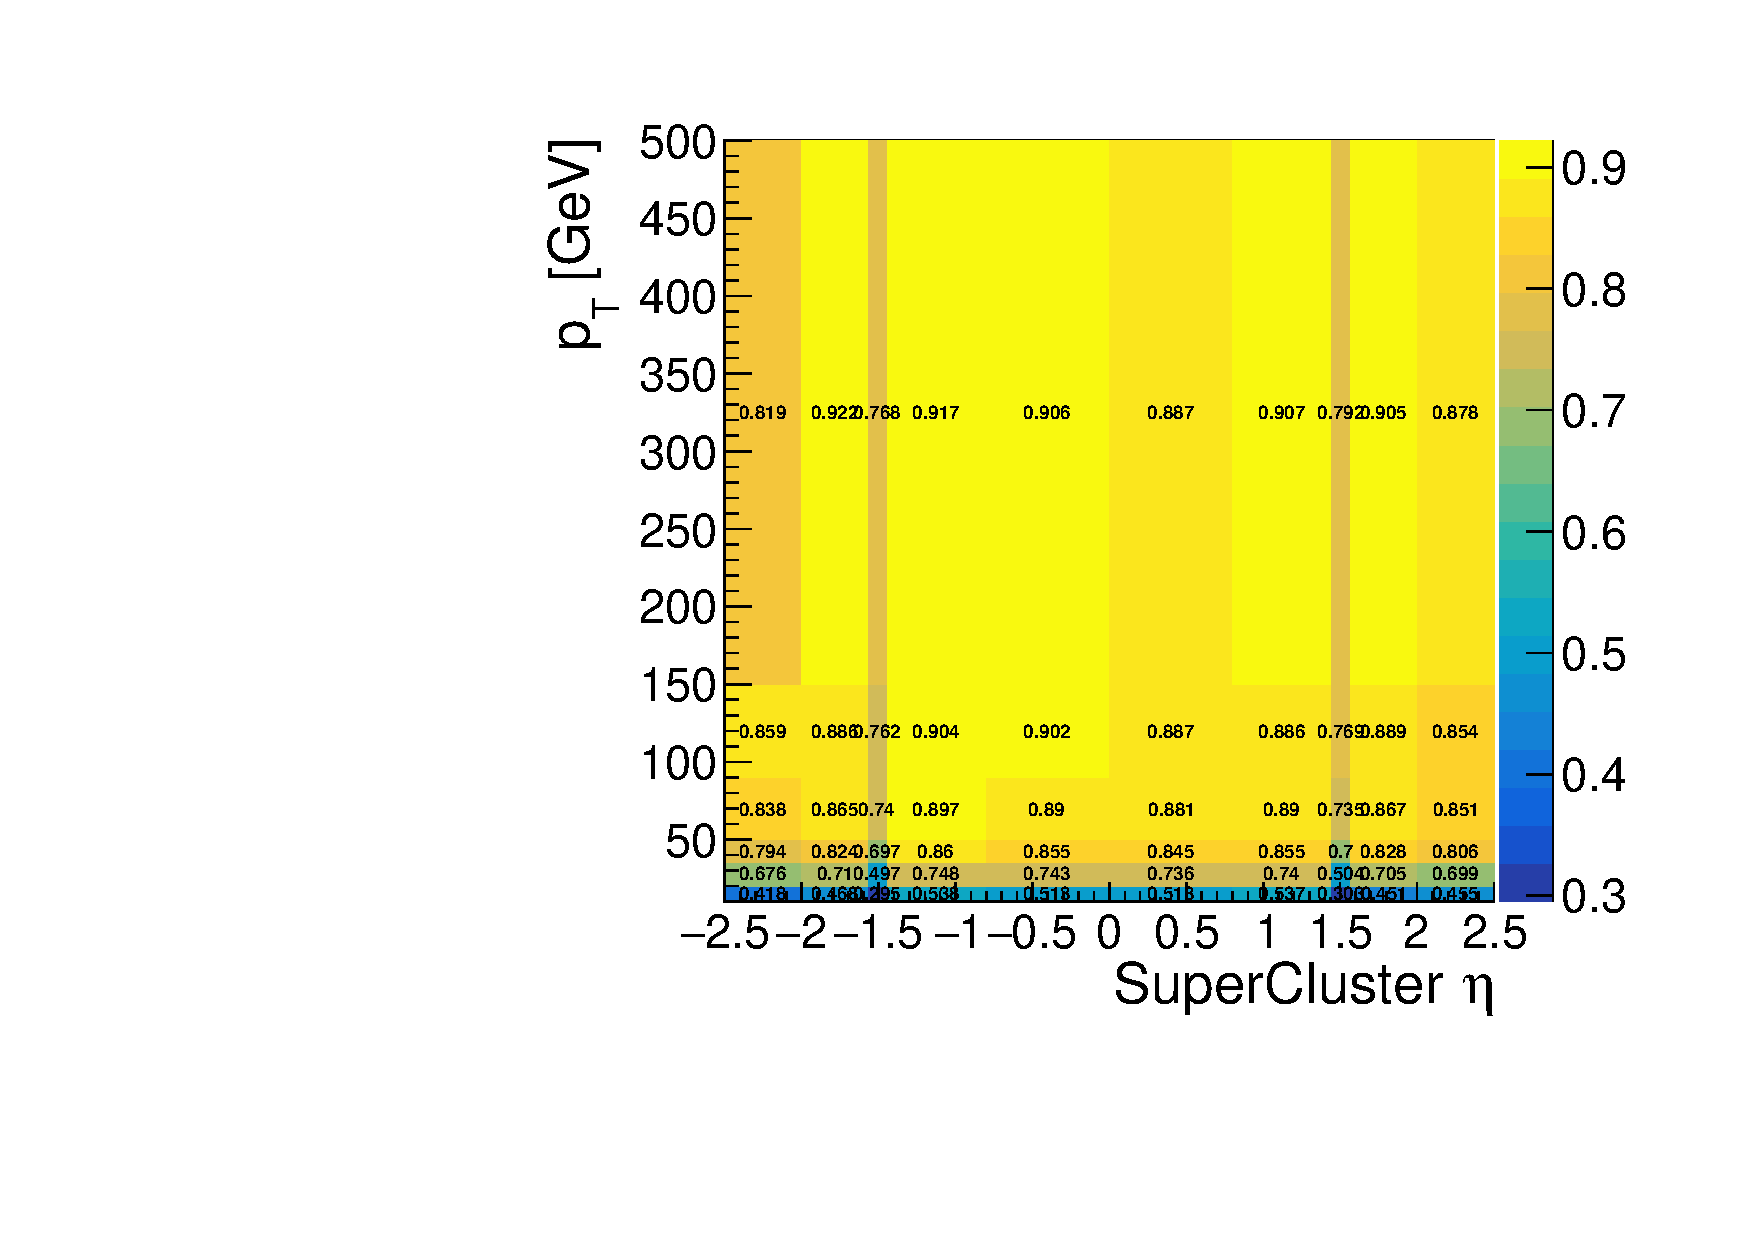
\includegraphics[width=0.49\linewidth]{Image/EffAndSF/eleMediumIDEff_mc2D.pdf}}
   \subfigure[Efficiency for veto ID]
   {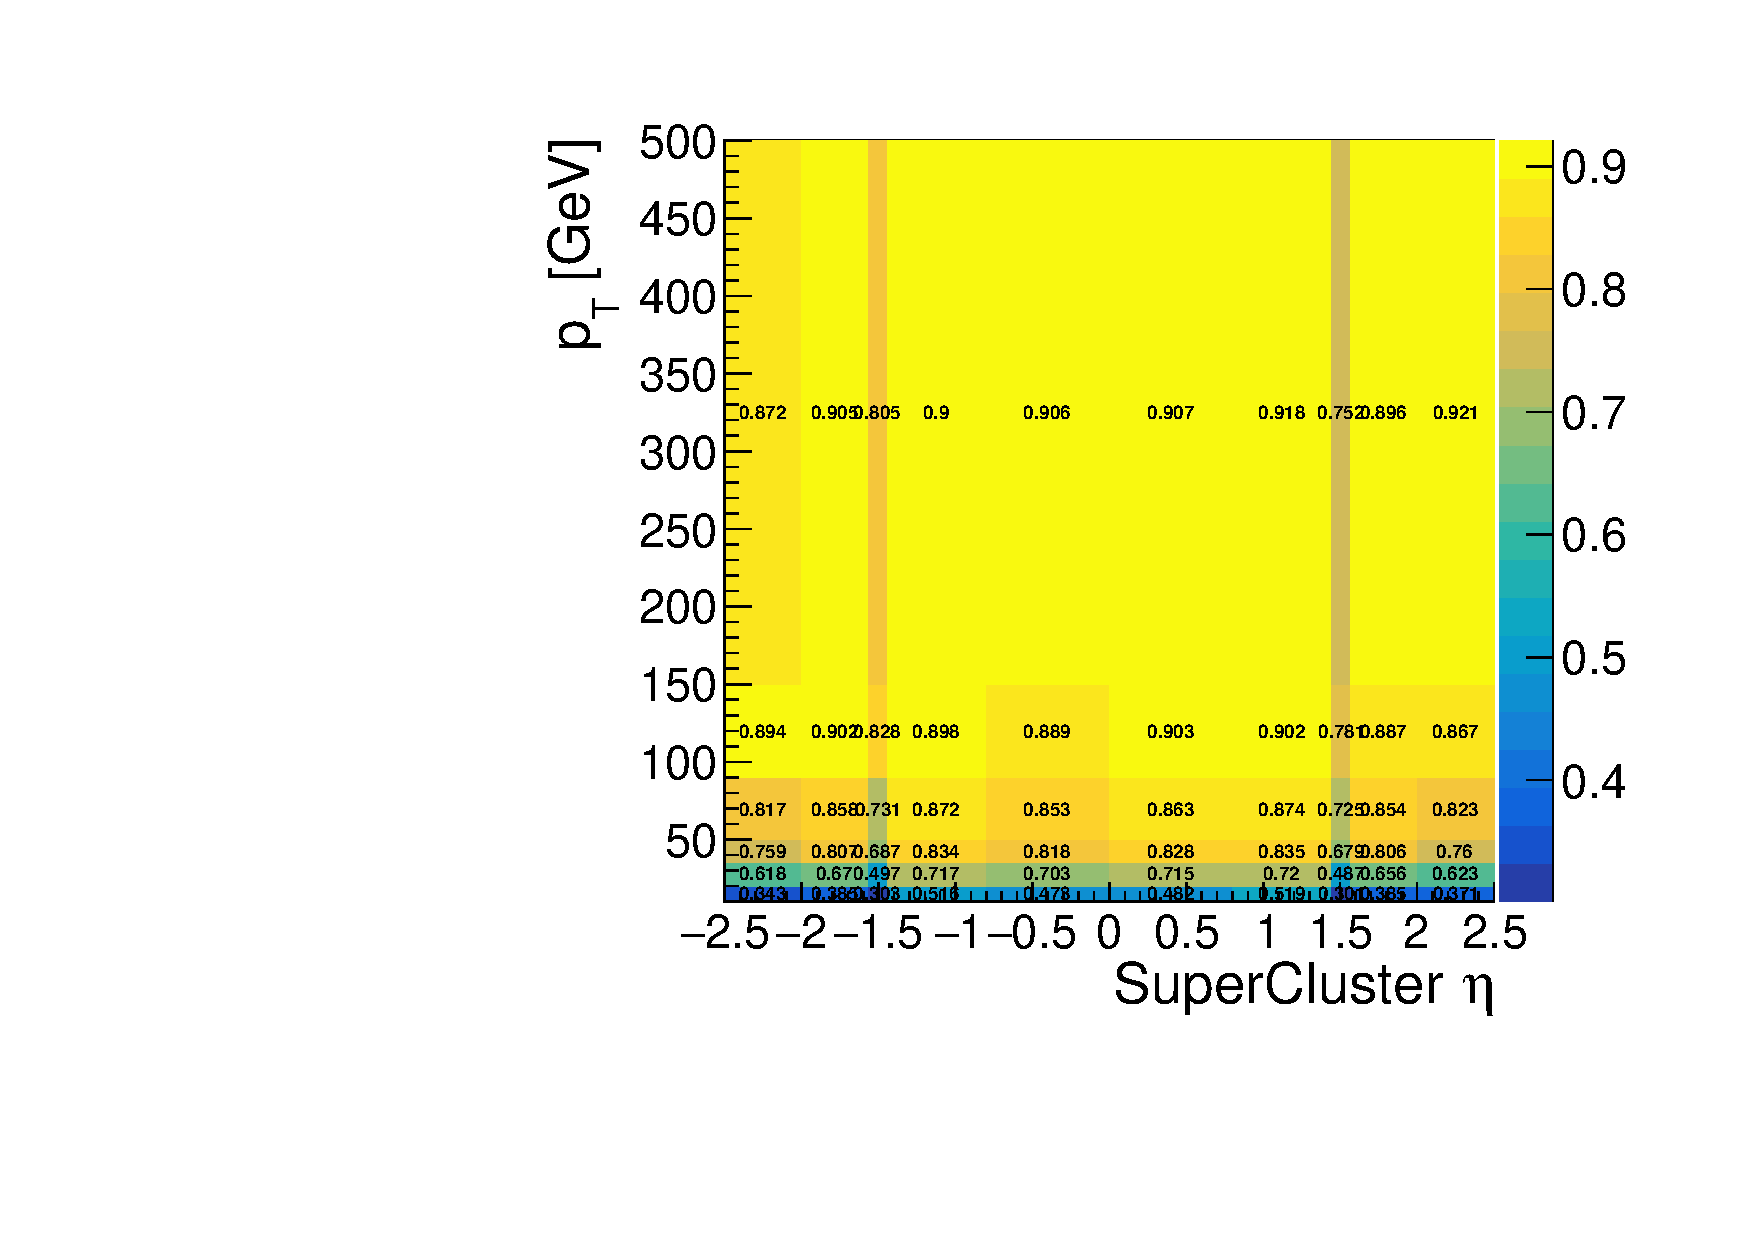
\includegraphics[width=0.49\linewidth]{Image/EffAndSF/eleMediumIDEff_data2D.pdf}}
\caption{ The distribution of efficiency for medium and veto electron ID.} 
\label{fig:eleIDEff}
\end{figure}
\end{center}

\subsubsection{Isolation}
\label{s:ele_iso}
The relative isolation of an electron is given by:
\begin{equation}
\label{eq:ele_iso}
I_{\rm rel}^e= \frac{\sum\pt^{ch}+{\rm max}[(\sum E_T^\gamma+\sum E_T^{\rm neut}-\rho\times A_{\rm eff}),0]}{\pt^e},
\end{equation}
where $\rho$ is as defined in Eq.~(\ref{eq:rho}) and $A_{\rm eff}$ is the effective
area. (To get $\rho$ for $I_{\rm rel}^e$ from {\em MINIAOD}, {\em fixedGridRhoFastjetAll} tag is used.)
These two quantities are used to correct electron isolation from pileup.
The effective area for different $\eta_{\rm sc}$ are shown in Table~\ref{tab:EA}. The
tight isolation cut of $I_{\rm rel}^e < 0.0821 (0.0695)$ is applied on electrons from
the barrel (endcap) regions.
\begin{table}
 \caption{Effective area for different $\eta_{\rm sc}$ range.}
 \begin{center}
 \begin{tabular}{cc}\hline\hline
     Super-cluster pseudorapidity $(\eta_{\rm sc}$) & $A_{\rm eff}$ \\ \hline\hline
     $0.0 \leq \eta_{\rm sc} < 1.0 $ & $0.1703$ \\
     $1.0 \leq \eta_{\rm sc} < 1.5 $ & $0.1715$ \\
     $1.5 \leq \eta_{\rm sc} < 2.0 $ & $0.1213$ \\
     $2.0 \leq \eta_{\rm sc} < 2.2 $ & $0.1230$ \\
     $2.2 \leq \eta_{\rm sc} < 2.3 $ & $0.1635$ \\
     $2.3 \leq \eta_{\rm sc} < 2.4 $ & $0.1703$ \\
     $2.4 \leq \eta_{\rm sc} $ & $0.2393$ \\\hline
 \end{tabular}
 \end{center}
 \label{tab:EA}
 \end{table}

\subsubsection{Conversion rejection}
\label{s:ele_conv_rej}
Some of the reconstructed electrons are end products of photon conversion inside the tracker.
While selecting prompt electrons these secondary electrons need to be rejected.
The tag used for conversion rejection is {\em reducedEgamma:reducedConversions}.
As the secondary electrons don't have hits in the innermost layer of the tracker~\cite{Khachatryan:2015hwa},
one can use this feature to reject them.
By fitting the electron tracks, these secondary electrons are also rejected ~\cite{Khachatryan:2015hwa}.

%--------------------------------------
% Jet Reconstruction
%--------------------------------------
\subsection{Jet}
\label{s:jet_reco}
\subsubsection{Reconstruction}
Due to color confinement~\cite{Polyakov:1976fu}, the quarks and gluons produced in pp collisions cannot exist in the free states.
Instead, they hadronise into a cluster of colorless particles such as hadrons, leptons, and photons.
We form a jet out of these particles, emanating in a cone around the initial direction quarks and gluons.
In CMS the PF algorithm is used to reconstructs all possible particles that can be inside a jet.
Subsequently, the clustering of, or the reconstruction of jets from, these particles are done with the
anti-$k_T$ algorithm~\cite{Cacciari:2008gp}. 

\subsubsection{Identification and Selection}
\label{ss:jet_id}
The recommended \cite{jetID} selection criteria applied on jets are listed in
Table~\ref{tab:jetSel}. The identification of b and c-jet are discussed in Sections~\ref{s:bTag} and \ref{s:cTag}. 
\begin{table}
  \caption{Selection criteria applied on jets.}
 \begin{center}
 \begin{tabular}{cc}\hline\hline
 Variable & selection \\ \hline\hline
 \pt (GeV) & $> 25$ \\
 $|\eta|$ & $< 2.4$  \\
 Neutral hadron energy fraction & $<0.99$ \\
 Neutral electromagnetic energy fraction & $<0.99$\\
 Number of constituent & $ > 1$\\ 
 Charged hadron energy fraction & $ >0$ \\
 Charged hadron multiplicity & $> 0$ \\
 Charged hadron electromagnetic energy fraction & $ < 0.99$\\\hline
 \end{tabular}
 \end{center}
 \label{tab:jetSel}
 \end{table}
The charged hadron subtraction technique ~\cite{CMS-PAS-JME-14-001} is used to 
take care of the pileup effects. It ignores the charged particles coming from 
the pileup vertices. The jet energy in data and simulated samples are corrected 
to account for the non-linear response of the ECal and HCal. A set of corrections
are applied in a factored manner, that is the output of previous serves as the 
input to the next step. The raw \pt of a jet is corrected at every step and the
corrected \pt is used in the subsequent analysis. These set of corrections are 
known as \verb|L1FastJet| (pileup correction through offset energy density)
\verb|L2RelativeL3Absolute| (detector response corrections), and 
\verb|L2L3Residual| (residual corrections on data). The first two are applied 
on simulated samples whereas all the three are applied on data. All these
corrections are applied while processing the MiniAOD datasets listed in the 
Table (\ref{tab:mcSample}, \ref{tab:dataSample}). Furthermore, the jet \pt in 
the simulation are smeared to have same resolution as that of data using the 
jet energy resolution (JER) scale factors. Before applying the selection cuts 
listed in Table~\ref{tab:jetSel}, the jet \pt is corrected as discussed in
Section~\ref{s:JEC}. 

\subsubsection{Cleaning}
The prompt leptons (electrons and muons) are required to be outside the jet cone.
This procedure is called jet cleaning, where we require the angular separation between the
jet and lepton, $\Delta R > 0.5$.

%--------------------------------------
% \MET Reconstruction
%--------------------------------------
\subsection{Missing Transverse Energy}
The missing transverse energy (\MET) is the negative vector sum of momenta of all objects
reconstructed with the PF algorithm.
Being a weakly interacting particle, neutrinos are not directly detected through the CMS
detector and thus contribute to \MET.
Note that this is not true only for the SM; there are some beyond-the-SM particles e.g.,
neutralinos in supersymmetry that could also contribute to \MET.
Nevertheless, as there is a neutrino in our signal events (see Figure~\ref{fig:feyn_diag_sig})
we expect large \MET due to its escape from the detector.
The \MET in MC and data can have different resolutions.
Therefore, \MET from MC events are smeared using the {\em Type-1} correction in which jet energy
correction is propagated to the \MET.
The events having \MET $>$ 20 GeV are selected.


%-------------------------------------
% b-tagging
%-------------------------------------
\section{b-jet Tagging}
\label{s:bTag}
There are two b-jets in the final state as shown in Figure~\ref{fig:feyn_diag_sig} for charged Higgs
signal as well as SM \ttbar+jets background.
Accurate identification of these b-jets will substantially reduce the SM backgrounds where there are no b-quarks at parton level such as $Z/\gamma + jets$, $VV$, $W + jets$ etc.
The {\em combined secondary vertex (CSVv2)} method~\cite{Chatrchyan:2012jua} is used to tag a b-jet.
The main idea behind the method is that b-hadrons produced from the b-quark (originating from the PV) 
have a relatively larger lifetime due to which they can travel measurable distance w.r.t. primary
vertex in the transverse plane before decaying further (Figure~\ref{fig:bCSV}). The position
resolution of vertex in the transverse plane is about few $\mu$m. Therefore, a secondary vertex displaced by few hundred microns w.r.t. primary vertex can be identified and reconstructed. 
The transverse distance of tracks from the PV is called impact parameter (IP).
To calculate the b-discriminator, first tracks of reasonable quality are selected, following which
secondary vertex is reconstructed. Finally, multi-layer perceptrons~\cite{CMS-PAS-BTV-15-001} is used
to accept or reject the secondary vertex, discriminator value of the jet.
\begin{figure}
\centering
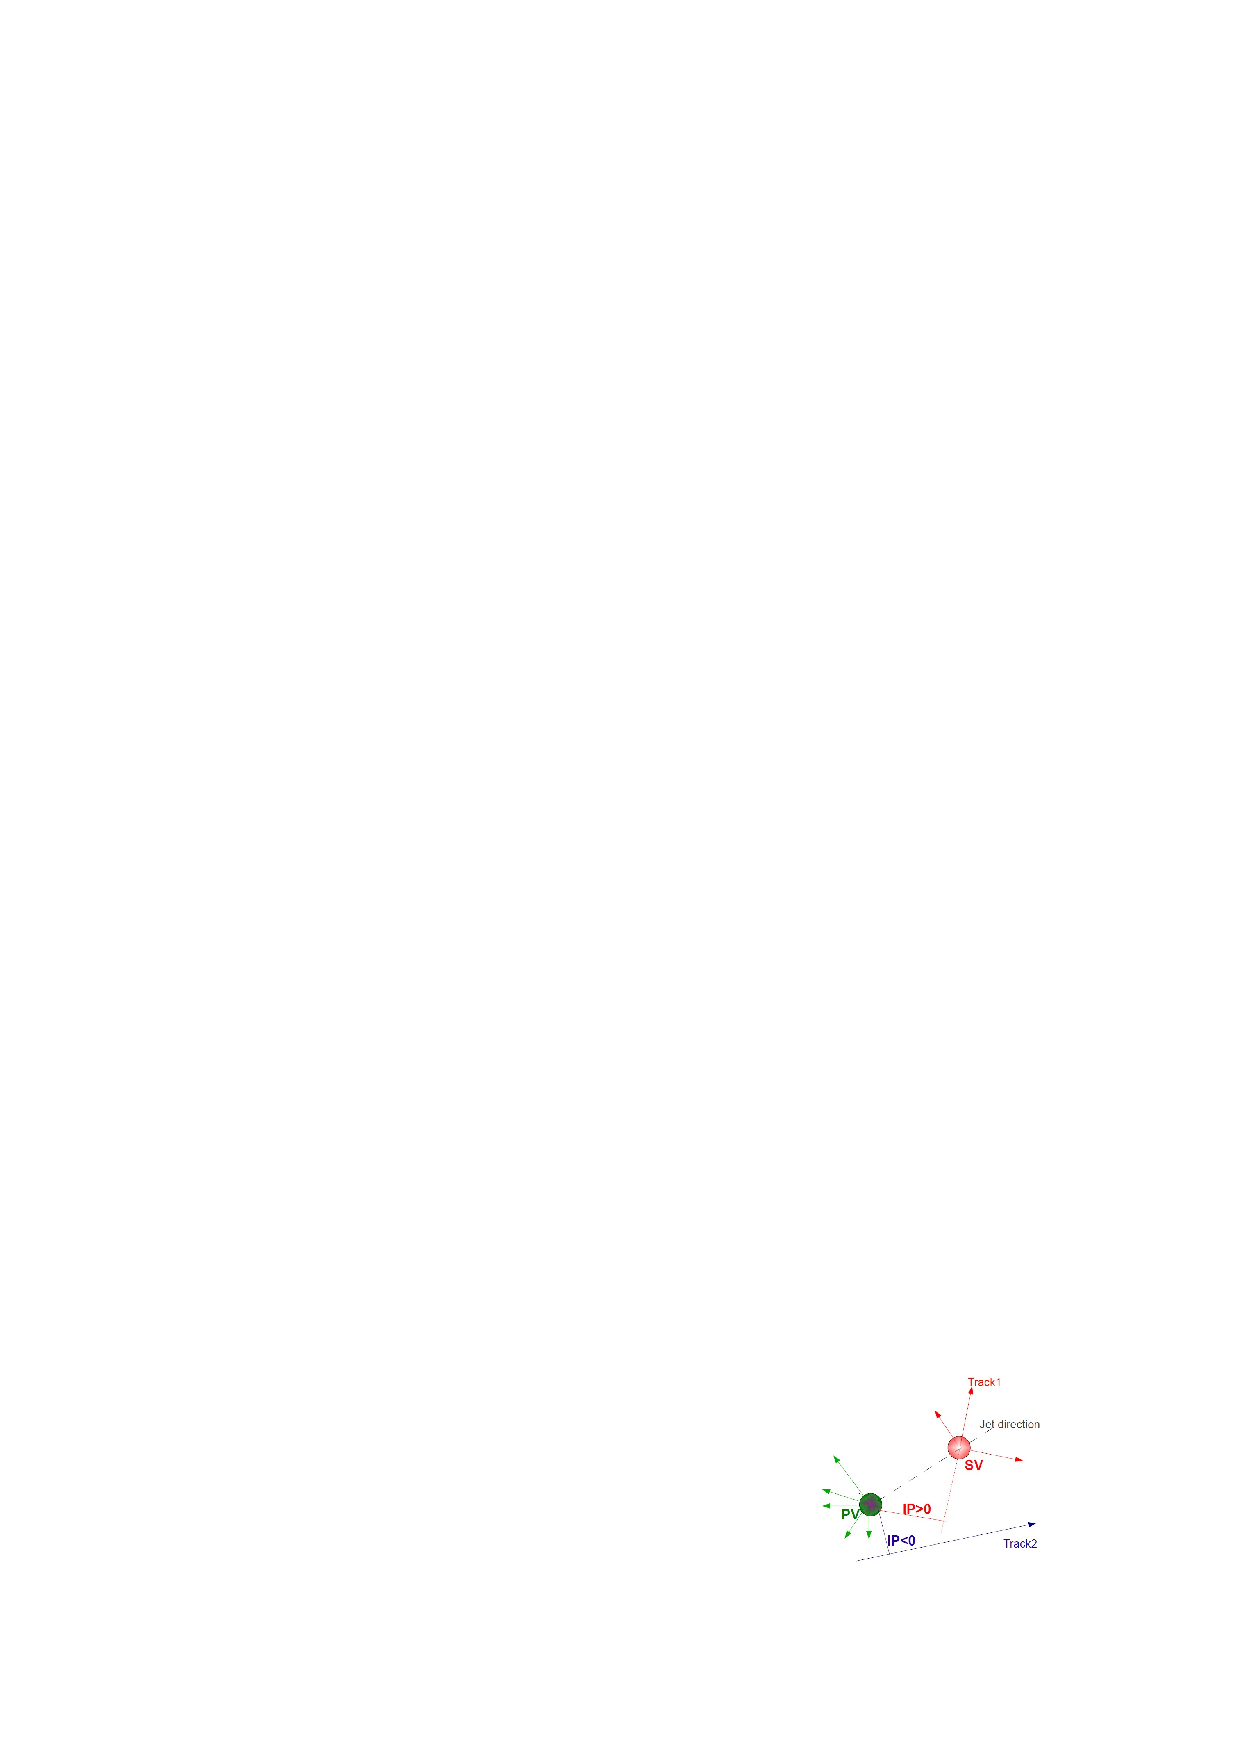
\includegraphics[width=0.50\linewidth]{Image/bCSV.pdf}
\caption{ Primary and secondary vertex with tracks and impact parameter. IP $> 0$ or $< 0$ if tracks
are upstream or downstream along the jet direction. This figure is taken from Ref.~\cite{Ferro:2012tg}.} 
\label{fig:bCSV}
\end{figure}

\subsection{Track Selection}
\label{ss:Track Selection}
The tracks are selected with the criteria listed in Table~\ref{tab:track_sel}.
These requirements ensure the tracks are closer to the PV and not coming from pileup vertices.
After track selection, the SV is reconstructed.
\begin{table}
  \caption{Track selection criteria. PCA stands for the point of closest approach.}
 \begin{center}
 \begin{tabular}{cc}\hline\hline
 Variable & Selection \\ \hline\hline
 $\pt$ associated with tracks & $>0.8$ GeV \\
 number of hits associated with tracks in the tracker & $>8$ \\
 longitudinal component of IP & $< 0.3$~\unit{cm}\\
 distance between PCA of tracks from the PV and jet-axis & $<0.07$~\unit{cm}\\
 distance between PCA of tracks from the jet-axis and PV & $< 5$~\unit{cm}\\
 the displaced track should have & IP $>50$~\unit{$\mu$m} and $\frac{\rm IP}{\sigma_{\rm IP}}>1.2$\\\hline
 \end{tabular}
 \end{center}
 \label{tab:track_sel}
 \end{table}

\subsection{Reconstruction of Secondary Vertex}
For Run-I, the {\em combined secondary vertex (CSV)} method used the adaptive vertex
reconstruction algorithm~\cite{Waltenberger:1166320}, which is based on adaptive vertex
fitter~\cite{Fruhwirth:1027031} to reconstruct the SV.
On the other hand, in case of Run-II, the CSVv2 uses the inclusive vertex finder (IVF)
algorithm~\cite{Khachatryan:2011wq} for the same purpose.
The collection of selected tracks are used as inputs to the IVF. The displaced tracks are used as seed.
The cluster of tracks is formed from seed track depending on the angles and distance between them.
The adaptive vertex fitter is used to fit the clusters.
The selection listed in Table~\ref{tab:sv_sel} are applied for the SV.
\begin{table}
  \caption{Secondary vertex selection criteria. $d_{\rm PV, SV}^{\rm trans}$ is the 2D flight
  distance or the distance between a primary and secondary vertex in the transverse plane.}
 \begin{center}
 \begin{tabular}{cc}\hline\hline
 Variable & selection \\ \hline\hline
     number of tracks associated with the SV & $>$ 2 \\
     $d_{\rm PV, SV}^{\rm trans}$ & $>$ 0.1~\unit{mm} \\
     $d_{\rm PV, SV}^{\rm trans}$ & $<$ 2.5~\unit{cm} \\
     mass associated with the SV & $<$ 6.5 GeV\\
     $\Delta R$ (jet axis, secondary flight direction) & $<$ 0.4\\ \hline
 \end{tabular}
 \end{center}
 \label{tab:sv_sel}
 \end{table}

\subsection{Multi-layer Perceptron Training}
Three types of discriminating variable, as shown below, are used in multi-layer perceptron training to identify the secondary vertex.
\begin{itemize}
    \item category-I: jet with $N_{\rm SV} > 1$,
    \item category-II: jet with pseudo-vertex~\cite{CMS-PAS-BTV-15-001}, and
    \item category-III: jet with no SV or no pseudo-vertex.
\end{itemize}
The discriminating variables from the vertex-categories are combined using a likelihood ratio,
which gives the b-discriminator value.
The b-discriminator value for the \mujets and \ejets channel is shown in
Figure~\ref{fig:pfCISV_lepBTag}.
There are three official b-tag working points: {\em loose}, {\em medium}, and {\em tight} with
b-tag efficiency [defined in Eq.~(\ref{eq:btag_eff})] 81\%, 63\%, and 41\%, respectively.
The corresponding probability of a light jet being misidentified as a b-jet is 10\%, 1\%, and 0.1\%.
In this analysis, we use the medium working point i.e., b-discriminator $>$ 0.8484 for b-tagging.
The efficiency of all b-taggers for b, c, and light-quarks are shown in Table (\ref{tab:bTagEff}). 
\begin{table}
\begin{center}
\caption{The efficiency of loose, medium, and tight b-tag working points for different quark-flavor
    of jets \cite{Sirunyan:2017ezt}. These efficiencies are calculated from
\ttbar events with jet \pt $>$ 20 GeV.}
\begin{tabular}{cccccc}
\hline
\hline
WP & $\epsilon^b$ (\%) & $\epsilon^c$ (\%) & $\epsilon^{udsg}$ (\%)& CSVv2 \\ \hline\hline
b-tagger L & 81 & 37 & 8.9 & $>$ 0.5426  \\
b-tagger M & 63 & 12 & 0.9 & $>$ 0.8484   \\
b-tagger T & 41 & 2.2& 0.1 & $>$ 0.9535   \\
\hline
\end{tabular}
\label{tab:bTagEff}
\end{center}
\end{table}

\begin{center}
\begin{figure}
\subfigure[b-jet discriminator for the \mujets channel]{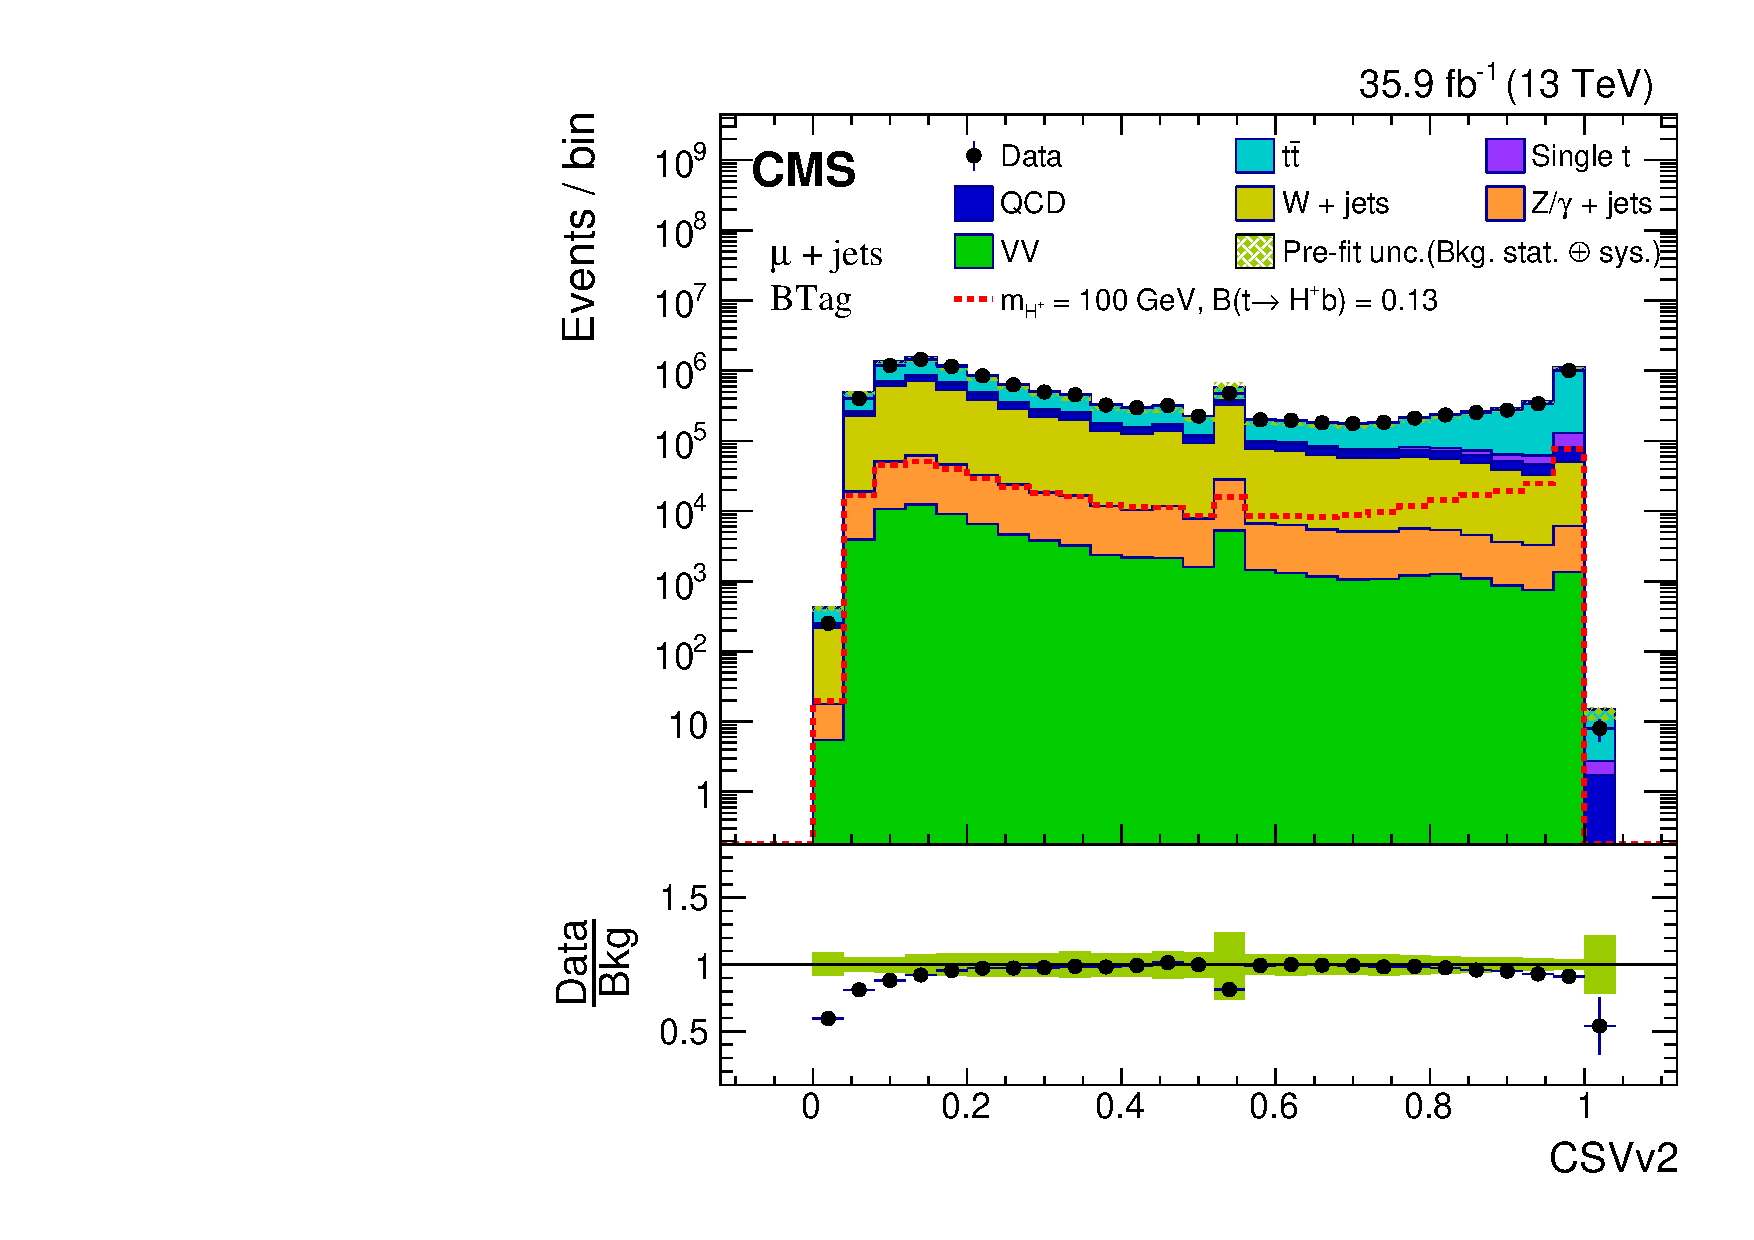
\includegraphics[width=0.50\linewidth]{Image/Muon/BTag/pfCISV_muBTag.pdf}}
\subfigure[b-jet discriminator for the \ejets channel]{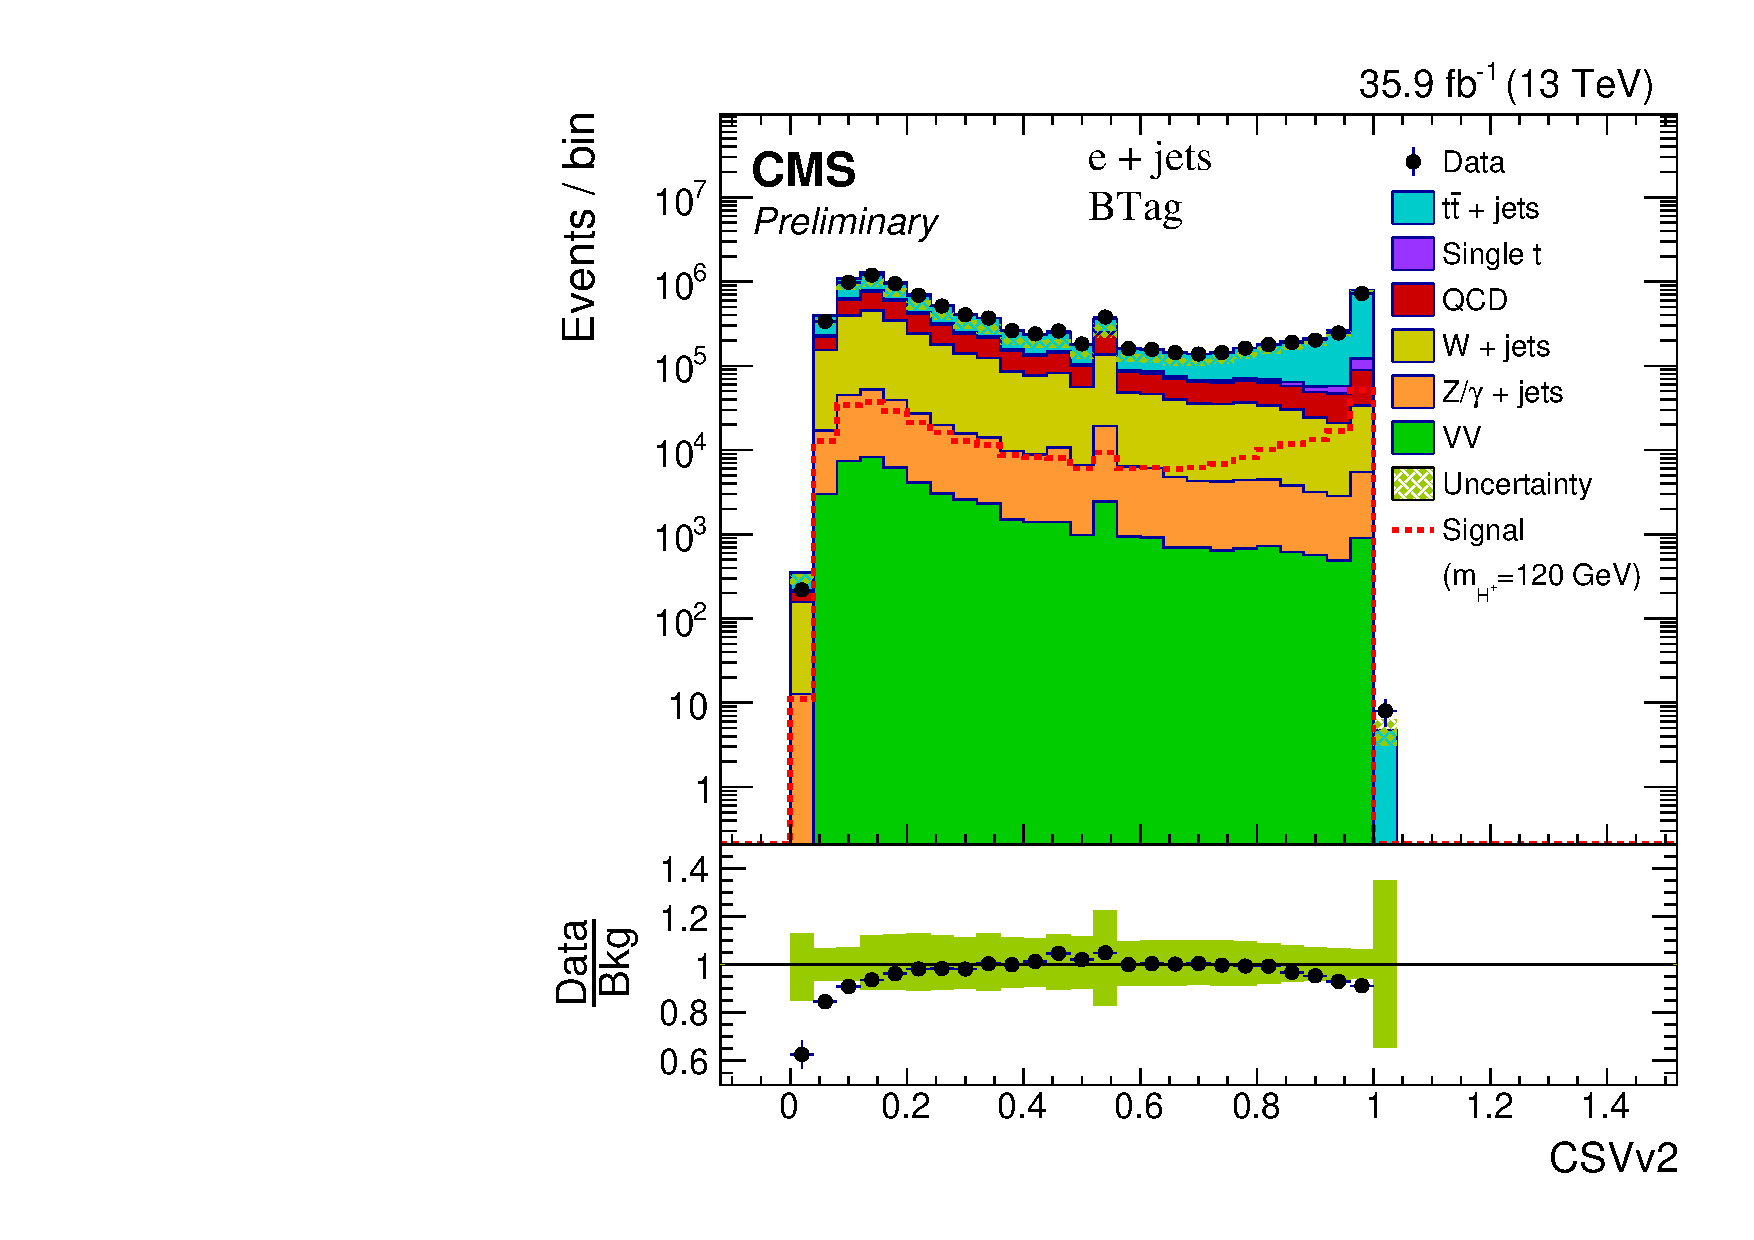
\includegraphics[width=0.50\linewidth]{Image/Electron/BTag/pfCISV_eleBTag.pdf}}
\caption{The b-discriminator distributions of all jets, after $N_{jets} \geq 4$ selection as described in Sec.~\ref{s:secEvtSel}, obtained using CSVv2 method for the \mujets and \ejets channel.}
\label{fig:pfCISV_lepBTag}
\end{figure}
\end{center}



%-------------------------------------
% KinFit Fitting
%-------------------------------------
\section{Kinematic fit}
\label{s:KinFit}

In this analysis, the charged Higgs boson is decaying to the \PQc and $\bar{\PQs}$ 
quark. The invariant mass of the \PQc$\bar{\PQs}$ system ($\mjj$) is thus used as the 
final observable. The $\mjj$ distribution of two highest \pt, non \PQb jets is
shown in Figures~\ref{subfig:mjj_muBTag} and \ref{subfig:mjj_eleBTag} for
both channels. For the true semileptonic \ttbar events, the mean of the $\mjj$ distribution 
should be close to 80 \GeV, which is the mass of the \PW boson. However, the mean of
$\mjj$, as shown in Figures~\ref{subfig:mjj_muBTag} and \ref{subfig:mjj_eleBTag},
is about 128 \GeV because the two light jets in every event may not necessarily 
come from the decay of a \PW boson. Secondly, the $\mjj$ distribution has a long tail 
which might constrain the search for new resonances in the dijet mode. 
\begin{figure}
    \centering
    \subfigure[With reconstructed jets after \PQb jet selection \label{subfig:mjj_muBTag}]
    {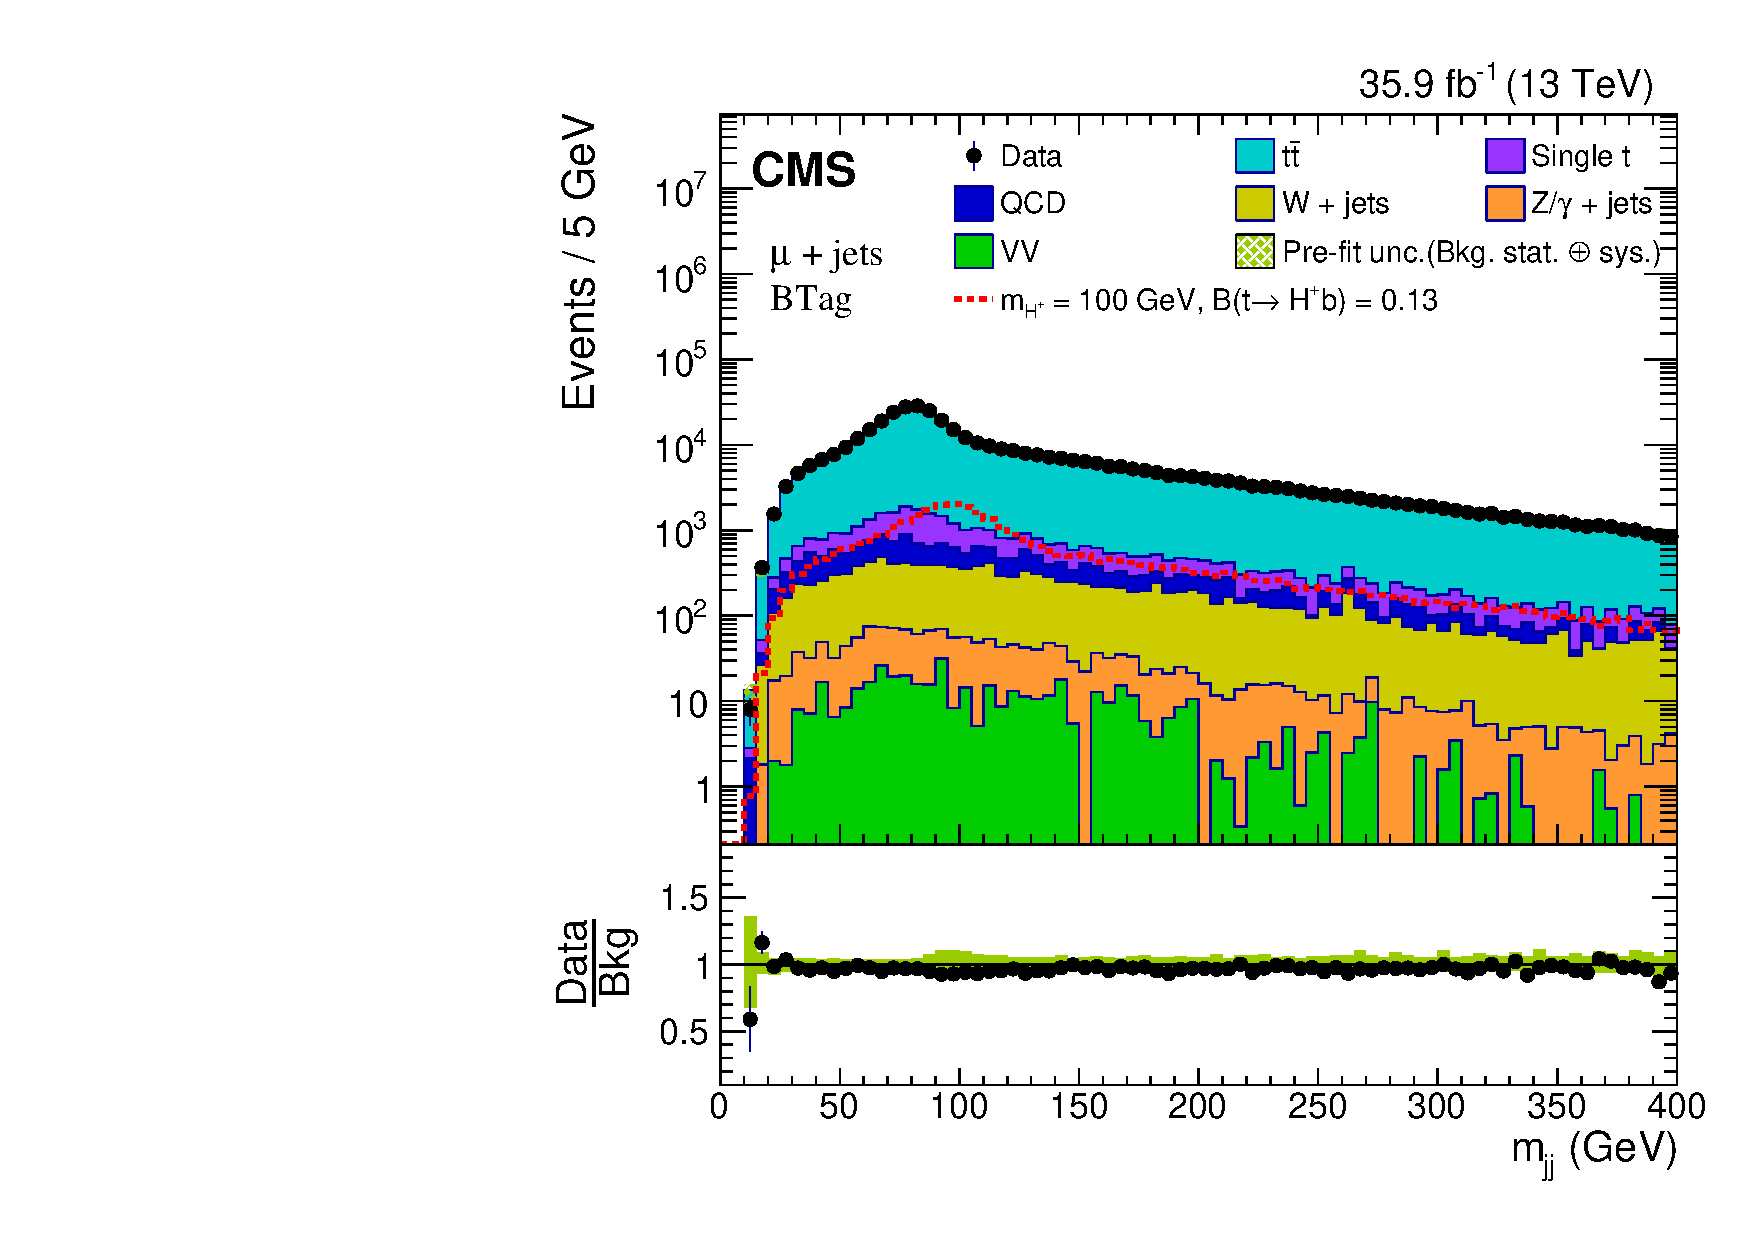
\includegraphics[width=0.49\linewidth]{Image/Muon/BTag/mjj_muBTag.pdf}}
    \subfigure[With reconstructed jets after \PQb jet selection \label{subfig:mjj_eleBTag}]
    {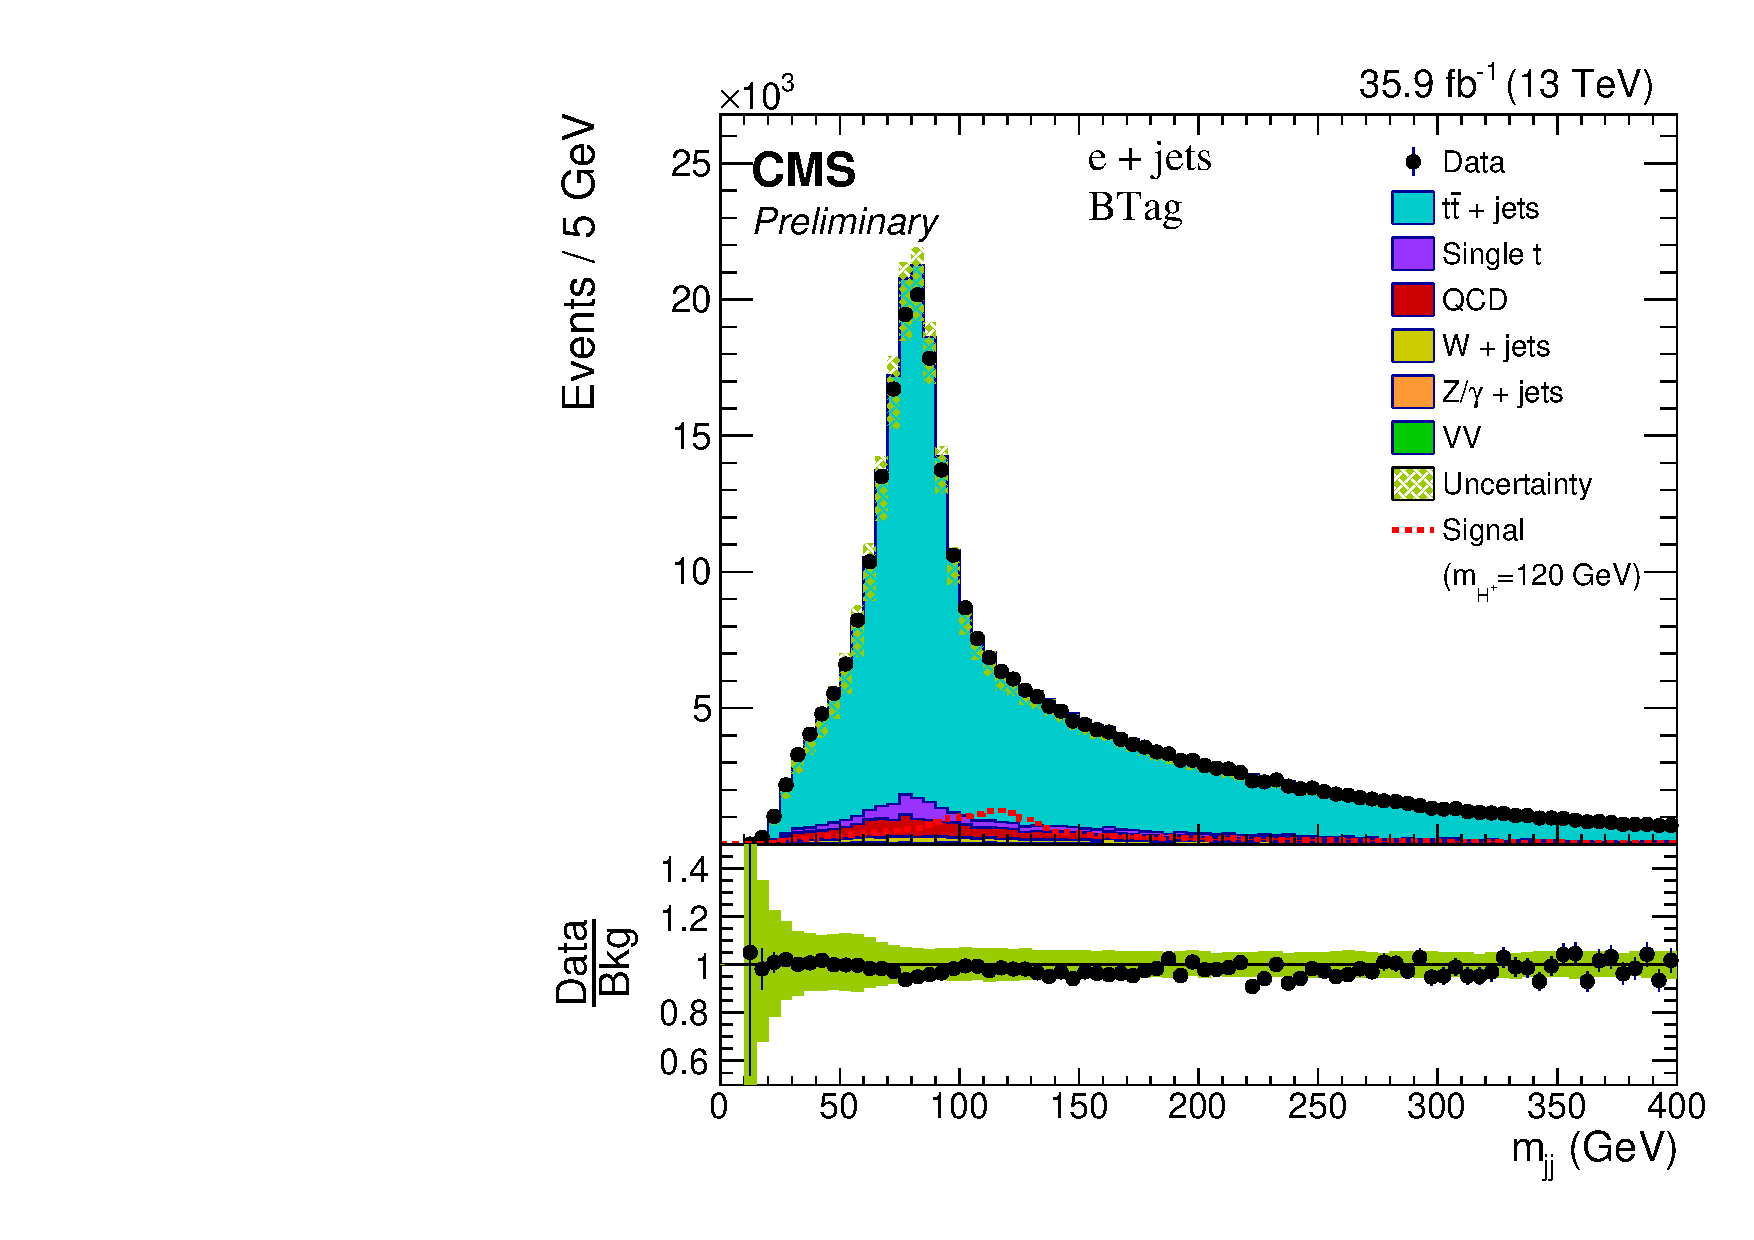
\includegraphics[width=0.49\linewidth]{Image/Electron/BTag/mjj_eleBTag.pdf}}
    \vfil
    \subfigure[With kinematic fitted jets after KF selection \label{subfig:mjj_kfit_muKinFit}]
    {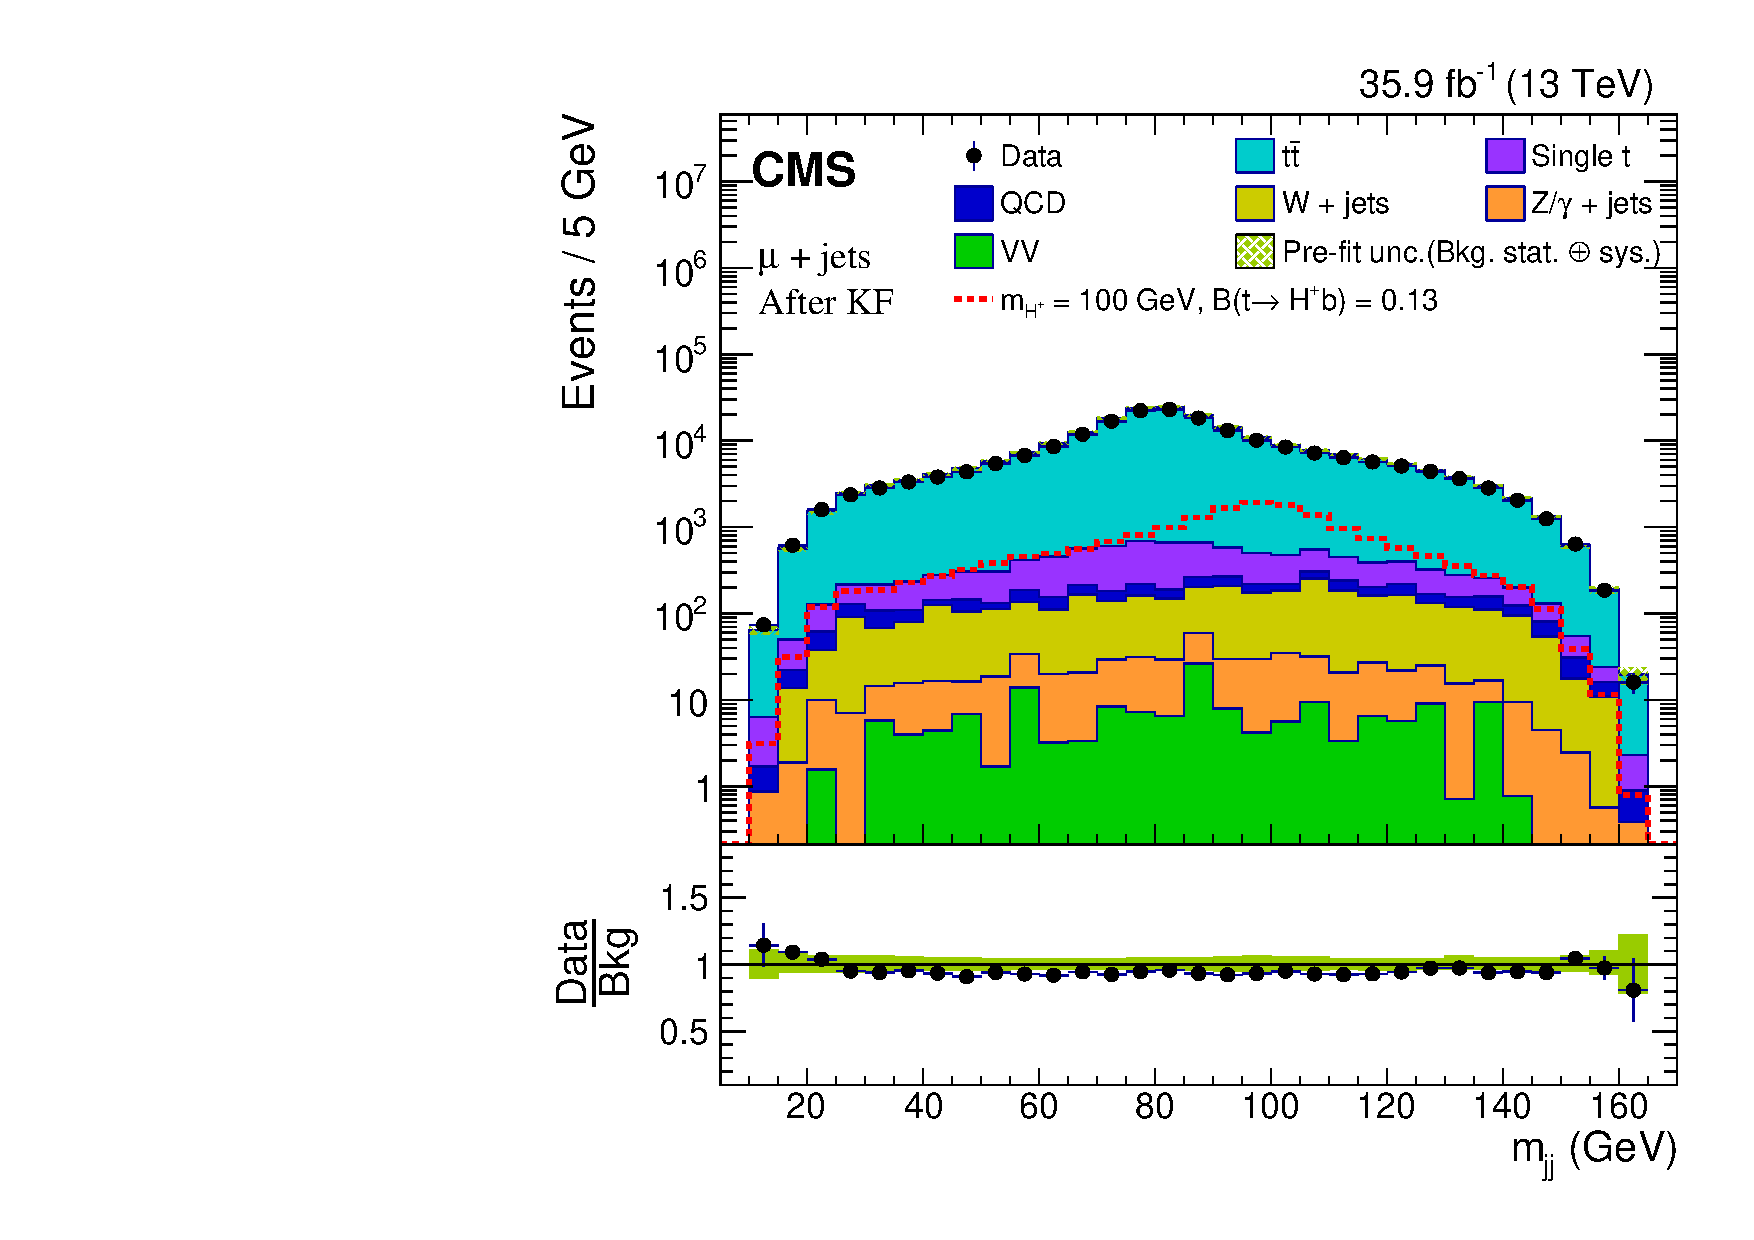
\includegraphics[width=0.49\linewidth]{Image/Muon/KinFit/mjj_kfit_muKinFit.pdf}}
    \subfigure[With kinematic fitted jets after KF selection \label{subfig:mjj_kfit_eleKinFit}]
    {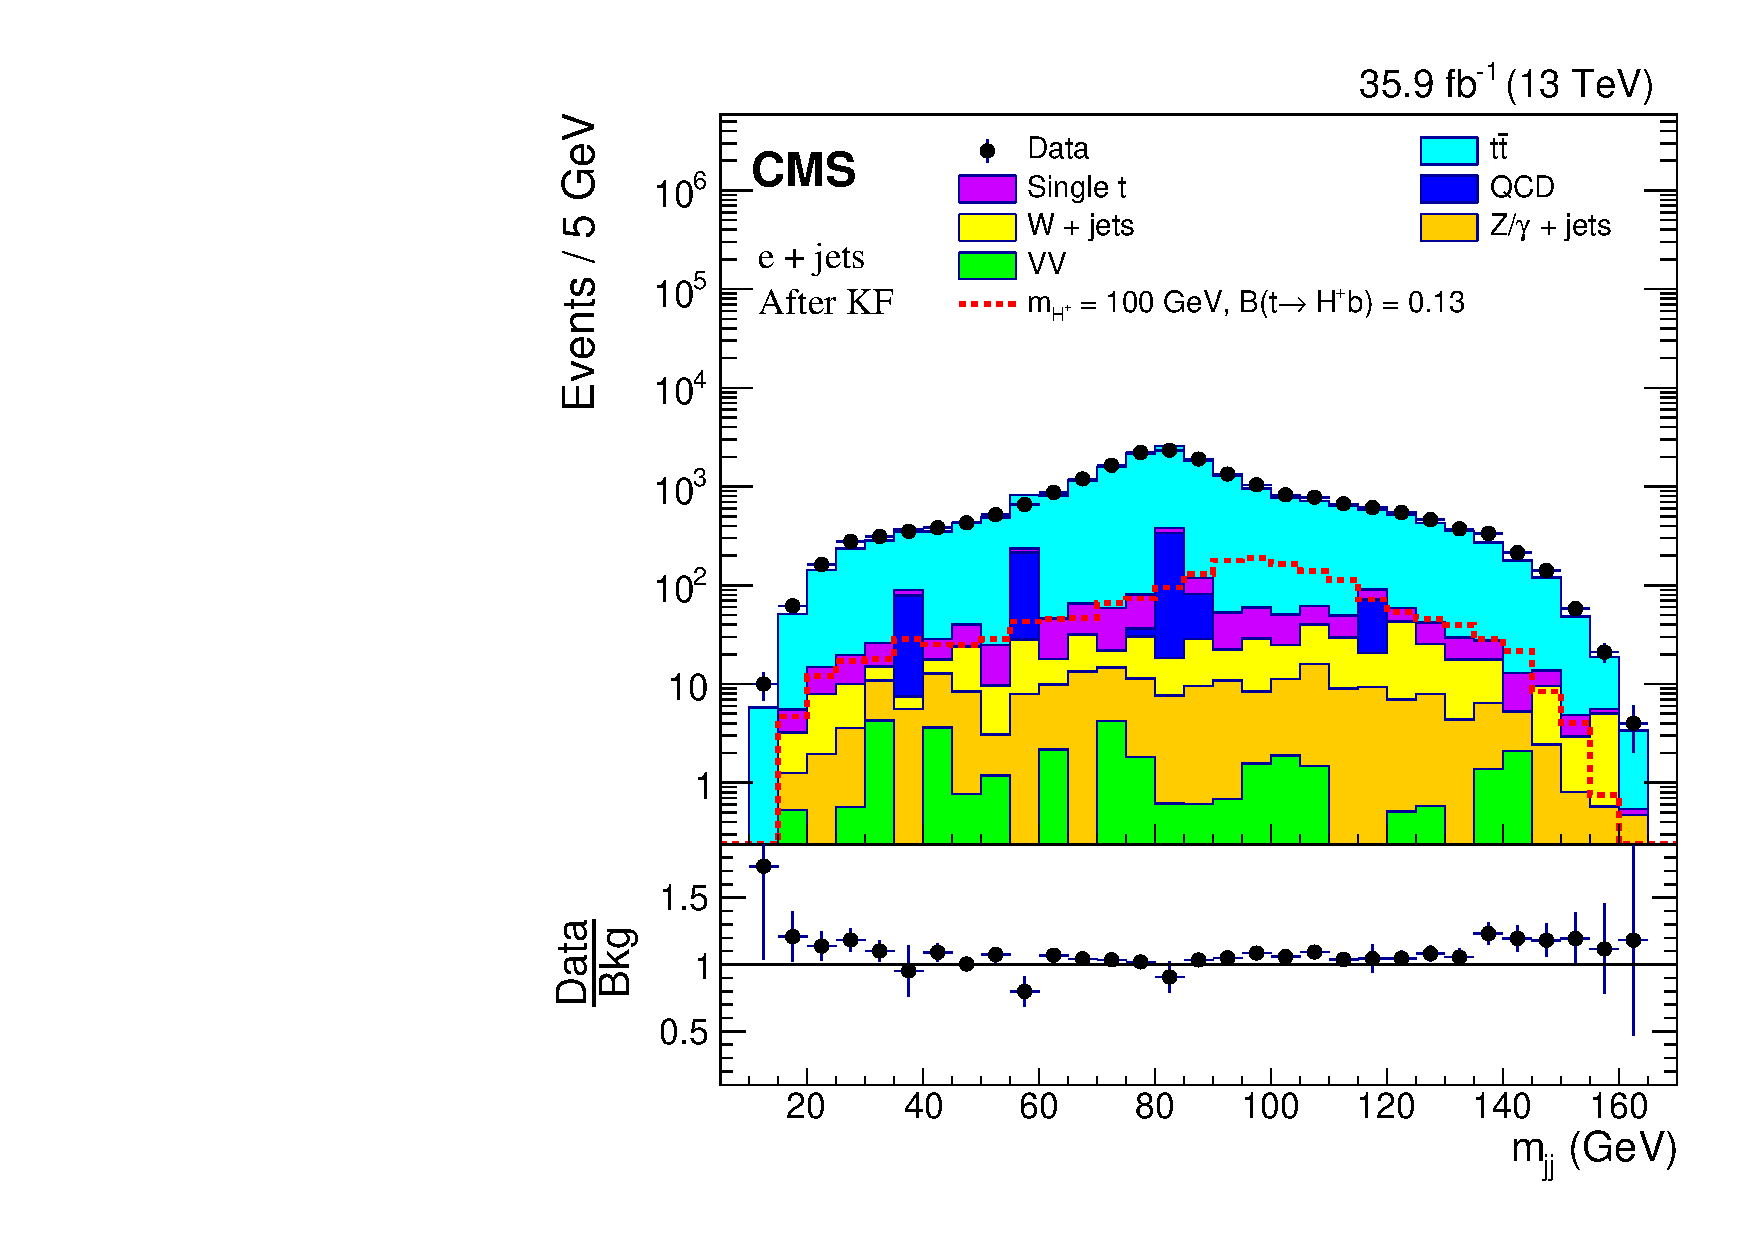
\includegraphics[width=0.49\linewidth]{Image/Electron/KinFit/mjj_kfit_eleKinFit.pdf}}
    \caption{$\mjj$ distributions of two non \PQb, highest \pt jets for the 
     \mujets and \ejets channel. The distributions of 
     Figures~\ref{subfig:mjj_muBTag} and \ref{subfig:mjj_eleBTag} are obtained 
     using reconstructed jets after applying \PQb tag scale factor as described 
     in Section~\ref{s:secEvtSel}. On the other hand, the distributions of 
     Figures~\ref{subfig:mjj_kfit_muKinFit} and \ref{subfig:mjj_kfit_eleKinFit} 
     are calculated using kinematic fitted jets after kinematic fit selection. 
     The mean of the invariant mass distribution from kinematic fitted jets 
     is closer to the \PW mass as compared to that of reconstructed jets.}
    \label{fig:mjjBTagKinFit}
\end{figure}

To select true semileptonic \ttbar events, a kinematic fit is performed on the 
reconstructed objects using the top kinematic fitter package~\cite{DHondt:2006iej}. 
The \verb|TopKinFitter| takes physics objects such as lepton, jets, \MET, and their 
resolutions as input, and gives improved four-vectors of lepton, jets, and neutrino with 
associated $\chi^2$ and probability of the fit as output. It constrains the reconstructed 
\PQt quark mass to its nominal value (\mt = 172.5 \GeV). In the output, the 
\verb|TopKinFitter| gives only four jets (2 \PQb jets from leptonic and hadronic modes, and 2 
light jets from hadronic mode), 1 lepton, and neutrino. It also separates jets coming from
leptonic and hadronic decay modes of \ttbar. The 2 light jets coming from hadronic 
decay mode are further used for \PQc tagging as described in Section~\ref{s:cTag}. 
A more detailed description of the kinematic fitting is given below.

\section{Input to the TopKinFitter}
\label{ss:inputKF} 
After applying selection criteria on physics objects as described
in Section~\ref{s:secEvtSel}, the event which is passed to the \verb|TopKinFitter| contains 
only one lepton, \MET and at least 4 jets. The \PQb discriminator value with the medium 
working point is also given as the input to the \verb|TopKinFitter| to separate \PQb jet 
from light jets (more details in Section~\ref{ss:jetSepKF}). The constraints on the \ttbar 
system along with the theoretical mass of the \PQt quark are also specified
(more details in Section~\ref{ss:constraintKF}). All the constraints and invariant mass are 
parameterized in terms of $E_{T}$, $\eta$, and $\phi$ variables of the physics objects. 
The components of 4-momentum vector in terms of these variables are given as
\begin{equation}
E = E_{T} \sin\theta, p_x = E_{T}\cos\phi, p_y = E_{T}\sin\phi, p_z = E_{T}\cot\theta,
\end{equation}
and the invariant mass of two particles, in the relativistic limit, is given by
\begin{equation}
	m_{\rm{inv}} = \sqrt{2 E_{T_1}E_{T_2}\left(\cosh(\eta_1 - \eta_2) - \cos(\phi_1 - \phi_2)\right)}
\end{equation}
where $\eta = \ln\cot(\theta/2)$. The resolution of each physics object as a function of 
\pt and $\eta$, and the JER scale factors from different $\eta$ binning are also given in the 
input. Apart from the physics objects, various inputs related to the minimization of 
$\chi^2$ such as the maximum number of iterations, criteria on the convergence of the $\chi^2$
are also specified (more details in Section~\ref{ss:chi2KF}).

\section{Separation of jets}
\label{ss:jetSepKF} 
For the semileptonic decay mode of the \ttbar, the first step is to separate 2 
\PQb jets from light jets and the second step is to identify each \PQb jet from hadronic 
and leptonic modes.  All the jets are sorted in their \pt order and first 4 jets are
selected. To find out the two \PQb jets, a \PQb tag probability is calculated using 
following formula \cite{DHondt:2006iej}
\begin{equation}
	L_{b}(x) = \frac{\text{PDF}_b(x)}{\sum_{i=1}^5 \text{PDF}_i(x)}
\end{equation}
Where $\text{PDF}_i(x)$ is the probability distribution function of \PQb discriminator value
(x) for flavour $i$. An event is selected if two jets have \PQb tag probability of more 
than 60\%. The jet-parton matching is also performed for each jet. For n number of 
jets, there are exactly n number of partons. The number of permutations in the 
jet-parton matching is given by
\begin{equation}
	N_{\rm{permutations}} = \frac{n!}{(n-4)!}
\end{equation}
Therefore for 4 jets, there are 24 permutations. All the 24 permutations are shown 
in \cite{KinFitThesis} through diagrams. However, after identifying two \PQb jets, the number of 
permutations reduces to 12 as the two \PQb jets are interchangeable. For each 
jet-parton permutation, a $\chi^2$ is constructed, as described in Section
\ref{ss:chi2KF}, and the permutation with the lowest value of $\chi^2$ is
treated as the correct matching. Afterward, three jets (1 \PQb jet and 2 light jets) 
have to be selected to form hadronic decaying \PQt quark. For this, several sensitive 
variables are used \cite{DHondt:2006iej} such as the angle between jets and lepton, 
angular separation between the generated and reconstructed jets, etc.

\section{Kinematic constraints}
\label{ss:constraintKF} 
The semileptonic decay mode of the \ttbar has 4 jets, 1 lepton and the neutrino in 
the final state. The x and y-component of the neutrino are taken from the \MET, as the 
missing transverse energy is attributed to the neutrino. And the z-component of the 
neutrino, $p^v_z$, is determined from the fit. The following kinematic constraints are 
imposed on the semileptonic \ttbar system
\begin{subequations}
\begin{eqnarray}
	m_{\rm{inv}}(b^{\text{had}}q\bar{q}) = m_{t} = 172.5 \text{\GeV} \label{eq:constraintKF1}\\
	m_{\rm{inv}}(b^{\text{lep}}l\nu_l)   = m_{\bar{t}} = 172.5 \text{\GeV} \label{eq:constraintKF2}
\end{eqnarray}
\label{eq:constraintKF}
\end{subequations}
After the fit, the $p^v_z$ is determined from the Equation (\ref{eq:constraintKF2}). 
For every event, a $\chi^2$ is constructed as discussed in Section~\ref{ss:chi2KF}.
The $\chi^2$ is minimized by varying \pt, $\eta$, and $\phi$ of each object within
their resolution. Those values of \pt, $\eta$, and $\phi$ variables are finally selected 
which minimises the $\chi^2$ and at the same time satisfies Equation (\ref{eq:constraintKF}).

\section{$\chi^2$ of the fit}
\label{ss:chi2KF} 
For every selected event, a $\chi^2$ is constructed which is given by
\begin{equation}
	\chi^2 = \left(\frac{m_t - 172.5}{\sigma_{m_{t}}}\right)^2 + 
	\left(\frac{m_{\bar{t}} - 172.5}{\sigma_{m_{\bar{t}}}}\right)^2+
	\sum_{i}\left(\frac{p_i^{\text{fit, lep}} - p_i^{\text{lep}}}{\sigma_{p^{\text{lep}}_i}}\right)^2+
	\sum_{j}\sum_{i}\left(\frac{p_i^{\text{fit}, \text{jet}_j} - 
	p_i^{\text{jet}_j}}{\sigma_{p^{\text{jet}_j}_i}}\right)^2
\label{eq:chi2KF}
\end{equation}
where $\sigma_{m_{t}}$ is the resolution of the mass of the \PQt quark and $\sigma_{p_{i}}$ 
is the momentum resolution of three component ($i= 1, 2, 3$) of the corresponding lepton and jets.
The $p^{\text{fit}}$ is the fitted momentum of the given lepton and jets. The $\chi^2$, given in 
Equation (\ref{eq:chi2KF}), is minimized using the Lagrangian multipliers under the constraints 
given in Equation (\ref{eq:constraintKF}). A detailed mathematical description for the minimization 
of the $\chi^2$ is given in \cite{DHondt:2006iej}. The $\chi^2$ is minimized iteratively where in 
each step the 4 components of the momentum vector of each object are varied
within their resolution and a $\chi^2$ and the constraint is calculated. The
fit is declared to be converged if the following constraints are satisfied
\begin{subequations}
\begin{eqnarray}
	\frac{\chi^2 (n-1) - \chi^2 (n)}{\text{ndf}} < \epsilon_{\chi}\\ 
	m_{\rm{inv}}(b^{\text{had}}q\bar{q}) - 172.5 < \epsilon_{c}\\
        m_{\rm{inv}}(b^{\text{lep}}l\nu_l) - 172.5 < \epsilon_{c}
\end{eqnarray}
\end{subequations}
where $\epsilon_{\chi} = 5\times 10^{-05}$, $\epsilon_{c} = 0.0001$, and \text{ndf}
is the number of degrees of freedom which is equal to 1 as we have two 
constraints and one free parameter ($p_z^\nu$). The total number of iterations ($n$)
is 500.

\section{Output of the TopKinFitter}
\label{ss:outputKF} 
For every event, the \verb|TopKinFitter| gives the status of fit which is 0 if 
the fit converged and 1 if it did not, $\chi^2$ of the fit, probability ($P_{\chi}$) 
of the goodness-of-fit of $\chi^2$, and the 4 momentum vector of physics objects such
as jets, lepton and a neutrino. The $\chi^2$ and $P_{\chi}$ are related by the 
following equation
\begin{equation}
	P_{\chi} = \exp(\frac{-\chi^2}{2})
\end{equation}
The fit also separates jets from hadronic and leptonic decay mode of \ttbar, 
that is, it gives one hadronic \PQb jet, one leptonic \PQb jet, and 2 light jets from hadronic
decay modes. The \PQc tagging criteria are applied further on the 2 light jets as 
discussed in Section \ref{s:cTag}. The $\mjj$ distribution of the light jets is used in 
further analysis.

\section{Selection and performance}
\label{ss:selKF} 
Due to wrong jet combinatorics, the fit does not converge for every event. Only 
those events are selected for which the fit converges. The efficiency of fit convergence 
is 73\% for simulated \ttbar sample and 71\% for data for both channels.
Further, the angular separation between reconstructed and kinematic fitted 
lepton and jets are required to be less than 0.2 to make sure that they are almost in the same
direction. The same $\Delta \rm R$ cut is applied on reconstructed and kinematic
fitted jets. Also, the \pt cut on kinematic fitted lepton and jets are required to
be the same as that on the reconstructed jets and lepton. After applying these additional 
cuts on $\Delta \rm R$ and \pt, the kinematic fit efficiency reduces to 47\% for \ttbar 
and 44\% for data for both channels. In summary, the following kinematic fit selections are applied: 
\begin{itemize}[leftmargin=*]
 \item fit is converged,
 \item $\Delta \rm R (\text{fitted lepton, reconstructed lepton}) < 0.2$,
 \item $\Delta \rm R (\text{fitted jet, reconstructed jet}) < 0.2$%, and
% \item $\chi^2_{kfit} >0$, $Prob_{kfit} > 0$.
\end{itemize}
Event yields after kinematic fit selections are shown in the 7th column of Tables~\ref{tab:cutflow_mu},
\ref{tab:cutflow_ele}, \ref{tab:cutflow_mu_sig} and \ref{tab:cutflow_ele_sig}.
From these tables, we see that almost half the number of events is reduced after these selections. 
The $\mjj$ distribution from the two light jets after kinematic fit selection is shown in 
Figures~\ref{subfig:mjj_kfit_muKinFit} and \ref{subfig:mjj_kfit_eleKinFit} for both channels. 
The mean of these distributions is 84\GeV which is close to the mass of \PW boson. 

The kinematic fit is also performed after applying jet energy corrections such as JES and JER.
For up and down systematics of JES and JER, the fit is performed separately 
on every event after correcting jet \pt using the corresponding scale factors.
The output of the fit for each systematic is stored in a different collection
using the \verb|EDProducer|. The kinematic fitting is a time-consuming process 
which takes, on average 0.002 seconds per event for \ttbar process. Therefore, 
performing all (nominal, \verb|JESup|, \verb|JESdown|, \verb|JERup|, and 
\verb|JERdown|) the kinematic fitting takes a reasonable amount of time.

\section{Comparison of data and background after kinematic fitting}
\label{s:secCPlotsKF}

Data to background comparison of variables from the kinematic fitted objects after kinematic 
fit selection are shown in Figures~\ref{fig:kfitPlot1},~\ref{fig:kfitPlot2}, and~\ref{fig:kfitPlot3}. 
There is also a good agreement between data and simulation within the statistical and systematic 
uncertainties. Here also we see a similar disagreement for the higher value of \pt and \MET as
we have after \PQb jet selection described in Section~\ref{s:secEvtSel}.

%After KinFit: Pt_lep, Eta_lep, Pt_jets
\begin{figure}
    \centering  
    \subfigure[\pt of muon]{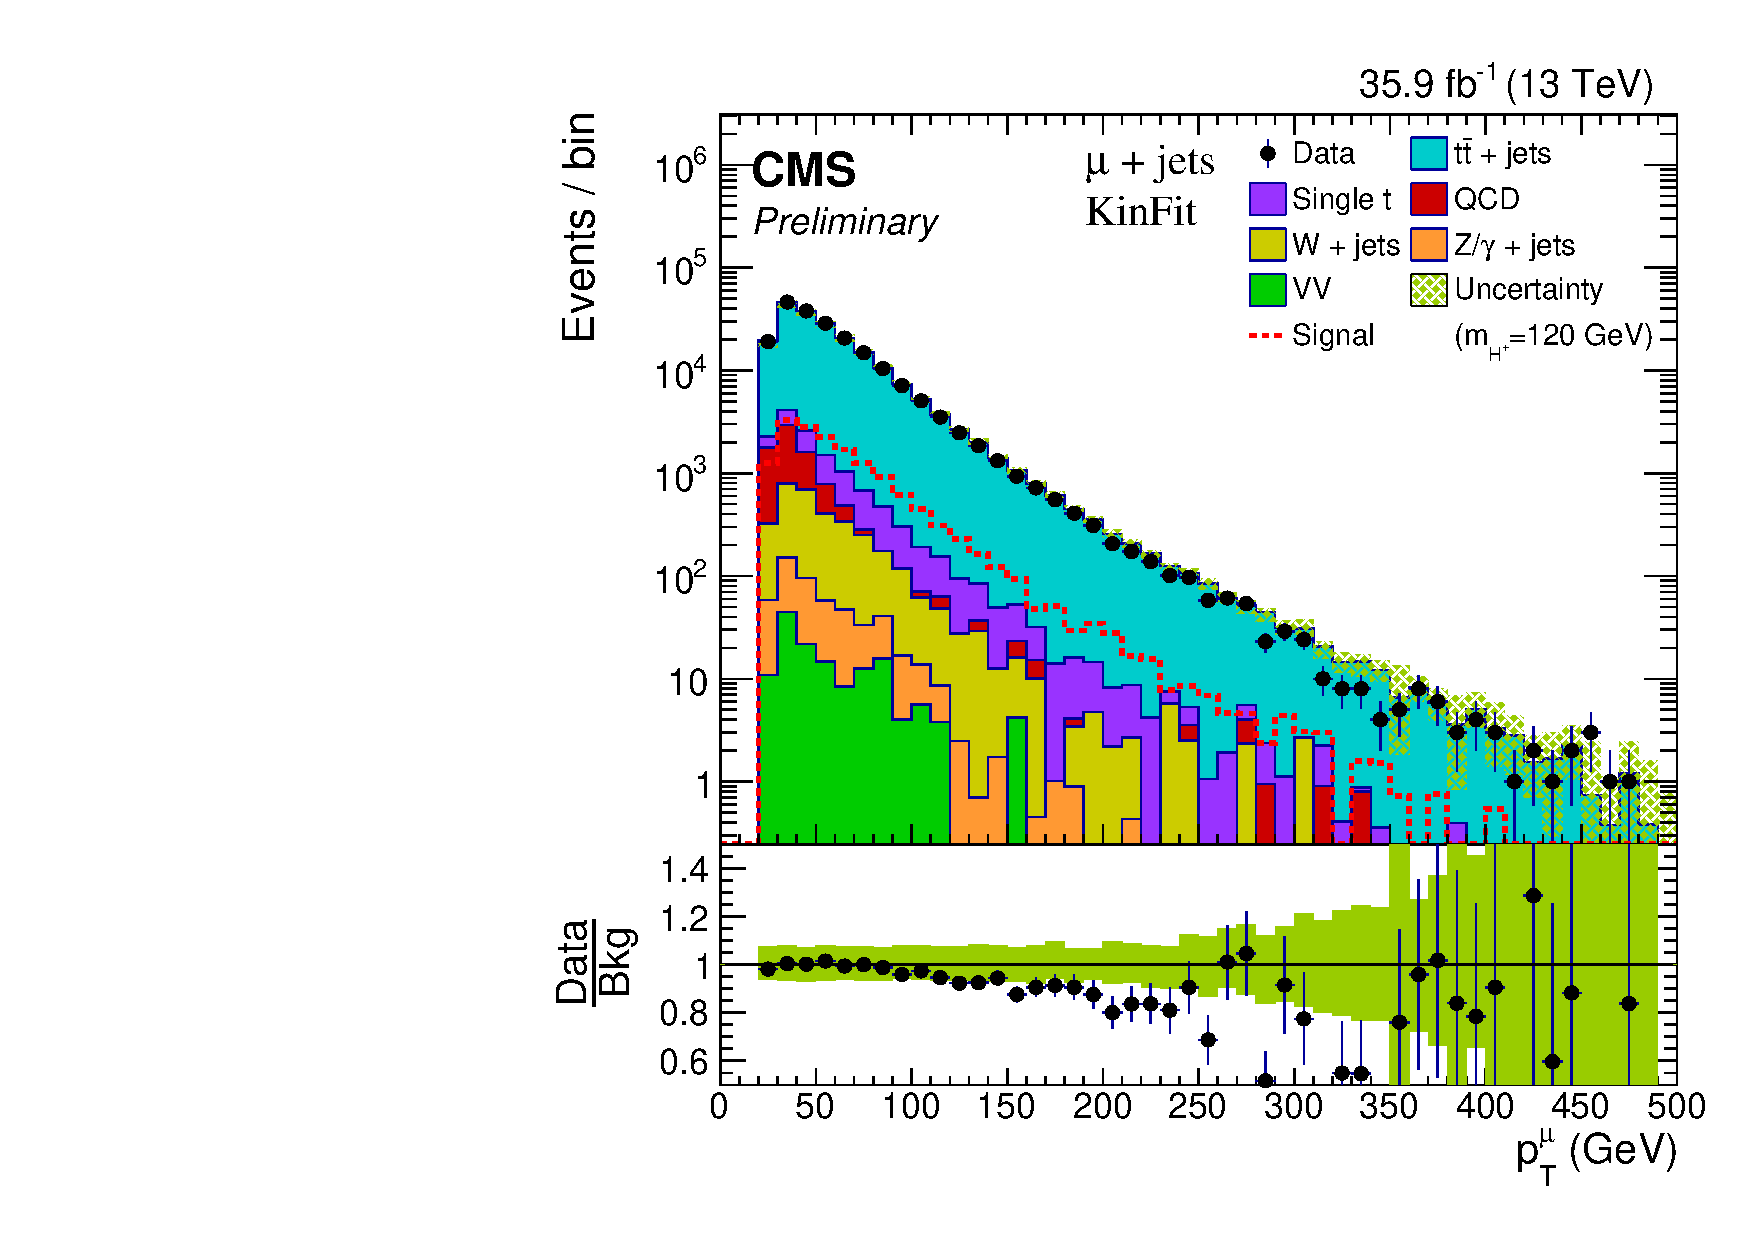
\includegraphics[width=0.40\linewidth]{Image/Muon/KinFit/pt_mu_muKinFit.pdf}}
    \subfigure[\pt of electron]{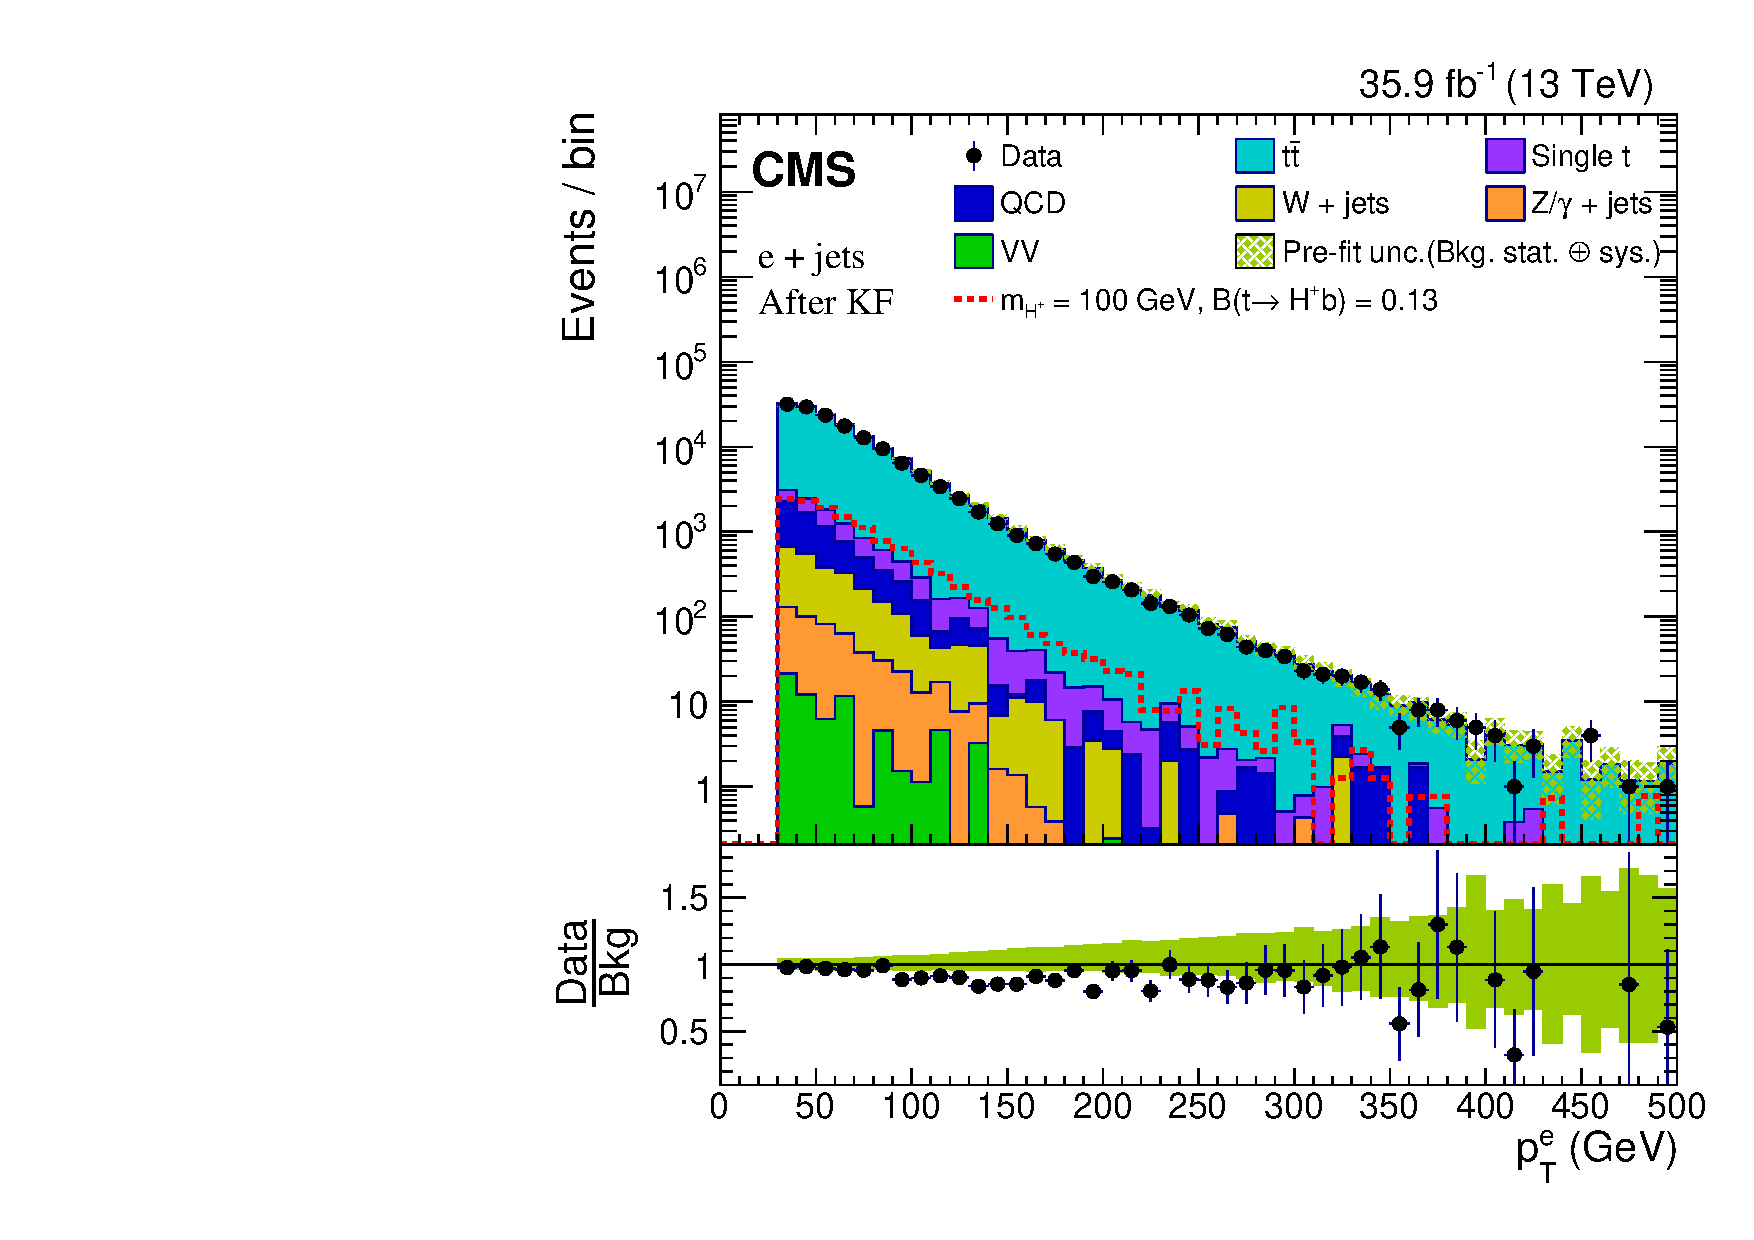
\includegraphics[width=0.40\linewidth]{Image/Electron/KinFit/pt_ele_eleKinFit.pdf}}
    \vfil
    \subfigure[$\eta$ of muon]{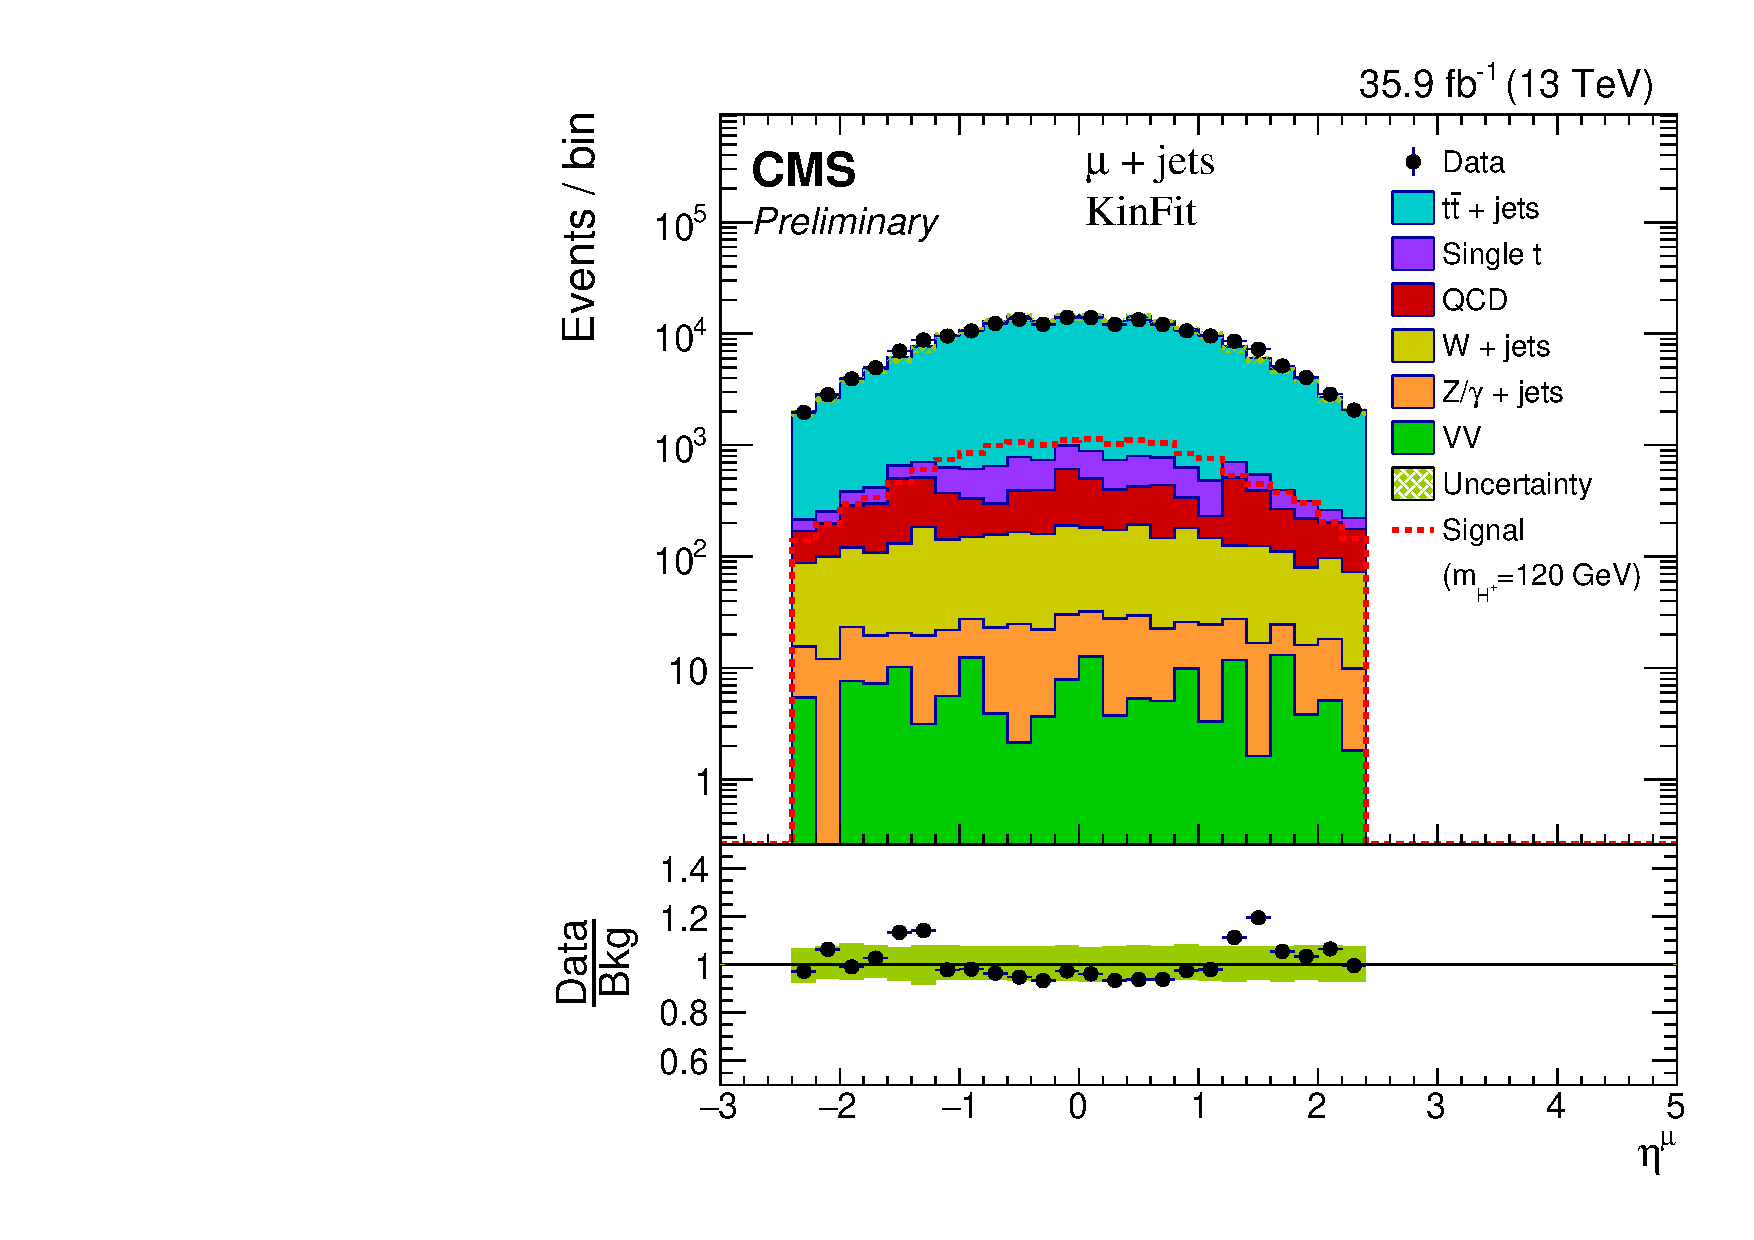
\includegraphics[width=0.40\linewidth]{Image/Muon/KinFit/eta_mu_muKinFit.pdf}}
    \subfigure[$\eta$ of electron]{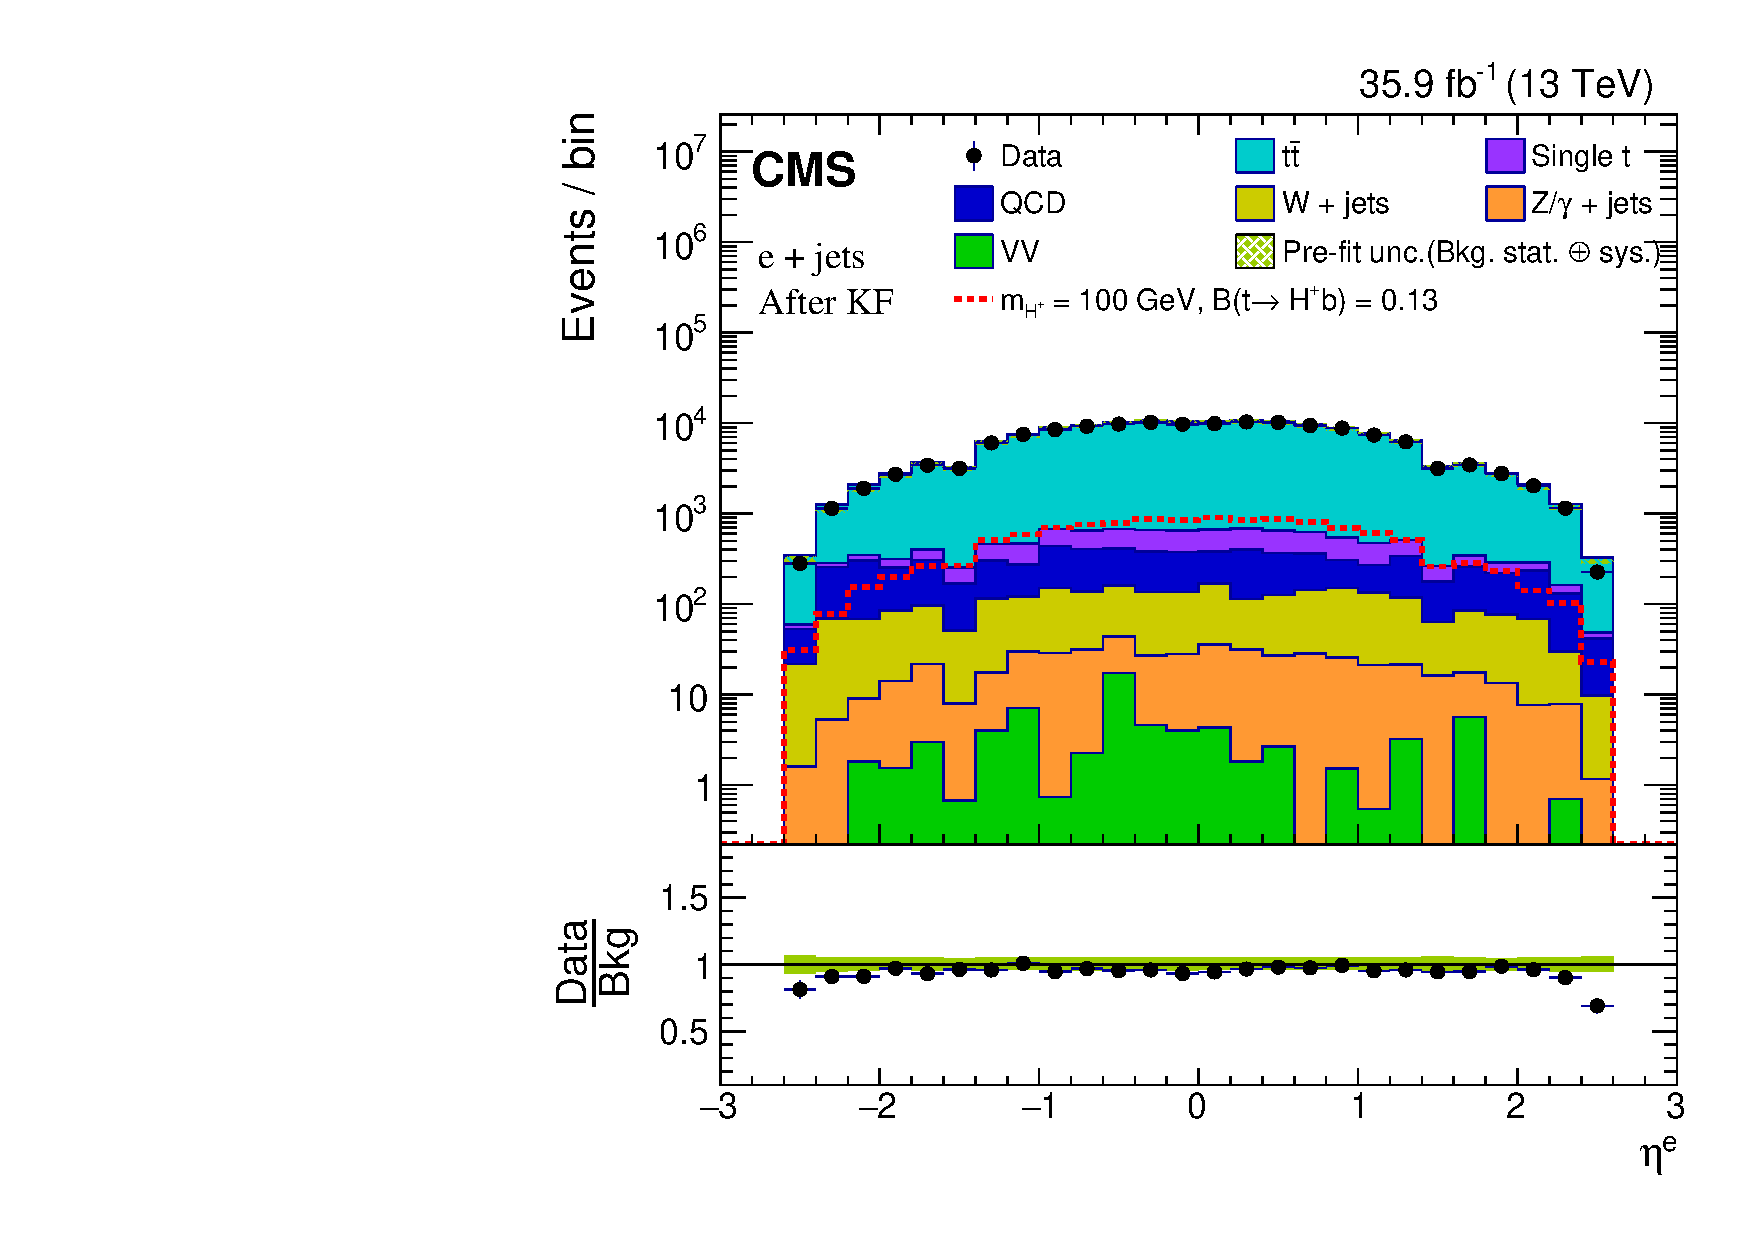
\includegraphics[width=0.40\linewidth]{Image/Electron/KinFit/eta_ele_eleKinFit.pdf}}
    \vfil
    \subfigure[\pt of jets]{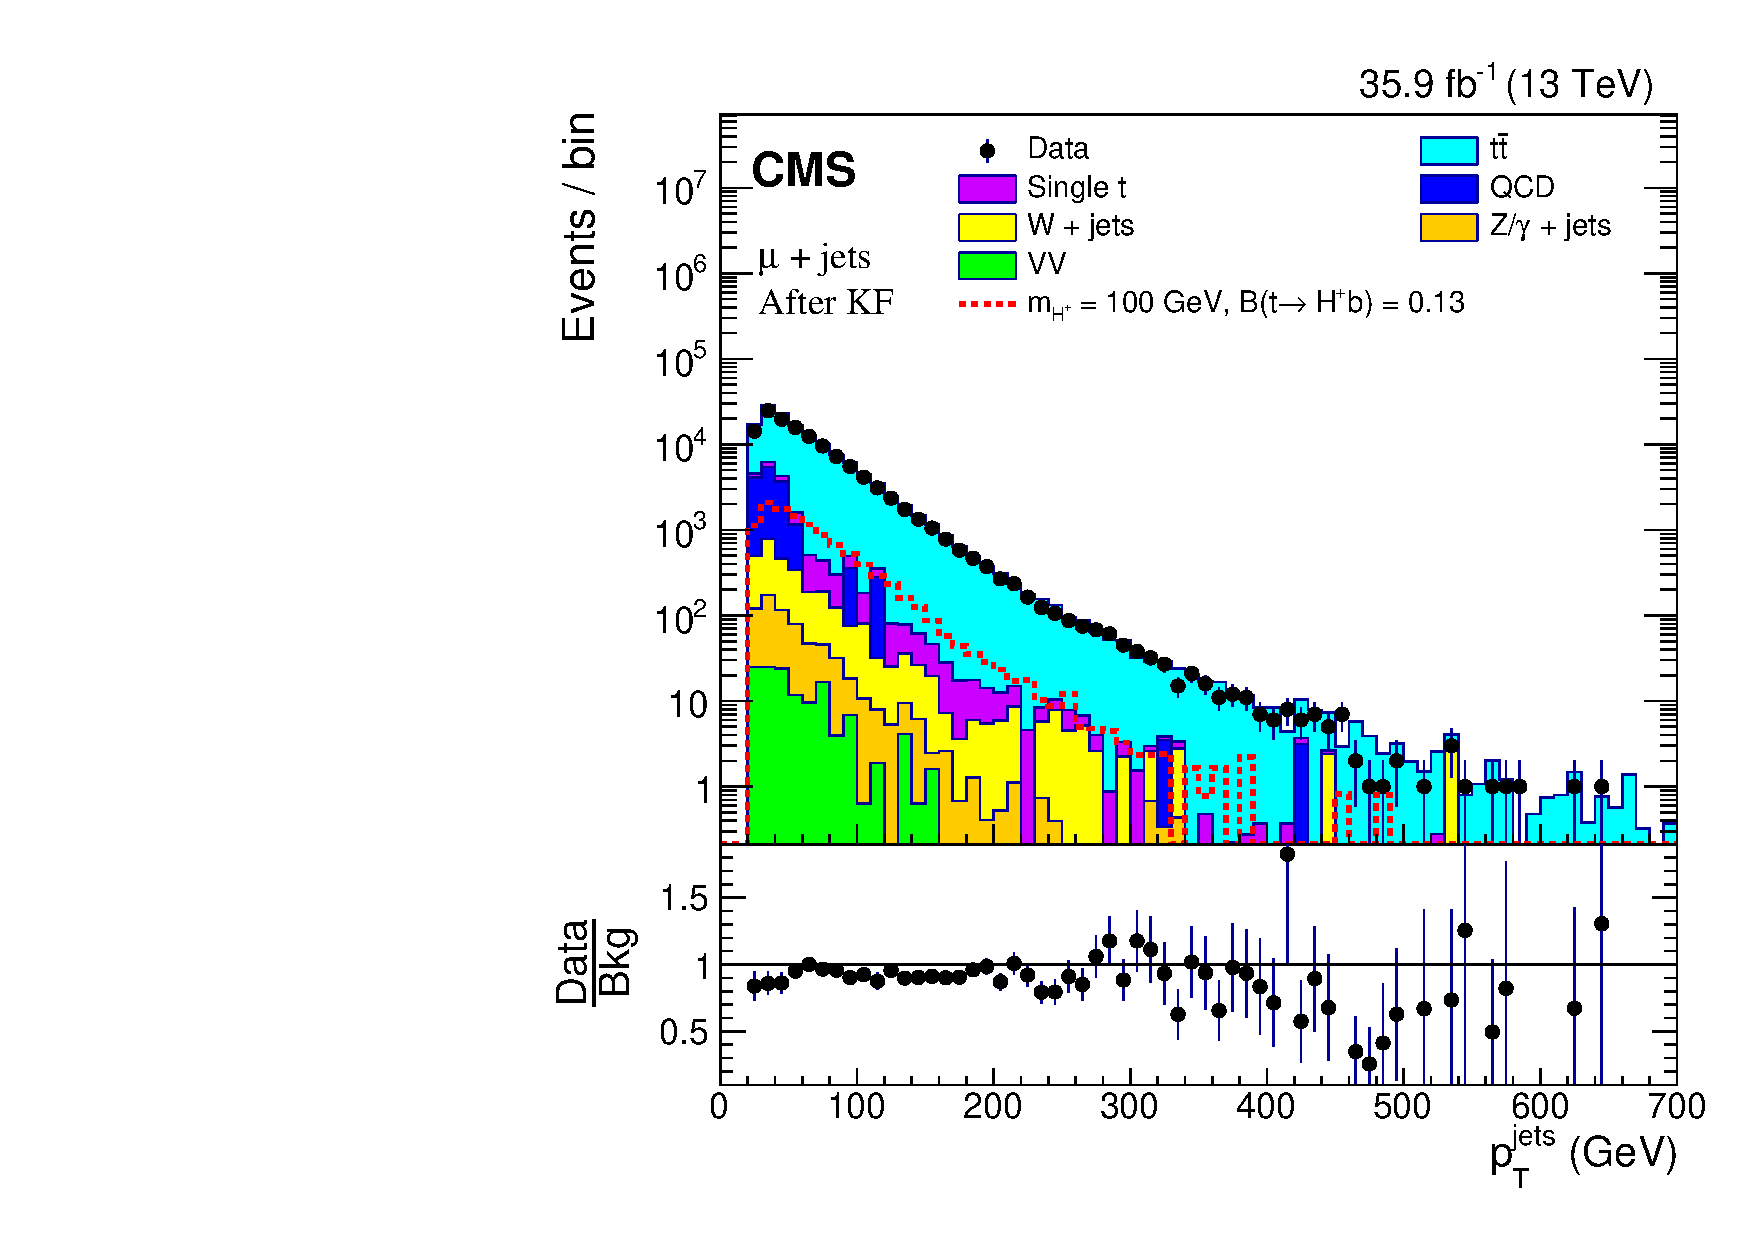
\includegraphics[width=0.40\linewidth]{Image/Muon/KinFit/pt_jet_muKinFit.pdf}}
    \subfigure[\pt of jets]{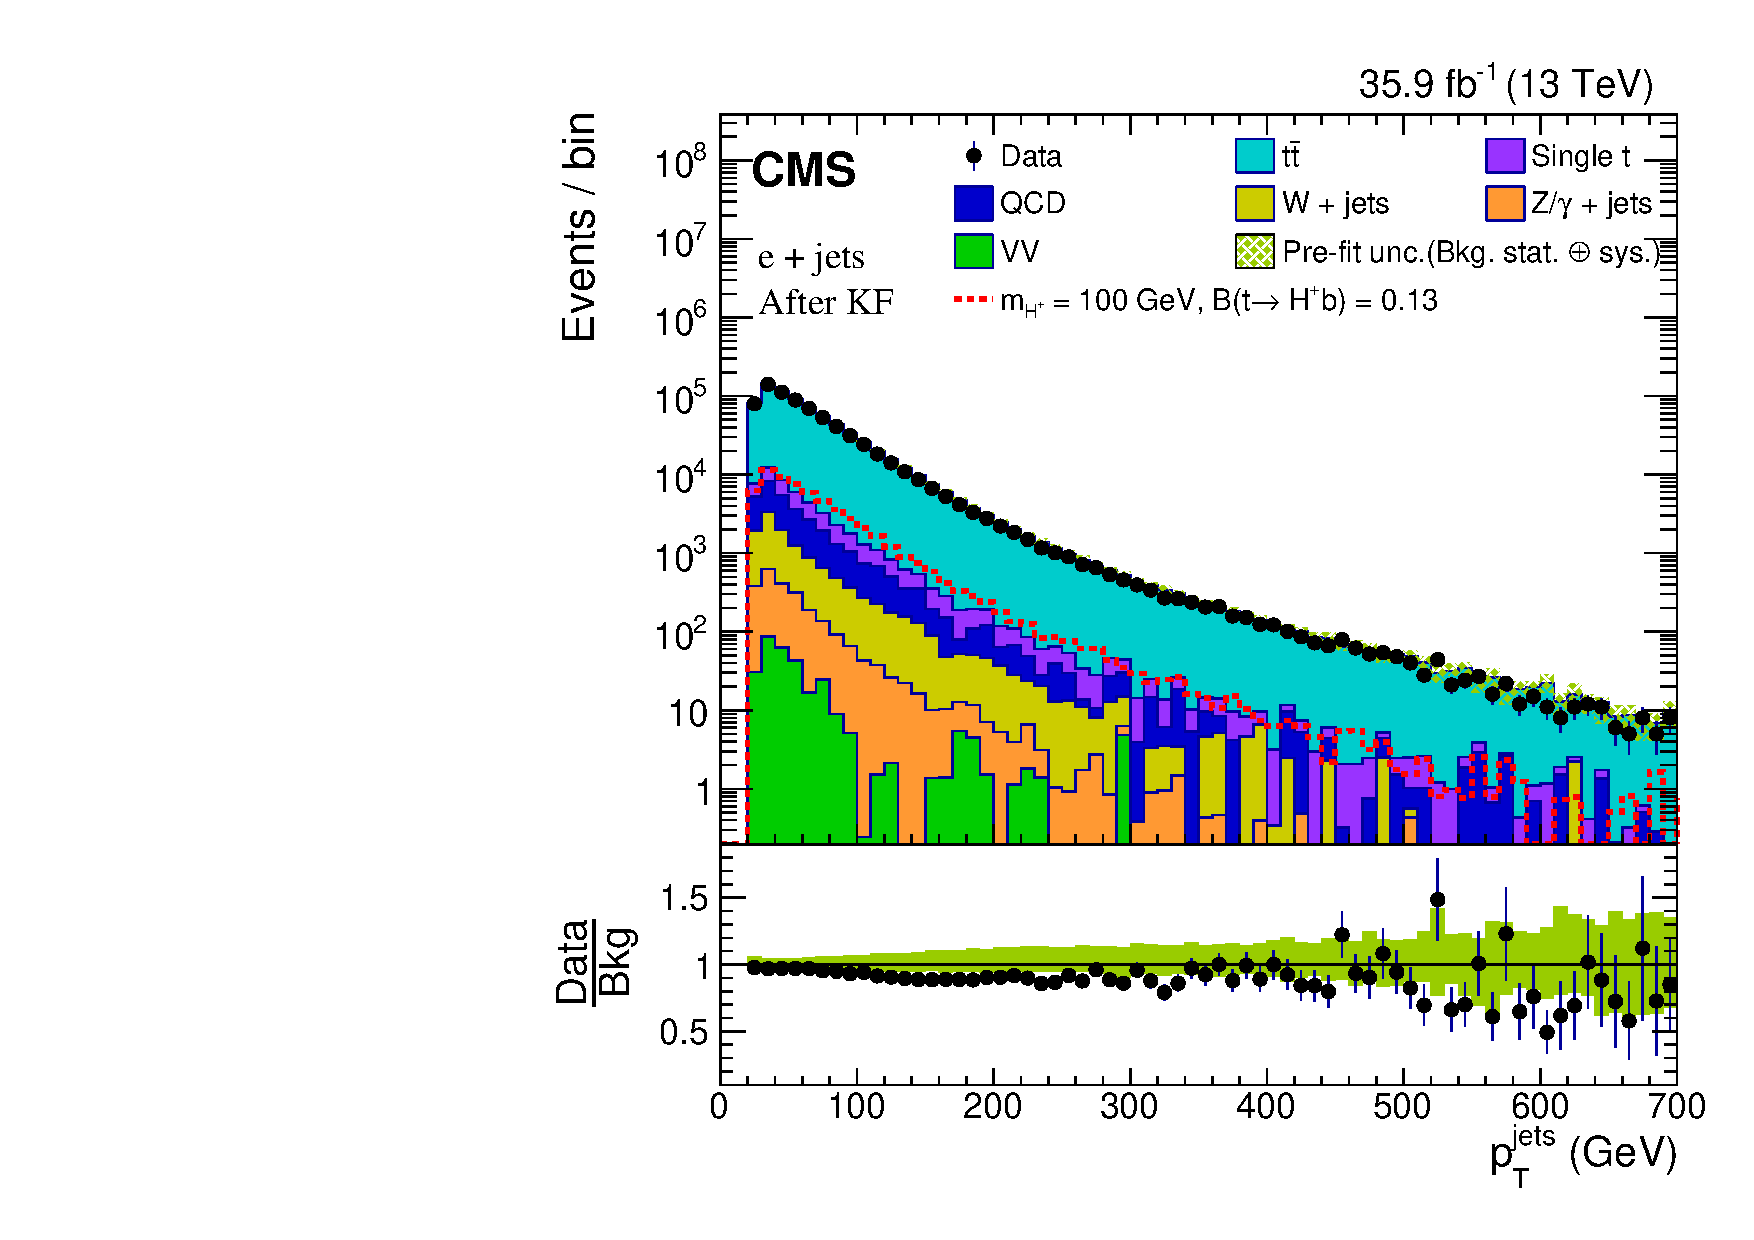
\includegraphics[width=0.40\linewidth]{Image/Electron/KinFit/pt_jet_eleKinFit.pdf}}
    \caption{Distribution of $\pt, \eta$ of kinematic fitted lepton and $\pt$ of jets
    after kinematic fit selection for \mujets and \ejets channel.}
    \label{fig:kfitPlot1}
\end{figure}

%After KinFit:Eta_jets , N_jets, N_bjets
\begin{figure}
    \centering  
    \subfigure[$\eta$ of jets]{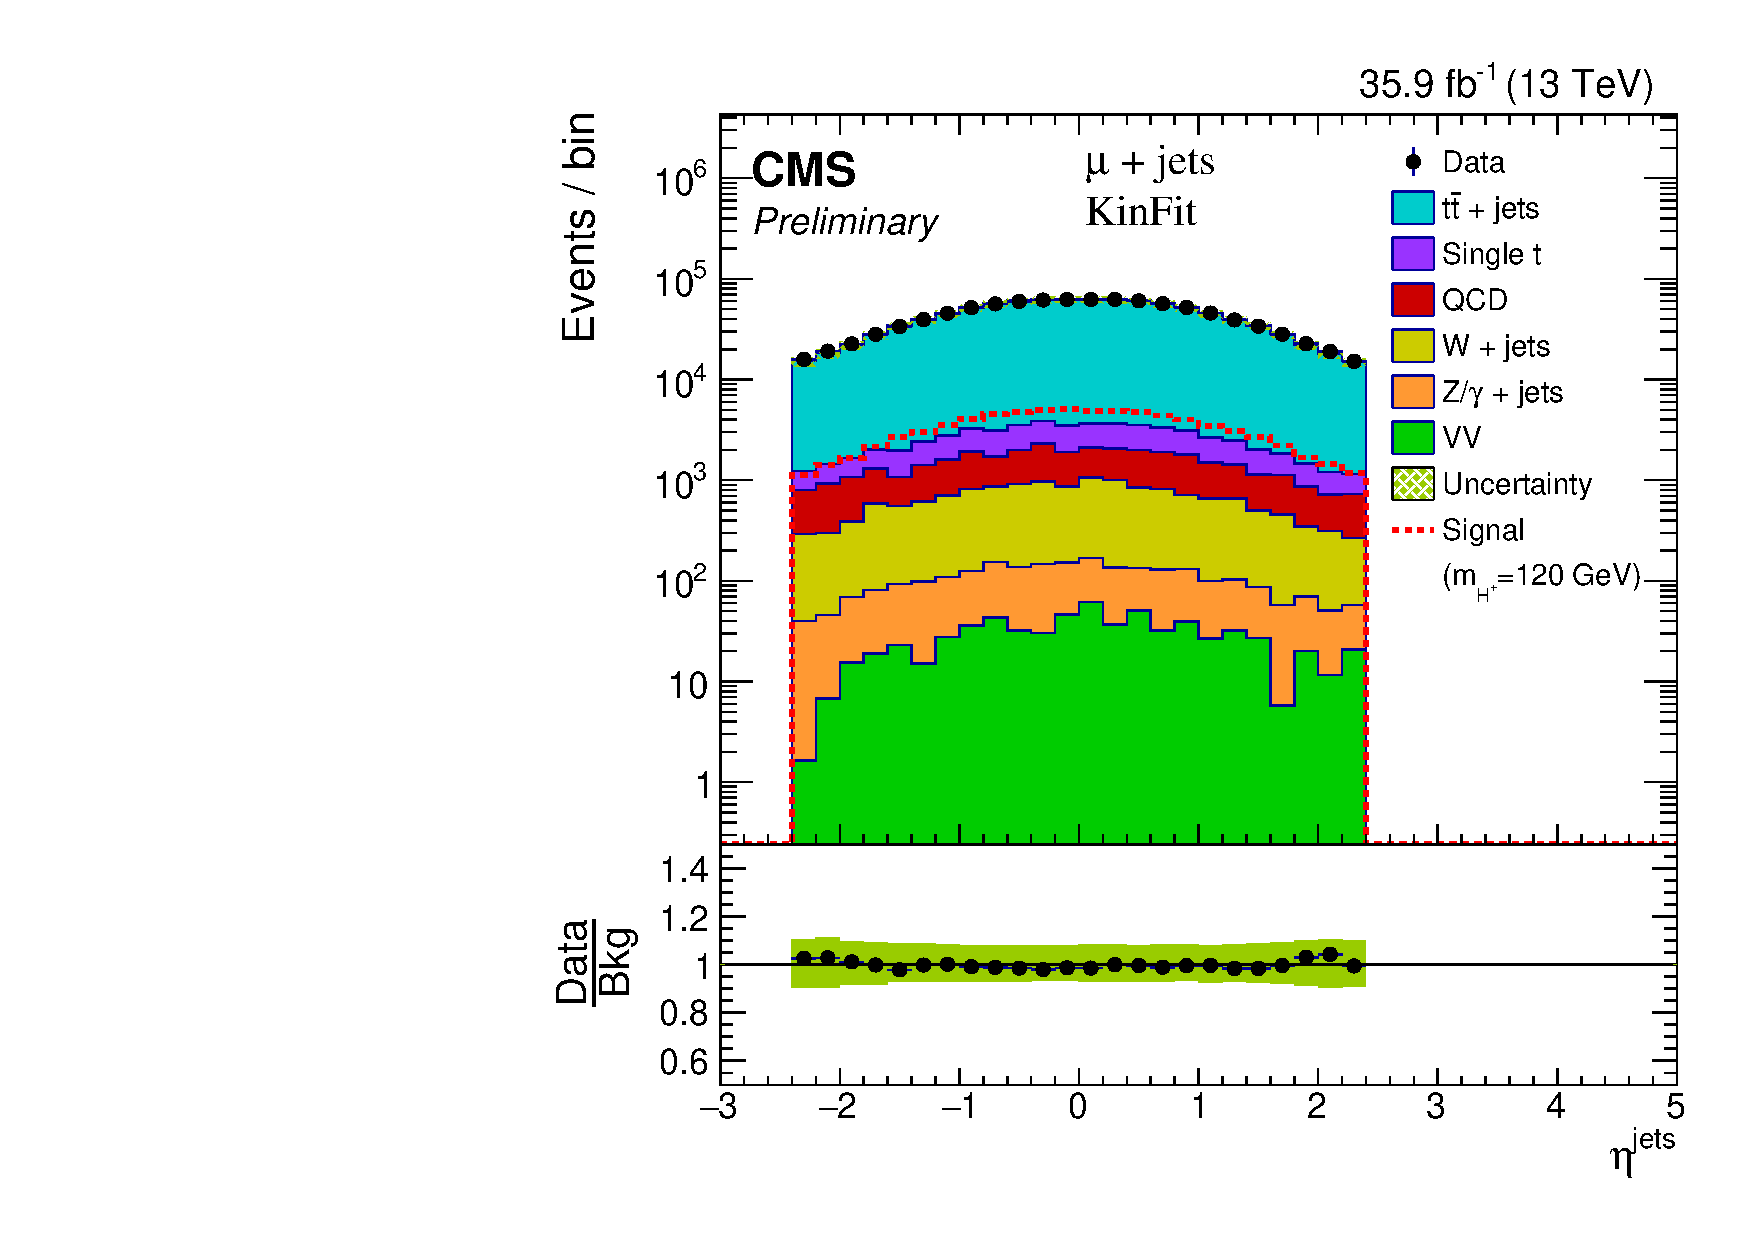
\includegraphics[width=0.40\linewidth]{Image/Muon/KinFit/eta_jet_muKinFit.pdf}}
    \subfigure[$\eta$ of jets]{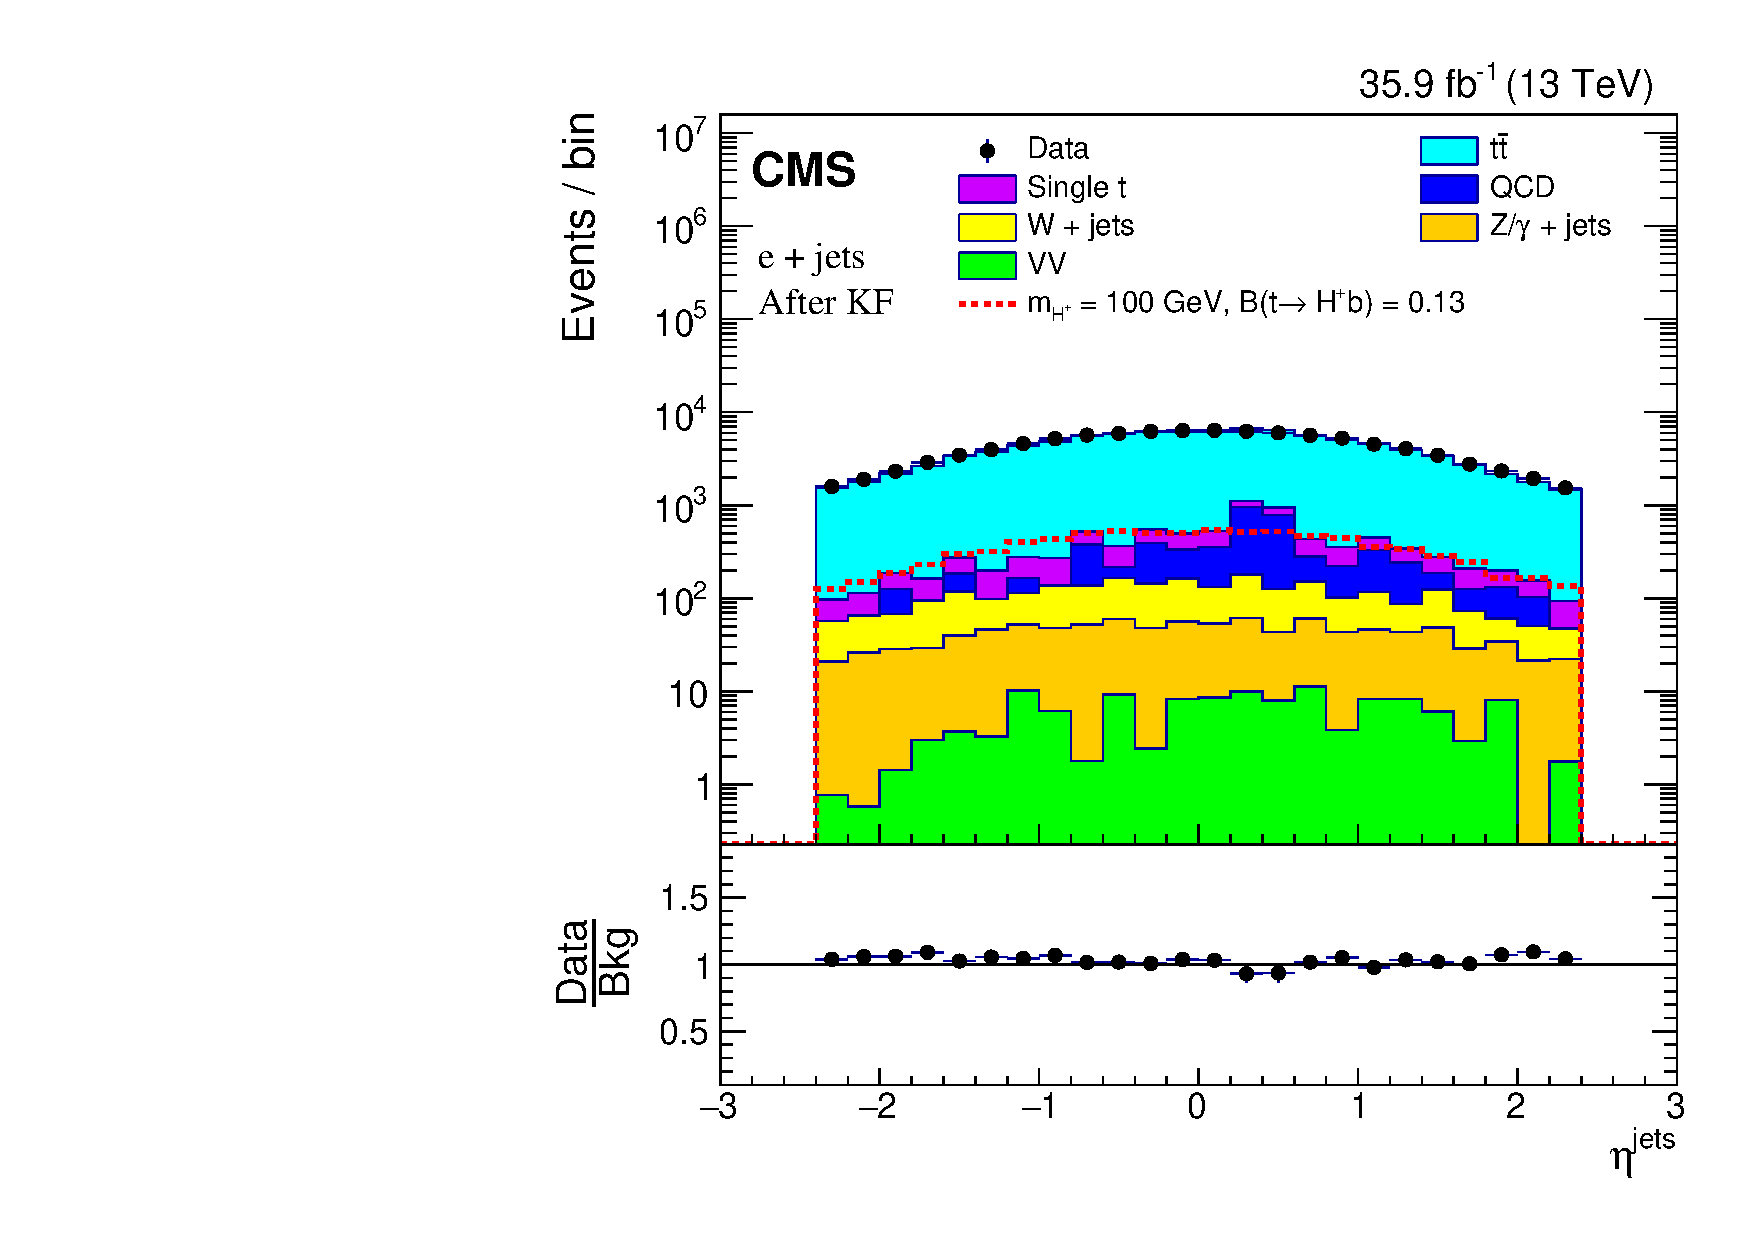
\includegraphics[width=0.40\linewidth]{Image/Electron/KinFit/eta_jet_eleKinFit.pdf}}
    \vfil
    \subfigure[jet multiplicity]{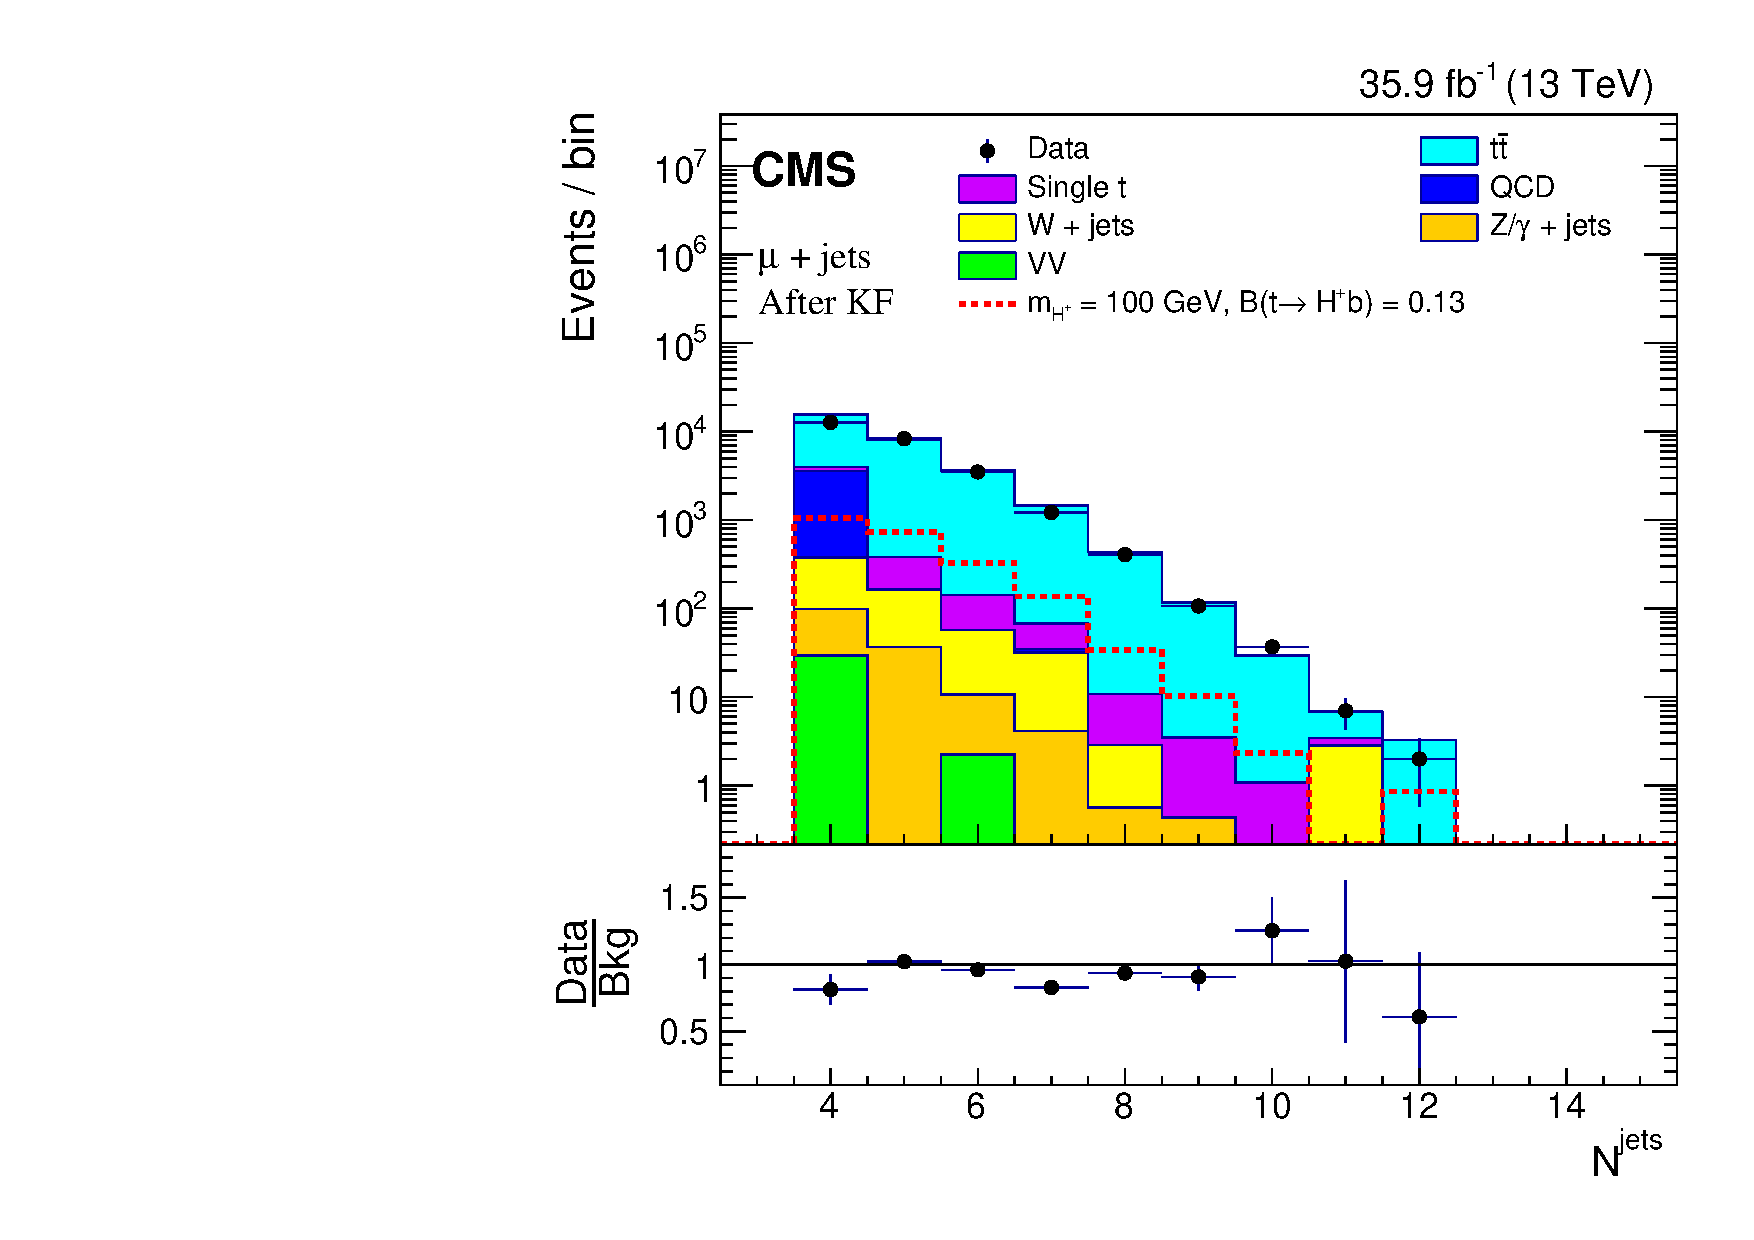
\includegraphics[width=0.40\linewidth]{Image/Muon/KinFit/final_multi_jet_muKinFit.pdf}}
    \subfigure[jet multiplicity]{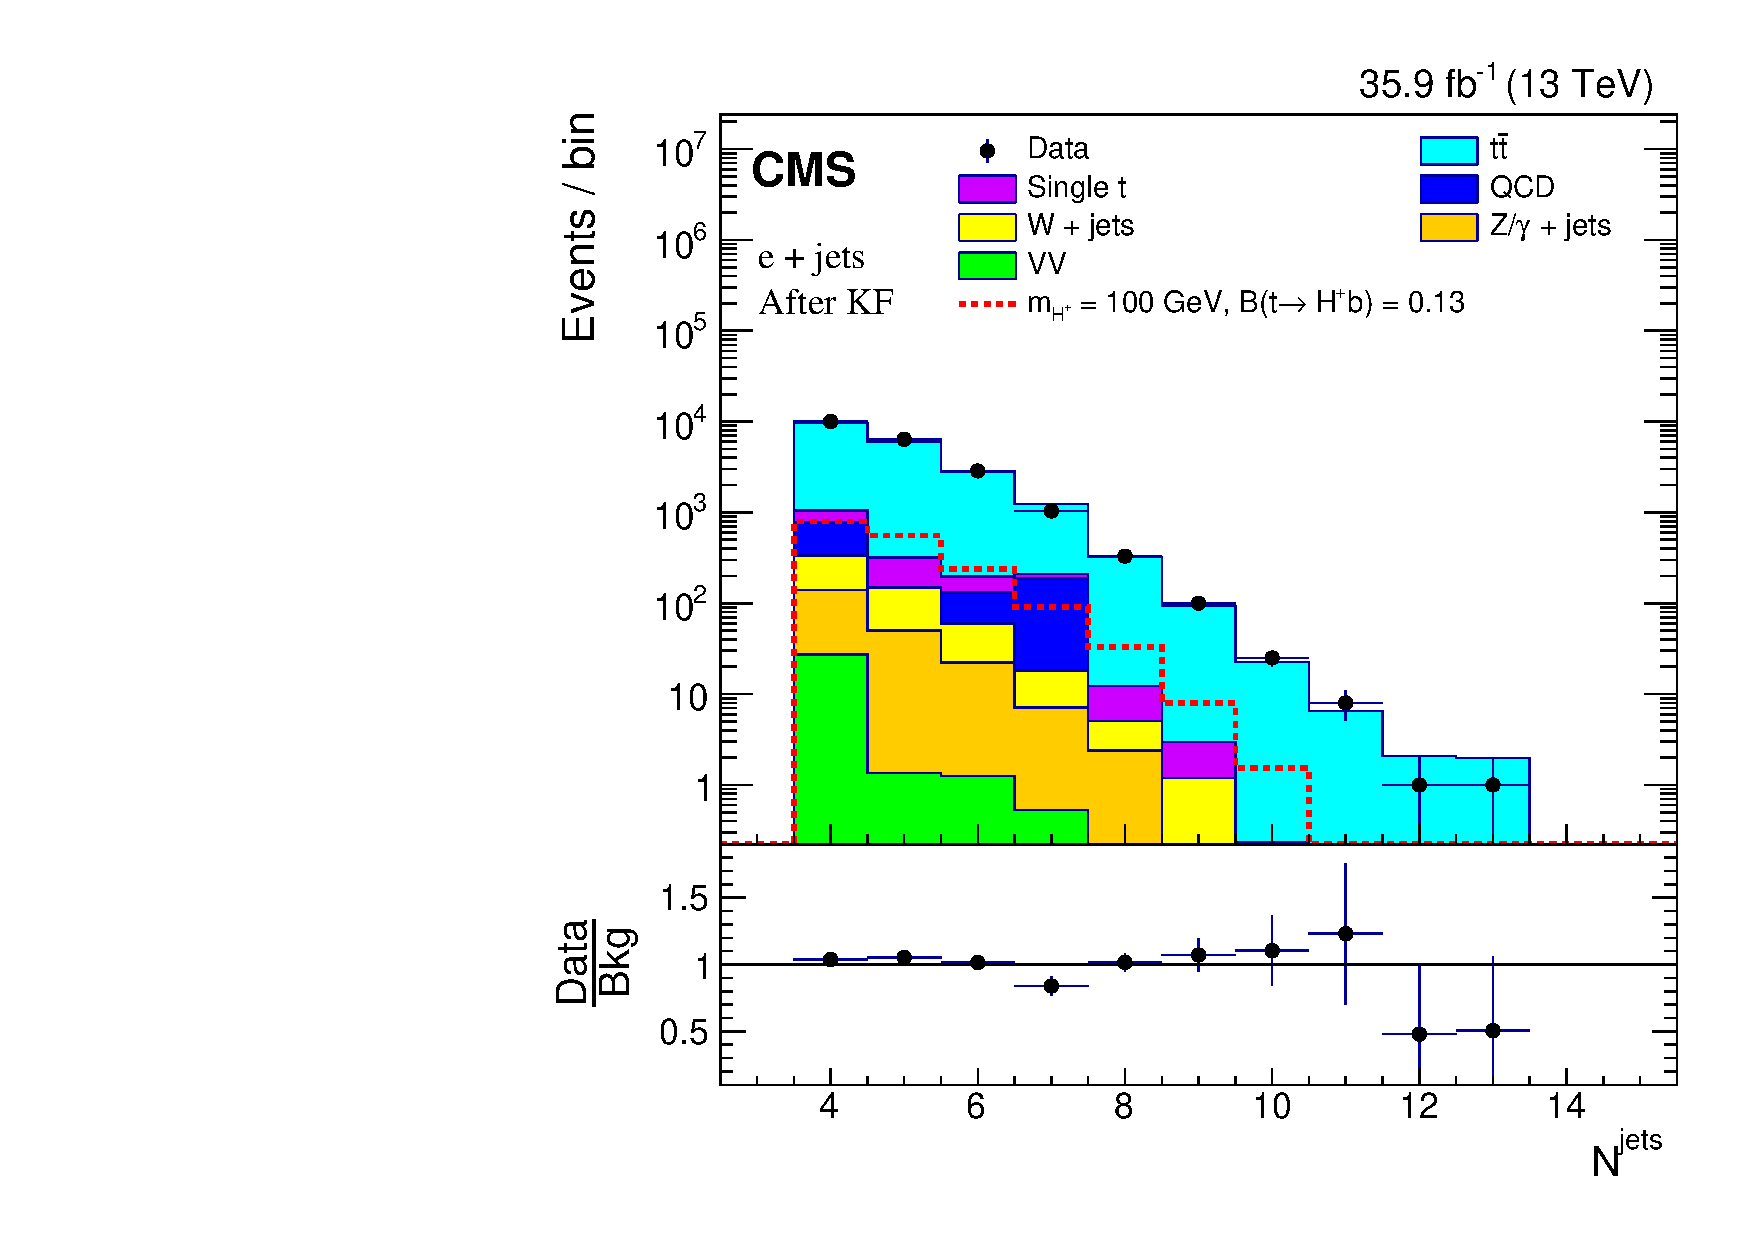
\includegraphics[width=0.40\linewidth]{Image/Electron/KinFit/final_multi_jet_eleKinFit.pdf}}
    \vfil
    \subfigure[\PQb jet multiplicity]{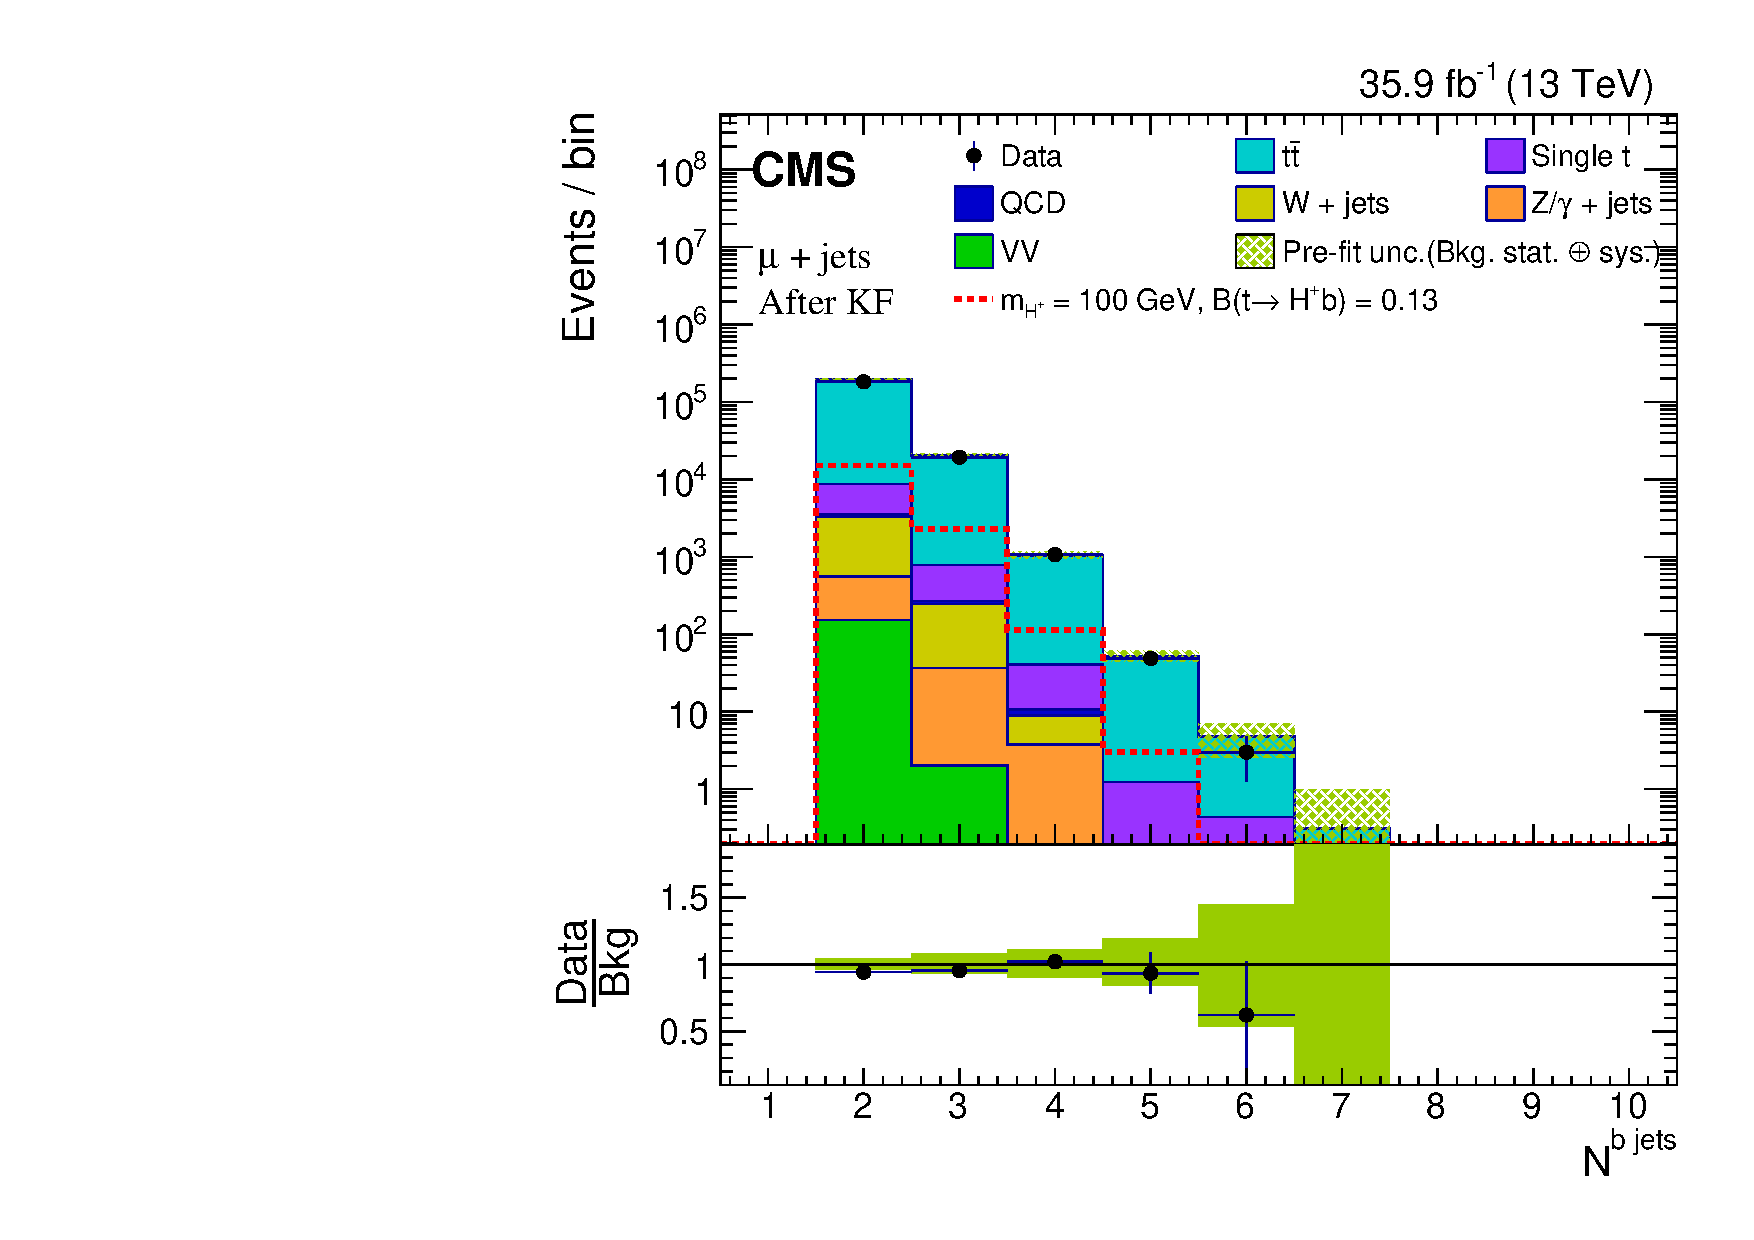
\includegraphics[width=0.40\linewidth]{Image/Muon/KinFit/CSVL_count_muKinFit.pdf}}
    \subfigure[\PQb jet multiplicity]{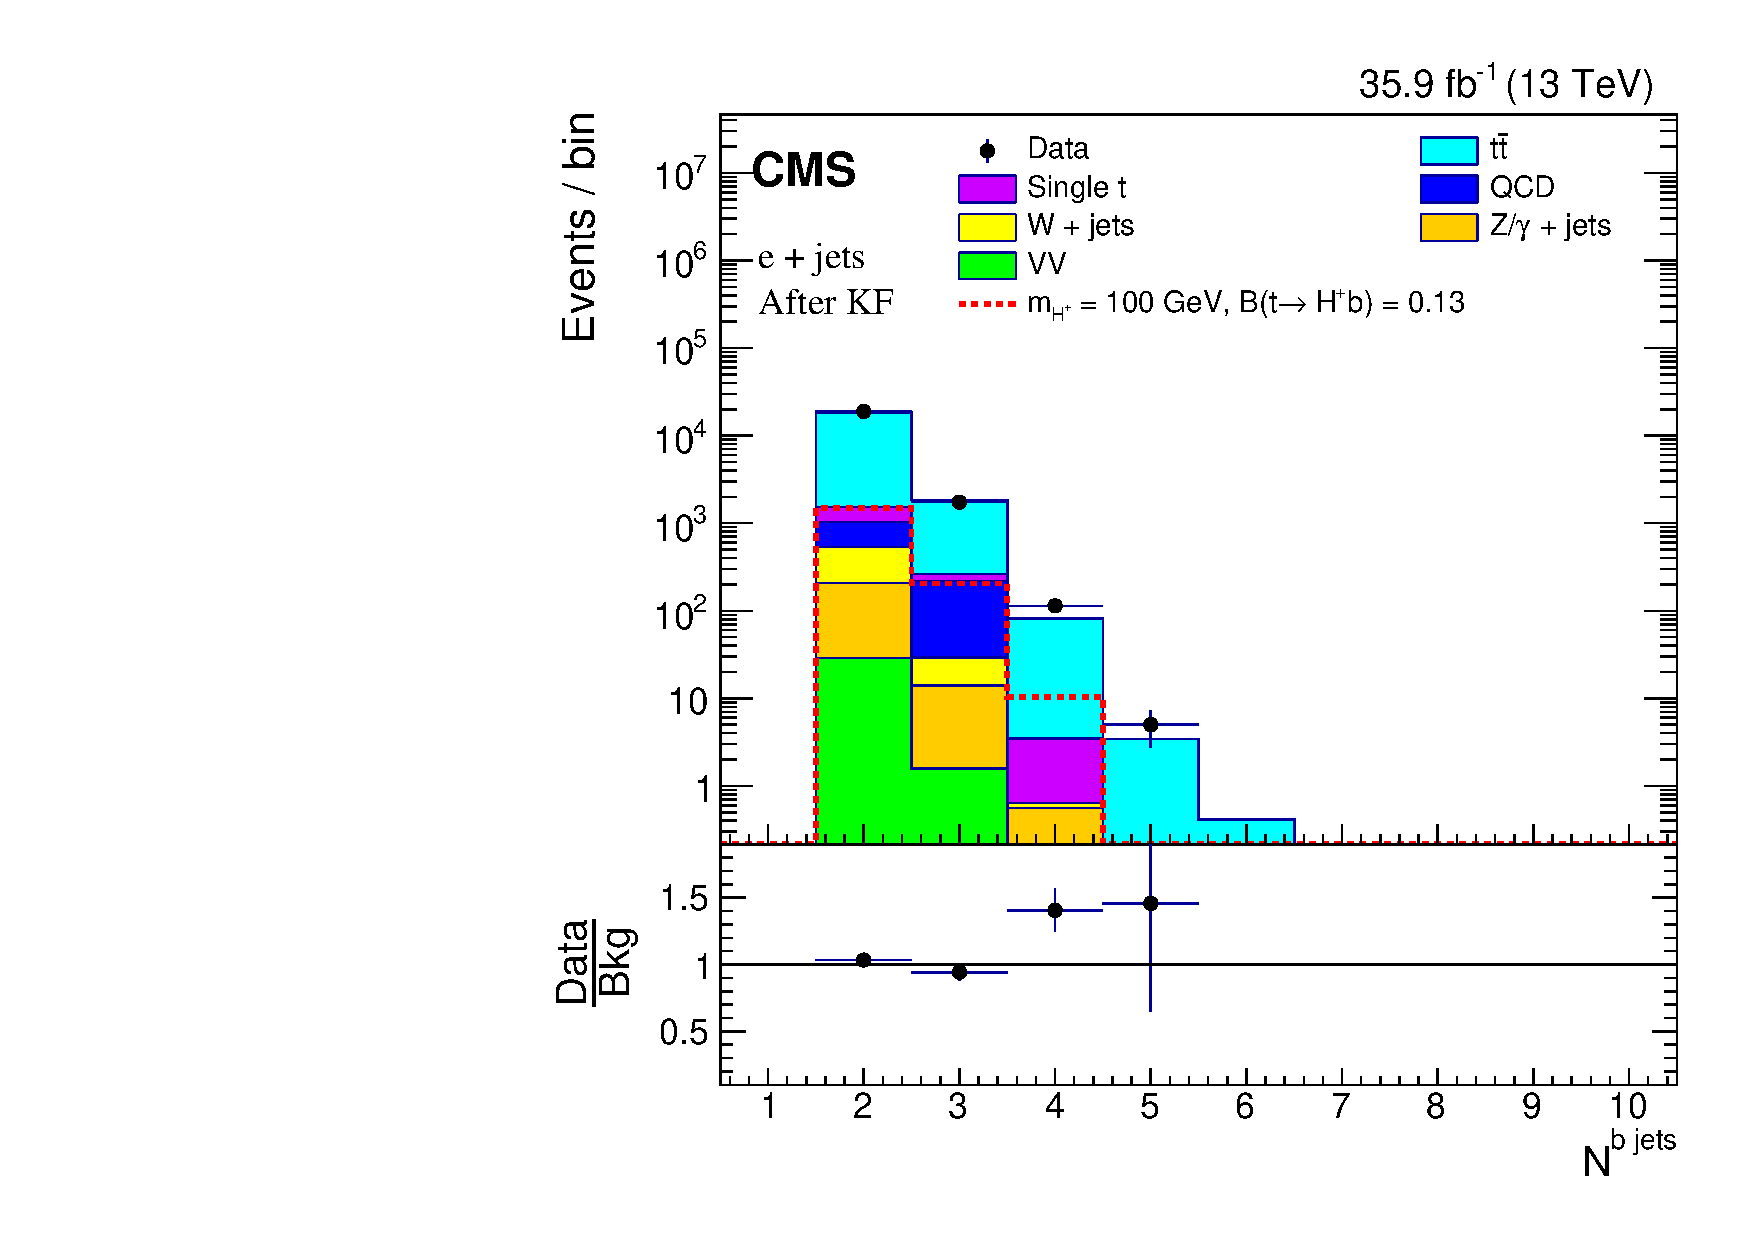
\includegraphics[width=0.40\linewidth]{Image/Electron/KinFit/CSVL_count_eleKinFit.pdf}}
    \caption{Distribution of kinematic fitted $\eta$ of jets, jet multiplicity, and \PQb jet
        multiplicity after kinematic fit selection for \mujets and \ejets channel.}
    \label{fig:kfitPlot2}
\end{figure}

\begin{figure}
    \centering  
    \subfigure[Missing transverse energy]{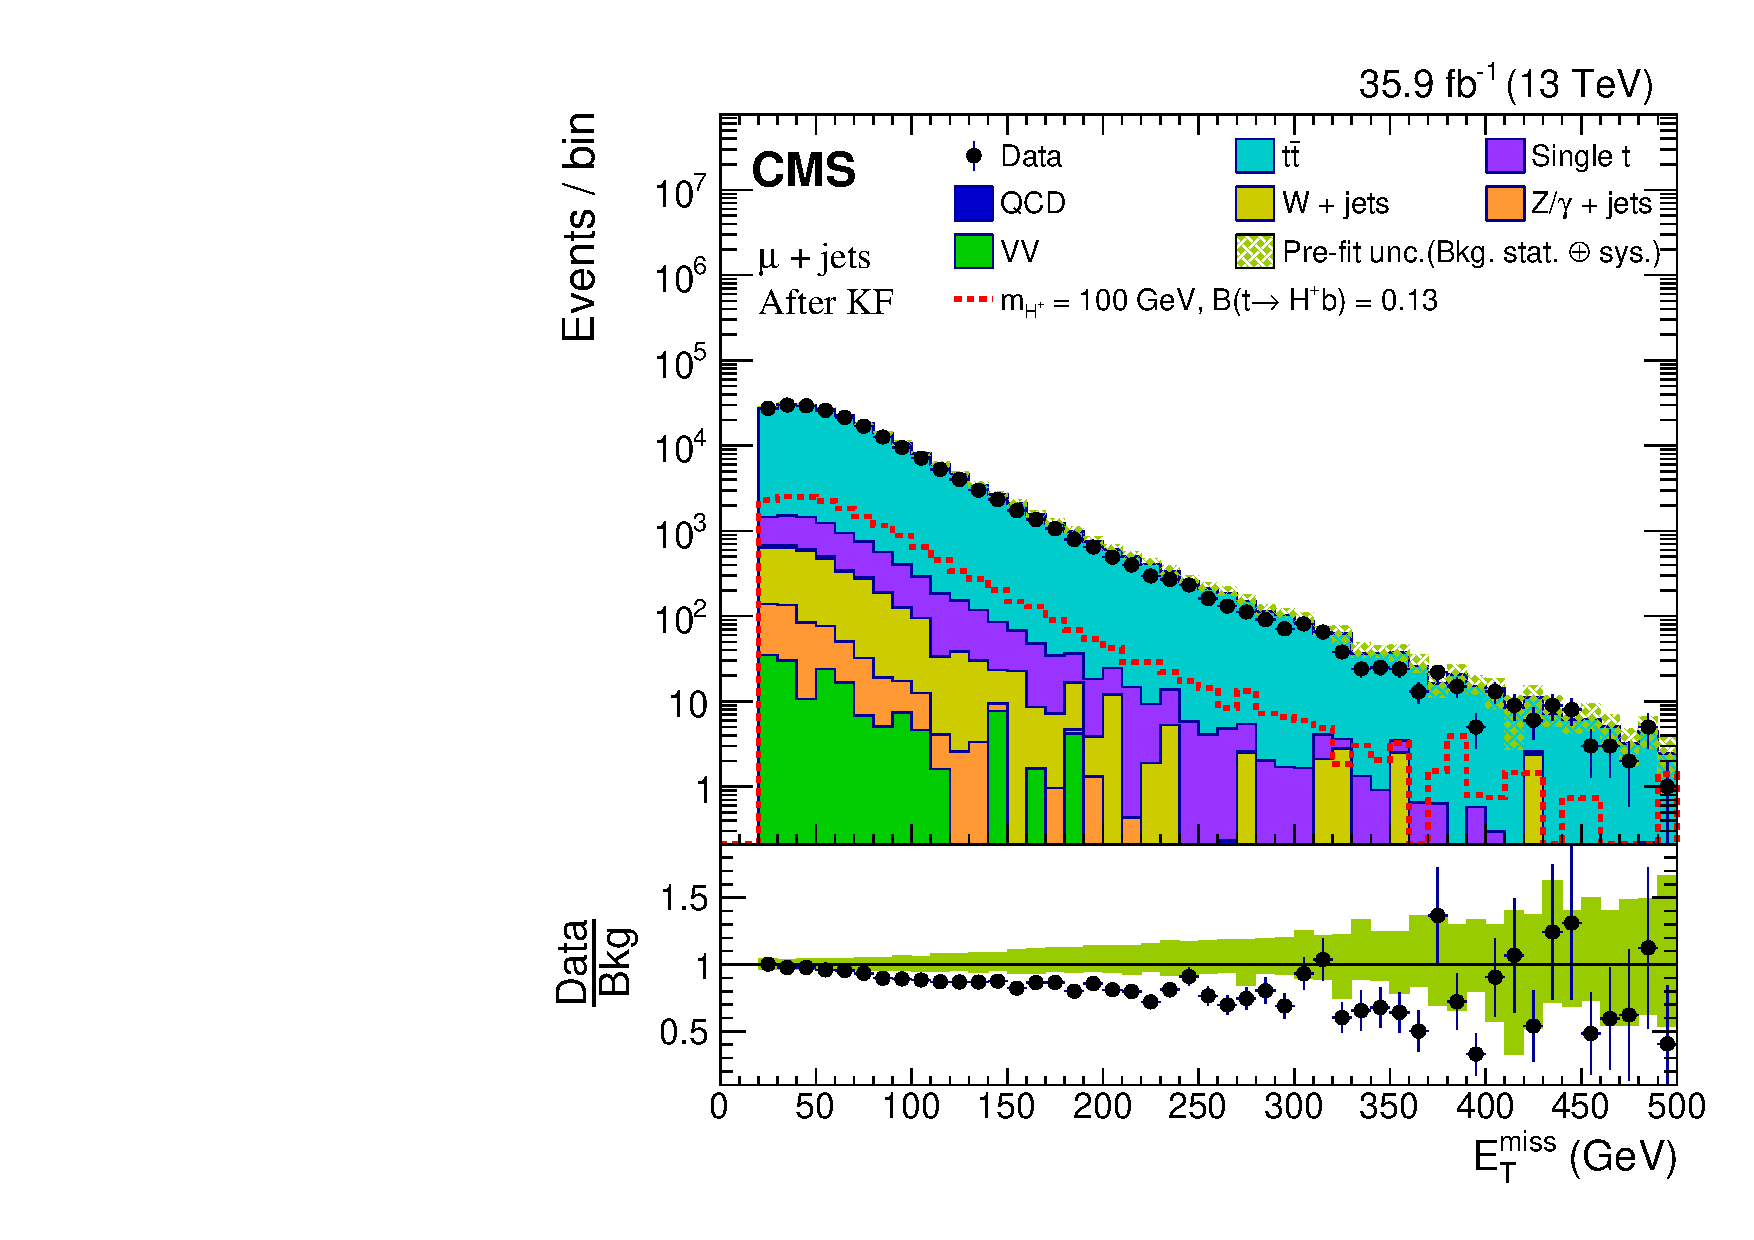
\includegraphics[width=0.45\linewidth]{Image/Muon/KinFit/final_pt_met_muKinFit.pdf}}
    \subfigure[Missing transverse energy]{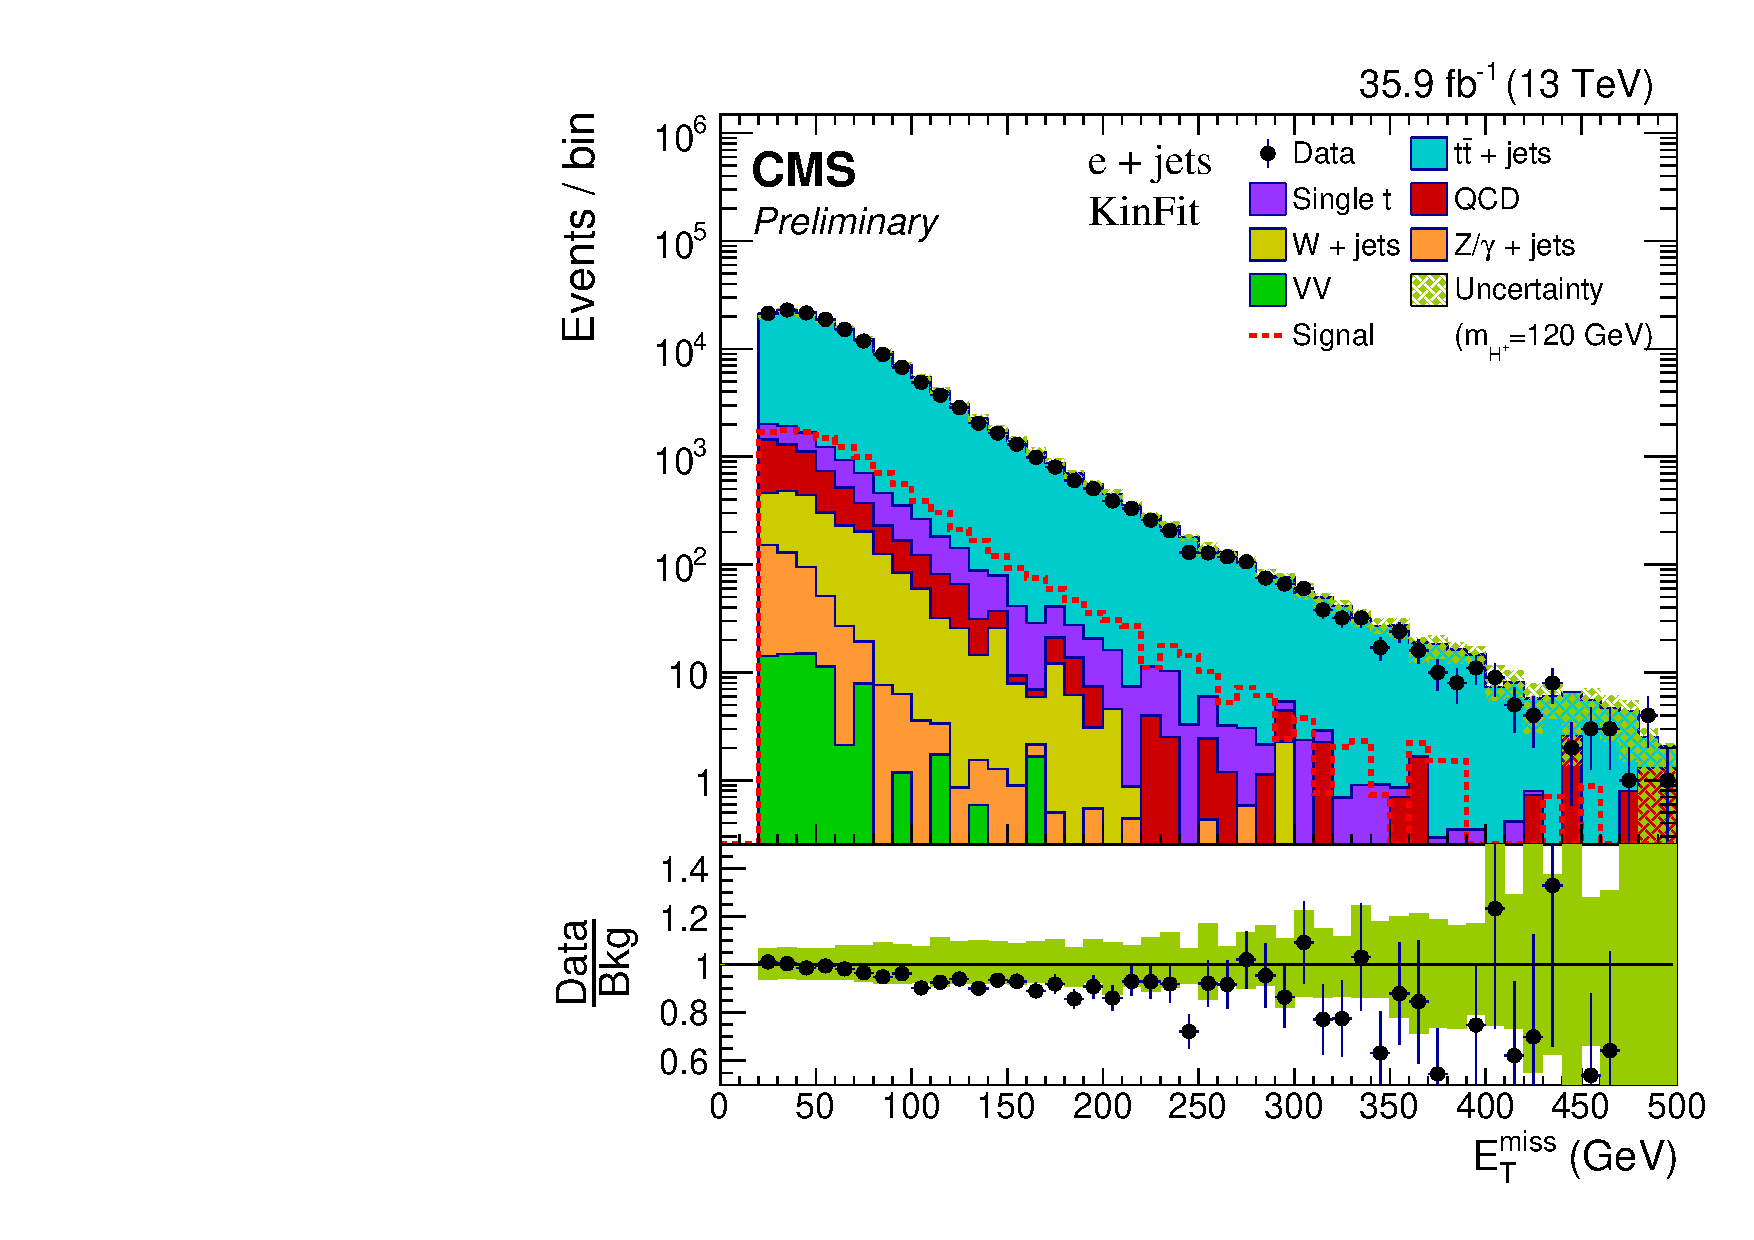
\includegraphics[width=0.45\linewidth]{Image/Electron/KinFit/final_pt_met_eleKinFit.pdf}}
    \vfil
    \subfigure[Transverse mass of \PW boson]{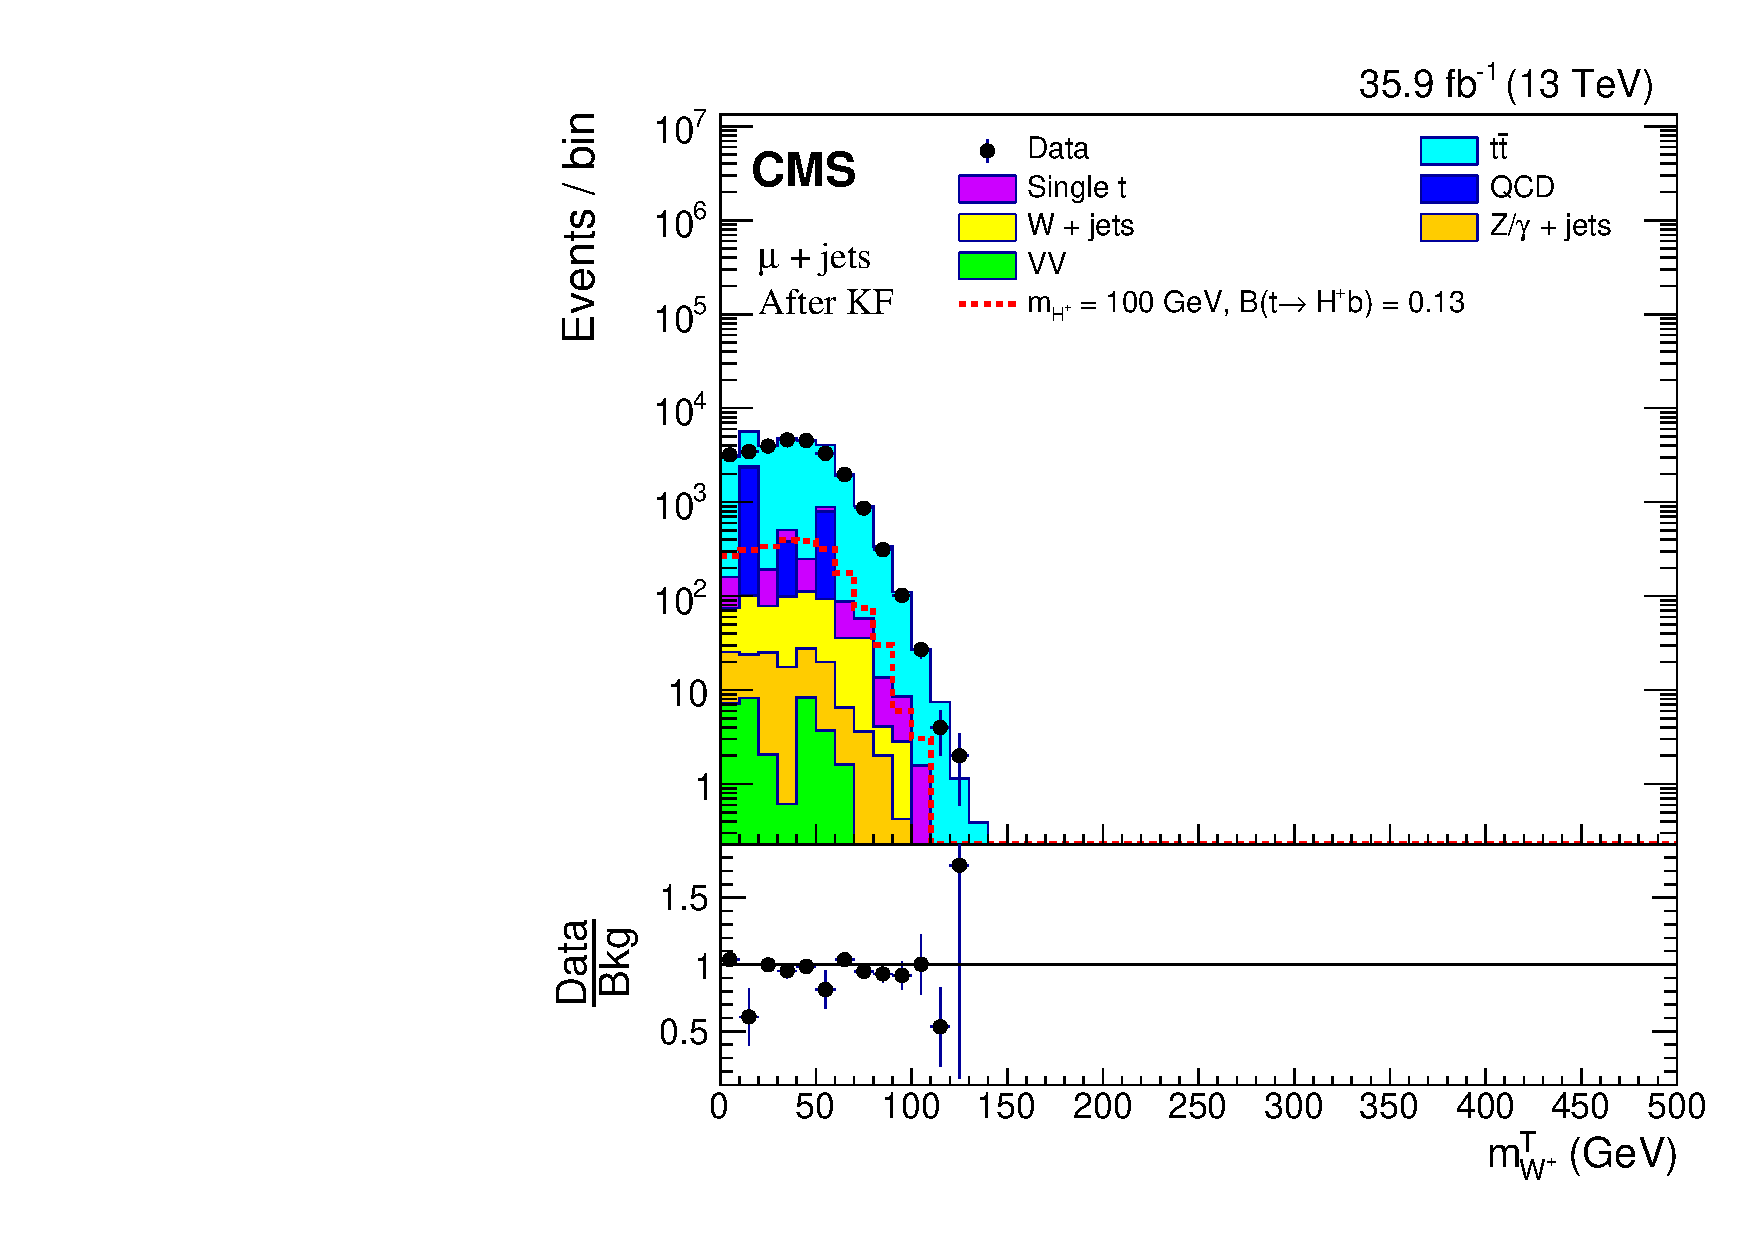
\includegraphics[width=0.45\linewidth]{Image/Muon/KinFit/wmt_muKinFit.pdf}}
    \subfigure[Transverse mass of \PW boson]{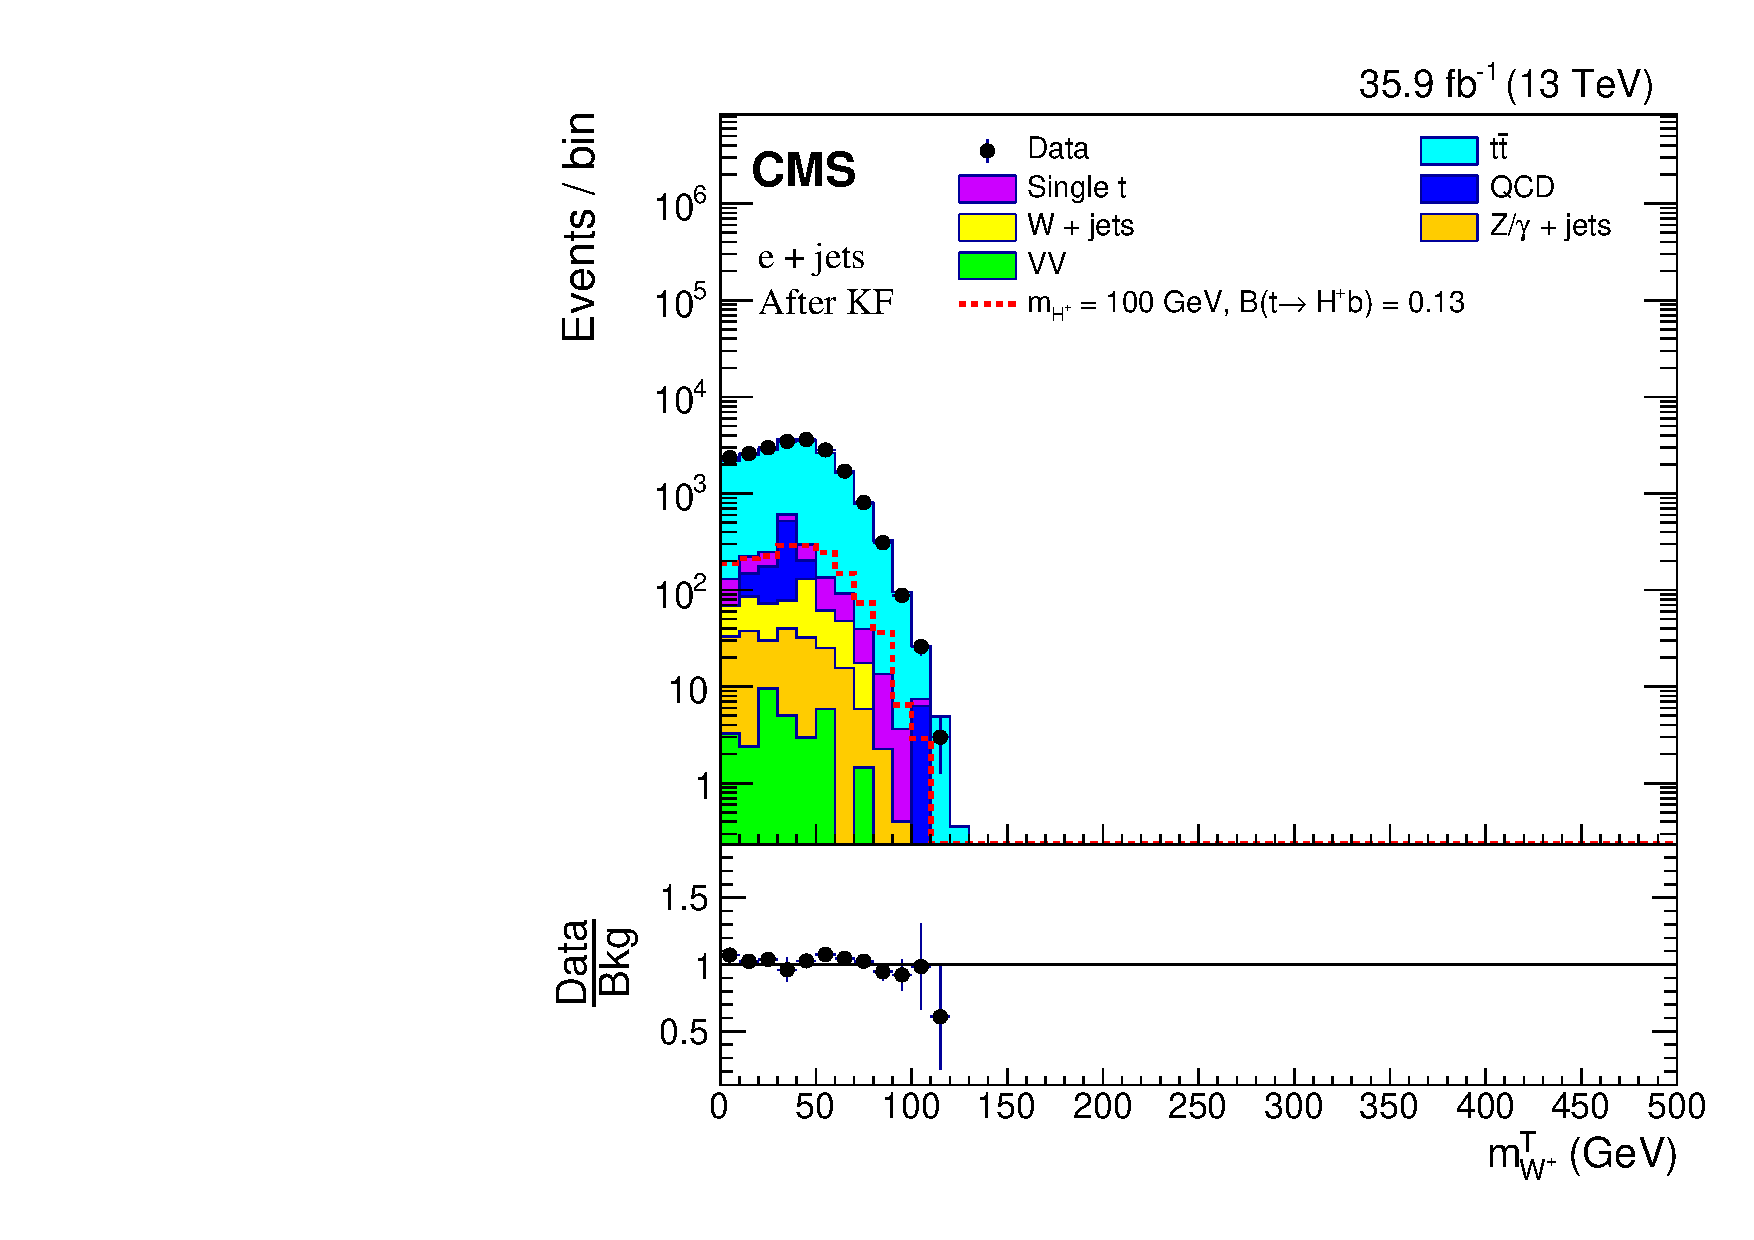
\includegraphics[width=0.45\linewidth]{Image/Electron/KinFit/wmt_eleKinFit.pdf}}
    \caption{Distribution of kinematic fitted $\MET$ and $m_{\PW^+}^{T}$ after kinematic fit selection 
	for \mujets and \ejets channel.}
    \label{fig:kfitPlot3}
\end{figure}



%-------------------------------------
% c-tagging
%-------------------------------------
\section{c-jet Tagging}
\label{s:cTag}

As the charged Higgs Boson decays to a charm and an anti-strange quark, the
identification of charm jet is expected to increase the signal significance.
The charm tagging or c-tagging is recently developed in the CMS collaboration
~\cite{CMS-PAS-BTV-16-001} based on the CSV method for the analyses at 13 TeV 
data. This procedure is similar to that of b-tagging described in 
Section~\ref{s:bTag}. At the end, we have two charm discriminators: charm 
vs. b-jet (pfCCvsB) and charm vs. light jet (pfCCvsL). Distribution of these 
two discriminators is shown in Figure~\ref{fig:pfCCvsBL} for the \mujets and
\ejets channel. These are collectively used to tag a jet as a c-jet.
Three working points are provided by BTV POG for the charm tagging, as shown 
in Table (\ref{tab:cTagEff}) and Figure~\ref{fig:cTagger}.

At least one of the light jets from hadronic decay mode of \ttbar is required 
to pass one of the charm-jet working points. First, each WP was separately used
for c-tagging. However, the limits were not getting improved for medium and tight 
working points. Therefore the loose WP is finally used. Although the signal to
background ratio increases as one goes from loose to tight working point, 
the limits are not improved because the event yield also goes down. However,
it is found that, as described in Section (\ref{ss:mjj_cTagEx}), that if the 
events after KinFit selection are exclusively divided into the categories 
based on loose, medium, and the tight charm working points and the limit is 
computed by combining data cards from these three categories, as described in 
Section (\ref{ss:limit_cTagEx}), then the limit is improved.
\begin{table}
\caption{The efficiency of loose, medium, and tight c-tag working points for
    different quark-flavor of jets \cite{Sirunyan:2017ezt}. These efficiencies 
    are calculated from
\ttbar events with jet \pt $>$ 20 GeV.}
\label{tab:cTagEff}
\begin{center}
\begin{tabular}{cccccc}
\hline
\hline
WP & $\epsilon^c$ (\%) & $\epsilon^b$ (\%) & $\epsilon^{udsg}$ (\%) & pfCCvsL & pfCBvsB\\ \hline\hline
c-tagger L & 88 & 36 & 91 & $>$ -0.48 & $>$ -0.17 \\
c-tagger M & 40 & 17 & 19 & $>$ -0.1  & $>$  0.08 \\
c-tagger T & 19 & 20 & 1.2& $>$ 0.69  & $>$ -0.45 \\
\hline
\end{tabular}
\end{center}
\end{table}
%ctag eff figure
\begin{figure}
\centering
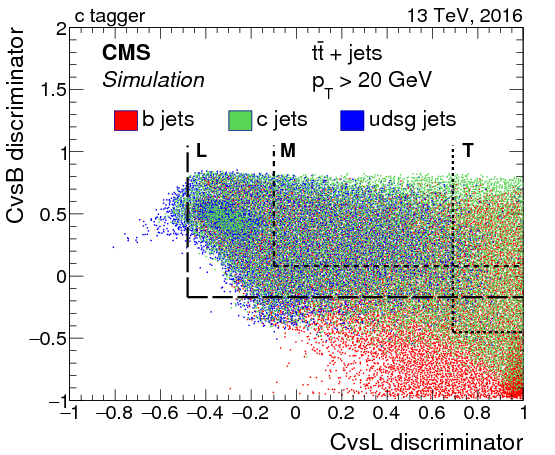
\includegraphics[width=0.6\linewidth]{Image/cTagger.png}
\caption{The 2D plot between charm-taggers. The region right to the vertical 
    and above to the horizontal line correspond to different charm working 
    points (WPs). Unlike the b-tag WPs, there is an overlap between the loose,
    medium, and tight c-tag WPs. This figure is taken from
~\cite{CMS-PAS-BTV-16-001}.}
\label{fig:cTagger}
\end{figure}

\begin{figure}
\centering
\subfigure[charm vs. b-jet discriminator ]{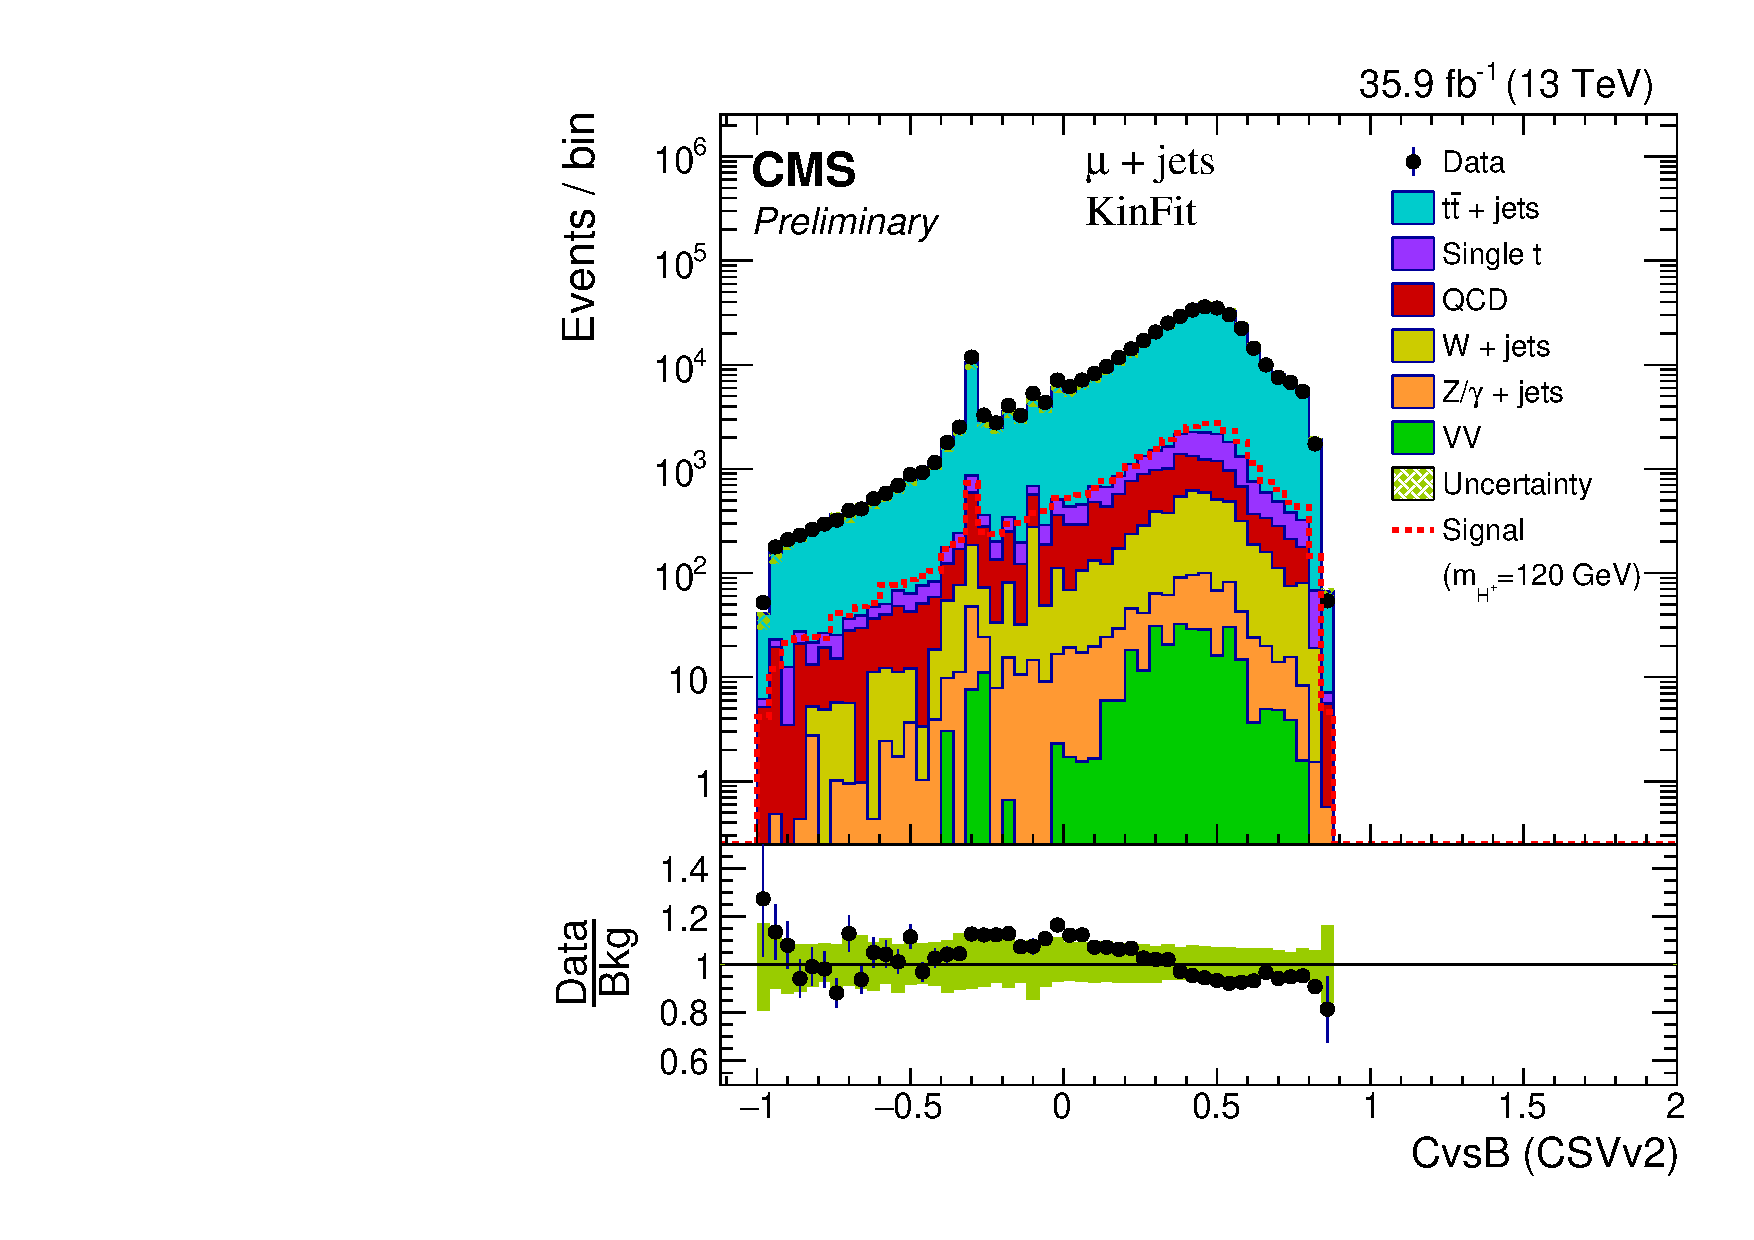
\includegraphics[width=0.50\linewidth]{Image/Muon/KinFit/pfCCvsB_muKinFit.pdf}}
\subfigure[charm vs. b-jet discriminator ]{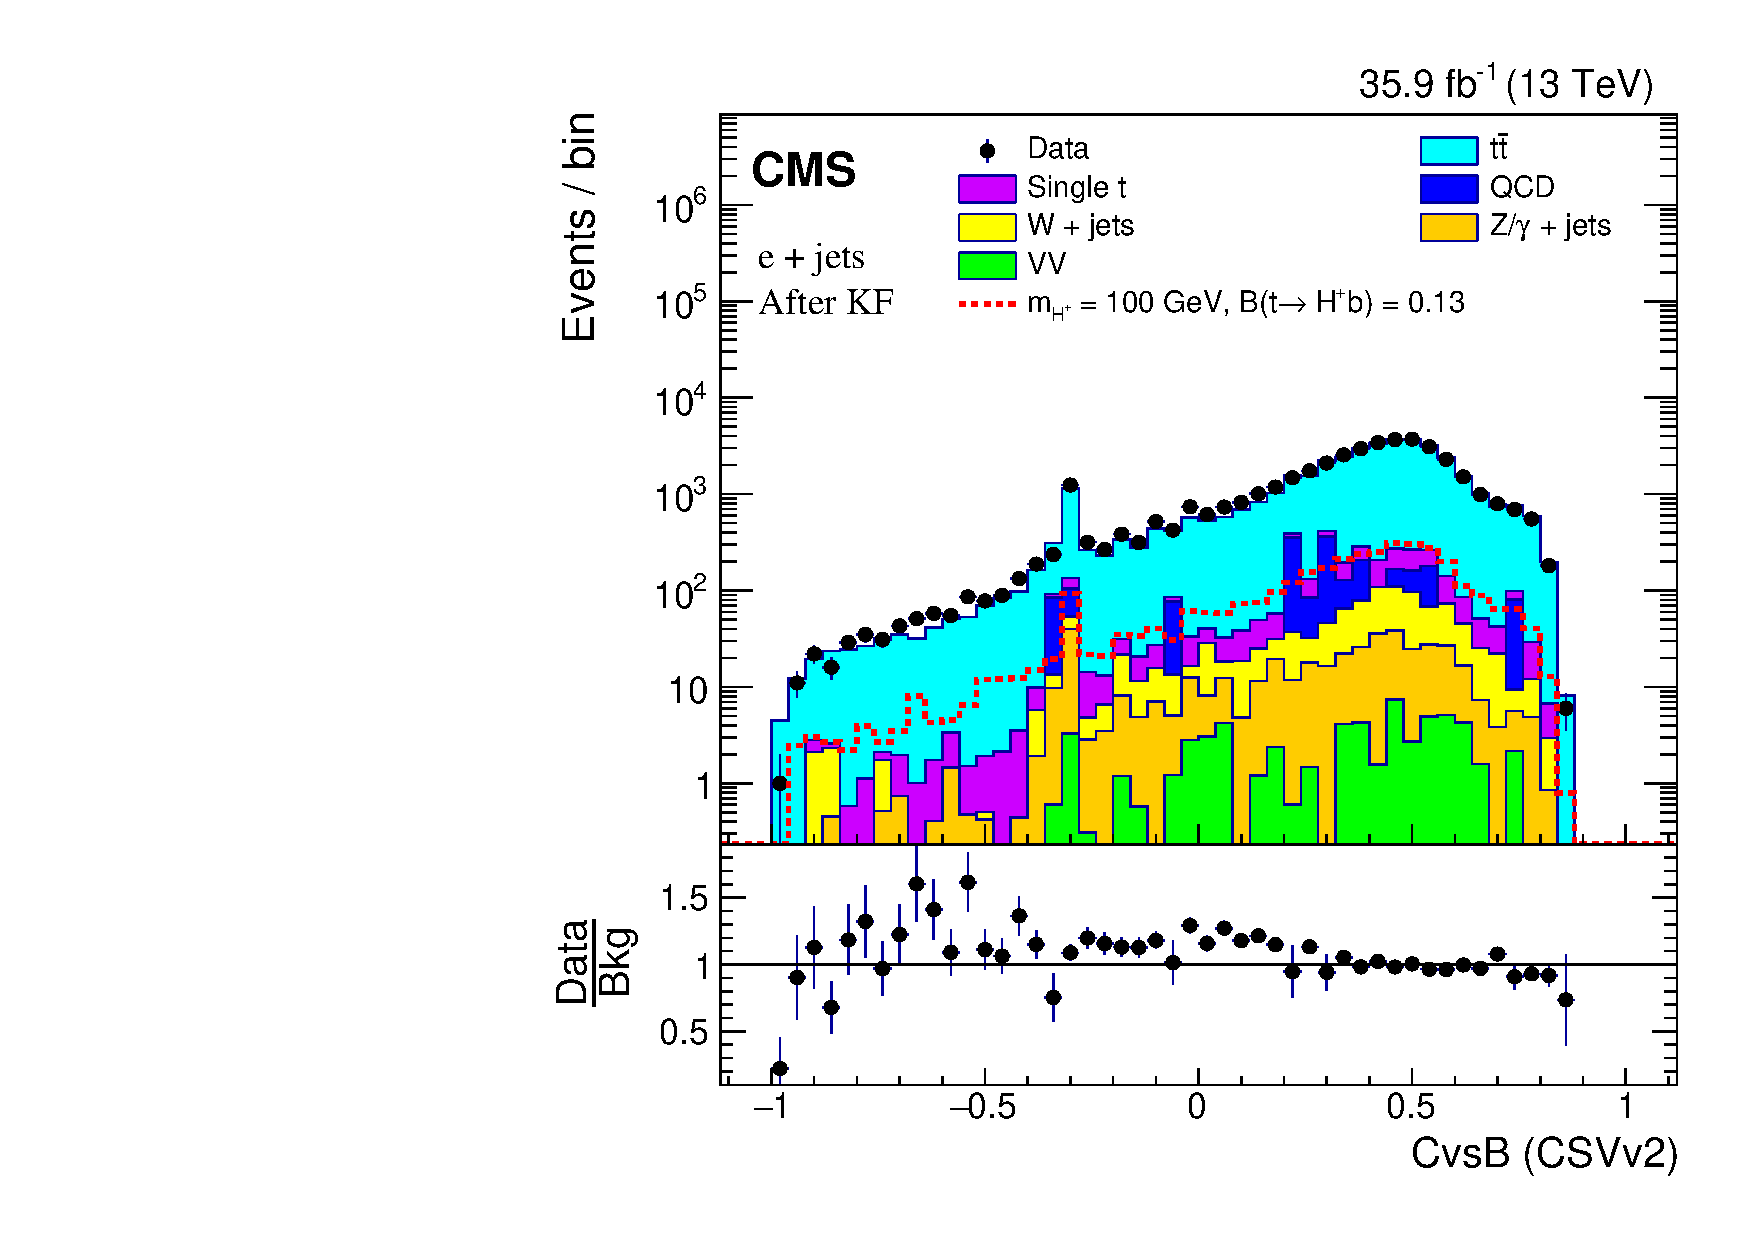
\includegraphics[width=0.50\linewidth]{Image/Electron/KinFit/pfCCvsB_eleKinFit.pdf}}
\vfil
\subfigure[charm vs. light jet discriminator ]{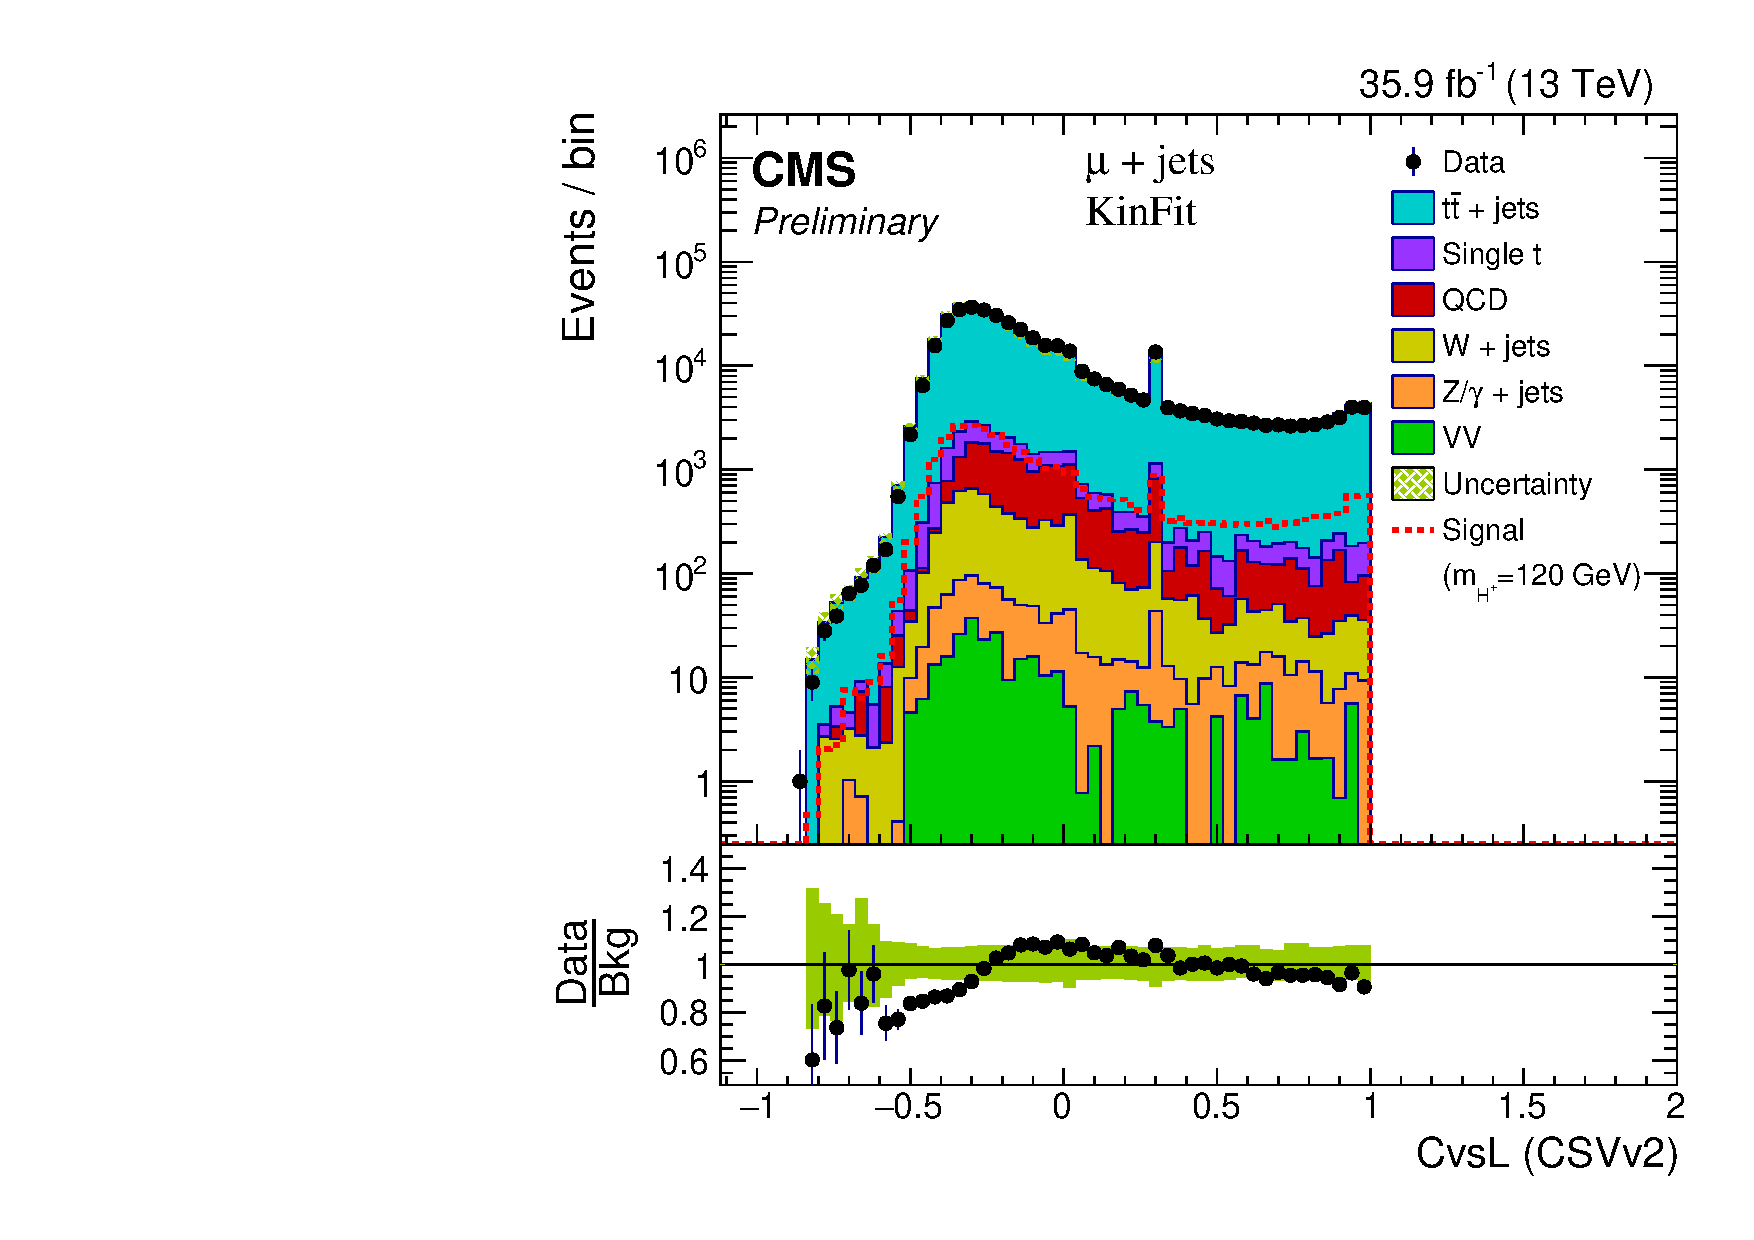
\includegraphics[width=0.50\linewidth]{Image/Muon/KinFit/pfCCvsL_muKinFit.pdf}}
\subfigure[charm vs. light jet discriminator ]{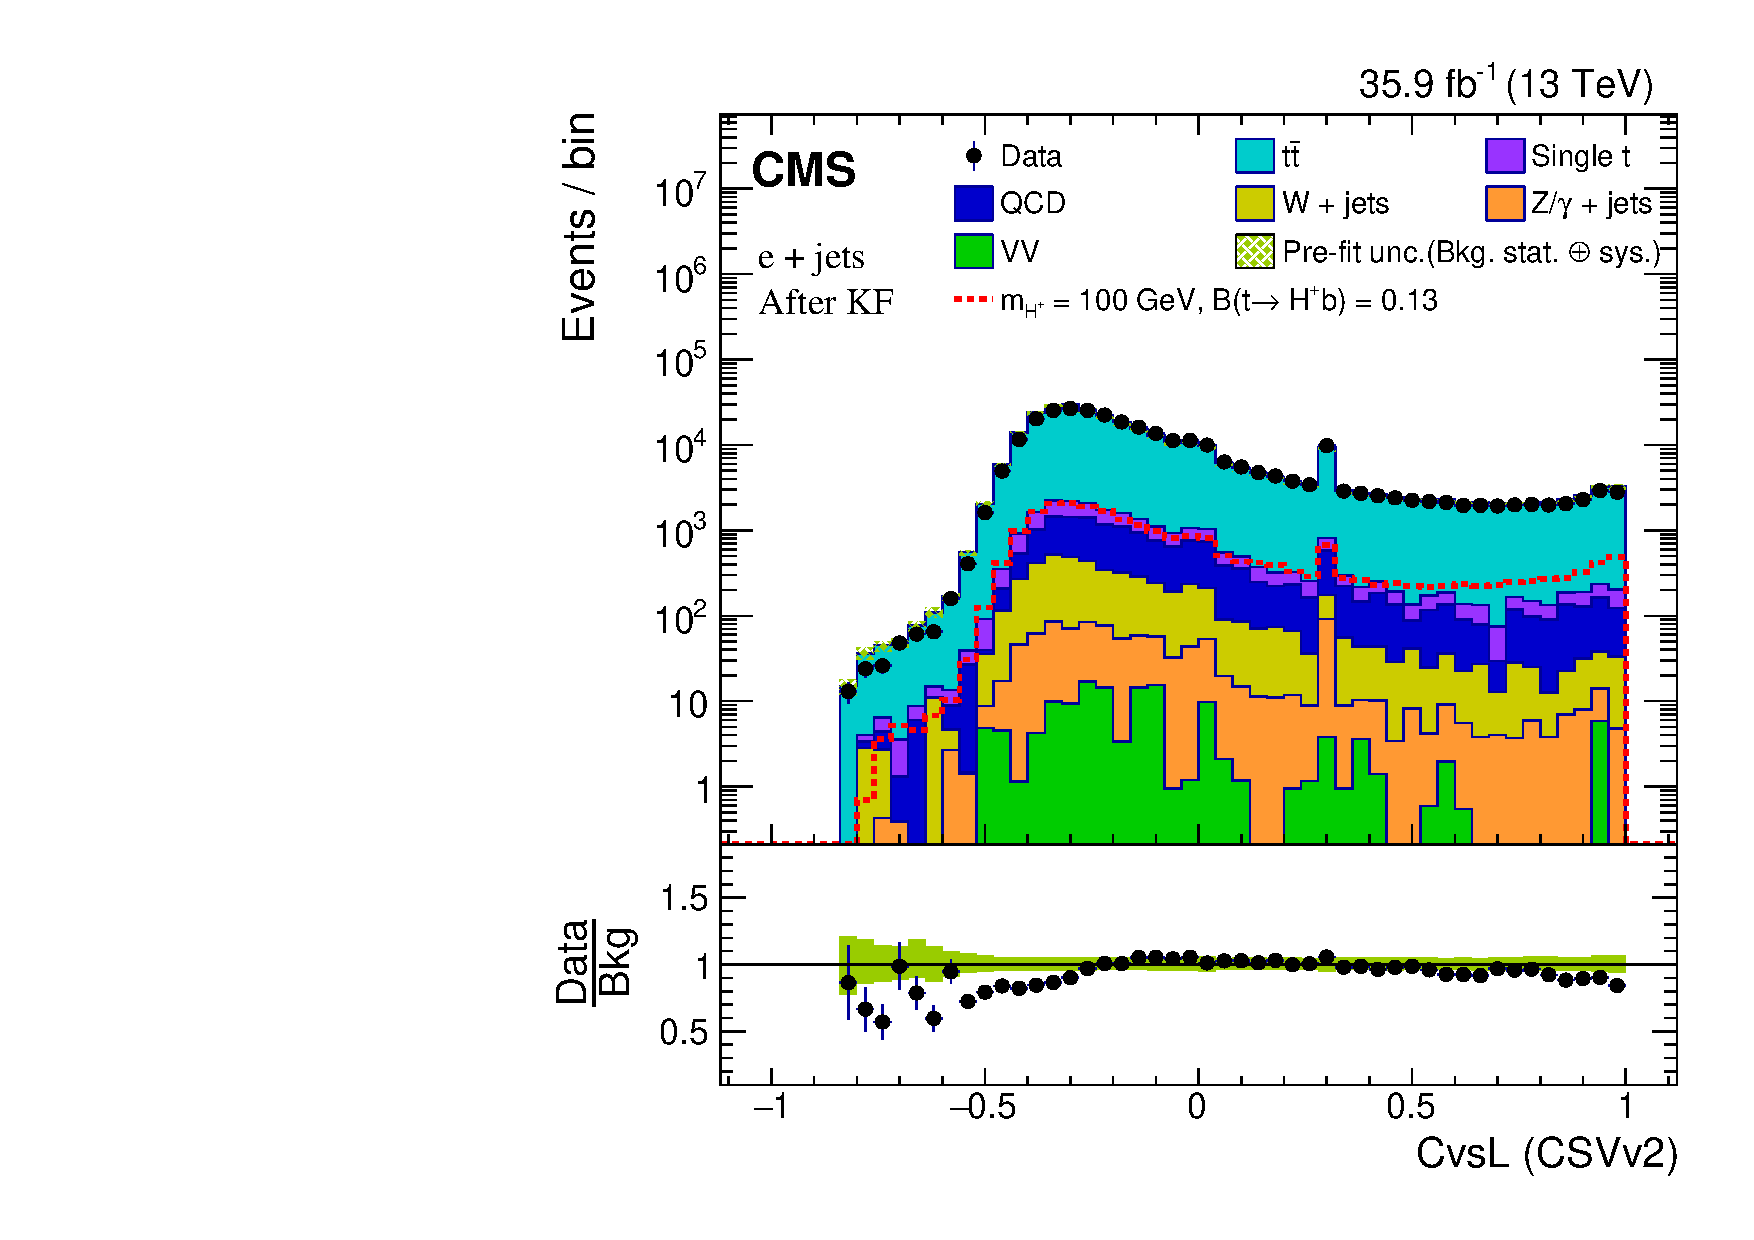
\includegraphics[width=0.50\linewidth]{Image/Electron/KinFit/pfCCvsL_eleKinFit.pdf}}
\caption{ The charm-discriminator distributions of two non-bjets after 
    kinematic fitting selection as described in Sec.~\ref{s:secEvtSel}, 
    obtained using the CSV method for the \mujets and \ejets channel.
    The jets with associated tracks not satisfying a set of selection criteria, 
    as listed in \cite{CMS-PAS-BTV-16-001}, are responsible for the spikes in 
    these distributions.} 
\label{fig:pfCCvsBL}
\end{figure}




%-------------------------------------
% Corrections on MC
%-------------------------------------
\newpage
\section{Corrections on MC}
\label{s:secMCSF}
\section{Luminosity scale factors}
\label{s:lumi_sf}

The simulated events listed in Table~\ref{tab:mcSample} are arbitrarily generated.
While comparing distributions obtained using simulated events with that of data, 
the former has to be normalised with the integrated luminosity of data.
To achieve this, each simulated sample is multiplied by the following luminosity scale 
factor ($\rm{SF}_{L}$):
\begin{equation}
\rm{SF}_{L}=\frac{L_{\rm {data}}}{L_{\rm {simulation}}} = \frac{L_{\rm {data}}\times\sigma_{\rm {simulation}}}{N_{\rm {simulation}}},
\label{eq:lumiSF}
\end{equation}
where $L_{\rm data}$ = 35.9\fbinv and $N_{\rm {simulation}}$ is the number of 
simulated events and $\sigma_{\rm {simulation}}$ is the corresponding cross section for 
the given sample. As can be seen from Table~\ref{tab:mcSample}, the $\rm{SF}_{L}$ value is less 
than 1 for most of the background samples except for QCD multijet. For QCD multijet samples, 
it is very large compared to other backgrounds owing to less number of generated events compared 
to its cross section. Simulation of large number of QCD multijet events is not feasible because of 
computing limitations.  

\section{Pileup reweighting}
\label{s:pileup_reweighting}
The pileup distributions in the data and simulation are different. To have the
same pileup distribution, the simulated events are reweighted. Depending on 
the number of primary vertices, the simulated event is multiplied by corresponding 
pileup weight. The pileup weights are the ratio of pileup distributions from 
data and simulation. 

\section{Lepton scale factors}
\label{s:lepton_sf}
Trigger, tracking, isolation and identification efficiencies are different between simulation and data.
A $\pt$ and $\eta$ dependent scale factors are applied to simulated events to take care of this 
difference. The muon scale factors are era dependent. There are different muon scale factors for era 
BCDEF and GH. However, electron scale factors are the same for full 2016 data taking period.
Separate scale factors are combined into one as
\begin{equation}
 \rm {SF}^\mu = \rm {SF}^\mu_{\rm {ID}}\times \rm {SF}^\mu_{\rm {iso}}\times \rm {SF}^\mu_{\rm {track}}\times \rm {SF}^\mu_{\rm {trig}}, \quad
 \rm {SF}^{ele} = \rm {SF}^{ele}_{\rm {ID}}\times \rm {SF}^{ele}_{\rm {reco}}\times \rm {SF}^{ele}_{\rm {trig}},
\label{eq:lepSF}
\end{equation}
where $\rm {SF}^\mu_{\rm {ID}}$, $\rm {SF}^\mu_{\rm {iso}}$, $\rm {SF}^\mu_{\rm {track}}$ and $\rm {SF}^\mu_{\rm {trig}}$ are weighted
average with luminosity ($L$) for different eras (BCDEF and GH) \eg 
\begin{equation}
 \rm {SF}^\mu_{\rm {ID}}=\frac{\rm {SF}^\mu_{\rm {ID}}({\rm {BCDEF}})\times L({\rm {BCDEF}})+\rm {SF}^\mu_{\rm {ID}}({\rm {GH}})\times L({\rm {GH}})}
 {L({\rm {BCDEF}})+L({\rm {GH}})},
\end{equation}
where, for example, $\rm {SF}^\mu_{\rm {ID}}({\rm {BCDEF}})$ is the scale factor for 
era-B to era-F and L({\rm {BCDEF}}) is the luminosity during this period. A similar formula 
for $\rm {SF}^\mu_{\rm {iso}}$, $\rm {SF}^\mu_{\rm {track}}$ and $\rm {SF}^\mu_{\rm {trig}}$ is used. The scale 
factors of Equation (\ref{eq:lepSF}) are applied on simulated events. 

\section{Jet and \MET correction}
\label{s:JEC}
Jets from simulations are smeared using jet energy scale (JES) and jet energy 
resolution (JER) to have the same resolution as that in data~\cite{Khachatryan:2016kdb}.
For smearing, $\pt$ and $\eta$ dependent scale factors are used as listed 
in Table~\ref{tab:jer_sf}. The $\pt$ of jet in simulations is scaled by the 
following factor:
\begin{equation}
    {\pt}_{\text{scale}} = {\rm {max}}[0.0,1.0+(\rm{SF}-1)\times({\pt}_{\text{jet}}-{\pt}_{\text{jet}}^{\text{gen}})/{\pt}_{\text{jet}}]
\end{equation}
with the following constraint:
\begin{equation}
    {\pt}_{\text{jet}}^{\text{gen}}> 0, \quad \Delta \rm R<0.2, \quad |{\pt}_{\text{jet}}-{\pt}_{\text{jet}}^{\text{gen}} |<
    3\times\sigma_{\rm {JER}}\times{\pt}_{\text{jet}},
\end{equation}
where $\Delta \rm R$ is the angular separation between the reconstructed and 
generated jet and $\sigma_{\text{JER}}$ is resolution of \pt of reconstructed jet. 
\begin{table}
    \caption{Jet energy resolution scale factors for different $\eta$ range}
 \label{tab:jer_sf}
 \begin{center}
 \begin{tabular}{cccc}
     \hline
     \hline
     $\eta$ range & base & down & up \\ 
     \hline
     \hline
     $0.0 \leq | \eta |< 0.5 $ & 1.109 & 1.044 & 1.174 \\
     $0.5 \leq | \eta |< 0.8 $ & 1.138 & 1.072 & 1.204 \\
     $0.8 \leq | \eta |< 1.1 $ & 1.114 & 1.050 & 1.178 \\
     $1.1 \leq | \eta |< 1.3 $ & 1.123 & 1.022 & 1.224 \\
     $1.3 \leq | \eta |< 1.7 $ & 1.084 & 0.985 & 1.183 \\
     $1.7 \leq | \eta |< 1.9 $ & 1.082 & 0.973 & 1.191 \\
     $1.9 \leq | \eta |< 2.1 $ & 1.140 & 1.020 & 1.260 \\
     $2.1 \leq | \eta |< 2.3 $ & 1.067 & 0.953 & 1.181 \\
     $2.3 \leq | \eta |< 2.5 $ & 1.177 & 0.967 & 1.387 \\
     $2.5 \leq | \eta |< 2.8 $ & 1.364 & 1.203 & 1.525 \\
     $2.8 \leq | \eta |< 3.0 $ & 1.857 & 1.654 & 2.060 \\
     $3.0 \leq | \eta |< 3.2 $ & 1.328 & 1.203 & 1.453 \\
     $3.2 \leq | \eta |< 5.0 $ & 1.160 & 1.013 & 1.307 \\ \hline
 \end{tabular}
 \end{center}
 \end{table}

\section{\text{b} tag scale factor}
\label{s:bTagSF}
The \PQb tagging efficiency is different between simulation and data.
An event weight as given by Equation (\ref{eq:btagWt}) is applied on the simulated events to 
take care of this difference ~\cite{BTagSFMethods}. 
\begin{equation}
P(\text{Simulation}) = \prod_{\text{i = tagged}} \epsilon_i \prod_{\text{j = not tagged}}(i -\epsilon_j)
\end{equation}
\begin{equation}
P(\text{Data}) = \prod_{\text{i = tagged}} \text{SF}_{i}\epsilon_i \prod_{\text{j = not tagged}} (1-\text{SF}_j\epsilon_j)
\end{equation}
\begin{equation}
w = \frac{P(\text{Data})}{P(\text{Simulation})}
\label{eq:btagWt}
\end{equation}
 The \PQb tagging efficiency $\epsilon_f(m,n)$ in the $(m,n)$ bin of $\pt$ and $\eta$ is calculated 
 using the following formula                                                               
 \begin{equation}                                                                          
  \epsilon_f(m,n)=\frac{N^{\rm {\PQb-tagged}}_f(m,n)}{N^{\rm {total}}_f(m,n)},                   
 \label{eq:btag_eff}                                                                       
 \end{equation}                                                                            
 where $N^{\rm {\PQb-tagged}}_f(m,n)$ is the number of \PQb-tagged jets with flavor \text{f}
(\PQb quark, \PQc quark, light quark, and gluon) and $N^{\rm {total}}_f(m,n)$ is the total number 
of events. The scale factor ($\text{SF}_i$) depends on $\pt$, $\eta$, parton flavor of jet, and 
\PQb jet discriminator value. 



%-------------------------------------
% Event filters and triggers
%-------------------------------------
\newpage
\section{Event Filters and Triggers}
\label{s:secFilters}
\subsection{Filters}
A series of filters as recommended by the JetMET POG \cite{metFilters} are applied to
filter "bad" events, such as those where there is a huge difference in the \pt of
muon measured from the tracker and the muon chambers. Although the occurrence of such
"bad" events is rare, these filters are applied as sanity measures. These
filters mostly affect the actual data, most of them have no effect on the simulated
events. The efficiency of all combined filters is 99.4\% for data, and 99.9\%
for SM \ttjets MC sample. These filters are particularly useful in those
analyses where there is a requirement of very high missing transverse energy (MET)
and the final event yield is small. A detailed description of each filter is given
below:
\begin{itemize}
	\item \textbf{HBHE noise filter}: It is known that the barrel and endcap
		part of the HCAL records noise (sporadic anomalous signals) at a
		fixed
		rate even if there is no stable beam for physics data taking
        \cite{metFilters}. An event is supposed to have such a noise if the flag
		\verb|Flag_HBHENoiseFilter| is set to 1. Such an event is filtered.
	\item \textbf{HBHE isolated noise filter}: This filter first finds the
		candidates for rechits and rejects the event if the sum of
		iso-tagged energy is $>$ 50 GeV, the sum of iso-tagged transverse
		energy
		$>$ 25 GeV, and the number of iso-tagged rechits is $>$ 9. The flag
		\verb|Flag_HBHENoiseIsoFilter| is used for this purpose.
 	\item \textbf{CSC beam halo filter}: The actual physics objects of interest
		are those which are produced in the pp collision. However, there
		are machine induced particles, produced through beam-gas or
		beam-pipe interactions, which fly with the beam at a large radius
		(up to 5m). These machine induced particles are reconstructed mainly
		in the Cathode Strip Chambers (CSC) as muon candidate. A set of
		selection is applied through
        \verb|Flag_globalSuperTightHalo2016Filter| \cite{metFilters}. This flag is
		set to 1 if the CCS beam halo filter is applied and 0 if not applied.
	\item \textbf{Good primary vertex filter}: The events are required to have
		at least one good primary vertex. Therefore, those events are
		filtered where there is no good vertex. A good vertex is
		required to be real, the z-component of the position is $ <$ 24 cm,
		the $\rho$ component of the position $<$ 2 cm, and the minimum
		number of degrees of freedom are $>$ 4. The \verb|Flag_goodVertices|
		is set to 1 if the event has passed this filter.
	\item \textbf{Bad EE supercrystal filter}: The events are filtered if
		there is an unusually large energy deposit in the four superclusters
        of ECAL endcaps \cite{metFilters}. This filter is applied only on data
		through the \verb|Flag_eeBadScFilter|.
	\item \textbf{ECAL dead cell trigger primitive filter}: If the energy of
		the ECAL crystals are estimated from the trigger primitive and
		lies near the saturation energy then that event is filtered
        \cite{metFilters}. The \verb|Flag_EcalDeadCellTriggerPrimitiveFilter| flag
		is used to indicate if an event passes this filter or not.
	\item \textbf{Bad PF muon filter}: An event is filtered if the muon is
		although qualified as a PF muon but the quality is very low, and
		the \pt is large. The events are filtered if a muon is found
		which has \pt $>$ 100 GeV, segment compatibility $< 0.3$ or relative
		percentage error in the \pt of the best (inner) track is more than
		200\% (100\%), and $\Delta R$ (muon, PFmuon) $< 0.001$.
	\item \textbf{Bad charged hadron filter}: Those events are filtered where
		the quality of the muon is low and it is not declared as PF muon.
		However, this non-PF muon is used in the calculation of PF-MET
		as a candidate for charged hadron. To reject such events, the muon
		is required to have same \pt, segment compatibility, and error in
		track cuts as that of the above filter. An additional requirement
    of $\Delta R$ (muon, charge hadron) $<$ 0.00001, and \verb|PtDiffRell|
		$< 0.00001$ is applied where \verb|PtDiffRell| = (\pt of PF candidate - \pt
		of muon inner track)/(0.5* (\pt of PF candidate + \pt of muon inner
		track)).
\end{itemize}

All of the above filters are not directly stored in the trigger collection of the
\verb|MINIAOD| data set. The \verb|EDFilters| are used on the fly to apply unavailable
filters. The list of filters with their availability and pplicability is shown
in Table (\ref{tab:eventFilters}).
\begin{table}
\caption{ List of event filters applied to data and MC samples. Most of the filters
	are available in the {\em MINIAOD} through the trigger collection. The
	unavailable filters are applied on the fly using EDFilters.}
\label{tab:eventFilters}
\centering
\begin{adjustbox}{max width=\textwidth}
 \begin{tabular}{ccc}\hline\hline
  {\bf{Name of the filter}} & {\bf{Available in MINIAOD}} & {\bf{Applied on}}\\\hline\hline
  \verb|HBHE noise filter|            & Yes & Data \& MC \\
  \verb|HBHE isolated noise filter|   & Yes & Data \& MC \\
  \verb|CSC beam halo filter|         & Yes & Data \& MC \\
  \verb|Good primary vertex filter|   & Yes & Data \& MC \\
  \verb|Bad EE supercrystal filter|   & Yes & Data  \\
  \verb|ECAL dead cell trigger primitive filter| & Yes & Data \& MC\\
  \verb|Bad PF Muon Filter|  & No & Data \& MC \\
  \verb|Bad Charged Hadron Filter|        & No & Data \& MC \\\hline
 \end{tabular}
\end{adjustbox}
\end{table}


\subsection{Triggers}
The high-level triggers (HLT) are applied to select events enriched
with desired physics objects. The trigger conditions are stored in the form of
programming strings also called trigger paths. For every event, these paths are
stored. Depending on the topology of an analysis, an event is selected if the
corresponding trigger path is available in that event. For this analysis, an
event is selected if it has a trigger path of \verb|HLT_IsoMu24*| and
\verb|HLT_IsoTkMu24*| with logical \verb|OR| for the muon channel, and
\verb|HLT_Ele27_WPTight_Gsf| for electron channel. The efficiency of these
triggers depends on \pt and $\eta$ of the lepton. For lower Pt, the efficiency is
very poor and has a sudden increase at a particular value. That sudden increase is called trigger turn-on and the leptons are required to have \pt higher than that at the
turn-on.

The muon and electron trigger efficiency as a function of \pt is shown in Figure
(\ref{fig:trigEff}). The trigger turn-on for muon trigger is at about \pt = 24 GeV,
hence in the
subsequent selection, the muon is required to have \pt $>$ 26 GeV. For the electron
trigger (\verb|HLT_Ele27_WPTight_Gsf|), the trigger turn-on is a little higher at about
\pt = 33 GeV, therefore a cut of \pt $>$ 35 GeV is applied on electrons in the
subsequent selection.
\begin{figure}
     \centering
	\subfigure[Muon trigger efficiency \cite{ref:muon-twiki}]
     	{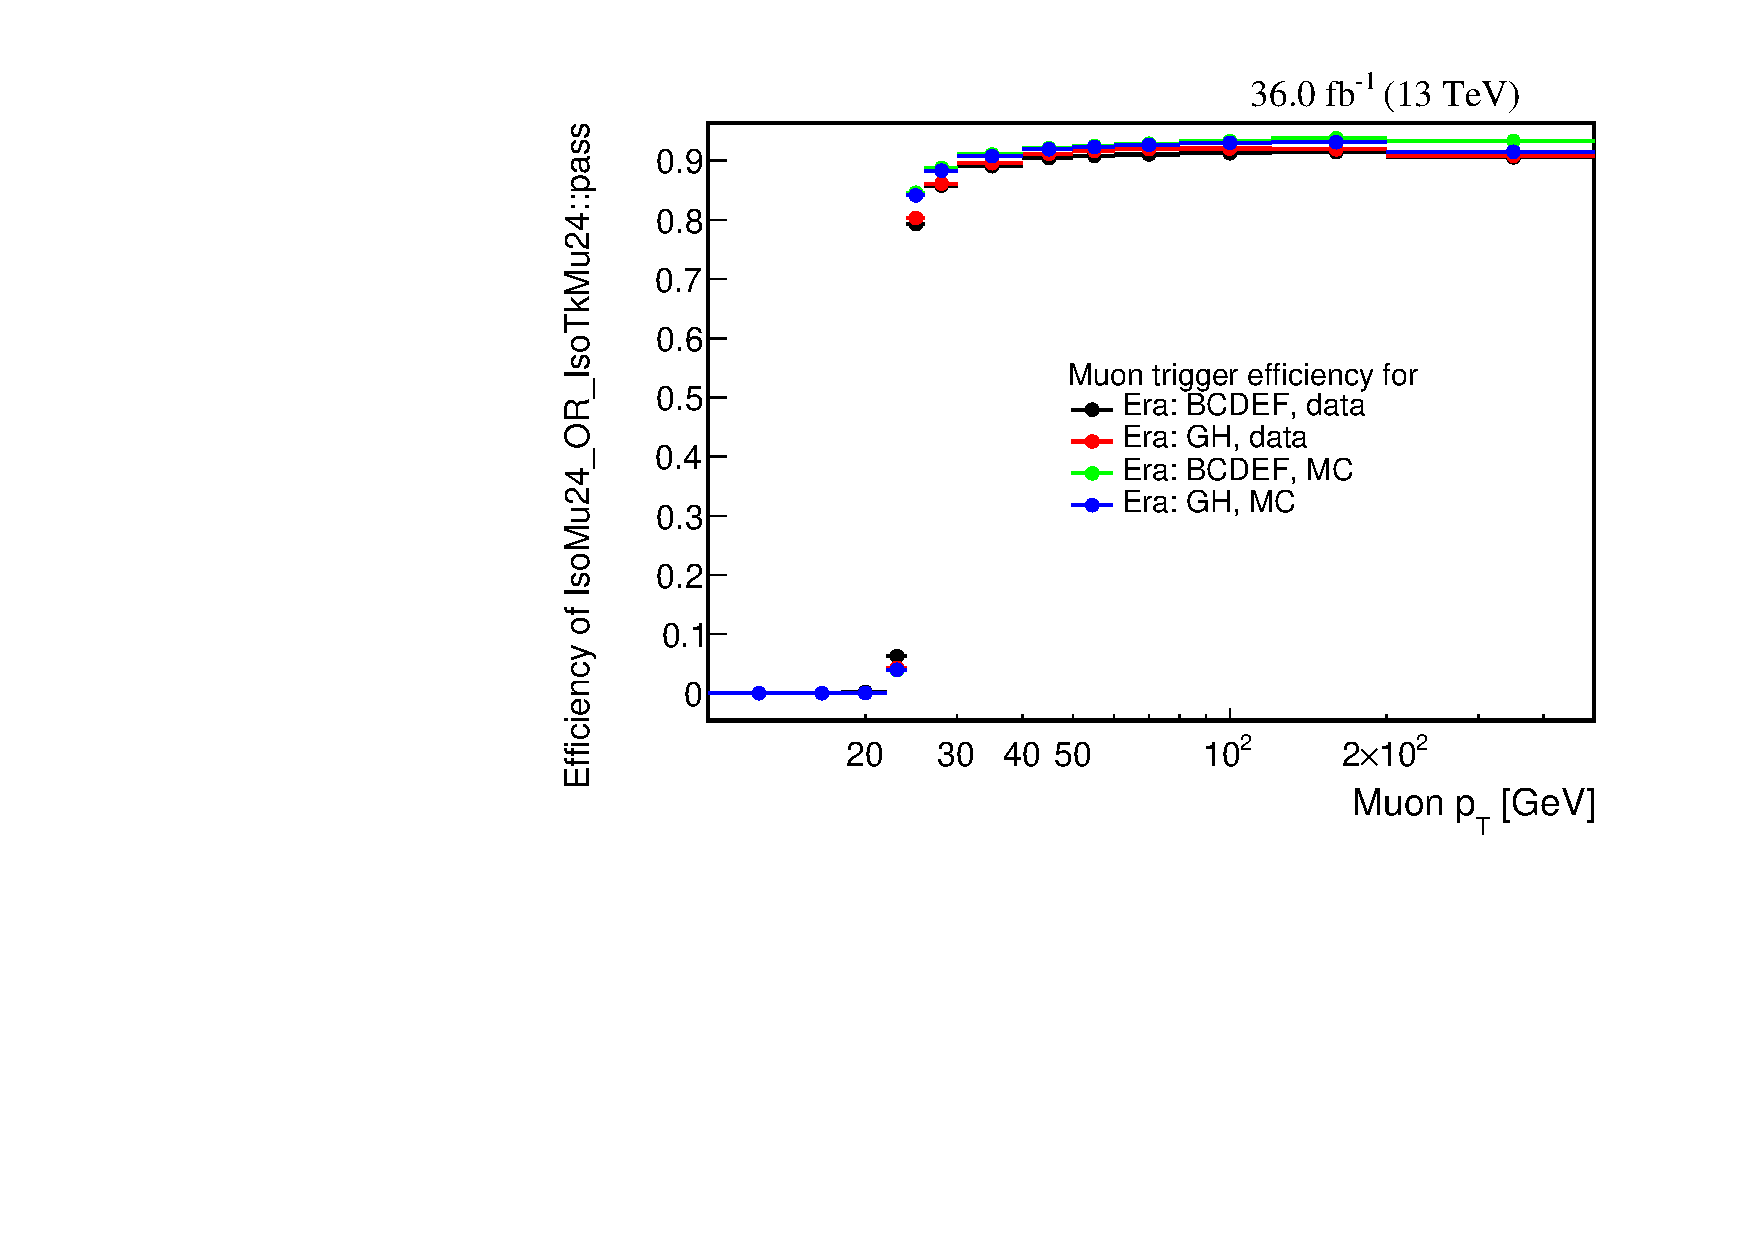
\includegraphics[width=0.60\linewidth]{Image/EffAndSF/muonTrigEff.pdf}}
     	\vfil
	\subfigure[Electron trigger efficiency in the barrel region \cite{eleTrigEff}]
     	{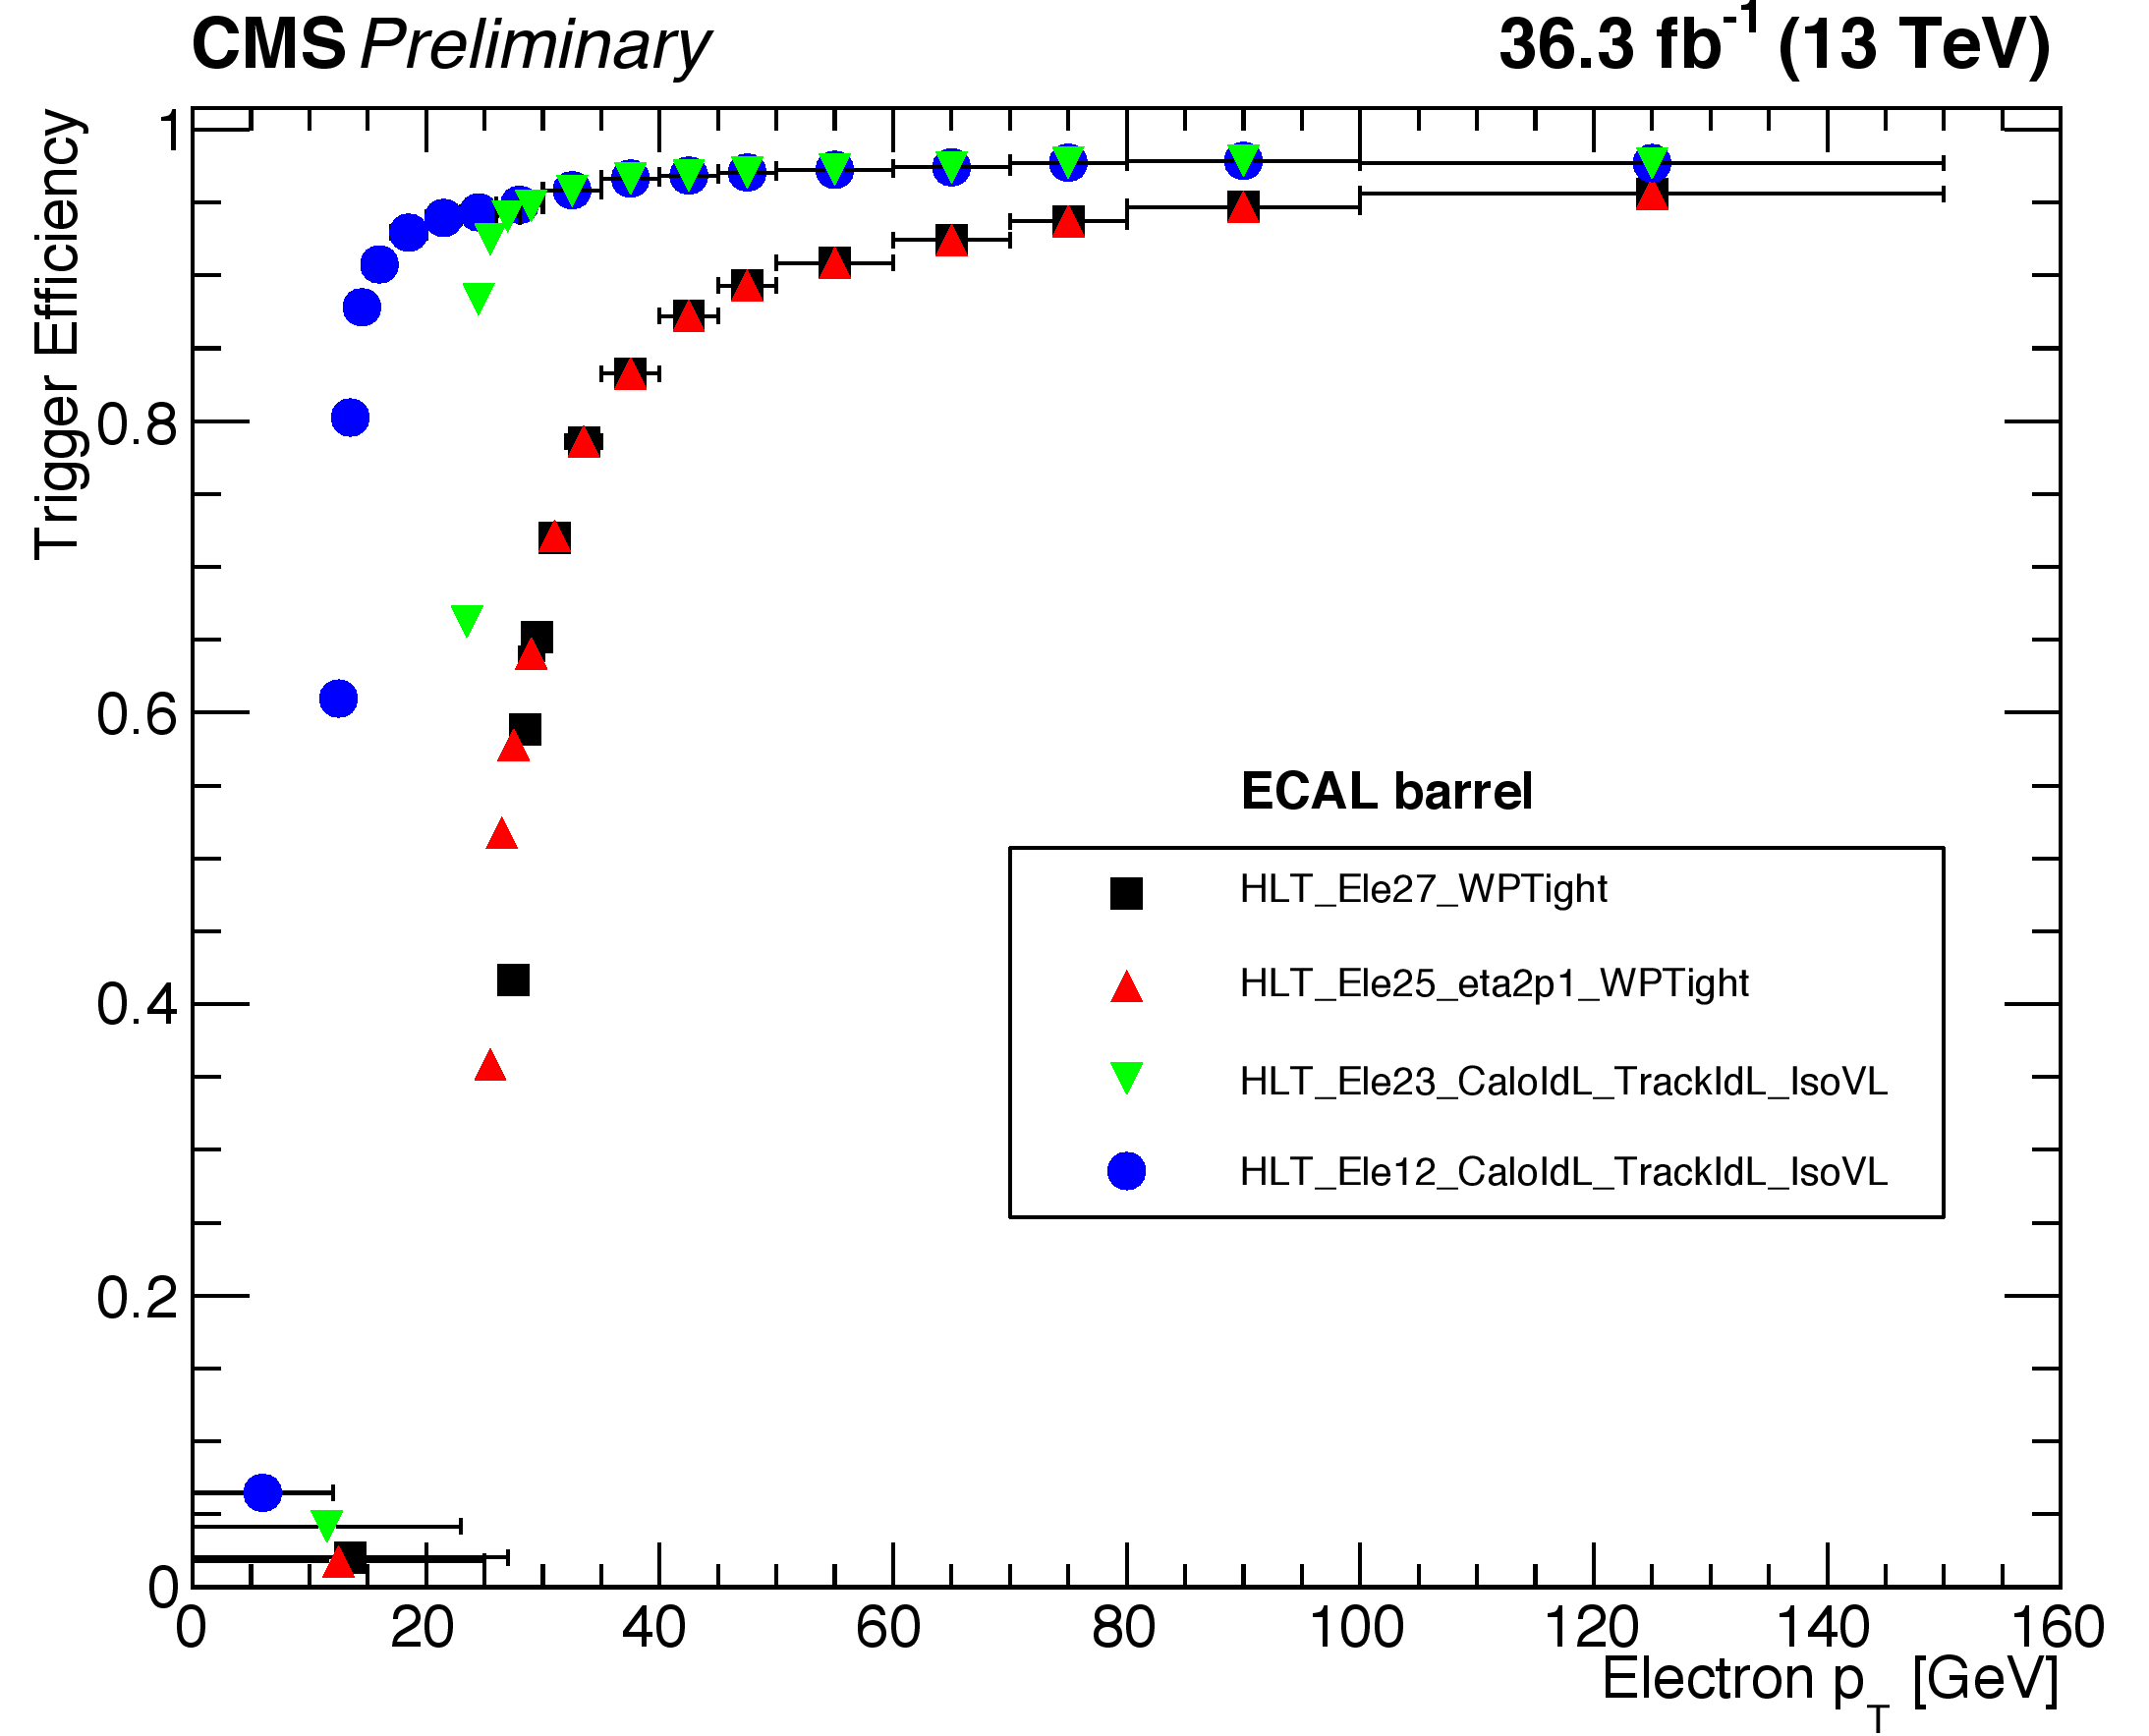
\includegraphics[width=0.49\linewidth]{Image/EffAndSF/eleTrigEB.png}}
	\subfigure[Electron trigger efficiency in the endcap region \cite{eleTrigEff}]
     	{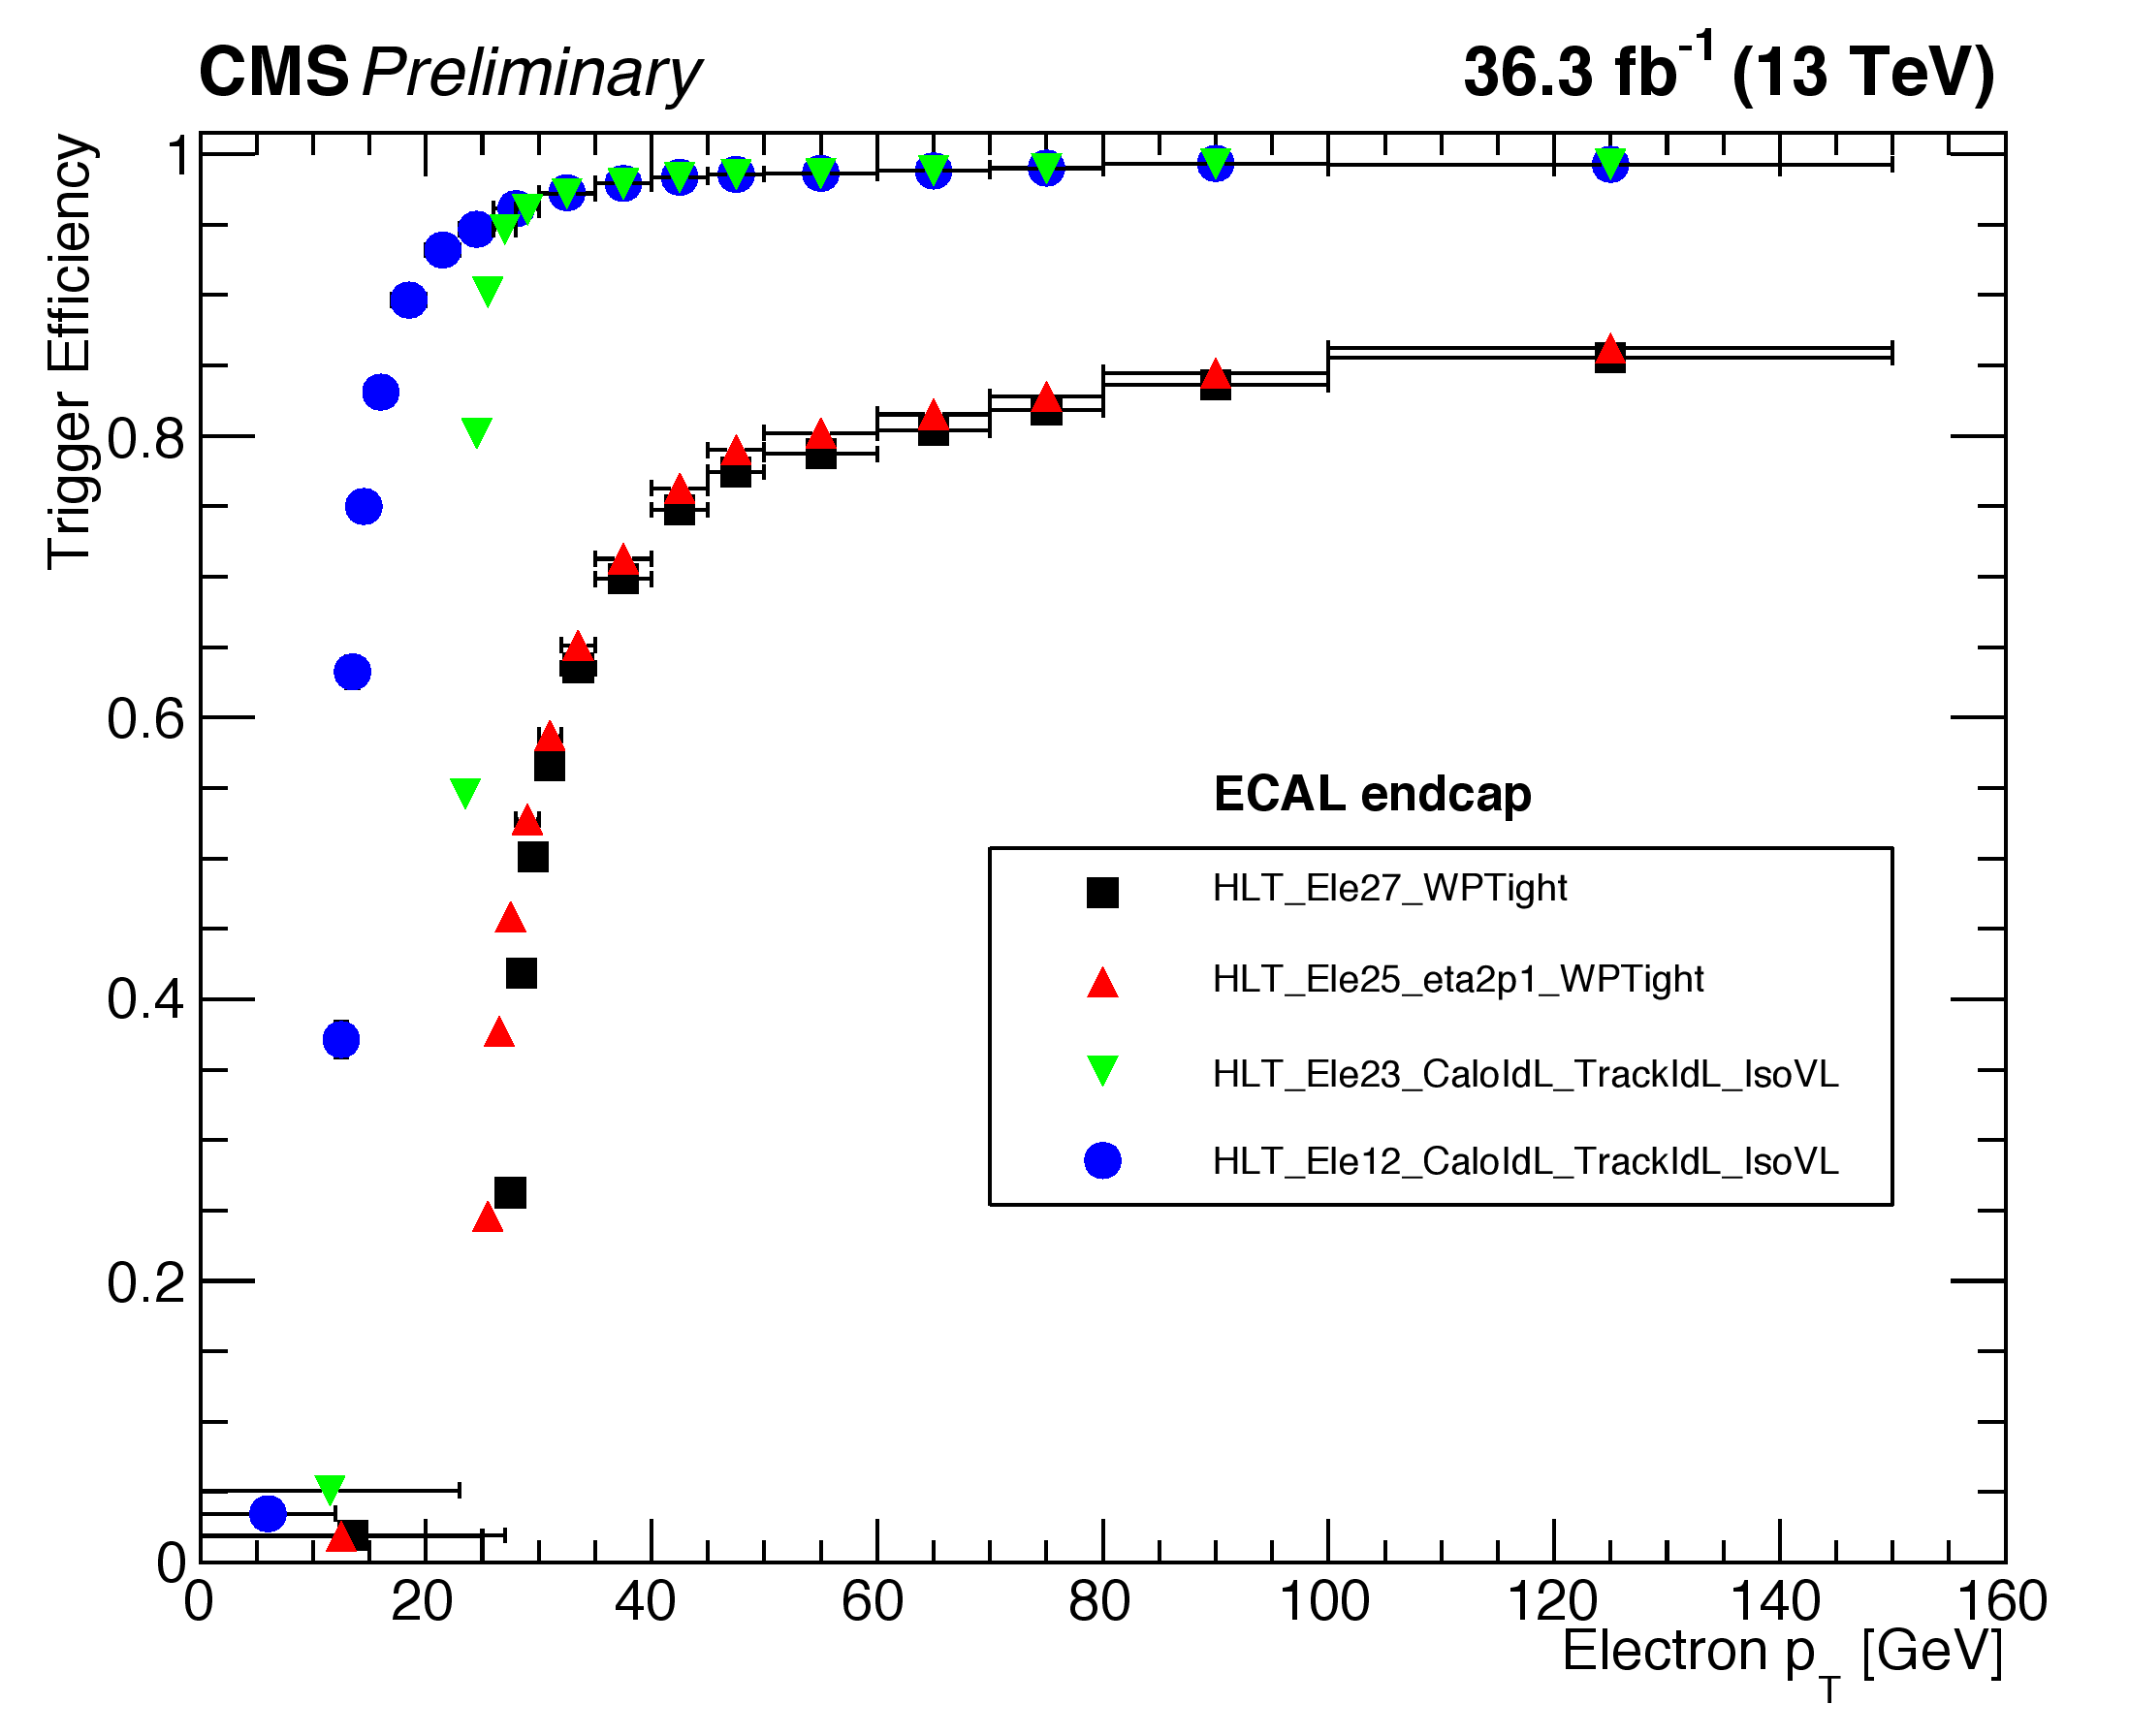
\includegraphics[width=0.49\linewidth]{Image/EffAndSF/eleTrigEE.png}}
	\caption{Muon and electron trigger efficiency as a function of transverse
	momentum. The trigger turn-on is at about \pt = 24 GeV for muon, and 33 GeV
	for electron (HLT\_Ele27\_WPTight\_Gsf) triggers.}
     \label{fig:trigEff}
 \end{figure}


%-------------------------------------
% Event Selection
%-------------------------------------
\section{Event Selection}
\label{s:secEvtSel}

In the final state, there are four jets, one charged lepton and \MET.
Various selections cuts are applied to ensure the resulting events to have 
this topology. Cutflow plots after various selection cuts are shown in 
Figure~\ref{fig:cutflow}. Below we list out various selection requirements applied.
\begin{enumerate}[leftmargin=*]
\item{\bf{Event filter and trigger}}:
    The events are passed to the filters and triggers (Section~\ref{ss:secTrig}). 
    The lepton trigger is used to enrich events with lepton and significantly reduces QCD multijet 
    compared to other SM background. The number of events surviving filters and trigger cuts for 
    simulated signal and background and data are shown in the 2nd column of Tables
\ref{tab:cutflow_mu}, \ref{tab:cutflow_ele}, \ref{tab:cutflow_mu_sig} and \ref{tab:cutflow_ele_sig}. 
\item {\bf{Lepton selection}}:
The event topology has only one lepton thus events having a second loose lepton are not selected. 
The lepton-veto selection for the \mujets and \ejets channel are listed in Tables~\ref{tab:muonSel}
and \ref{tab:eleSel}.
For the \mujets (\ejets) channel there cannot be any electron (muon) in an event.
Those events where there is any electron (muon) in the \mujets (\ejets) channel are rejected.
Lepton scale factors as described in Section~\ref{s:lepton_sf} are applied to the simulated events.
The relative isolation cut for muon is $I_{\rm {rel}}^{\mu} < 0.15$ and for electron it is 
$I_{\rm {rel}}^{\rm{e}} < 0.0821 (0.0695)$ in the barrel (endcap) region.
Event yields after one lepton selection are shown in the 3rd column of Tables~\ref{tab:cutflow_mu},
\ref{tab:cutflow_ele}, \ref{tab:cutflow_mu_sig} and \ref{tab:cutflow_ele_sig}.

\item {\bf{Jet selection}}:
There should be at least four jets in an event.
Jet selection cuts are listed in Table~\ref{tab:jetSel}.
The jet energy is corrected using JES and JER scale factors.
After correcting jet energy, the selections on jet as shown in Table~\ref{tab:jetSel} are applied.
Number of events after jet selection are shown in the 4th column of Tables~\ref{tab:cutflow_mu},
\ref{tab:cutflow_ele}, \ref{tab:cutflow_mu_sig} and \ref{tab:cutflow_ele_sig}.

\item {\bf{\MET selection}}:
The missing transverse energy should be greater than 20 \GeV. Event yields after \MET selection are 
shown in the 5th column of Tables~\ref{tab:cutflow_mu}, \ref{tab:cutflow_ele}, \ref{tab:cutflow_mu_sig}
and \ref{tab:cutflow_ele_sig}. After applying \MET selection QCD multijet, \dyjets event yields reduce 
more compared to \ttjets, single \PQt, \wjets, and VV processes as there is no neutrino at the parton level.

\item {\bf{\text{b} jet selection}}:
For \PQb jet selection, the medium working point is used i.e, $b_{\text{discr}} > 0.8484$. 
The \PQb tag event weights, as described in Section~\ref{s:bTagSF}, are applied on simulated events. 
The events are required to have at least two \PQb jets. Event yields for simulated signal, background 
and data are shown in the 6th column of Tables~\ref{tab:cutflow_mu}, \ref{tab:cutflow_ele}, 
\ref{tab:cutflow_mu_sig} and \ref{tab:cutflow_ele_sig}.
\end{enumerate}

From Table~\ref{tab:cutflow_mu} (\ref{tab:cutflow_ele}) it can be seen that the \wjets 
process is the dominant background upto 1-lepton selection. However, when the events are 
required to have $N_{\rm{jets}} \geq 4$, the \ttjets becomes the dominant background. The \ttjets 
remains dominant background after subsequent selection cuts. The QCD multijet events are from
simulated samples as shown in Table~\ref{tab:mcSample}. The signal event yields for a different 
mass of charged Higgs after various selection cuts are shown in Table~\ref{tab:cutflow_mu_sig}
(\ref{tab:cutflow_ele_sig}) for the \mujets (\ejets) channel. It can be seen from these tables 
that the event yields are almost the same upto 1-lepton selections for all masses of charged Higgs. 
However, after the $N_{\text{jets}} \geq 4$ selection, when \ttjets becomes the dominant 
background as shown in Table~\ref{tab:cutflow_mu} (\ref{tab:cutflow_ele}), the event yield 
for higher masses of the charged Higgs are reduced more compared to lower masses. The 
event yield reduces because of the less phase space available between \PQt quark and charged 
Higgs for higher masses.
    
\begin{center}
\begin{figure}
\subfigure[]{\includegraphics[width=0.50\linewidth]{Image/Muon/cutflow_mu.pdf}}
\subfigure[]{\includegraphics[width=0.50\linewidth]{Image/Electron/cutflow_ele.pdf}}
\caption{ Event yields after various selection cuts for the \mujets and \ejets channel.} 
\label{fig:cutflow}
\end{figure}
\end{center}

\begin{table}
\begin{center}
    \caption{Event yields after various selection cuts for the \mujets
    channel. The \wjets process is the dominant background upto 1-lepton 
    selection. When the events are required to have $N_{\text{jets}} \geq 4$, the 
    \ttjets becomes the dominant background. The QCD multijet events are 
    from simulated samples as listed in Table~\ref{tab:mcSample}. The simulated 
    MC signal process corresponds to $\mHp=120$ \GeV.}
\label{tab:cutflow_mu}
\begin{adjustbox}{max width=\textwidth}
\begin{tabular}{cccccccc}
\hline 
\hline 
\multicolumn{1}{ c}{Process } & \multicolumn{1}{ c}{ Trigger } & \multicolumn{1}{ c}{ $N_{\mu}=1$ } &\multicolumn{1}{ c}{ $N_{\rm{jets}}\ge 4$ } & \multicolumn{1}{ c}{ $\MET \ge $ 20\GeV }&  \multicolumn{1}{ c }{ $\ge$ 2 \PQb jets }& \multicolumn{1}{ c}{KF selection } & \multicolumn{1}{ c}{ $\ge$1 \PQc jet} \\ 
\hline 
\hline 
MC signal & 232088 & 182966 & 107237 & 97792 & 32309 & 15719.1 & 15784.7 \\ 
\hline 
SM \ttjets & 4.02837e+06 & 2.6683e+06 & 1.36181e+06 & 1.24994e+06 & 411521 & 191136 & 190228 \\ 
Single \PQt & 589196 & 428074 & 81804 & 74924.6 & 16599.5 & 5311.76 & 5272.39 \\ 
\wjets & 3.09765e+08 & 2.44546e+08 & 894318 & 797849 & 11767.7 & 2795.35 & 2760.97 \\ 
\dyjets & 4.48481e+07 & 1.27487e+07 & 73347.7 & 59133.7 & 1272.68 & 389.494 & 377.772 \\ 
QCD multijet & 1.4453e+08 & 4.07546e+07 & 355254 & 265303 & 11962.6 & 3007.9 & 2960.23 \\ 
VV & 653661 & 433207 & 17232.4 & 15614.6 & 440.143 & 146.569 & 146.862 \\ 
\hline 
Bkg & 5.04414e+08 & 3.01579e+08 & 2.78377e+06 & 2.46276e+06 & 453564 & 202787 & 201746 \\ 
\hline 
Data & 4.69828e+08 & 3.02791e+08 & 2.91052e+06 & 2.58346e+06 & 475011 & 203209 & 201361 \\ 
\hline 
Data/Bkg & 0.931433 & 1.00402 & 1.04553 & 1.04901 & 1.04729 & 1.00208 & 0.998092 \\ 
\hline 
\end{tabular}
\end{adjustbox}
\end{center}
\end{table}

\begin{table}
\begin{center}
    \caption{Event yields after various selection cuts for the \ejets channel. A similar trend as 
that of Table~\ref{tab:cutflow_mu} is seen. The simulated MC signal process corresponds to $\mHp=120$ \GeV.}
\label{tab:cutflow_ele}
\begin{adjustbox}{max width=\textwidth}
\begin{tabular}{cccccccc}
\hline 
\hline 
\multicolumn{1}{ c}{Process } & \multicolumn{1}{ c}{ Trigger } & \multicolumn{1}{ c}{ $N_{\rm {e}}=1$ } &\multicolumn{1}{ c}{ $N_{\rm{jets}}\ge 4$ } & \multicolumn{1}{ c}{ $\MET \ge 20 \GeV$ }&  \multicolumn{1}{ c }{ $\ge$ 2 \PQb jets }& \multicolumn{1}{ c}{KF selection} & \multicolumn{1}{ c}{$\ge$1 \PQc jet} \\ 
\hline 
\hline 
MC signal & 176709 & 143701 & 83955.8 & 76103.8 & 24488.2 & 11805.2 & 11835.4 \\ 
\hline 
SM \ttjets & 3.00511e+06 & 2.04055e+06 & 1.03705e+06 & 949027 & 306375 & 141807 & 141111 \\ 
Single \PQt & 436844 & 314868 & 63532.5 & 57857.3 & 12741.7 & 3988.54 & 3953.51 \\ 
\wjets & 1.95739e+08 & 1.34112e+08 & 660657 & 586662 & 8878.8 & 2031.55 & 1991.47 \\ 
\dyjets & 3.38256e+07 & 9.13592e+06 & 91830.9 & 68347.4 & 1449.81 & 433.03 & 418.256 \\ 
QCD multijet & 2.05104e+08 & 3.2298e+07 & 595856 & 453793 & 13497.6 & 9678.07 & 9613.93 \\ 
VV & 479881 & 298702 & 14058.6 & 12404.1 & 270.078 & 70.432 & 70.2293 \\ 
\hline 
Bkg & 4.3859e+08 & 1.782e+08 & 2.46299e+06 & 2.12809e+06 & 343213 & 158009 & 157158 \\ 
\hline 
Data & 4.85205e+08 & 1.84925e+08 & 2.42496e+06 & 2.07011e+06 & 338837 & 148500 & 147210 \\ 
\hline 
Data/Bkg & 1.10628 & 1.03774 & 0.984561 & 0.972755 & 0.98725 & 0.939821 & 0.936699 \\ 
\hline 
\end{tabular}
\end{adjustbox}
\end{center}
\end{table}

\begin{table} 
\begin{center} 
    \caption{Signal event yields for the different mass of charged Higgs after 
    various selection cuts for the \mujets channel. Event yields are almost
    same upto 1-lepton selection for all mass points. However, after the 
    $N_{\text{jets}} \geq 4$ selection (when \ttjets becomes the dominant
    background as shown in Table~\ref{tab:cutflow_mu}) the event yield for higher
    masses of the charged Higgs are reduced more compared to lower masses. 
    The event yield reduces because of the less phase space available between 
    top-quark and charged Higgs for higher masses.}
\label{tab:cutflow_mu_sig}
\begin{adjustbox}{max width=\textwidth}
\begin{tabular}{cccccccc}
\hline 
\hline 
\multicolumn{1}{ c}{Process } & \multicolumn{1}{ c}{ Trigger } & \multicolumn{1}{ c}{ $N_{\mu}=1$ } &\multicolumn{1}{ c}{ $N_{\rm{jets}}\ge 4$ } & \multicolumn{1}{ c}{ $\MET \ge 20 \GeV$ }&  \multicolumn{1}{ c }{ $\ge$ 2 \PQb jets }& \multicolumn{1}{ c}{KF selection} & \multicolumn{1}{ c}{ $\ge$1 \PQc jet} \\ 
\hline 
\hline 
$\mHp=80$ \GeV & 233610 & 182859 & 103424 & 94638.9 & 33949.4 & 15577.6 & 15613.5 \\ 
$\mHp=90$ \GeV & 232966 & 182661 & 105445 & 96234.4 & 33860.8 & 15721 & 15732.8 \\ 
$\mHp=100$ \GeV & 234002 & 183693 & 107477 & 97946.7 & 34203 & 16320.8 & 16371.9 \\ 
$\mHp=120$ \GeV & 232088 & 182966 & 107237 & 97792 & 32309 & 15719.1 & 15784.7 \\ 
$\mHp=140$ \GeV & 233830 & 185420 & 101550 & 92786.9 & 26039 & 12460.9 & 12521.1 \\ 
$\mHp=150$ \GeV & 232622 & 185015 & 94656.9 & 86379.9 & 19889 & 8909.13 & 8955.59 \\ 
$\mHp=155$ \GeV & 233266 & 185615 & 90834.8 & 83035.3 & 16384.8 & 7014.31 & 7056.58 \\ 
$\mHp=160$ \GeV & 234577 & 186955 & 87634.3 & 80181.9 & 13517.2 & 5383.27 & 5407.94 \\ 
\hline 
\end{tabular}
\end{adjustbox}

\end{center} 
\end{table}

\begin{table}
\begin{center}
    \caption{Signal event yields for different mass of charged Higgs after 
        various selection cuts for the \ejets channel. Similar trend 
        as that of Table~\ref{tab:cutflow_mu_sig} is seen.}
\label{tab:cutflow_ele_sig}
\begin{adjustbox}{max width=\textwidth}
\begin{tabular}{cccccccc}
\hline 
\hline 
\multicolumn{1}{ c}{Process } & \multicolumn{1}{ c}{ Trigger } & \multicolumn{1}{ c}{ $N_{\rm{e}}=1$ } &\multicolumn{1}{ c}{ $N_{\rm{jets}}\ge 4$ } & \multicolumn{1}{ c}{ $\MET \ge 20 \GeV$ }&  \multicolumn{1}{ c }{ $\ge$ 2 \PQb jets }& \multicolumn{1}{ c}{KF selection} & \multicolumn{1}{ c}{$\ge$1 \PQc jet} \\ 
\hline 
\hline 
$\mHp=80$ \GeV & 174717 & 141754 & 79743.7 & 72559.8 & 25357.2 & 11736.4 & 11757.5 \\ 
$\mHp=90$ \GeV & 175758 & 142497 & 82160.4 & 74725.2 & 25885.4 & 12075.8 & 12075.9 \\ 
$\mHp=100$ \GeV & 175150 & 141911 & 82368.1 & 74892.7 & 25663.2 & 12206.6 & 12231.6 \\ 
$\mHp=120$ \GeV & 176709 & 143701 & 83955.8 & 76103.8 & 24488.2 & 11805.2 & 11835.4 \\ 
$\mHp=140$ \GeV & 175445 & 142881 & 78422.5 & 71394.9 & 19835.5 & 9494.45 & 9546.35 \\ 
$\mHp=150$ \GeV & 177098 & 144326 & 74020.9 & 67223 & 15325.4 & 6902.44 & 6937.26 \\ 
$\mHp=155$ \GeV & 176518 & 143676 & 70351.4 & 64047.7 & 12594.7 & 5397.84 & 5435.16 \\ 
$\mHp=160$ \GeV & 176109 & 143527 & 68012.6 & 62001.6 & 10333.9 & 4184.27 & 4204.59 \\ 
\hline 
\end{tabular}
\end{adjustbox}
\end{center}
\end{table}

\section{Comparison of data and background after \text{b} jet selection}
\label{s:secCPlotsBTag}

Data to background comparison of variables from reconstructed objects after 
applying \PQb jet selection as described in Section~\ref{s:secEvtSel} are shown in 
Figures~\ref{fig:btagPlot1},~\ref{fig:btagPlot2}, and~\ref{fig:btagPlot3} for
\mujets and \ejets channel. There is a good agreement between data and simulated background 
within statistical and systematics uncertainties for all variables except for the \pt (of lepton 
and jets) and \MET. There is a poor agreement between data and background for 
higher values of \pt and \MET. The disagreement in these distributions can be 
fixed by applying the \PQt quark \pt weights. However, the \PQt quark \pt weights do not affect 
the $\mjj$ distribution which is the final observable for this analysis.
Therefore, we do not apply \PQt quark \pt weights. The \mjj distribution after \PQb jet selection
is shown in Figures~\ref{subfig:mjj_muBTag} and \ref{subfig:mjj_eleBTag} for both channels
where we do see a good agreement between data and SM backgrounds.

%After BTagging: Pt_lep, Eta_lep, Pt_jets, 
\begin{figure}
    \centering  
    \subfigure[\pt of muon]{\includegraphics[width=0.40\linewidth]{Image/Muon/BTag/pt_mu_muBTag.pdf}}
    \subfigure[\pt of electron]{\includegraphics[width=0.40\linewidth]{Image/Electron/BTag/pt_ele_eleBTag.pdf}}
    \vfil
    \subfigure[$\eta$ of muon]{\includegraphics[width=0.40\linewidth]{Image/Muon/BTag/eta_mu_muBTag.pdf}}
    \subfigure[$\eta$ of electron]{\includegraphics[width=0.40\linewidth]{Image/Electron/BTag/eta_ele_eleBTag.pdf}}
    \vfil
    \subfigure[\pt of jets]{\includegraphics[width=0.40\linewidth]{Image/Muon/BTag/pt_jet_muBTag.pdf}}
    \subfigure[\pt of jets]{\includegraphics[width=0.40\linewidth]{Image/Electron/BTag/pt_jet_eleBTag.pdf}}
    \caption{Distribution of $\pt, \eta$ of reconstructed lepton and \pt of jets
        after \PQb jet selection as described in Section~\ref{s:secEvtSel}, 
    for \mujets and \ejets channel.}
    \label{fig:btagPlot1}
\end{figure}

%After BTagging: Eta_jets, N_jets, N_bjets
\begin{figure}
    \centering  
    \subfigure[$\eta$ of jets]{\includegraphics[width=0.40\linewidth]{Image/Muon/BTag/eta_jet_muBTag.pdf}}
    \subfigure[$\eta$ of jets]{\includegraphics[width=0.40\linewidth]{Image/Electron/BTag/eta_jet_eleBTag.pdf}}
    \vfil
    \subfigure[jet multiplicity]{\includegraphics[width=0.40\linewidth]{Image/Muon/BTag/final_multi_jet_muBTag.pdf}}
    \subfigure[jet multiplicity]{\includegraphics[width=0.40\linewidth]{Image/Electron/BTag/final_multi_jet_eleBTag.pdf}}
    \vfil
    \subfigure[\PQb jet multiplicity]{\includegraphics[width=0.40\linewidth]{Image/Muon/BTag/CSVL_count_muBTag.pdf}}
    \subfigure[\PQb jet multiplicity]{\includegraphics[width=0.40\linewidth]{Image/Electron/BTag/CSVL_count_eleBTag.pdf}}
    \caption{Distribution of reconstructed $\eta$ of jets, jet multiplicity, and 
        \PQb jet multiplicity after \PQb jet selection as described in 
        Section~\ref{s:secEvtSel}, for \mujets and \ejets channel.}
    \label{fig:btagPlot2}
\end{figure}

%After BTagging: \MET, MT 
\begin{figure}
    \centering  
    \subfigure[Missing transverse energy]{\includegraphics[width=0.45\linewidth]{Image/Muon/BTag/final_pt_met_muBTag.pdf}}
    \subfigure[Missing transverse energy]{\includegraphics[width=0.45\linewidth]{Image/Electron/BTag/final_pt_met_eleBTag.pdf}}
    \vfil
    \subfigure[Transverse mass of \PW boson]{\includegraphics[width=0.45\linewidth]{Image/Muon/BTag/wmt_muBTag.pdf}}
    \subfigure[Transverse mass of \PW boson]{\includegraphics[width=0.45\linewidth]{Image/Electron/BTag/wmt_eleBTag.pdf}}
    \caption{Distribution of reconstructed $\MET$ and $m_{\PW^+}^{T}$ 
        (transverse mass of \PW boson decaying leptonically) after \PQb jet 
        selection as described in Section~\ref{s:secEvtSel}, for \mujets and 
    \ejets channel.}
    \label{fig:btagPlot3}
\end{figure}






%-------------------------------------
% Data-driven QCD
%-------------------------------------
\newpage
\section{QCD Multijet Estimation}
\label{s:secQCD}

In the signal region, events consist of 1 lepton, at least 4 jets, and \MET. The QCD multijet 
events contain only jets at parton level. However, after event reconstruction, these events can 
still have leptons from the misidentifications of light jets, and \MET due to the poor measurement of 
energy in the detector. The leptons can also be produced from the decay of bottom and charm hadrons. 
The \MET can also arise due to the mismeasurement of hadronic activity inside the CMS detector. 
Having the same event topology as that of signal, the QCD multijet process is also considered as a 
background for this analysis. However, it contributes only around 2\% of the total backgrounds.

The simulation of QCD multijet events are CPU time consuming due to which we can not generate them 
in large numbers due to computing limitations. Due to the lesser number of events, 
compared to the cross section, the statistical uncertainty is high. Also, the simulated events 
are not properly modeled for high jet multiplicities. After lepton trigger selection, the relative 
isolation plots from data and simulated events are shown in Figures~\ref{subfig:RelIso_mu},
\ref{subfig:RelIso_ele} for \mujets and \ejets channel, respectively. From these figures, 
it is obvious that the events with $I_{\text{rel}}^{\mu} \geq 0.20$ and $I_{\text{rel}}^{e} \geq 0.10$
are dominated by QCD multijet processes. However, there is a poor agreement between data and simulation
for $I_{\text{rel}}^{\mu} > 0.20$ and $I_{\text{rel}}^{e} > 0.10$ for both \mujets and \ejets channel.
In view of the above, the QCD multijet background is estimated from data to have a precise estimation. 

To estimate QCD multijet events from data, a method similar to the ABCD method is followed. The 
ABCD region, as shown in Figure~\ref{fig:abcd}, is formed from two uncorrelated variables, \MET 
and $I_{\text{rel}}$ (relative isolation as defined in Equations (\ref{eq:mu_iso}) and (\ref{eq:ele_iso})). 
The correlation between \MET and $I_{\text{rel}}$ are shown in 
Figures~\ref{subfig:RelIso_MET_TProf_muData} (\ref{subfig:RelIso_MET_TProf_eleData}),
\ref{subfig:RelIso_MET_TProf_muQCD} (\ref{subfig:RelIso_MET_TProf_eleQCD}) from data and simulated 
QCD multijet process for \mujets (\ejets) channel. The comparison between data and simulation for \MET 
and $I_{\text{rel}}$  are shown in Figure~\ref{fig:qcdVar} after 1-lepton selection, of 
Section~\ref{s:secEvtSel}, for \mujets and \ejets channel. From this figure, it can be 
seen that the QCD multijet process is dominated in high $I_{\text{rel}}$ region. The signal region 
lies in high \MET and low $I_{\text{rel}}$ (region-A of Figure~\ref{fig:abcd}). We estimate QCD 
multijet in the region-A from other regions as described in the following sections.

\begin{figure}
    \centering  
    \subfigure[\label{subfig:RelIso_mu}]
    {\includegraphics[width=0.49\linewidth]{Image/Muon/RelIso_1Mu_mu.pdf}}
    \subfigure[\label{subfig:RelIso_ele} ]
    {\includegraphics[width=0.49\linewidth]{Image/Electron/RelIso_1Ele_ele.pdf}}
    \vfil
    \subfigure[\label{subfig:pt_met_mu}]
    {\includegraphics[width=0.49\linewidth]{Image/Muon/pt_met_1Mu_mu.pdf}}
    \subfigure[\label{subfig:pt_met_ele}]
    {\includegraphics[width=0.49\linewidth]{Image/Electron/pt_met_1Ele_ele.pdf}}
    \caption{Distribution of relative isolation and missing transverse energy after lepton trigger 
	selection for \mujets and \ejets channel. The QCD multijet process is dominated in the high 
	$I_{\text{rel}}$ region.}
    \label{fig:qcdVar}
\end{figure}

\begin{figure}
    \centering  
    \subfigure[\label{subfig:RelIso_MET_TProf_muData}]
    {\includegraphics[width=0.49\linewidth]{Image/Muon/RelIso_MET_TProf_muData.pdf}}
    \subfigure[\label{subfig:RelIso_MET_TProf_eleData}]
    {\includegraphics[width=0.49\linewidth]{Image/Electron/RelIso_MET_TProf_eleData.pdf}}
    \vfil
    \subfigure[\label{subfig:RelIso_MET_TProf_muQCD}]
    {\includegraphics[width=0.49\linewidth]{Image/Muon/RelIso_MET_TProf_muQCD.pdf}}
    \subfigure[\label{subfig:RelIso_MET_TProf_eleQCD}]
    {\includegraphics[width=0.49\linewidth]{Image/Electron/RelIso_MET_TProf_eleQCD.pdf}}
    \caption{Distribution of mean of $I_{\text{rel}}$ in different \MET bins after lepton trigger 
	selection for \mujets and \ejets channel. There seems to be some correlation between \MET 
	and $I_{\text{rel}}$ in the low 
	\MET $<$ 50 \GeV region for data as shown in Figures~\ref{subfig:RelIso_MET_TProf_muData},
	\ref{subfig:RelIso_MET_TProf_eleData}. However, from simulated QCD multijet events, 
	the \MET and $I_{\text{rel}}$ are uncorrelated, as shown in 
	Figures~\ref{subfig:RelIso_MET_TProf_muQCD}, \ref{subfig:RelIso_MET_TProf_eleQCD}.}
    \label{fig:qcdVar2}
\end{figure}

\begin{figure}
\begin{center}
\includegraphics[width=0.70\textwidth]{Image/abcd_region.pdf}
\caption{Different regions between $I_{\text{rel}}$ and MET (missing transverse energy also known as
	\MET) to estimate QCD multijet events from data. For \mujets channel, the isolation region 
	corresponds to $I_{\text{rel}}^{\mu} < 0.15$ whereas the non-isolation corresponds to 
    $0.15 < I_{\text{rel}}^{\mu} < 0.40$. For \ejets channel, the isolation region 
    corresponds to $I_{\text{rel}}^{e} < 0.0821 (0.0695)$ whereas the non-isolation 
    region corresponds to $0.0821 <I_{\text{rel}}^{e} < 0.30$ 
    ($0.0695 <I_{\text{rel}}^{e} < 0.30$) for electron found in barrel (endcap) regions.
}
\label{fig:abcd}
\end{center}
\end{figure}


\section{Determination of transfer scale factor}
The phase space of \MET and $I_{\text{rel}}$ are divided into 4 regions as shown in 
Figure~\ref{fig:abcd}. The transfer scale factors are determined using the following formula 
\begin{equation}
    {\rm{SF}_{\text{qcd}}} = \frac{N_{\rm{(Data - other backgrounds)}}^\text{D}}{N_{\rm {(Data - other backgrounds)}}^\text{C}}
\label{eq:qcdSF}
\end{equation}
The number of events in different regions after kinematic fit selection are shown in Table~\ref{tab:qcdABCD_mu} for \mujets and in Table~\ref{tab:qcdABCD_ele} for \ejets channel. The $\rm{SF}_{\text{qcd}}$
is calculated after each selection step, of Section~\ref{s:secEvtSel}, 
using Equation (\ref{eq:qcdSF}). The transfer scale factors are shown in Table~\ref{tab:qcdSF} for both 
channels after various selection steps. From this table, it can be seen that the transfer scale 
factors are of the same order for all selection steps.

\begin{table}
\caption{Event yields from different regions, for \mujets channel after kinematic fit selection.}
\label{tab:qcdABCD_mu}
\centering
\begin{adjustbox}{max width=\textwidth}
\begin{tabular}{ccccc}
\hline
\hline
\bf{Process} & Region-A & Region-B & Region-C & Region-D  \\
 & (Iso, high \MET) & (Non iso, high \MET) & (Non iso, low \MET)& (Iso, low \MET) \\
\hline
\hline
Simulated QCD & 3008 $\pm$ 1013 & 2323$\pm$645 & 1180$\pm$794 & 3260$\pm$2138 \\
\hline
$t\bar{t}$ + jets & 191135 $\pm$ 268 & 9405$\pm$60 & 955$\pm$19 & 23520$\pm$94 \\
Single ~t & 5312 $\pm$ 40 & 248$\pm$9 & 20$\pm$2 & 701$\pm$15 \\
 W + jets & 2795 $\pm$ 123 & 141$\pm$18 & 7$\pm$4 & 442$\pm$34 \\
$Z/\gamma$ + jets & 389 $\pm$ 15 & 13$\pm$3 & 1$\pm$1 & 115$\pm$8 \\
VV & 147 $\pm$ 20 & 6$\pm$5 & 0$\pm$27 & 35$\pm$10 \\
\hline
nonQCDBkg & 204409 $\pm$ 383 & 9813$\pm$63 & 983$\pm$20 & 24812$\pm$102 \\
\hline
Data & 203207 $\pm$ 451 & 12767$\pm$113 & 1949$\pm$44 & 26312$\pm$162 \\
\hline
\end{tabular}
\end{adjustbox}
\end{table}


\begin{table}
\caption{Event yields from different regions, for \ejets channel after kinematic fit selection.}
\label{tab:qcdABCD_ele}
\centering
\begin{adjustbox}{max width=\textwidth}
\begin{tabular}{ccccc}
\hline
\hline
\bf{Process} & Region-A & Region-B & Region-C & Region-D  \\
 & (Iso, high \MET) & (Non iso, high \MET) & (Non iso, low \MET)& (Iso, low \MET) \\
\hline
\hline
Simulated QCD & 9678 $\pm$ 6556 & 0$\pm$53 & 48$\pm$48 & 751$\pm$358 \\
\hline
$t\bar{t}$ + jets & 141807 $\pm$ 228 & 3899$\pm$38 & 421$\pm$12 & 18575$\pm$83 \\
Single ~t & 3989 $\pm$ 35 & 97$\pm$5 & 9$\pm$2 & 542$\pm$13 \\
 W + jets & 2032 $\pm$ 71 & 42$\pm$10 & 0$\pm$18 & 336$\pm$28 \\
$Z/\gamma$ + jets & 433 $\pm$ 15 & 9$\pm$2 & 4$\pm$1 & 184$\pm$9 \\
VV & 70 $\pm$ 13 & 0$\pm$53 & 0$\pm$18 & 28$\pm$7 \\
\hline
nonQCDBkg & 153308 $\pm$ 315 & 4051$\pm$39 & 428$\pm$13 & 19394$\pm$89 \\
\hline
Data & 148499 $\pm$ 385 & 6995$\pm$84 & 1271$\pm$36 & 20740$\pm$144 \\
\hline
\end{tabular}
\end{adjustbox}
\end{table}

\begin{table}
\begin{center}
\begin{tabular}{ccc}
\multicolumn{3}{c}{ } \\
\hline
\hline
\multicolumn{1}{c}{{\bf{Cuts}}} & \multicolumn{1}{c}{$\text{SF}_{\text{qcd}}$} & \multicolumn{1}{c}{$\text{SF}_{\text{qcd}}$}\\
           &( \mujets)  & (\ejets) \\
\hline                                                           
\hline
$N_{\text{lepton}}=$1      & 1.863 $\pm$ 0.005   & 1.911 $\pm$ 0.004 \\
$N_{\text{jets}}\geq$4     & 1.871 $\pm$ 0.011   & 1.831 $\pm$ 0.008 \\
$N_{\text{\PQb jets}}\geq$2   & 2.567 $\pm$ 0.141   & 1.854 $\pm$ 0.114  \\
Kinematic fit selection    & 1.554 $\pm$ 0.213   & 1.282 $\pm$ 0.210  \\
$N_{\text{\PQc jets}}\geq$1    & 1.436 $\pm$ 0.214   & 1.181 $\pm$ 0.212  \\
\hline
Exclusive loose     & 1.141 $\pm$ 0.278   & 0.907 $\pm$ 0.265  \\
Exclusive medium    & 1.238 $\pm$ 0.396   & 1.098 $\pm$ 0.404  \\
Exclusive tight     & 1.177 $\pm$ 0.728   & 1.126 $\pm$ 0.730  \\
\hline                                                          
\end{tabular}
\caption{The QCD multijet transfer scale factors ($\text{SF}_{\text{qcd}}$) for \mujets and \ejets 
channel after various selection steps. The categorization of events based on exclusive loose, medium, 
and tight \PQc quark tagging is described in Section~\ref{s:secMjjCat}.}
\label{tab:qcdSF}
\end{center}
\end{table}

\section{Estimation of QCD multijet in the signal region}
All the other backgrounds are subtracted from data in region-B and the resulting distribution 
is multiplied with the transfer scale factor to estimate the contribution of data-driven QCD multijet
 events in region-A (signal region) i.e. 
\begin{equation}
    (\text{QCD})_\text{A} = \text{SF}_{\text{qcd}}\times (\text{Data - other backgrounds})_\text{B} 
\end{equation}
In the control plots of Figures~\ref{fig:btagPlot1}, \ref{fig:btagPlot2}, \ref{fig:btagPlot3} and 
\ref{fig:kfitPlot1}, \ref{fig:kfitPlot2}, \ref{fig:kfitPlot3}, the data-driven QCD multijet events are
shown.

\section{Comparison of data-driven QCD multijet shapes}
The validity of ABCD method relies on the fact that the data-driven QCD multijet shape should be 
similar in all the four regions. For sake of comparison, we compare shapes of few variables after
\PQb jet and kinematic fit selection steps. In the low \MET region, the shape of \pt, $\eta$ of 
jets and lepton from the isolated and anti-isolated region are shown in 
Figures~\ref{fig:qcd_shape_btag},~\ref{fig:qcd_shape_kinfit}. From these figures, it can be seen that 
the data-driven shape in isolated and anti-isolated matches quite well for these distributions. In few
bins, the number of events in other background is greater than that in data. Therefore the number of
data-driven QCD multijet events ($n_{\text{Data - other background}}$) becomes negative. We set bin 
content of such bin to zero keeping the statistical uncertainty as it is. 
\begin{figure}
    \centering  
    \subfigure[$\eta$ of muon \label{subfig:mu_BTag_eta_mu.pdf}]
    {\includegraphics[width=0.40\linewidth]{Image/Muon/QCD/mu_BTag_eta_mu.pdf}}
    \subfigure[$\eta$ of electron \label{subfig:ele_BTag_eta_ele.pdf}]
    {\includegraphics[width=0.40\linewidth]{Image/Electron/QCD/ele_BTag_eta_ele.pdf}}
    \vfil
    \subfigure[$\eta$ of jets \label{subfig:mu_BTag_eta_jet.pdf}]
    {\includegraphics[width=0.40\linewidth]{Image/Muon/QCD/mu_BTag_eta_jet.pdf}}
    \subfigure[$\eta$ of jets \label{subfig:ele_BTag_eta_jet.pdf}]
    {\includegraphics[width=0.40\linewidth]{Image/Electron/QCD/ele_BTag_eta_jet.pdf}}
    \vfil
    \subfigure[$\pt$ of muon \label{subfig:mu_BTag_pt_mu.pdf}]
    {\includegraphics[width=0.40\linewidth]{Image/Muon/QCD/mu_BTag_pt_mu.pdf}}
    \subfigure[$\pt$ of electron \label{subfig:ele_BTag_pt_ele.pdf}]
    {\includegraphics[width=0.40\linewidth]{Image/Electron/QCD/ele_BTag_pt_ele.pdf}}
    \vfil
    \subfigure[$\pt$ of jets \label{subfig:mu_BTag_pt_jet.pdf}]
    {\includegraphics[width=0.40\linewidth]{Image/Muon/QCD/mu_BTag_pt_jet.pdf}}
    \subfigure[$\pt$ of jets \label{subfig:ele_BTag_pt_jet.pdf}]
    {\includegraphics[width=0.40\linewidth]{Image/Electron/QCD/ele_BTag_pt_jet.pdf}}
    \caption{Comparison of data-driven QCD multijet shapes in low \MET region ($< 20$ \GeV), from
    the isolated and anti-isolated region with reconstructed jets after \PQb jet selection for \mujets 	   and \ejets channel.}
    \label{fig:qcd_shape_btag}
\end{figure}

\begin{figure}
    \centering  
    \subfigure[$\eta$ of muon \label{subfig:mu_KinFit_eta_mu.pdf}]
    {\includegraphics[width=0.40\linewidth]{Image/Muon/QCD/mu_KinFit_eta_mu.pdf}}
    \subfigure[$\eta$ of electron \label{subfig:ele_KinFit_eta_ele.pdf}]
    {\includegraphics[width=0.40\linewidth]{Image/Electron/QCD/ele_KinFit_eta_ele.pdf}}
    \vfil
    \subfigure[$\eta$ of jets \label{subfig:mu_KinFit_eta_jet.pdf}]
    {\includegraphics[width=0.40\linewidth]{Image/Muon/QCD/mu_KinFit_eta_jet.pdf}}
    \subfigure[$\eta$ of jets \label{subfig:ele_KinFit_eta_jet.pdf}]
    {\includegraphics[width=0.40\linewidth]{Image/Electron/QCD/ele_KinFit_eta_jet.pdf}}
    \vfil
    \subfigure[$\pt$ of muon \label{subfig:mu_KinFit_pt_mu.pdf}]
    {\includegraphics[width=0.40\linewidth]{Image/Muon/QCD/mu_KinFit_pt_mu.pdf}}
    \subfigure[$\pt$ of electron \label{subfig:ele_KinFit_pt_ele.pdf}]
    {\includegraphics[width=0.40\linewidth]{Image/Electron/QCD/ele_KinFit_pt_ele.pdf}}
    \vfil
    \subfigure[$\pt$ of jets \label{subfig:mu_KinFit_pt_jet.pdf}]
    {\includegraphics[width=0.40\linewidth]{Image/Muon/QCD/mu_KinFit_pt_jet.pdf}}
    \subfigure[$\pt$ of jets \label{subfig:ele_KinFit_pt_jet.pdf}]
    {\includegraphics[width=0.40\linewidth]{Image/Electron/QCD/ele_KinFit_pt_jet.pdf}}
    \caption{Comparison of data-driven QCD multijet shapes in low \MET region ($ < 20$ \GeV), from 
	the isolated and anti-isolated region with kinematic fitted objects after kinematic fit 
	selection for \mujets and \ejets channel.}
    \label{fig:qcd_shape_kinfit}
\end{figure}



%-------------------------------------
% Control plots after BTag and KinFit
%-------------------------------------
\newpage
\section{Control Plots in Signal Region}
\label{s:secCPlots}
In the signal region, each event must have at least 4 jets, 1 lepton, and 
\MET$ > 20$ GeV. Various selection cuts are applied, as described in 
Sec.~\ref{s:secEvtSel}, to improve the signal to background ratio. These cuts 
suppress most of the SM background such as QCD, $W + jets$, $Z/\gamma + jets$ 
etc. For example, the single lepton trigger reduces QCD background more because 
there are no "prompt" leptons in QCD events. Similarly, a requirement of \MET$ > 
20$ GeV reduces QCD, $Z/\gamma + jets$ background significantly. Various 
kinematic variables such as $\pt$, $\eta$ of lepton and jets, jet-multiplicity, 
\MET, $M_{\text{T}}$ (transverse mass of leptonic decaying W Boson) for data and 
MC are plotted in the signal region. 

Data to MC comparison of variables from reconstructed objects after applying 
b-jet selection as described in Sec.~\ref{s:secEvtSel} are shown in 
Figure~\ref{fig:btagPlot1},~\ref{fig:btagPlot2},~\ref{fig:btagPlot3} for \mujets and electron + 
jets channel. There is a good agreement between data and MC within statistical 
and systematics uncertainties for all variables except for the \pt (of lepton 
and jets) and \MET. There is a poor agreement between data and background for 
higher values of \pt and \MET. The disagreement in these distributions can be 
fixed by applying the top \pt weights. However, the top-\pt weights do not affect 
the \mjj distribution and hence there is no change in the exclusion limits. 
In fact, in the earlier version of the note (AN\_18\_061\_v4), the top-\pt weights 
were applied where one can see good agreement between the \pt and \MET 
distributions. Data to MC comparison of variables from the kinematic fitted 
objects after kinematic fit selection as described in Sec.~\ref{s:secEvtSel} are 
shown in Figure~\ref{fig:kfitPlot1},~\ref{fig:kfitPlot2}~\ref{fig:kfitPlot3}. There is also a good 
agreement between data and MC within the statistical and systematic uncertainties. 
Here also we see similar disagreement for the higher value of \pt and \MET.

%After BTagging: Pt_lep, Eta_lep, Pt_jets, 
\begin{figure}
    \centering  
    \subfigure[\pt of muons]{\includegraphics[width=0.45\linewidth]{Image/Muon/BTag/pt_mu_muBTag.pdf}}
    \subfigure[\pt of electrons]{\includegraphics[width=0.45\linewidth]{Image/Electron/BTag/pt_ele_eleBTag.pdf}}
    \vfil
    \subfigure[$\eta$ of muons]{\includegraphics[width=0.45\linewidth]{Image/Muon/BTag/eta_mu_muBTag.pdf}}
    \subfigure[$\eta$ of electrons]{\includegraphics[width=0.45\linewidth]{Image/Electron/BTag/eta_ele_eleBTag.pdf}}
    \vfil
    \subfigure[\pt of jets]{\includegraphics[width=0.45\linewidth]{Image/Muon/BTag/pt_jet_muBTag.pdf}}
    \subfigure[\pt of jets]{\includegraphics[width=0.45\linewidth]{Image/Electron/BTag/pt_jet_eleBTag.pdf}}
    \caption{Distribution of $\pt, \eta$ of reconstructed lepton and \pt of jets
        after b-jet selection as described in Sec.~\ref{s:secEvtSel}, 
    for muons + jets and \ejets channel.}
    \label{fig:btagPlot1}
\end{figure}

%After BTagging: Eta_jets, N_jets, N_bjets
\begin{figure}
    \centering  
    \subfigure[$\eta$ of jets]{\includegraphics[width=0.45\linewidth]{Image/Muon/BTag/eta_jet_muBTag.pdf}}
    \subfigure[$\eta$ of jets]{\includegraphics[width=0.45\linewidth]{Image/Electron/BTag/eta_jet_eleBTag.pdf}}
    \vfil
    \subfigure[jet multiplicity]{\includegraphics[width=0.45\linewidth]{Image/Muon/BTag/final_multi_jet_muBTag.pdf}}
    \subfigure[jet multiplicity]{\includegraphics[width=0.45\linewidth]{Image/Electron/BTag/final_multi_jet_eleBTag.pdf}}
    \vfil
    \subfigure[b-jet multiplicity]{\includegraphics[width=0.45\linewidth]{Image/Muon/BTag/CSVL_count_muBTag.pdf}}
    \subfigure[b-jet multiplicity]{\includegraphics[width=0.45\linewidth]{Image/Electron/BTag/CSVL_count_eleBTag.pdf}}
    \caption{Distribution of reconstructed $\eta$ of jets, jet-multiplicity, and 
        b-jet multiplicity after b-jet selection as described in 
        Sec.~\ref{s:secEvtSel}, for muons + jets and \ejets channel.}
    \label{fig:btagPlot2}
\end{figure}

%After BTagging: \MET, MT 
\begin{figure}
    \centering  
    \subfigure[\MET]{\includegraphics[width=0.45\linewidth]{Image/Muon/BTag/final_pt_met_muBTag.pdf}}
    \subfigure[\MET]{\includegraphics[width=0.45\linewidth]{Image/Electron/BTag/final_pt_met_eleBTag.pdf}}
    \vfil
    \subfigure[Transverse mass of W-boson]{\includegraphics[width=0.45\linewidth]{Image/Muon/BTag/wmt_muBTag.pdf}}
    \subfigure[Transverse mass of W-boson]{\includegraphics[width=0.45\linewidth]{Image/Electron/BTag/wmt_eleBTag.pdf}}
    \caption{Distribution of reconstructed $\MET$ and $m_{W^+}^{T}$ 
        (transverse mass of W-boson, W decaying leptonically) after b-jet 
        selection as described in Sec.~\ref{s:secEvtSel}, for muons + jets and 
    \ejets channel.}
    \label{fig:btagPlot3}
\end{figure}


%After KinFit: Pt_lep, Eta_lep, Pt_jets
\begin{figure}
    \centering  
    \subfigure[\pt of muons]{\includegraphics[width=0.45\linewidth]{Image/Muon/KinFit/pt_mu_muKinFit.pdf}}
    \subfigure[\pt of electrons]{\includegraphics[width=0.45\linewidth]{Image/Electron/KinFit/pt_ele_eleKinFit.pdf}}
    \vfil
    \subfigure[$\eta$ of muons]{\includegraphics[width=0.45\linewidth]{Image/Muon/KinFit/eta_mu_muKinFit.pdf}}
    \subfigure[$\eta$ of electrons]{\includegraphics[width=0.45\linewidth]{Image/Electron/KinFit/eta_ele_eleKinFit.pdf}}
    \vfil
    \subfigure[\pt of jets]{\includegraphics[width=0.45\linewidth]{Image/Muon/KinFit/pt_jet_muKinFit.pdf}}
    \subfigure[\pt of jets]{\includegraphics[width=0.45\linewidth]{Image/Electron/KinFit/pt_jet_eleKinFit.pdf}}
    \caption{Distribution of $\pt, \eta$ of kinematic fitted lepton and $\pt$ of jets
    after kinematic fit selection as described in Sec.~\ref{s:secEvtSel}, 
for muons + jets and \ejets channel.}
    \label{fig:kfitPlot1}
\end{figure}

%After KinFit:Eta_jets , N_jets, N_bjets
\begin{figure}
    \centering  
    \subfigure[$\eta$ of jets]{\includegraphics[width=0.45\linewidth]{Image/Muon/KinFit/eta_jet_muKinFit.pdf}}
    \subfigure[$\eta$ of jets]{\includegraphics[width=0.45\linewidth]{Image/Electron/KinFit/eta_jet_eleKinFit.pdf}}
    \vfil
    \subfigure[jet multiplicity]{\includegraphics[width=0.45\linewidth]{Image/Muon/KinFit/final_multi_jet_muKinFit.pdf}}
    \subfigure[jet multiplicity]{\includegraphics[width=0.45\linewidth]{Image/Electron/KinFit/final_multi_jet_eleKinFit.pdf}}
    \vfil
    \subfigure[b-jet multiplicity]{\includegraphics[width=0.45\linewidth]{Image/Muon/KinFit/CSVL_count_muKinFit.pdf}}
    \subfigure[b-jet multiplicity]{\includegraphics[width=0.45\linewidth]{Image/Electron/KinFit/CSVL_count_eleKinFit.pdf}}
    \caption{Distribution of kinematic fitted $\eta$ of jets, jet-multiplicity, and b-jet
        multiplicity after kinematic fit selection as described
        in Sec.~\ref{s:secEvtSel}, for muons + jets and \ejets
    channel.}
    \label{fig:kfitPlot2}
\end{figure}

\begin{figure}
    \centering  
    \subfigure[\MET]{\includegraphics[width=0.45\linewidth]{Image/Muon/KinFit/final_pt_met_muKinFit.pdf}}
    \subfigure[\MET]{\includegraphics[width=0.45\linewidth]{Image/Electron/KinFit/final_pt_met_eleKinFit.pdf}}
    \vfil
    \subfigure[Transverse mass of W-boson]{\includegraphics[width=0.45\linewidth]{Image/Muon/KinFit/wmt_muKinFit.pdf}}
    \subfigure[Transverse mass of W-boson]{\includegraphics[width=0.45\linewidth]{Image/Electron/KinFit/wmt_eleKinFit.pdf}}
    \caption{Distribution of kinematic fitted $\MET$ and $m_{W^+}^{T}$ after kinematic fit selection as described
        in Sec.~\ref{s:secEvtSel}, for muons + jets and \ejets channel.}
    \label{fig:kfitPlot3}
\end{figure}


%-------------------------------------
% Reconstruction of Mjj
%-------------------------------------
\newpage
\section{Mass Reconstruction}
\label{s:secMassReco}
The charged Higgs ($H^+$) decays to $c\bar{s}(\bar{c}s)$, thus the invariant mass (\mjj) of $c\bar{s}(\bar{c}s)$ pair will be the mass of the $H^+$. Reconstruction and
identification of jets coming from c-quark and s-quark is very important to reconstruct the 
mass of charged Higgs ($m_{H^+}$). We reconstruct ($m_{H^+}$) with and without kinematic fit as follows:
\begin{itemize}
    \item {\bf{$m_{H^+}$ reconstruction without kinematic fit}}: The jets are 
        reconstructed and selected as described in Sec.~\ref{s:jet_reco}. Events are
        required to have at least 4 jets. We use b-tagging as described in Sec.~\ref{s:bTag}
        to tag 2-jets as b-tagged jet. The jets are sorted in descending order of b-
        discriminator
        values and the first two jets are considered as b-jets. If an event contains exactly
        4 jets then the other 2 non-bjets are used to evaluate \mjj. However, if an
        event contains more than 4 jets, then the non-bjets are sorted in descending order of
        $\pt$ and two highest $\pt$ non-bjets are used to evaluate \mjj. The invariant 
        mass
        (\mjj) distribution after b-jet selection as described in Sec.~\ref{s:secEvtSel} is 
        shown in Figure~\ref{subfig:mjj_muBTag},~\ref{subfig:mjj_eleBTag} for data and
        background for $m_{H^+} = 100$ GeV
        and in Figure~\ref{subfig:mjj_sig_btag_mu},~\ref{subfig:mjj_sig_btag_ele} for all 
        charged Higgs
        signal samples for \mujets and electron +jets channel respectively.
    
    \item {\bf{$m_{H^+}$ reconstruction with kinematic fit}}: The kinematic 
        fit is performed on the reconstructed jets of Sec.~\ref{s:jet_reco} as
        described in Sec.~\ref{s:KinFit} in the semi-leptonic decay mode of
        \ttbar where W Boson from one of the top-quark decays leptonically 
        and W Boson from the other top-quark decays hadronically. The kinematic
        fitter also assigns jets as b-quark jets that fulfill the b-tagging
        criteria discussed before and provide the best value for the fit
        probability, these are shown in Figure~\ref{fig:feyn_diag_sig} separately
        along with other two non b-jets (coming from hadronic decay of one of 
        the W Boson). We evaluate \mjj from these two non b-jets. The 
        \mjj distribution after kinematic fit selection as described in
        Sec.~\ref{s:secEvtSel} is shown in  Figure~\ref{subfig:mjj_kfit_muKinFit}
        ,~\ref{subfig:mjj_kfit_eleKinFit} for data and background for 
        $m_{H^+} = 120 GeV$ and in Figure~\ref{subfig:mjj_sig_kfit_mu},
        ~\ref{subfig:mjj_sig_kfit_ele} for all charged Higgs signal samples for
        \mujets and \ejets channel respectively. The \mjj 
        distributions of Figure~\ref{subfig:mjj_kfit_muKinFit},
        ~\ref{subfig:mjj_kfit_eleKinFit}, and ~\ref{subfig:mjj_sig_kfit_mu},
        ~\ref{subfig:mjj_sig_kfit_ele} are used to compute the exclusion limit 
        on the $BR(t\rightarrow H^+ b)$ in Sec.~\ref{s:secLimit}.
    \end{itemize}
\begin{figure}
    \centering  
    \subfigure[\mjj with reconstructed jets \label{subfig:mjj_sig_btag_mu}]
    {\includegraphics[width=0.45\linewidth]{Image/Muon/MjjShape_mu/sig_BTag_mjj_mu.pdf}}
    \subfigure[\mjj with reconstructed jets \label{subfig:mjj_sig_btag_ele}]
    {\includegraphics[width=0.45\linewidth]{Image/Electron/MjjShape_ele/sig_BTag_mjj_ele.pdf}}
    \vfil
    \subfigure[\mjj with kinematic fitted jets \label{subfig:mjj_sig_kfit_mu}]
    {\includegraphics[width=0.45\linewidth]{Image/Muon/MjjShape_mu/sig_KinFit_mjj_kfit_mu.pdf}}
    \subfigure[\mjj with kinematic fitted jets \label{subfig:mjj_sig_kfit_ele}]
    {\includegraphics[width=0.45\linewidth]{Image/Electron/MjjShape_ele/sig_KinFit_mjj_kfit_ele.pdf}}
    \caption{\mjj distributions of two non-b, highest Pt-jets from charged
        Higgs signal samples ($m_{H^+}$ = 80, 90, 100, 120, 140, 150, 155, 
        160 GeV) for \mujets and \ejets channel. The \mjj
        distributions of Figure~\ref{subfig:mjj_sig_btag_mu}, 
        \ref{subfig:mjj_sig_btag_ele} are evaluated using reconstructed jets 
        after b-jet selection as described in Sec.~\ref{s:secEvtSel}. Whereas
        \mjj distributions of Figure~\ref{subfig:mjj_sig_kfit_mu}, 
        \ref{subfig:mjj_sig_kfit_ele} are evaluated using kinematic fitted 
        jets after kinematic fit selection as described in Sec.~\ref{s:secEvtSel}. 
    }
    \label{fig:mjjBTagKinFit_Sig}
\end{figure}



%-------------------------------------
% Systematic Uncertainties
%-------------------------------------
\newpage
\section{Systematic Uncertainties}
\label{s:secSys}
The event yields shown in Table~\ref{tab:eventYieldCTagEx} have two types of uncertainties: statistical and systematics. For $N$ number of events, 
the absolute statistical uncertainty is $\sqrt{N}$. To calculate statistical uncertainties 
with the scale factors, applied in Sec~.\ref{s:secMCSF}, the histograms are filled with 
"Sumw2()" method. The systematics uncertainties arise due to improper calibration of the detector, 
the uncertainty in the efficiency of the reconstruction algorithm, uncertainty difference in 
theoretical prediction etc. The systematics uncertainties considered in this analysis are 
divided into two categories: experimental and theoretical uncertainties.

\subsection{Experimental Uncertainties}
\begin{itemize}
\item {\bf Luminosity}: The uncertainty in the integrated luminosity is 2.5\% for 2016 data taking~\cite{CMS-PAS-LUM-17-001}. 
\item {\bf Pileup reweighting}: The pileup weights as discussed in Sec.~\ref{s:pileup_reweighting}
    are calculated using minimum bias cross-section 69.2 mb. The uncertainty in the minimum 
    bias cross-section affects the pileup distribution of data of Figure~\ref{subfig:dataPileup}. 
    Hence the pileup weights of Figure~\ref{subfig:ratioPileup_all} is also affected. The 
    minimum bias cross-section is varied up and down by 4.7\% and corresponding pileup
    weights are applied to the MC events. The effect of pileup uncertainty on the \mjj
    shape is shown in Figure~\ref{subfig:sys_Pileup_wh_mu},~\ref{subfig:sys_Pileup_wh_ele} and
    Figure~\ref{subfig:sys_Pileup_ttbar_mu},~\ref{subfig:sys_Pileup_ttbar_ele} from charged Higgs
    and \ttjets sample, respectively.

\item {\bf Lepton trigger, tracking, identification and isolation}: 
    The lepton scale factors as discussed in Sec.~\ref{s:lepton_sf} are applied to the MC
    samples. A conservative 3\% uncertainty is considered on combined lepton scale factors
    for both channels. 

\item {\bf Jet energy, \MET correction}: The $\pt$ of jet in the MC are corrected using JES 
    and JER as discussed in Sec.~\ref{s:JEC}. The jet correction is propagated to correct 
    \MET. The \mjj shape of Sec.~\ref{s:secMassReco} are also affected by the 
    uncertainties in the JES, JER as shown in 
    Figures~\ref{subfig:sys_JES_wh_mu},~\ref{subfig:sys_JES_wh_ele},~\ref{subfig:sys_JER_wh_mu},
    ~\ref{subfig:sys_JER_wh_ele} for charged Higgs signal ($m_{H^+} = 120 \GeV$) and in 
     Figures~\ref{subfig:sys_JES_ttbar_mu},~\ref{subfig:sys_JES_ttbar_ele} 
    ~\ref{subfig:sys_JER_ttbar_mu},~\ref{subfig:sys_JER_ttbar_ele} for \ttjets 
    background in \mujets and \ejets channels. The uncertainties in the event 
    yield due to jet energy, \MET correction are shown in 
    Tables~\ref{tab:sysInc}, \ref{tab:sysCTagInc}, and \ref{tab:sysCTagEx} for different event categories.

    \item {\bf b/c-tagging uncertainty}: The b and c-jets are present within the same event. 
    The b/c tag scale factors (as described in Sec.~\ref{s:bTagSF} and Sec.~\ref{s:cTagSF}) 
    are correlated to each other as shown in Fig~\ref{fig:bcCorr}. 
    The correlated scale factors are varied up/down simultaneously. From Figure~\ref{fig:bcCorr}, 
    there are three nuisance parameters from various combination:
    \begin{figure}
    \begin{center}
    \includegraphics[width=0.50\textwidth]{Image/bcCorrelation.pdf}
    \caption{Correlation of b/c-tag scale factors. The region (a): c-quark tagged as b-jet, 
        (b): c-quark tagged as c-jet, (c): b-quark tagged as b-jet, (d): b-quark tagged as c-jet, 
        (e): light-quark tagged as b-jet, (f): light-quark tagged as c-jet.}
    \label{fig:bcCorr}
    \end{center}
    \end{figure}
    \begin{itemize}
    \item \verb|CMS_eff_bcInc3| (correlating (a), (c), (d))
    \item \verb|CMS_eff_bcInc2| (correlating (e), (f))
    \item \verb|CMS_eff_bcInc1| (from (b))
    \end{itemize}
    After $\geq$ 1 c-jet selection, the effect of b/c-tagging systematics on the shape of \mjj distribution are shown in    
    Figures~\ref{subfig:sys_bcTag1_wh_mu},~\ref{subfig:sys_bcTag2_wh_mu},~\ref{subfig:sys_bcTag3_wh_mu},
    and ~\ref{subfig:sys_bcTag1_wh_ele},~\ref{subfig:sys_bcTag2_wh_ele},~\ref{subfig:sys_bcTag3_wh_ele}
    for charged Higgs signal ($m_{H^+} = 120 \GeV$) and in
    Figures~\ref{subfig:sys_bcTag1_ttbar_mu},~\ref{subfig:sys_bcTag2_ttbar_mu},~\ref{subfig:sys_bcTag3_ttbar_mu},
    and
    ~\ref{subfig:sys_bcTag1_ttbar_ele},~\ref{subfig:sys_bcTag2_ttbar_ele}~,\ref{subfig:sys_bcTag3_ttbar_ele}
    for \ttjets background in \mujets and \ejets channels.
    The uncertainties on the event yield are shown in 
    Tables~\ref{tab:sysInc}, \ref{tab:sysCTagInc}, and \ref{tab:sysCTagEx} for different event categories.                                 

\item {\bf QCD data-driven uncertainty}: The relative isolation of muon(electron) 
    are conservatively shifted to 0.17 (0.11) and the corresponding change in the 
    QCD yield is determined. The percentage change in the yield is considered as 
    systematic uncertainty in the QCD estimation.
\item {\bf Bin-by-bin uncertainty}: In some of the bins of \mjj distributions, the
    statistics are small hence statistical uncertainty is large. In each bin of
    summed \mjj from all backgrounds, one shape nuisance is considered using 
    "autoMCStats" method (* autoMCStats 0 1) of Higgs combine tool.
\end{itemize}

\subsection{Theoretical Uncertainties}
\begin{itemize}
\item {\bf Normalization}: The MC events are normalised with the scale factor of 
    Eq.~\ref{eq:lumiSF}. The cross-section in Eq.~\ref{eq:lumiSF} have uncertainties. 
    The normalization uncertainties for MC samples are shown in 
    Tables~\ref{tab:sysInc}, \ref{tab:sysCTagInc}, and \ref{tab:sysCTagEx} for different event categories.
\item {\bf Top-quark \pt re-weighting}: The \PQt quark \pt weights are 
    determined from following equation
    \begin{equation}
    w_{top}=\sqrt{SF(t)\times SF(\bar{t})}, \quad{\rm where}\quad SF\equiv\exp(0.09494 - 0.00084\times\pt).
    \label{eq:top_wt}
    \end{equation}
    The values in the exponent are determined by fitting the inverse 
    of the ratio plot of Figure 3 of TOP-17-014 using the function
    $\exp(a + bx)$, where a and b are the parameters of the fit and x is
    the \pt of parton level \PQt quark. The corresponding $\chi^2$
    per number of  degree of freedom of the fit is 0.000985. 
    
    The parton level $\pt$ of $t$ and $\bar{t}$ quark is used to 
    calculate $SF$. The PDG code "6" and isLastCopy() is used to 
    identify the \PQt quark at parton level. The $w_{top}$ is taken to be 
    1 for "down" and $w_{top}^2$ for "up" systematic as recommended by 
    TOP-PAG~\cite{TopPtReweight}. The re-weighting is applied only 
    on \ttjets and charged Higgs samples shown in 
    Table~\ref{tab:mcSample}. The effect of top-pt re-weighting 
    uncertainties on the \mjj is shown in Figures~\ref{subfig:sys_topPt_wh_mu},
    ~\ref{subfig:sys_topPt_wh_ele}, for charged Higgs signal 
    ($m_{H^+} = 120 \GeV$) and in Figures~\ref{subfig:sys_topPt_ttbar_mu}, 
    ~\ref{subfig:sys_topPt_ttbar_ele} for \ttjets background in 
    \mujets and \ejets channels. 

    It is to be noted that the the analysis TOP-17-014 has dilepton in
    the final states whereas in this analysis (HIG-18-021) we have one
    lepton. A series of checks~\cite{ref:topPt} were performed to make 
    sure the SF are compatible with this analysis such as 
    \begin{itemize}
    \item 
    Kinematic selection of leptons and jets are very close between 
    the two analyses
    \item 
    The dilepton selection in TOP-17-014 is orthogonal to lepton+jets 
    selection of this analysis
    \item 
    The range of \pt of \PQt quark in the \ttbar MC in this analysis 
    is in the range of order of 500 \GeV as beyond this range the 
    extrapolation of weights are not reliable
    \item 
    The difference in the \pt spectrum of the \PQt quark between 
    nominal \ttbar (NLO PowHeg) and nominal signal (LO MadGraph) is 
    ~10\% and between reweighted \ttbar bkg (NLO PowHeg) and nominal 
    signal (LO MadGraph) is ~20\%. Because of the small difference, 
    the same SF is used for \ttbar and all signal samples.
    \end{itemize}

\item {\bf Top-quark mass}: The POWHEG \ttjets sample shown in Table~\ref{tab:mcSample} was 
    generated with $M_{t} =172.5$ \GeV. We used \ttjets sample with $M_{t} =171.5$ 
    \GeV and $M_{t} =173.5$ \GeV, as shown in Table~\ref{tab:mcSampleSys}, to observe the 
    effect of top-quark mass on the \mjj. The \mjj for different $M_t$ are shown  
    in Figures~\ref{subfig:sys_mass_ttbar_mu},~\ref{subfig:sys_mass_ttbar_ele}
    for \ttjets background in \mujets and \ejets channels. 

\item {\bf Parton shower matching}: In the POWHEG + PYTHIA generated samples, the 
    next-to-leading order (NLO) matrix element parton shower matching is varied by $h_{damp}$
    parameter. The \ttjets samples generated by varying $h_{damp}$ "up" and 
    "down", as shown in Table~\ref{tab:mcSampleSys} are used to see the effect of $h_{damp}$ 
    on the \mjj distribution as shown  
    in Figures~\ref{subfig:sys_matching_ttbar_mu},~\ref{subfig:sys_matching_ttbar_ele}
    for \ttjets background in \mujets and \ejets channels. 

\item {\bf Renormalization and factorisation scale}: To see the effect of renormalization and factorisation
    scale, the "up" and "down" \ttjets samples as shown in Table~\ref{tab:mcSampleSys}. The effect
    of these scales on the \mjj are shown 
    in Figures~\ref{subfig:sys_scale_ttbar_mu},~\ref{subfig:sys_scale_ttbar_ele}
    for \ttjets background in \mujets and \ejets channels. 
\end{itemize}
The QCD is estimated from data. Hence none of the systematics (except the QCD data-driven and 
normalization uncertainty) are considered on the QCD background. All the systematic
and statistical uncertainties are shown in Tables~\ref{tab:sysInc}, \ref{tab:sysCTagInc}, 
and \ref{tab:sysCTagEx} for different event categories.




%-------------------------------------
% Event Categorization
%-------------------------------------
\newpage
\section{Categorization of Events}
\label{s:secMjjCat}
To improve the exclusion limit on the \brThb, the $\mjj$ from different 
event categories have been used for limit computation.
\section{Inclusive event category without charm tagging}
\label{ss:mjj_Inc}
The $\mjj$ distribution without further categorizing events based on charm 
tagging was used at 8 \TeV~\cite{Khachatryan:2015uua} for limit computation due 
to the unavailability of dedicated charm taggers. For sake of comparison, at 
13 \TeV also the exclusion limit is computed using $\mjj$ after kinematic fit
selection, without the charm tagging. The event yields are shown in Table
\ref{tab:eventYieldInc}. Corresponding $\mjj$ distributions are shown in 
Figures~\ref{subfig:mjj_kfit_muKinFit},~\ref{subfig:mjj_kfit_eleKinFit}, 
~\ref{subfig:mjj_sig_kfit_mu},~\ref{subfig:mjj_sig_kfit_ele}. The exclusion 
limit for inclusive event category is computed in Section~\ref{ss:limit_Inc}. 
\begin{table}
\caption{Event yield for inclusive category after kinematic fit selection. The statistical 
uncertainty in the total background corresponds to the quadratically added uncertainties from 
individual backgrounds. However, a systematic uncertainty correlated among each background is 
linearly added for the total background. And each uncorrelated systematic uncertainty
for the total background is quadratically added.}
\label{tab:eventYieldInc}
\begin{center}
\begin{tabular}{cccc}
\hline 
\hline 
\bf{Process}& $N_{\rm{events}} \pm \rm{stat} \pm \rm{sys}$ & $N_{\rm{events}} \pm \rm{stat} \pm \rm{sys}$\\ 
 & \mujets &  \ejets\\
\hline 
\hline 
$\mHp=80$ \GeV & 15578 $\pm$ 110 $\pm$ 1101 & 11736 $\pm$ 94 $\pm$ 844\\
$\mHp=90$ \GeV & 15721 $\pm$ 109 $\pm$ 1202 & 12076 $\pm$ 95 $\pm$ 899\\
$\mHp=100$ \GeV & 16321 $\pm$ 111 $\pm$ 1191 & 12206 $\pm$ 95 $\pm$ 826\\
$\mHp=120$ \GeV & 15719 $\pm$ 109 $\pm$ 1108 & 11805 $\pm$ 93 $\pm$ 830\\
$\mHp=140$ \GeV & 12461 $\pm$ 97 $\pm$ 996 & 9494 $\pm$ 84 $\pm$ 738\\
$\mHp=150$ \GeV & 8909 $\pm$ 82 $\pm$ 776 & 6902 $\pm$ 72 $\pm$ 630\\
$\mHp=155$ \GeV & 7014 $\pm$ 74 $\pm$ 713 & 5398 $\pm$ 64 $\pm$ 587\\
$\mHp=160$ \GeV & 5383 $\pm$ 64 $\pm$ 567 & 4184 $\pm$ 56 $\pm$ 451\\
\hline 
SM \ttjets & 191135 $\pm$ 268 $\pm$ 14066 & 141807 $\pm$ 228 $\pm$ 10492\\
Single \PQt & 5312 $\pm$ 40 $\pm$ 506 & 3989 $\pm$ 35 $\pm$ 405\\
QCD multijet & 4631 $\pm$ 240 & 3780 $\pm$ 179\\
\wjets & 2795 $\pm$ 123 $\pm$ 575 & 2032 $\pm$ 71 $\pm$ 289\\
\dyjets & 389 $\pm$ 15 $\pm$ 76 & 433 $\pm$ 15 $\pm$ 76\\
VV & 147 $\pm$ 20 $\pm$ 33 & 70 $\pm$ 13 $\pm$ 14\\
\hline 
All background & 204409 $\pm$ 383 $\pm$ 15153 & 152111 $\pm$ 301 $\pm$   11241\\
\hline 
Data & 203207 $\pm$ 451 & 148499 $\pm$ 385 \\
\hline 
\end{tabular}
\end{center}
\end{table}
    
\section{Inclusive event category with loose charm tagging}
\label{ss:mjj_cTagL}
The charm taggers as discussed in Section~\ref{s:cTag} are used to tag a jet 
as \PQc jet. After kinematic fit selection, one of the jets forming $\mjj$ is 
required to pass the \PQc tagging requirement. The event yields for loose charm 
working points after applying \PQc tag event weights are shown in Table~\ref{tab:eventYieldCTagInc}. 
The $\mjj$ distributions with inclusive loose charm tagging are 
shown in Figure~\ref{fig:mjj_cTagL}. Exclusion limits using $\mjj$ after 
applying loose charm tagging is computed in Section~\ref{ss:limit_cTagL}.
\begin{figure}
\centering  
\subfigure[\label{subfig:mjj_kfit_CTagIncL_muKinFit}]
{\includegraphics[width=0.49\linewidth]{Image/Muon/KinFit/mjj_kfit_CTagIncL_muKinFit.pdf}}
\subfigure[\label{subfig:mjj_kfit_CTagIncL_eleKinFit}]
{\includegraphics[width=0.49\linewidth]{Image/Electron/KinFit/mjj_kfit_CTagIncL_eleKinFit.pdf}}
\caption{Distribution of $\mjj$ for inclusive loose charm tagging as
described in Section~\ref{ss:mjj_cTagL} for \mujets and \ejets channel.}
\label{fig:mjj_cTagL}
\end{figure}

\begin{table}
\caption{Event yield for inclusive loose charm category after kinematic fit selection. 
The statistical uncertainty in the total background corresponds to the quadratically added 
uncertainties from individual backgrounds. However, a systematic uncertainty correlated 
among each background is linearly added for the total background. And each uncorrelated 
systematic uncertainty for the total background is quadratically added.}
\label{tab:eventYieldCTagInc}
\begin{center}
\begin{tabular}{cccc}
\hline 
\hline 
\bf{Process}& $N_{\rm{events}} \pm \rm{stat} \pm \rm{sys}$ & $N_{\rm{events}} \pm \rm{stat} \pm \rm{sys}$\\
 & \mujets &  \ejets\\
\hline 
\hline 
$\mHp=80$ \GeV & 15614 $\pm$ 111 $\pm$ 1405 & 11757 $\pm$ 95 $\pm$ 1054\\
$\mHp=90$ \GeV & 15733 $\pm$ 110 $\pm$ 1484 & 12076 $\pm$ 96 $\pm$ 1115\\
$\mHp=100$ \GeV & 16372 $\pm$ 112 $\pm$ 1488 & 12231 $\pm$ 96 $\pm$ 1081\\
$\mHp=120$ \GeV & 15785 $\pm$ 110 $\pm$ 1447 & 11835 $\pm$ 94 $\pm$ 1084\\
$\mHp=140$ \GeV & 12521 $\pm$ 98 $\pm$ 1281 & 9546 $\pm$ 85 $\pm$ 940\\
$\mHp=150$ \GeV & 8956 $\pm$ 83 $\pm$ 978 & 6937 $\pm$ 72 $\pm$ 781\\
$\mHp=155$ \GeV & 7057 $\pm$ 75 $\pm$ 907 & 5435 $\pm$ 65 $\pm$ 698\\
$\mHp=160$ \GeV & 5408 $\pm$ 65 $\pm$ 686 & 4205 $\pm$ 57 $\pm$ 539\\
\hline 
SM \ttjets & 190227 $\pm$ 269 $\pm$ 17385 & 141111 $\pm$ 229 $\pm$ 12842\\
Single \PQt & 5272 $\pm$ 40 $\pm$ 589 & 3954 $\pm$ 35 $\pm$ 464\\
QCD multijet & 4185 $\pm$ 226 & 3426 $\pm$ 172\\
\wjets & 2761 $\pm$ 121 $\pm$ 631 & 1991 $\pm$ 70 $\pm$ 330\\
\dyjets & 378 $\pm$ 15 $\pm$ 82 & 418 $\pm$ 15 $\pm$ 80\\
VV & 147 $\pm$ 20 $\pm$ 35 & 70 $\pm$ 13 $\pm$ 15\\
\hline 
All background & 202970 $\pm$ 375 $\pm$ 18612 & 150970 $\pm$ 297 $\pm$   13700\\
\hline 
Data & 201360 $\pm$ 449 & 147210 $\pm$ 384 \\
\hline 
\end{tabular}
\end{center}
\end{table}

\section{Exclusive event categories based on charm tagging}
\label{ss:mjj_cTagEx}
The signal significance is different in different charm working points as can 
be seen from Figure~\ref{fig:ratioSB_1} and \ref{fig:ratioSB_2}. This property is 
exploited in improving the exclusion limits. Events are exclusively divided in to 
the loose, medium, and tight categories as shown in Figure~\ref{fig:cTagCat}, based 
on whether one of the jets forming $\mjj$ pass loose but not medium, medium but not tight, 
and tight working points of the \PQc tagging requirements, respectively. The QCD multijet
events are estimated in each category following the procedure given in Chapter~\ref{s:secQCD}. 
The resulting $\mjj$ from various categories are combined to compute the limit. 
\begin{figure}
\centering  
\subfigure[]{\includegraphics[width=0.40\linewidth]{Image/Muon/CTag/WH80_mu_ratioSB.pdf}}
\subfigure[]{\includegraphics[width=0.40\linewidth]{Image/Electron/CTag/WH80_ele_ratioSB.pdf}}
\vfil
\subfigure[]{\includegraphics[width=0.40\linewidth]{Image/Muon/CTag/WH90_mu_ratioSB.pdf}}
\subfigure[]{\includegraphics[width=0.40\linewidth]{Image/Electron/CTag/WH90_ele_ratioSB.pdf}}
\vfil
\subfigure[]{\includegraphics[width=0.40\linewidth]{Image/Muon/CTag/WH100_mu_ratioSB.pdf}}
\subfigure[]{\includegraphics[width=0.40\linewidth]{Image/Electron/CTag/WH100_ele_ratioSB.pdf}}
\vfil
\subfigure[]{\includegraphics[width=0.40\linewidth]{Image/Muon/CTag/WH120_mu_ratioSB.pdf}}
\subfigure[]{\includegraphics[width=0.40\linewidth]{Image/Electron/CTag/WH120_ele_ratioSB.pdf}}
\caption{Signal to background ratio for $\mHp$ = 80, 90, 100, 120 \GeV.}
\label{fig:ratioSB_1}
\end{figure}

\begin{figure}
\centering  
\subfigure[]{\includegraphics[width=0.40\linewidth]{Image/Muon/CTag/WH140_mu_ratioSB.pdf}}
\subfigure[]{\includegraphics[width=0.40\linewidth]{Image/Electron/CTag/WH140_ele_ratioSB.pdf}}
\vfil
\subfigure[]{\includegraphics[width=0.40\linewidth]{Image/Muon/CTag/WH150_mu_ratioSB.pdf}}
\subfigure[]{\includegraphics[width=0.40\linewidth]{Image/Electron/CTag/WH150_ele_ratioSB.pdf}}
\vfil
\subfigure[]{\includegraphics[width=0.40\linewidth]{Image/Muon/CTag/WH155_mu_ratioSB.pdf}}
\subfigure[]{\includegraphics[width=0.40\linewidth]{Image/Electron/CTag/WH155_ele_ratioSB.pdf}}
\vfil
\subfigure[]{\includegraphics[width=0.40\linewidth]{Image/Muon/CTag/WH160_mu_ratioSB.pdf}}
\subfigure[]{\includegraphics[width=0.40\linewidth]{Image/Electron/CTag/WH160_ele_ratioSB.pdf}}
\caption{Signal to background ratio for $\mHp$ = 140, 150, 155, 160 \GeV.}
\label{fig:ratioSB_2}
\end{figure}

\begin{figure}
\begin{center}
\includegraphics[width=1.00\textwidth]{Image/Limit/cTagCat.png}
\caption{Exclusive event categories based on different charm tagging. The events falling
in the exclusive \dq{other} category are not considered in this analysis. However, fraction of
events falling in this category is very small.}
\label{fig:cTagCat}
\end{center}
\end{figure}
The $\mjj$ distribution from exclusive charm categories is shown in 
Figure~\ref{fig:mjj_cTagEx}. The corresponding event yields are shown in 
Table~\ref{tab:eventYieldCTagEx}. The signal to background ratio is 
shown in Figures~\ref{fig:ratioSB_1},~\ref{fig:ratioSB_2} for different masses 
of charged Higgs for both channels. From these figures, one can see that the 
signal to background ratio is different in different categories. The \mjj distributions
from these three categories are combined to compute limits as described in 
Section~\ref{ss:limit_cTagEx}.
\begin{figure}
\centering  
\subfigure[]
{\includegraphics[width=0.40\linewidth]{Image/Muon/KinFit/mjj_kfit_CTagExL_muKinFit.pdf}}
\subfigure[]
{\includegraphics[width=0.40\linewidth]{Image/Electron/KinFit/mjj_kfit_CTagExL_eleKinFit.pdf}}
\vfil
\subfigure[]
{\includegraphics[width=0.40\linewidth]{Image/Muon/KinFit/mjj_kfit_CTagExM_muKinFit.pdf}}
\subfigure[]
{\includegraphics[width=0.40\linewidth]{Image/Electron/KinFit/mjj_kfit_CTagExM_eleKinFit.pdf}}
\vfil
\subfigure[]
{\includegraphics[width=0.40\linewidth]{Image/Muon/KinFit/mjj_kfit_CTagExT_muKinFit.pdf}}
\subfigure[]
{\includegraphics[width=0.40\linewidth]{Image/Electron/KinFit/mjj_kfit_CTagExT_eleKinFit.pdf}}
\caption{Distribution of $\mjj$ from exclusive charm categories as described in
Section~\ref{ss:mjj_cTagEx} for \mujets and \ejets channel. The signal significance is different across different
exclusive categories.}
\label{fig:mjj_cTagEx}
\end{figure}
\begin{table}
\caption{Event yield from exclusive charm categories after kinematic fit selection. The 
statistical uncertainty in the total background corresponds to the quadratically added 
uncertainties from individual backgrounds. However, a systematic uncertainty correlated 
among each background is linearly added for the total background. And each uncorrelated 
systematic uncertainty for the total background is quadratically added.}
\label{tab:eventYieldCTagEx}
\centering
\begin{adjustbox}{max width=\textwidth}
\begin{tabular}{cccccccc}
\hline 
\hline 
\multicolumn{1}{c}{{\bf{Process}}} & \multicolumn{2}{c}{{Exclusive loose category}} & \multicolumn{2}{c}{{Exclusive medium category}} & \multicolumn{2}{c}{{Exclusive tight category}} \\
& $N_{\rm{events}}\pm \rm{stat}\pm \rm{sys}$ & $N_{\rm{events}} \pm \rm{stat} \pm \rm{sys}$ & $N_{\rm{events}} \pm \rm{stat} \pm \rm{sys}$ & $N_{\rm{events}} \pm \rm{stat} \pm \rm{sys}$ & $N_{\rm{events}} \pm \rm{stat} \pm \rm{sys}$ & $N_{\rm{events}} \pm \rm{stat} \pm \rm{sys}$\\
 & \mujets &  \ejets & \mujets &  \ejets & \mujets &  \ejets \\
\hline 
\hline 
$\mHp=80$ \GeV & 7171 $\pm$ 75 $\pm$ 678 & 5375 $\pm$ 64 $\pm$ 499 & 6137 $\pm$ 71 $\pm$ 551 & 4683 $\pm$ 61 $\pm$ 435 & 2471 $\pm$ 43 $\pm$ 278 & 1826 $\pm$ 37 $\pm$ 203\\
$\mHp=90$ \GeV & 7171 $\pm$ 74 $\pm$ 718 & 5556 $\pm$ 64 $\pm$ 535 & 6300 $\pm$ 72 $\pm$ 602 & 4818 $\pm$ 62 $\pm$ 468 & 2442 $\pm$ 42 $\pm$ 274 & 1843 $\pm$ 37 $\pm$ 208\\
$\mHp=100$ \GeV & 7382 $\pm$ 75 $\pm$ 718 & 5480 $\pm$ 64 $\pm$ 519 & 6591 $\pm$ 73 $\pm$ 638 & 4911 $\pm$ 62 $\pm$ 413 & 2570 $\pm$ 43 $\pm$ 290 & 1967 $\pm$ 38 $\pm$ 218\\
$\mHp=120$ \GeV & 7073 $\pm$ 73 $\pm$ 689 & 5291 $\pm$ 63 $\pm$ 524 & 6378 $\pm$ 72 $\pm$ 602 & 4732 $\pm$ 61 $\pm$ 410 & 2466 $\pm$ 42 $\pm$ 261 & 1923 $\pm$ 37 $\pm$ 213\\
$\mHp=140$ \GeV & 5716 $\pm$ 66 $\pm$ 625 & 4338 $\pm$ 57 $\pm$ 439 & 5043 $\pm$ 64 $\pm$ 507 & 3816 $\pm$ 55 $\pm$ 401 & 1869 $\pm$ 37 $\pm$ 208 & 1472 $\pm$ 32 $\pm$ 167\\
$\mHp=150$ \GeV & 4218 $\pm$ 57 $\pm$ 477 & 3215 $\pm$ 49 $\pm$ 363 & 3584 $\pm$ 54 $\pm$ 403 & 2774 $\pm$ 47 $\pm$ 317 & 1233 $\pm$ 30 $\pm$ 154 & 1015 $\pm$ 27 $\pm$ 135\\
$\mHp=155$ \GeV & 3447 $\pm$ 52 $\pm$ 416 & 2522 $\pm$ 44 $\pm$ 333 & 2758 $\pm$ 48 $\pm$ 357 & 2205 $\pm$ 43 $\pm$ 293 & 935 $\pm$ 27 $\pm$ 150 & 762 $\pm$ 24 $\pm$ 98\\
$\mHp=160$ \GeV & 2593 $\pm$ 45 $\pm$ 315 & 2053 $\pm$ 39 $\pm$ 249 & 2210 $\pm$ 43 $\pm$ 296 & 1699 $\pm$ 37 $\pm$ 244 & 682 $\pm$ 22 $\pm$ 105 & 506 $\pm$ 19 $\pm$ 65\\
\hline 
SM \ttjets & 100295 $\pm$ 195 $\pm$ 9239 & 74479 $\pm$ 166 $\pm$ 6851 & 76226 $\pm$ 178 $\pm$ 7396 & 56556 $\pm$ 152 $\pm$ 5472 & 19728 $\pm$ 86 $\pm$ 2319 & 14528 $\pm$ 73 $\pm$ 1641\\
Single \PQt & 2861 $\pm$ 29 $\pm$ 326 & 2159 $\pm$ 25 $\pm$ 261 & 2126 $\pm$ 27 $\pm$ 248 & 1585 $\pm$ 23 $\pm$ 189 & 483 $\pm$ 13 $\pm$ 65 & 355 $\pm$ 11 $\pm$ 48\\
QCD multijet & 1772 $\pm$ 140  & 1402 $\pm$ 108 & 1067 $\pm$ 124 & 1077 $\pm$ 109 & 202 $\pm$ 56 & 296 $\pm$ 54 \\
\wjets & 1609 $\pm$ 109 $\pm$ 369 & 1181 $\pm$ 54 $\pm$ 191 & 1131 $\pm$ 57 $\pm$ 282 & 792 $\pm$ 46 $\pm$ 136 & 144 $\pm$ 19 $\pm$ 43 & 110 $\pm$ 16 $\pm$ 34\\
\dyjets & 198 $\pm$ 12 $\pm$ 45 & 250 $\pm$ 11 $\pm$ 52 & 143 $\pm$ 9 $\pm$ 35 & 153 $\pm$ 9 $\pm$ 33 & 61 $\pm$ 6 $\pm$ 14 & 35 $\pm$ 5 $\pm$ 7\\
VV & 70 $\pm$ 15 $\pm$ 10 & 52 $\pm$ 11 $\pm$ 12 & 68 $\pm$ 14 $\pm$ 27 & 16 $\pm$ 6 $\pm$ 9 & 14 $\pm$ 6 $\pm$ 7 & 4 $\pm$ 4 $\pm$ 1\\
\hline 
All background & 106805 $\pm$ 266 $\pm$ 9932 & 79523 $\pm$ 207 $\pm$     7346 & 80761 $\pm$ 226 $\pm$ 7915 & 60179 $\pm$ 194 $\pm$ 5826 & 20632   $\pm$ 106 $\pm$ 2420 & 15329 $\pm$ 93 $\pm$ 1718\\
\hline 
Data & 105485 $\pm$ 325 & 77244 $\pm$ 278 & 76811 $\pm$ 277 & 56051 $\pm$ 237 & 19451 $\pm$ 139 & 14179 $\pm$ 119 \\
\hline 
\end{tabular}
\end{adjustbox}
\end{table}



%+++++++++++++++++++++++++++++++++++
% Fit  diagnositics : maximum liklehood fit
%+++++++++++++++++++++++++++++++++++
\newpage
\section{Post-fit Analysis from Charm Categories}
%+++++++++++++++++++++++++++++++++++
% Shape vs lnN
%+++++++++++++++++++++++++++++++++++
\subsection{Profile of Nuisance Parameter: shape vs lnN}
\label{a:secShapeVslnN}
The statistical and systematic uncertainties are treated as nuisance parameters (NP) for
limit computation. The statistical uncertainty is propagated through the \verb|autoMCStats| tool.
Which adds histograms of each individual background process and assigns one nuisance in each bin of
the total background. For each systematic uncertainty, one NP is assigned. There are different types
of probability distribution function (PDF) associated with each NP that goes in the likelihood for
limit computation. If for the given NP, the PDF is log-normal (Gaussian) distribution then the
corresponding NP is said to be profiled as lnN (shape). Since the final observable is $\mjj$,
a NP is profiled as shape (lnN) based on whether its value is different (same) for all
the bins of $\mjj$. From Figures~\ref{fig:shapeVslnN1}--\ref{fig:shapeVslnN6}, it can be seen that
the ratio of up and down template with the base is compatible with a flat line for jet energy scale,
jet energy resolution, \PQb/\PQc tagging, and \PQt quark \pt systematics. Therefore, these NPs are
profiled as lnN. The trend for \PQt quark mass (\verb|topMass_tt|), renormalization and factorization
scale (\verb|scaleRF_tt|), and parton showering matching (\verb|hDamp_tt|) is mixed. Hence these are
also, conservatively, profiled as lnN. A description of the acronyms used to denote the NPs is shown
in Table~\ref{t:npDisc}.
\begin{table}
\caption{ Description of nuisance parameters corresponding to the systematic and statistical
uncertainties.}
\label{t:npDisc}
\begin{center}
\begin{tabular}{ccp{9cm}}
\hline
\hline
{\bf{NP name}} & {\bf{Profile}} & {\bf{NP description}} \\
\hline
\hline
Systematics: & & \\
\verb|lumi_13TeV|     & lnN & uncertainty in the luminosity measurement at 13 \TeV\\
\verb|CMS_eff_l|      & lnN & lepton (\rm{e}, $\mu$) selection uncertainty \\
\verb|CMS_eff_bcInc1| & lnN & uncertainty from inclusive \PQb/\PQc tagging-1 \\
\verb|CMS_eff_bcInc2| & lnN & uncertainty from inclusive \PQb/\PQc tagging-2\\
\verb|CMS_eff_bcInc3| & lnN & uncertainty from inclusive \PQb/\PQc tagging-3 \\
\verb|CMS_pileup|     & lnN & uncertainty from pileup reweighting\\
\verb|CMS_scale_j|    & lnN & uncertainty from jet energy scale (JES)\\
\verb|CMS_res_j|      & lnN & uncertainty from jet energy resolution (JER)\\
\verb|CMS_norm_tt|    & lnN & uncertainty on the \ttjets cross section\\
\verb|CMS_norm_stop|  & lnN & uncertainty on the single \PQt cross section\\
\verb|CMS_norm_wjet|  & lnN & uncertainty on the \wjets cross section\\
\verb|CMS_norm_zjet|  & lnN & uncertainty on the \dyjets cross section\\
\verb|CMS_norm_qcd|   & lnN & uncertainty from the data-driven QCD multijet\\
\verb|CMS_norm_vv|    & lnN & uncertainty on the \text{VV} cross section\\
\verb|CMS_topPtReweight| & lnN & uncertainty from \PQt quark \pt reweighting\\
\verb|scaleRF_tt|     & lnN &  uncertainty from renormalisation (R) and factorization (F) scale\\
\verb|hDamp_tt|       & lnN &  uncertainty from parton-shower matching\\
\verb|topMass_tt|     & lnN &    uncertainty from \PQt mass $\pm$ 1 \GeV\\
\hline
Statistical: & & \\
\verb|prop_binch*bin*| & shape & bin-by-bin statistical uncertainties from \verb|autoMCStats|\\
\hline
\end{tabular}
\end{center}
\end{table}

\newpage
\begin{figure}
    \centering
    {\includegraphics[width=0.95\linewidth]{Image/SYS/RatioBaseSys/mjj_1_mu_ExCTagL.pdf}}
    \caption{ Ratio of up and down with base template for exclusive loose charm category for \mujets channel. }
    \label{fig:shapeVslnN1}
\end{figure}


\begin{figure}
    \centering
    {\includegraphics[width=0.95\linewidth]{Image/SYS/RatioBaseSys/mjj_2_mu_ExCTagM.pdf}}
    \caption{ Ratio of up and down with base template for exclusive medium charm category for \mujets channel.}
    \label{fig:shapeVslnN2}
\end{figure}
\begin{figure}
    \centering
    {\includegraphics[width=0.95\linewidth]{Image/SYS/RatioBaseSys/mjj_3_mu_ExCTagT.pdf}}
    \caption{ Ratio of up and down with base template from  exclusive tight charm category for \mujets channel. }
    \label{fig:shapeVslnN3}
\end{figure}


\begin{figure}
    \centering
    {\includegraphics[width=0.95\linewidth]{Image/SYS/RatioBaseSys/mjj_4_ele_ExCTagL.pdf}}
    \caption{ Ratio of up and down with base template from exclusive loose charm category for \ejets channel.}
    \label{fig:shapeVslnN4}
\end{figure}
\begin{figure}
    \centering
    {\includegraphics[width=0.95\linewidth]{Image/SYS/RatioBaseSys/mjj_5_ele_ExCTagM.pdf}}
    \caption{ Ratio of up and down with base template from exclusive medium charm category for \ejets channel. }
    \label{fig:shapeVslnN5}
\end{figure}


\begin{figure}
    \centering
    {\includegraphics[width=0.95\linewidth]{Image/SYS/RatioBaseSys/mjj_6_ele_ExCTagT.pdf}}
    \caption{ Ratio of up and down with base template from exclusive tight charm category for \ejets channel.}
    \label{fig:shapeVslnN6}
\end{figure}


\subsection{Distributions of Pulls}
A maximum likelihood fit is performed on the data. After the fit, the
background yield as well as uncertainties are changed so that the backgrounds
fit well with the data. The extent of change in the individual uncertainty
is shown in Figures~\ref{fig:fitDiag1}-\ref{fig:fitDiag4} for lepton channel for
charged Higgs mass 100 GeV. In these figures, the error bars on the left-hand
side represents the ratio of post (after the background-only) and pre-fit
(prior to the fit to data) uncertainty. If the length of the error bar is small
(say 0.80) then the post-fit uncertainty is reduced (by 20\%). On the right
hand side of the plot, the correlation between the BR and ncertainty is shown.
From these figures, one can see that the NPs from autoMCStats have almost no
correlation with BR. The background-only fit is obtained by setting the signal
strength to zero. The signal+ background fit is obtained by using floating
signal strength. The distributions of pulls are produced using the Command (\ref{cmd:fitDiag}).
\begin{table}
\begin{center}
\begin{tabular}{ccc}
\hline
\hline
{\bf{Acronym}} & {\bf{channel}} & {\bf{Event category}}\\
\hline
\hline
binch1    & \mujets     & exclusive loose\\
binch2    & \mujets     & exclusive medium\\
binch3    & \mujets     & exclusive tight\\
binch4    & \ejets & exclusive loose\\
binch5    & \ejets & exclusive medium\\
binch6    & \ejets & exclusive tight\\
\hline
\end{tabular}
\caption{Acronym used in the autoMCStat tool for naming nuisance parameters.}.
\end{center}
\label{tab:autoMCStat}
\end{table}


\begin{figure}
\begin{center}
\includegraphics[width=1.0\textwidth]{Image/MLFit/FitDiag/fitDiag1.pdf}
 \caption{Output of the $FitDiagnostics$ using \mjj from
     exclusive event categories based on charm-tagging for $m_{H^+} = 100$
     GeV from \ljets channel. The pre-fit value $\theta_0 = 0$ and the uncertainty on the
     pre-fit value $\Delta\theta = 1$. The $\rho$ is the correlation between NPs and $BR$. Contd ...}
\label{fig:fitDiag1}
\end{center}
\end{figure}

\begin{figure}
\begin{center}
\includegraphics[width=1.0\textwidth]{Image/MLFit/FitDiag/fitDiag2.pdf}
 \caption{Output of the $FitDiagnostics$ using \mjj from
     exclusive event categories based on charm-tagging for $m_{H^+} = 100$
     GeV from \ljets channel. The pre-fit value $\theta_0 = 0$ and the uncertainty on the
     pre-fit value $\Delta\theta = 1$. The $\rho$ is the correlation between NPs and $BR$. Contd ...}
\label{fig:fitDiag2}
\end{center}
\end{figure}

\begin{figure}
\begin{center}
\includegraphics[width=1.0\textwidth]{Image/MLFit/FitDiag/fitDiag3.pdf}
 \caption{Output of the $FitDiagnostics$ using \mjj from
     exclusive event categories based on charm-tagging for $m_{H^+} = 100$
     GeV from \ljets channel. The pre-fit value $\theta_0 = 0$ and the uncertainty on the
     pre-fit value $\Delta\theta = 1$. The $\rho$ is the correlation between NPs and $BR$. Contd ...}
\label{fig:fitDiag3}
\end{center}
\end{figure}

\begin{figure}
\begin{center}
\includegraphics[width=1.0\textwidth]{Image/MLFit/FitDiag/fitDiag4.pdf}
 \caption{Output of the $FitDiagnostics$ using \mjj from
     exclusive event categories based on charm-tagging for $m_{H^+} = 100$
     GeV from \ljets channel. The pre-fit value $\theta_0 = 0$ and the uncertainty on the
     pre-fit value $\Delta\theta = 1$. The $\rho$ is the correlation between NPs and $BR$.}
\label{fig:fitDiag4}
\end{center}
\end{figure}

\subsection{Post-fit Yields and Distributions}
The event yields, after a background-only fit to the data, of all the background
process for both channels from all charm-tagging categories are shown in
Table~\ref{tab:eventYieldPost}. The corresponding $\mjj$ distributions are shown
in Figure~\ref{fig:mjjPostFit}. From these plots, one can see that the uncertainty
band is reduced. Which indicates that the fit has reduced the uncertainties.
Since the SM $\ttjets$ is the dominant background, the pre-fit and post-fit
distribution of this process is shown in Figure~\ref{fig:ttbarPostFit} to gauge
the change after the fit. From this figure, one can also see that the post-fit
yields are getting reduced as one goes from loose to the tight charm-category.
\begin{table}
  \centering
\caption{Expected event yields for background processes, after a background-only
    fit to the data, in each of the channels and event category. The number of
    events, along with the uncertainty (including statistical and systematic effects),
    is shown.}
\label{tab:eventYieldPost}
\begin{adjustbox}{max width=\textwidth}
\begin{tabular}{cccccccc}
\hline
\hline
\multicolumn{1}{c}{{\bf{Process}}} & \multicolumn{2}{c}{{Loose}} & \multicolumn{2}{c}{{Medium}} & \multicolumn{2}{c}{{Tight}} \\
                  & $\mu$ + jets   &  e + jets      & $\mu$ + jets   &  e + jets      & $\mu$ + jets   &  e + jets \\
\hline
\hline
SM $\ttbar$ + jets & 100537 $\pm$ 410 & 71803 $\pm$ 473 & 73211 $\pm$ 320 & 52340 $\pm$ 288 & 18762 $\pm$ 134 & 13376 $\pm$ 127 \\ 
Single \PQt & 2747 $\pm$ 215 & 1968 $\pm$ 162 & 1939 $\pm$ 155 & 1397 $\pm$ 114 & 421 $\pm$ 35 & 302 $\pm$ 26 \\ 
QCD multijet & 517 $\pm$ 130 & 2123 $\pm$ 468 & 498 $\pm$ 98 & 1456 $\pm$ 213 & 88 $\pm$ 28 & 346 $\pm$ 39 \\ 
\PW + jets & 1359 $\pm$ 139 & 1061 $\pm$ 90 & 948 $\pm$ 110 & 681 $\pm$ 58 & 127 $\pm$ 23 & 102 $\pm$ 9 \\ 
$\PZ/\PGg$ + jets & 189 $\pm$ 18 & 240 $\pm$ 25 & 132 $\pm$ 13 & 132 $\pm$ 14 & 56 $\pm$ 7 & 31 $\pm$ 4 \\ 
VV & 61 $\pm$ 9 & 43 $\pm$ 6 & 56 $\pm$ 8 & 11 $\pm$ 4 & 15 $\pm$ 5 & 3 $\pm$ 1 \\ 
\hline
All background & 105410 $\pm$ 501 & 77238 $\pm$ 692 & 76784 $\pm$ 386 & 56017 $\pm$ 381 & 19469 $\pm$ 144 & 14160 $\pm$ 136 \\ 
\hline
Data & 105474 & 77244 & 76807 & 56051 & 19437 & 14179 \\
\hline
\end{tabular}
\end{adjustbox}
\end{table}
\begin{figure}
\centering
{\includegraphics[width=0.45\textwidth]{Image/PostFit/mjj_postfit_ch1.pdf}}
{\includegraphics[width=0.45\textwidth]{Image/PostFit/mjj_postfit_ch4.pdf}}
{\includegraphics[width=0.45\textwidth]{Image/PostFit/mjj_postfit_ch2.pdf}}
{\includegraphics[width=0.45\textwidth]{Image/PostFit/mjj_postfit_ch5.pdf}}
{\includegraphics[width=0.45\textwidth]{Image/PostFit/mjj_postfit_ch3.pdf}}
{\includegraphics[width=0.45\textwidth]{Image/PostFit/mjj_postfit_ch6.pdf}}
\caption{Post-fit distributions of $\mjj$ from the exclusive charm
    categories for the \mujets (left column) and \ejets
    (right column) channel. The upper row shows the exclusive loose category,
    the middle row shows the exclusive medium category, and the lower row
    shows the exclusive tight category. The uncertainty band includes
    statistical as well as systematic uncertainties. The expected signal is
    shown prior to the fit to data.}
\label{fig:mjjPostFit}
\end{figure}
\begin{figure}
\centering
{\includegraphics[width=0.49\textwidth]{Image/PostFit/ttbarPostFit_ch1.pdf}}
{\includegraphics[width=0.49\textwidth]{Image/PostFit/ttbarPostFit_ch4.pdf}}
{\includegraphics[width=0.49\textwidth]{Image/PostFit/ttbarPostFit_ch2.pdf}}
{\includegraphics[width=0.49\textwidth]{Image/PostFit/ttbarPostFit_ch5.pdf}}
{\includegraphics[width=0.49\textwidth]{Image/PostFit/ttbarPostFit_ch3.pdf}}
{\includegraphics[width=0.49\textwidth]{Image/PostFit/ttbarPostFit_ch6.pdf}}
\caption{Pre-fit and post-fit distributions of $\mjj$ from SM $\ttjets$
    background for the exclusive charm categories for the \mujets
    (left column) and \ejets (right column) channel. The upper row
    shows the exclusive loose category, the middle row shows the exclusive
    medium category, and the lower row shows the exclusive tight category.
    The uncertainty includes statistical as well as systematic uncertainties.}
\label{fig:ttbarPostFit}
\end{figure}

\subsection{Corelation Among the Nuisance Parameters}
The reduction in the post-fit uncertainty can not be explained by looking
at the post-fit values of nuisance parameters shown in
Figures~\ref{fig:fitDiag1}-\ref{fig:fitDiag4}. If the NPs are very tightly
constrained then the post-fit uncertainty is expected to be heavily reduced.
However, that is not the case. Reductions in the post-fit uncertainty are not
only caused by constraints on the nuisance parameters, but also by
anti-correlations between the parameters. The size of the reduction can be quite
different for the different background processes because these processes are not
always affected by the same nuisance parameters, and even when the same nuisance parameter applies to different processes, the effect on the yield is not always the same.

The correlation among the leading nuisance parameters is shown in
Figure~\ref{fig:CorelationNP}. From this figure, it can be seen that there is
a large anti-correlation among the NPs. We also have positive correlations.
Therefore, the final uncertainty which is computed by taking into account
all the correlations is reduced after the post-fit. Note that, the pre-fit
uncertainties are either positively-correlated or not correlated at all among
themselves.

%\begin{figure}
\begin{sidewaysfigure}
\centering
{\includegraphics[width=1.0\textwidth]{Image/PostFit/CorelationNP.pdf}}
\caption{Correlation among the leading NPs for \ljets channel, $m_{H^+} = 100$ GeV. All the systematics and a few statistical NPs are shown. The systematic
NPs have positive as well as negative correlation with other NPs. However, the
statical NPs are mostly positively correlated.}
\label{fig:CorelationNP}
%\end{figure}
\end{sidewaysfigure}

\label{s:secPostFit}

%-------------------------------------
% Goodness of Fit
%-------------------------------------
\newpage
\section{Goodness of Fit}
\label{s:secGOF}
The goodness of the fit (GOF) indicates how well the model PDF (probability
distribution function) agrees with the data. There are various algorithms to
compute the GOF such as {\bf{saturated}} (Baker-Cousins)~\cite{Baker:1983tu}, KS
(Kolmogorov-Smirnov)~\cite{ks1},~\cite{smirnov1948}, and
AD (Anderson-Darling)~\cite{anderson1952}. The saturated algorithm is used in this analysis
for GOF. The test statistics as a measure of GOF is given as \cite{Baker:1983tu}
\begin{equation}
q_{GoF, saturated} = -2\ln \left(\frac{L_{nominal} (n|\mu s(\theta) + b(\theta))}{L_{saturated}(n|n)}\right)
\label{eq:gof}
\end{equation}

The likelihood functions of Eq.~\ref{eq:gof} are given by
\begin{equation}
L_{nominal} (n|\mu s(\theta) + b(\theta)) = \prod_{j=1}^N \frac{(\mu s_j(\theta) + b_j(\theta))^{n_j}}{n_{j}!} \exp(-(\mu s_j(\theta) + b_j(\theta)))
\label{eq:lNominal}
\end{equation}
and,
\begin{equation}
L_{saturated} (n|n) = \prod_{j=1}^N \frac{(n_j)^{n_j}}{n_{j}!} \exp(-n_j)
\label{eq:lSaturated}
\end{equation}


Where, $n_j$ is the expectation value in $j^{th}$ bin of data, N is the total number of bins. The
$s_j(\theta)$ and $b_j(\theta)$ are mean number of events in $j^{th}$ bin of signal and background
process and depend on the nuisance parameters ($\theta$). The $\mu$ is the signal strength which is
zero for background only hypothesis and non-zero for signal+background hypothesis. In $j^{th}$ bin,
$s_j(\theta)$ and $b_j(\theta)$ are given by \cite{Cowan:2010js}

\begin{equation}
s_{j}(\theta) = s_{tot}\int_{j^{th} bin} f_s(x; \theta_s)dx,
\end{equation}

\begin{equation}
b_{j}(\theta) = b_{tot}\int_{j^{th} bin} f_b(x; \theta_b)dx.
\end{equation}
The $f_s(x; \theta_s)$ and $f_b(x; \theta_b)$ are PDFs for signal and background events.
The $s_{tot}$ and $b_{tot}$ are mean of total number of events from signal and background process.

Using Eq.~\ref{eq:lNominal}, and Eq.~\ref{eq:lSaturated},
\begin{equation}
q_{GoF, saturated} = 2\sum_{j}\left(\mu s_j(\theta) + b_j(\theta) - n_j + n_j\ln\left(\frac{n_j}{\mu s_j(\theta) + b_j(\theta)}\right)\right)
\label{eq:gofFinal}
\end{equation}

The goodness of fit ($q_{GoF, saturated}$) is shown in Figure~\ref{fig:GOF} for lepton channel from
exclusive charm categories for all signal mass points using observed data and toys MC. Lower the
value of GOF, the better is the agreement between data and model PDF. For different channels and
various event categories, the GOF is linearly added over different bins, which can be seen from
different columns of Tables~\ref{tab:gofMu},~\ref{tab:gofEle}, and \ref{tab:gofLep}. 
The GOF is performed using the Command (\ref{cmd:GOF}).
\begin{figure}
    \centering
    \subfigure[]{\includegraphics[width=0.45\linewidth]{Image/GOF/GOF_mu_ele_Cat3_cTagEx_80.pdf}}
    \subfigure[]{\includegraphics[width=0.45\linewidth]{Image/GOF/GOF_mu_ele_Cat3_cTagEx_90.pdf}}
    \vfil
    \subfigure[]{\includegraphics[width=0.45\linewidth]{Image/GOF/GOF_mu_ele_Cat3_cTagEx_100.pdf}}
    \subfigure[]{\includegraphics[width=0.45\linewidth]{Image/GOF/GOF_mu_ele_Cat3_cTagEx_120.pdf}}
    \vfil
    \subfigure[]{\includegraphics[width=0.45\linewidth]{Image/GOF/GOF_mu_ele_Cat3_cTagEx_140.pdf}}
    \subfigure[]{\includegraphics[width=0.45\linewidth]{Image/GOF/GOF_mu_ele_Cat3_cTagEx_150.pdf}}
    \vfil
    \subfigure[]{\includegraphics[width=0.45\linewidth]{Image/GOF/GOF_mu_ele_Cat3_cTagEx_155.pdf}}
    \subfigure[]{\includegraphics[width=0.45\linewidth]{Image/GOF/GOF_mu_ele_Cat3_cTagEx_160.pdf}}
    \caption{Goodness of fit for lepton channel from exclusive charm categories.}
    \label{fig:GOF}
\end{figure}

\begin{table}
\caption{Goodness of fit for \mujets channel, from different event categories.}
\label{tab:gofMu}
\centering
\begin{adjustbox}{max width=\textwidth}
\begin{tabular}{ ccccccc}
\hline
\hline
\multicolumn{1}{c}{{\bf{$m_{H^\pm}$}}} & \multicolumn{2}{c}{$\mjj(Inc)$} & \multicolumn{2}{c}{$\mjj(Inc ~CTagL)$} & \multicolumn{2}{c}{$\mjj(Ex ~CTag)$} \\

(GeV) & from toys & from data & from toys & from data & from toys & from data  \\
 \hline
\hline
80  & 29.4 $\pm$ 7.5 & 54.4 & 29.7 $\pm$ 7.8 & 56.3 & 89.8 $\pm$ 13.6 & 111.6\\
  
90  & 29.8 $\pm$ 7.6 & 54.4 & 30.0 $\pm$ 8.0 & 56.3 & 89.0 $\pm$ 13.3 & 111.5\\
  
100  & 29.4 $\pm$ 8.3 & 54.4 & 29.4 $\pm$ 7.8 & 56.3 & 89.7 $\pm$ 13.1 & 111.5\\
  
120  & 30.1 $\pm$ 8.2 & 54.4 & 29.4 $\pm$ 7.7 & 56.3 & 89.1 $\pm$ 13.1 & 111.5\\
  
140  & 29.9 $\pm$ 7.7 & 53.2 & 29.4 $\pm$ 7.9 & 56.2 & 90.0 $\pm$ 13.2 & 111.3\\
  
150  & 29.7 $\pm$ 7.8 & 52.6 & 30.0 $\pm$ 7.8 & 55.4 & 89.2 $\pm$ 13.6 & 110.5\\
  
155  & 29.5 $\pm$ 8.2 & 52.2 & 29.6 $\pm$ 8.3 & 54.9 & 89.9 $\pm$ 13.3 & 109.9\\
  
160  & 29.4 $\pm$ 7.6 & 53.7 & 29.3 $\pm$ 8.0 & 55.9 & 89.6 $\pm$ 12.9 & 111.0\\
\hline
\end{tabular}
\end{adjustbox}
\end{table}

\begin{table}
\caption{Goodness of fit for \ejets channel, from different event categories.}
\label{tab:gofEle}
\centering
\begin{adjustbox}{max width=\textwidth}
\begin{tabular}{ ccccccc}
\hline
\hline
\multicolumn{1}{c}{{\bf{$m_{H^\pm}$}}} & \multicolumn{2}{c}{$\mjj(Inc)$} & \multicolumn{2}{c}{$\mjj(Inc ~CTagL)$} & \multicolumn{2}{c}{$\mjj(Ex ~CTag)$} \\

(GeV) & from toys & from data & from toys & from data & from toys & from data  \\
 \hline
\hline
80  & 29.5 $\pm$ 7.4 & 34.1 & 29.6 $\pm$ 7.9 & 34.7 & 89.5 $\pm$ 12.8 & 81.8\\
  
90  & 29.2 $\pm$ 7.7 & 33.1 & 29.2 $\pm$ 7.8 & 34.7 & 88.7 $\pm$ 13.2 & 81.8\\
  
100  & 29.8 $\pm$ 7.6 & 34.1 & 29.8 $\pm$ 7.4 & 34.7 & 89.0 $\pm$ 13.7 & 81.8\\
  
120  & 29.4 $\pm$ 7.5 & 33.8 & 29.2 $\pm$ 7.5 & 34.7 & 89.3 $\pm$ 12.9 & 81.8\\
  
140  & 29.7 $\pm$ 7.9 & 34.1 & 29.3 $\pm$ 7.5 & 34.7 & 89.8 $\pm$ 13.2 & 81.8\\
  
150  & 29.6 $\pm$ 9.1 & 34.1 & 29.0 $\pm$ 7.5 & 34.7 & 88.7 $\pm$ 13.3 & 81.8\\
  
155  & 29.0 $\pm$ 7.3 & 34.1 & 29.4 $\pm$ 7.6 & 34.7 & 89.4 $\pm$ 12.9 & 81.8\\
  
160  & 29.4 $\pm$ 7.4 & 34.1 & 29.4 $\pm$ 7.8 & 34.7 & 89.8 $\pm$ 13.5 & 81.8\\
\hline
\end{tabular}
\end{adjustbox}
\end{table}

\begin{table}
\caption{Goodness of fit for \ljets channel, from different event categories.}
\label{tab:gofLep}
\centering
\begin{adjustbox}{max width=\textwidth}
\begin{tabular}{ ccccccc}
\hline
\hline
\multicolumn{1}{c}{{\bf{$m_{H^\pm}$}}} & \multicolumn{2}{c}{$\mjj(Inc)$} & \multicolumn{2}{c}{$\mjj(Inc ~CTagL)$} & \multicolumn{2}{c}{$\mjj(Ex ~CTag)$} \\

(GeV) & from toys & from data & from toys & from data & from toys & from data  \\
 \hline
\hline
80  & 59.0 $\pm$ 10.8 & 87.0 & 59.0 $\pm$ 11.1 & 89.6 & 173.6 $\pm$ 15.1 & 191.2\\
  
90  & 59.5 $\pm$ 11.1 & 87.0 & 58.5 $\pm$ 10.5 & 89.6 & 173.0 $\pm$ 14.6 & 191.2\\
  
100  & 59.7 $\pm$ 10.5 & 87.0 & 58.7 $\pm$ 10.4 & 89.6 & 173.8 $\pm$ 14.5 & 191.2\\
  
120  & 58.3 $\pm$ 10.3 & 87.0 & 59.5 $\pm$ 10.6 & 89.6 & 173.4 $\pm$ 15.3 & 191.2\\
  
140  & 59.5 $\pm$ 10.9 & 87.0 & 59.5 $\pm$ 10.7 & 89.6 & 173.0 $\pm$ 15.3 & 191.2\\
  
150  & 58.6 $\pm$ 10.2 & 87.0 & 59.4 $\pm$ 10.7 & 89.6 & 173.5 $\pm$ 15.0 & 191.2\\
  
155  & 59.4 $\pm$ 10.5 & 87.0 & 59.0 $\pm$ 10.9 & 89.6 & 173.2 $\pm$ 14.9 & 191.2\\
  
160  & 59.9 $\pm$ 10.8 & 87.0 & 59.8 $\pm$ 10.9 & 89.6 & 172.6 $\pm$ 15.4 & 191.2\\
\hline
\end{tabular}
\end{adjustbox}
\end{table}


%-------------------------------------
% Limit Computation
%-------------------------------------
\newpage
\section{Exclusion Limits}
\label{s:secLimit}

The event yields from different event categories with systematics and 
statistical uncertainties are shown in Table~\ref{tab:eventYieldInc},
\ref{tab:eventYieldCTagInc}, and \ref{tab:eventYieldCTagEx} for 
\mujets and \ejets channel. From these tables, it can 
be seen that the total background event matches well with the data 
within the uncertainties. In view of this, an expected exclusion limit 
with 95\% CL has been put on the \brThb, assuming \brHcs = 100\%.

The absence of a charged Higgs boson signal in the 
data is characterized by setting exclusion limits on the branching 
fraction \Bthb. 
An asymptotic 95\% \CL limit on \Bthb is 
calculated using the \CLs method~\cite{Junk:1999kv,Read:2002hq} with
likelihood ratios~\cite{Cowan:2010js}:
\begin{linenomath}
\begin{equation}
    \widetilde{q}_{x} = -2 \ln \frac{\mathcal{L}(\text{data}|x,
    \hat{\Uptheta}_{x})}{\mathcal{L}(\text{data}|\hat{x},\hat{\Uptheta})}.
\end{equation}  
\end{linenomath}
where the likelihood is defined as 
\begin{linenomath}
\begin{equation}
    \mathcal{L}(\text{data}|x,\Uptheta) = \prod_{j=1}^{3}\prod_{i=1}^{N}\frac{N_{ij}(x, 
    \Uptheta)^{n_{ij}}}{n_{ij}!}\re^{-N_{ij}(x, \Uptheta)} \prod_k
    p(\widetilde{\Uptheta}_k|\Uptheta_k).
\label{eq:likelihood}
\end{equation}
\end{linenomath}

In this equation, $x = \Bthb$ is the parameter of interest, the first product over
$j$ designates the three charm tagging categories, and $i$ runs over the bins of the \mjj distributions shown
in Fig.~\ref{fig:mjj_cTagEx}. For a given mass bin $i$ and charm tagging category $j$, $n_{ij}$ is the
observed number of events in that bin and charm tagging category, and $N_{ij}(\Uptheta)$ is the expected
number of events. The last term is the product over the individual nuisance parameters $k$ of the probability
density function $p(\widetilde{\Uptheta}_k|\Uptheta_k)$, where $\Uptheta_k$ is the value of the nuisance
parameter.  The estimators $\hat{x}$ and $\hat{\Uptheta}$ correspond to the global maximum of the likelihood
defined in Eq.~\ref{eq:likelihood}. The expected number of events $N_{ij}(\Uptheta)$ is given by, in the
presence of signal:
\begin{linenomath}
\ifthenelse{\boolean{cms@external}}
{\begin{multline}
\label{nbsm}
N_{ij}(x,\Uptheta) = 2x(1-x)N_{ij}^{\ttbar \to \PSHp \PWm}(\Uptheta) \\
+(1-x)^2 N_{ij}^{\ttbar\to \PW^{\pm}\PW^{\mp}}(\Uptheta) + 
N_{ij}^{\text{other}}(\Uptheta),
\end{multline}}
{\begin{equation}
\label{nbsm}
N_{ij}(x,\Uptheta) = 2x(1-x)N_{ij}^{\ttbar \to \PSHp \PWm}(\Uptheta) + 
(1-x)^2 N_{ij}^{\ttbar\to \PW^{\pm}\PW^{\mp}}(\Uptheta) + 
N_{ij}^{\text{other}}(\Uptheta),
\end{equation}}
\end{linenomath}
and in the absence:
\begin{linenomath}
   \begin{equation}
       N_{ij}(\Uptheta) = N_{ij}^{\ttbar \to \PW^{\pm}\PW^{\mp}}(\Uptheta) + N_{ij}^{\text{other}}(\Uptheta),
   \end{equation}
   \end{linenomath}
where $N_{ij}^{\ttbar\to \PSHp\PWm}(\Uptheta)$ and $N_{ij}^{\ttbar \to \PW^{\pm}\PW^{\mp}}(\Uptheta)$ are the
number of events from the simulated signal process and the SM \ttbar process, respectively. Both are
normalized to the expected \ttbar cross sections, as described in Section~\ref{s:secDataMC}. The factor of 2
in Eq.~\ref{nbsm} is derived from the assumption that the event yield and \Bthbbar for \PSHm are the same as
those of \PSHp.

%-----------------------------------------
\subsection{Limits from inclusive event category without \text{c} tagging}
\label{ss:limit_Inc}
%-----------------------------------------
To extract possible signal, the $\mjj$ distribution as shown in Figures~\ref{subfig:mjj_kfit_muKinFit},~\ref{subfig:mjj_kfit_eleKinFit},~\ref{subfig:mjj_sig_kfit_mu}, and \ref{subfig:mjj_sig_kfit_ele} are used in the binned maximum-likelihood fit. The upper limit on the \brThb as a function of $m_{H^{+}}$ is 
shown in Figures~\ref{subfig:limit_mu_Inc},~\ref{subfig:limit_ele_Inc}, and \ref{subfig:limit_lep_Inc}
for the \mujets and \ejets and \ljets channel, respectively. 
Corresponding values of the expected (observed) limits, for the 
charged Higgs mass from 80 to 160 \GeV, are in the range 
0.37--4.38\% (0.44--5.29\%), 0.43--5.04\% (0.27--3.94\%), 
and 0.30--3.45\% (0.28--2.89) respectively. The expected (observed) 
limits using $\mjj$ from inclusive event category the 8 \TeV analysis, 
for the mass of charged Higgs boson in the range 90 to 160 \GeV, was 
in range 1.4--3.6\% (1.2--6.5\%) for \ljets channel~\cite{Khachatryan:2015uua}.
\begin{figure}
    \centering  
    \subfigure[Without \PQc tagging \label{subfig:limit_mu_Inc}]
    {\includegraphics[width=0.30\linewidth]{Image/Limit/limit_pdf/limit_mu_Cat1_Inc.pdf}}
    \subfigure[Without \PQc tagging \label{subfig:limit_ele_Inc}]
    {\includegraphics[width=0.30\linewidth]{Image/Limit/limit_pdf/limit_ele_Cat1_Inc.pdf}}
    \subfigure[Without \PQc tagging \label{subfig:limit_lep_Inc}]
    {\includegraphics[width=0.30\linewidth]{Image/Limit/limit_pdf/limit_mu_ele_Cat1_Inc.pdf}}
    \vfil
    \subfigure[With loose \PQc tagging \label{subfig:limit_mu_cTagL}]
    {\includegraphics[width=0.30\linewidth]{Image/Limit/limit_pdf/limit_mu_Cat2_cTagInc.pdf}}
    \subfigure[With loose \PQc tagging \label{subfig:limit_ele_cTagL}]
    {\includegraphics[width=0.30\linewidth]{Image/Limit/limit_pdf/limit_ele_Cat2_cTagInc.pdf}}
    \subfigure[With loose \PQc tagging \label{subfig:limit_lep_cTagL}]
    {\includegraphics[width=0.30\linewidth]{Image/Limit/limit_pdf/limit_mu_ele_Cat2_cTagInc.pdf}}
\caption{The upper limit in \% on \brThb as a function of $m_{H^{+}}$ using $\mjj$ after kinematic fit
	selection without \PQc tagging, and with loose \PQc tagging, as discussed in 
	Section~\ref{ss:mjj_Inc} and \ref{ss:mjj_cTagL}, for \mujets, \ejets, and \ljets channel.}
    \label{fig:limit_cTagL}
\end{figure}


%-----------------------------------------
\subsection{Limits from inclusive event category with loose \text{c} tagging}
\label{ss:limit_cTagL}
%-----------------------------------------
The $\mjj$ distribution from the events with inclusive loose \PQc tagging as discussed 
in Section~\ref{ss:mjj_cTagL} are used to compute upper limits as shown in
Figures~\ref{subfig:limit_mu_cTagL}, \ref{subfig:limit_ele_cTagL}, and \ref{subfig:limit_lep_cTagL}. 
From these figures, it can be seen that the limits are marginally better compared to that 
of Figures~\ref{subfig:limit_mu_Inc}, ~\ref{subfig:limit_ele_Inc}, and \ref{subfig:limit_lep_Inc}. 
For different charged Higgs masses, the expected (observed) limits for loose \PQc tagging are in the 
range 0.37--4.32\% (0.29--4.79\%), 0.43--5.04\% (0.24--3.70\%), and 
0.30--3.44 (0.22--2.69\%)
for \mujets, \ejets, and \ljets channel, respectively.

%-----------------------------------------
\subsection{Limits from exclusive event categories based on \text{c} tagging}
\label{ss:limit_cTagEx}
%-----------------------------------------
\begin{figure}
    \centering  
    \subfigure[From combined exclusive charm categories.]
    {\includegraphics[width=0.45\linewidth]{Image/Limit/limit_pdf/limit_mu_Cat3_cTagEx.pdf}}
    \subfigure[From combined exclusive charm categories.]
    {\includegraphics[width=0.45\linewidth]{Image/Limit/limit_pdf/limit_ele_Cat3_cTagEx.pdf}}
    \vfil
    \subfigure[From combined exclusive charm categories.]
    {\includegraphics[width=0.60\linewidth]{Image/Limit/limit_pdf/limit_mu_ele_Cat3_cTagEx.pdf}}
	\caption{The upper limit in \% on \brThb as a function of $m_{H^{+}}$ by combining \mjj 
	distributions from different exclusive charm categories as discussed in 
	Section~\ref{ss:mjj_cTagEx} for \mujets \ejets, and \ljets channel.}
    \label{fig:limit_cTagEx}
\end{figure}

The signal significance is different in different charm categories as described in 
Section~\ref{ss:mjj_cTagEx}. The $\mjj$ distributions from loose, medium, and tight 
exclusive charm tagging categories are combined to compute the expected limits as shown in 
Figure~\ref{fig:limit_cTagEx}. From this figure, it can be seen that the upper limits
from exclusive categories are better compared to that obtained from inclusive working points.
For different charged Higgs masses, the expected (observed) limits from combined categories are 
in the range 0.37--2.95\% (0.32--2.44\%), 0.42--3.63\% (0.26--2.77\%), 
and 0.29--2.39\% (0.25--1.68) for \mujets, \ejets, and \ljets channel, 
respectively.

\begin{figure}
    \centering  
    \subfigure[Expected limits.]
    {\includegraphics[width=0.6\linewidth]{Image/Limit/all_limits_expected.pdf}}
    \vfil
    \subfigure[Observed limits.]
    {\includegraphics[width=0.6\linewidth]{Image/Limit/all_limits_observed.pdf}}
    \caption{The upper limit in \% on \brThb as a function of $m_{H^{+}}$ using $\mjj$ from 
	all event categories for \mujets, \ejets, and \ljets channel.}
\label{fig:finalLimit}
\end{figure}

\begin{table}
\caption{95\% CL exclusion limit in \% for \mujets channel from different event categories.}
\label{tab:limitMu}
\begin{center}
\begin{tabular}{ ccccccc}
\hline 
\hline 
\multicolumn{1}{c}{} & \multicolumn{2}{c}{$\mjj(Inc)$} & \multicolumn{2}{c}{$\mjj(Inc ~CTagL)$} & \multicolumn{2}{c}{$\mjj(Ex ~CTag)$} \\
  
{\bf{$m_{H^+}$}} & Expected & Observed & Expected & Observed & Expected & Observed  \\ 
  
  (\GeV) & (\%) & (\%) & (\%) & (\%) & (\%) & (\%)  \\ 
 \hline 
\hline 
80  & $4.38^{+1.76}_{-1.23}$&5.29
 & $4.32^{+1.74}_{-1.21}$&4.79
 & $2.95^{+1.21}_{-0.85}$&2.44
\\
  
90  & $1.33^{+0.52}_{-0.37}$&0.97
 & $1.33^{+0.52}_{-0.37}$&0.77
 & $1.28^{+0.51}_{-0.36}$&0.72
\\
  
100  & $0.66^{+0.26}_{-0.18}$&0.45
 & $0.66^{+0.26}_{-0.18}$&0.34
 & $0.64^{+0.25}_{-0.18}$&0.34
\\
  
120  & $0.45^{+0.17}_{-0.13}$&0.44
 & $0.45^{+0.17}_{-0.12}$&0.29
 & $0.44^{+0.17}_{-0.12}$&0.32
\\
  
140  & $0.39^{+0.15}_{-0.11}$&0.56
 & $0.39^{+0.15}_{-0.11}$&0.43
 & $0.39^{+0.15}_{-0.11}$&0.47
\\
  
150  & $0.37^{+0.14}_{-0.10}$&0.58
 & $0.37^{+0.14}_{-0.10}$&0.50
 & $0.37^{+0.15}_{-0.10}$&0.52
\\
  
155  & $0.38^{+0.15}_{-0.11}$&0.62
 & $0.39^{+0.15}_{-0.11}$&0.57
 & $0.38^{+0.15}_{-0.11}$&0.57
\\
  
160  & $0.42^{+0.17}_{-0.12}$&0.58
 & $0.43^{+0.17}_{-0.12}$&0.54
 & $0.42^{+0.17}_{-0.12}$&0.53
\\
\hline 
\end{tabular}
\end{center}
\end{table}

\begin{table}
\caption{95\% CL exclusion limit in \% for \ejets channel from different event categories.}
\label{tab:limitEle}
\begin{center}
\begin{tabular}{ ccccccc}
\hline 
\hline 
\multicolumn{1}{c}{} & \multicolumn{2}{c}{$\mjj(Inc)$} & \multicolumn{2}{c}{$\mjj(Inc ~CTagL)$} & \multicolumn{2}{c}{$\mjj(Ex ~CTag)$} \\
  
{\bf{$m_{H^+}$}} & Expected & Observed & Expected & Observed & Expected & Observed  \\ 
  
  (\GeV) & (\%) & (\%) & (\%) & (\%) & (\%) & (\%)  \\ 
 \hline 
\hline 
80  & $5.04^{+2.05}_{-1.42}$&3.94
 & $5.04^{+2.03}_{-1.43}$&3.70
 & $3.63^{+1.46}_{-1.02}$&2.77
\\
  
90  & $1.56^{+0.61}_{-0.43}$&2.17
 & $1.54^{+0.60}_{-0.43}$&1.62
 & $1.47^{+0.58}_{-0.41}$&1.38
\\
  
100  & $0.80^{+0.31}_{-0.22}$&0.80
 & $0.79^{+0.31}_{-0.22}$&0.59
 & $0.77^{+0.30}_{-0.21}$&0.53
\\
  
120  & $0.53^{+0.20}_{-0.15}$&0.64
 & $0.52^{+0.21}_{-0.14}$&0.44
 & $0.52^{+0.20}_{-0.14}$&0.44
\\
  
140  & $0.45^{+0.17}_{-0.13}$&0.36
 & $0.45^{+0.17}_{-0.12}$&0.28
 & $0.44^{+0.17}_{-0.12}$&0.32
\\
  
150  & $0.44^{+0.17}_{-0.12}$&0.28
 & $0.43^{+0.17}_{-0.12}$&0.24
 & $0.43^{+0.17}_{-0.12}$&0.26
\\
  
155  & $0.43^{+0.17}_{-0.12}$&0.27
 & $0.43^{+0.17}_{-0.12}$&0.25
 & $0.42^{+0.17}_{-0.12}$&0.26
\\
  
160  & $0.49^{+0.20}_{-0.14}$&0.33
 & $0.48^{+0.20}_{-0.14}$&0.30
 & $0.48^{+0.20}_{-0.14}$&0.32
\\
\hline 
\end{tabular}
\end{center}
\end{table}

\begin{table}
\caption{95\% CL exclusion limit in \% for \ljets channel from different event categories.}
\label{tab:limitLep}
\begin{center}
\begin{tabular}{ ccccccc}
\hline 
\hline 
\multicolumn{1}{c}{} & \multicolumn{2}{c}{$\mjj(Inc)$} & \multicolumn{2}{c}{$\mjj(Inc ~CTagL)$} & \multicolumn{2}{c}{$\mjj(Ex ~CTag)$} \\
  
{\bf{$m_{H^+}$}} & Expected & Observed & Expected & Observed & Expected & Observed  \\ 
  
  (\GeV) & (\%) & (\%) & (\%) & (\%) & (\%) & (\%)  \\ 
 \hline 
\hline 
80  & $3.45^{+1.36}_{-0.97}$&2.89
 & $3.44^{+1.36}_{-0.96}$&2.69
 & $2.39^{+0.96}_{-0.67}$&1.68
\\
  
90  & $1.04^{+0.41}_{-0.29}$&0.96
 & $1.04^{+0.41}_{-0.29}$&0.68
 & $0.99^{+0.39}_{-0.28}$&0.60
\\
  
100  & $0.53^{+0.20}_{-0.15}$&0.37
 & $0.52^{+0.21}_{-0.14}$&0.26
 & $0.51^{+0.20}_{-0.14}$&0.25
\\
  
120  & $0.36^{+0.14}_{-0.10}$&0.37
 & $0.36^{+0.14}_{-0.10}$&0.22
 & $0.35^{+0.14}_{-0.10}$&0.25
\\
  
140  & $0.32^{+0.12}_{-0.09}$&0.33
 & $0.32^{+0.12}_{-0.09}$&0.23
 & $0.31^{+0.12}_{-0.08}$&0.28
\\
  
150  & $0.30^{+0.11}_{-0.08}$&0.28
 & $0.30^{+0.12}_{-0.08}$&0.23
 & $0.29^{+0.11}_{-0.08}$&0.26
\\
  
155  & $0.30^{+0.12}_{-0.08}$&0.30
 & $0.30^{+0.12}_{-0.08}$&0.26
 & $0.29^{+0.12}_{-0.08}$&0.28
\\
  
160  & $0.33^{+0.13}_{-0.09}$&0.30
 & $0.33^{+0.13}_{-0.09}$&0.27
 & $0.32^{+0.13}_{-0.09}$&0.29
\\
\hline 
\end{tabular}
\end{center}
\end{table}



%-------------------------------------
% Conclusion
%-------------------------------------
\newpage
\section{Conclusion}
\label{s:secConcl}

In order to explain some failures of the standard model, the 2HDM postulated 
existence of an additional Higgs doublet. It leads to two charged and three neutral
physical scalar particles. A charged Higgs boson 
decays to various channels depending on the parameter space corresponding to its mass and 
$\tan\beta$. A search for the charged Higgs in the $H^+ \to c\bar{s}$ channel has been 
performed in this thesis with the data collected by the CMS experiment at the center-of-mass 
energy of 13 \TeV with an integrated luminosity of 35.9\fbinv. The observed data and 
standard model predictions are in agreement within the statistical and systematic uncertainties. 
That is, no signal has been observed in the data for the mass of charged Higgs in the range
80 to 160 \GeV. In the absence of an excess, a 95\% CL upper limit has been put on \brThb, 
assuming \brHcs = 100\%. The kinematic fitting and a new technique which uses \PQc tagging has 
been intensively exploited to improve the limits. The final limits from combined charm categories 
are shown in Tables \ref{tab:limit_muon}, \ref{tab:limit_electron}, and \ref{tab:limit_lepton}. 
The observed limits are in the range 0.29--2.12\%, 0.27--3.29\%, and 0.20--1.65\% for 
\mujets, \ejets, and \ljets channel, respectively. The observed limits at 13 \TeV are better 
by an average factor of 7.6 as compared to the earlier CMS results at 8 \TeV~\cite{Khachatryan:2015uua}.
The improvement in the limit is partly due to higher luminosity and partly due the new technique 
used in this thesis. 

As a continuation of the analysis presented in this thesis, here are a few points that 
can/will be done in the near future: 
\begin{itemize}[leftmargin=*]
\item As of now, the search for charged Higgs in \brHcs channel at 13 \TeV has not been made public 
from the ATLAS experiment. It would very interesting to compare our results with that from the ATLAS 
once they become available. Currently, we have analysed only a fraction of data recorded during
Run-II (year 2016, 2017, and 2018). Analysing proton-proton collision data recorded by the 
CMS experiment from full Run-II, which correspond to an integrated luminosity of 160\fbinv, 
would put tighter constraints on \brThb. The new limit should be further constrained by about a 
factor of $\sqrt{160/36}\approx 2$ if one goes by luminosity only. However, advanced
techniques such as multivariate analysis, deep \PQb/\PQc tagging, etc, will further constrain
the upper limits. Finally, combining the final limits with 160\fbinv data from the CMS and 
ATLAS experiments will put even tighter constraints on \brThb. 

\item Since we already know the allowed region of \brThb at 13 \TeV with 35.9\fbinv data, we can
use these experimental results to see what value of $\tan\beta$ is allowed for a different 
mass of the charged Higgs. Note that for the signal hypothesis, during the generation of 
simulated signal samples, we have not put any constraint on the value of $\tan\beta$. We have
kept it floating so that we can restrict it once we know the limit on \brThb. However, in the
context of the 2HDM,  we will have to restrict ourselves to those Types where \brHcs is close to
100\%. For this, we have to interpret the current experimental results in the Type-II for lower
values of $\tan\beta$. Using the formula for \brThb, given in Equation (\ref{eq:brThb}), we can impose
a limit on $\tan\beta$. In fact, such
a phenomenological study has already been carried out using the $\tau\nu$, $t\bar{b}$ channels
\cite{Sanyal:2019xcp}, where they have used \rm{HDECAY} package~\cite{Djouadi:1997yw} to generate 
theoretical values of the branching fractions for different charged Higgs masses. We hope a similar 
study can/will be carried out for the $c\bar{s}$ channel also. 

\item So far in the experimental analysis we have considered \brHcs = 100\% and put upper limits
on \brThb at 95\% CL. However, we can relax this assumption and do a similar analysis where
we will put limits on $x$ = \brThb $\times$ \brHcs, where \brHcs $\leq$ 1. For this, we will have 
to modify the Equation (\ref{eq:deltaN}) so that the signal and background process are scaled 
appropriately under the new parameter of interest. The relaxation of the
present assumption (\brHcs = 100\%) would be interesting for the phenomenology of charged Higgs 
in models like the 2HDM and MSSM. As the Higgs sector of the MSSM corresponds to the Type-II of 
the 2HDM, and as shown in Figure~\ref{fig:brHqq}, the \brHcs is dominant (\ie close to 100\%) 
only when $\tan\beta < 1$. In Type-X also, we see a similar trend. For the other two types 
of 2HDM (Type-I and Y), the \brHcs could not be realised for any choice of $\tan\beta$. However,
relaxing the assumption \brHcs = 100\% would definitely help in imposing limits on 
$\mHp$--$\tan\beta$ parameter space for any choice of $\tan\beta$ for all types of 2HDM and MSSM.

\item Currently, different channels such as $\tau^+\nu_\tau$, $c\bar{s}$, $t\bar{b}$, $c\bar{b}$, etc 
of the charged Higgs decays are examined separately. It would be very interesting if all results from
all the channels are combined and a final limit on \brThb is set under the assumption that the charged
Higgs decays to everything ($H^+ \to q\bar{q} \rm{ and } l^+\nu_l$).  
\end{itemize}

\begin{table}
\caption{95\% \CL exclusion limits in \% for the \mujets from combined \PQc tagging categories.}
\label{tab:limit_muon}
\begin{center}
\begin{tabular}{ccccccc}
\hline
\hline
\multicolumn{1}{c}{$\mHp$ (GeV)} & \multicolumn{5}{c}{{Expected}} & \multicolumn{1}{c}{{Observed}} \\
&\multicolumn{1}{c}{$-2\sigma$} &\multicolumn{1}{c}{$-1\sigma$} &\multicolumn{1}{c}{median} & \multicolumn{1}{c}{$+1\sigma$} & \multicolumn{1}{c}{$+2\sigma$}&\\ \hline
\hline
80  & 1.62 & 2.18 & 3.06 & 4.31 & 5.85 & 2.12\\
90  & 0.72 & 0.96 & 1.34 & 1.87 & 2.49 & 0.79\\
100 & 0.36 & 0.49 & 0.68 & 0.94 & 1.25 & 0.38\\
120 & 0.25 & 0.33 & 0.46 & 0.64 & 0.86 & 0.29\\
140 & 0.22 & 0.30 & 0.41 & 0.57 & 0.75 & 0.33\\
150 & 0.21 & 0.28 & 0.39 & 0.54 & 0.72 & 0.37\\
155 & 0.22 & 0.30 & 0.41 & 0.58 & 0.77 & 0.45\\
160 & 0.23 & 0.31 & 0.44 & 0.62 & 0.84 & 0.44\\
\hline
\end{tabular}
\end{center}
\end{table}

\begin{table}
\caption{95\% \CL exclusion limits in \% for the \ejets from combined \PQc tagging categories.}
\label{tab:limit_electron}
\begin{center}
\begin{tabular}{ccccccc}
\hline
\hline
\multicolumn{1}{c}{$\mHp$ (GeV)} & \multicolumn{5}{c}{{Expected}} & \multicolumn{1}{c}{{Observed}} \\
&\multicolumn{1}{c}{$-2\sigma$} &\multicolumn{1}{c}{$-1\sigma$} &\multicolumn{1}{c}{median} & \multicolumn{1}{c}{$+1\sigma$} & \multicolumn{1}{c}{$+2\sigma$}&\\ \hline
\hline
80  & 1.97 & 2.63 & 3.66 & 5.14 & 6.89 & 3.29\\
90  & 0.80 & 1.07 & 1.48 & 2.07 & 2.77 & 1.45\\
100 & 0.43 & 0.56 & 0.78 & 1.09 & 1.45 & 0.61\\
120 & 0.29 & 0.38 & 0.53 & 0.73 & 0.97 & 0.53\\
140 & 0.24 & 0.32 & 0.45 & 0.62 & 0.83 & 0.35\\
150 & 0.24 & 0.31 & 0.44 & 0.61 & 0.81 & 0.27\\
155 & 0.23 & 0.31 & 0.43 & 0.61 & 0.81 & 0.27\\
160 & 0.26 & 0.35 & 0.49 & 0.69 & 0.94 & 0.33\\
\hline
\end{tabular}
\end{center}
\end{table}

\begin{table}
\caption{95\% \CL exclusion limits in \% for the \ljets from combined \PQc tagging categories.}
\label{tab:limit_lepton}
\begin{center}
\begin{tabular}{ccccccc}
\hline
\hline
\multicolumn{1}{c}{$\mHp$ (GeV)} & \multicolumn{5}{c}{{Expected}} & \multicolumn{1}{c}{{Observed}} \\
&\multicolumn{1}{c}{$-2\sigma$} &\multicolumn{1}{c}{$-1\sigma$} &\multicolumn{1}{c}{median} & \multicolumn{1}{c}{$+1\sigma$} & \multicolumn{1}{c}{$+2\sigma$}&\\ \hline
\hline
80  & 1.33 & 1.77 & 2.46 & 3.45 & 4.63 & 1.65\\
90  & 0.56 & 0.74 & 1.03 & 1.43 & 1.90 & 0.68\\
100 & 0.29 & 0.38 & 0.53 & 0.73 & 0.98 & 0.30\\
120 & 0.20 & 0.26 & 0.36 & 0.51 & 0.67 & 0.25\\
140 & 0.18 & 0.23 & 0.32 & 0.45 & 0.59 & 0.21\\
150 & 0.17 & 0.22 & 0.31 & 0.43 & 0.57 & 0.20\\
155 & 0.17 & 0.22 & 0.31 & 0.44 & 0.58 & 0.22\\
160 & 0.18 & 0.24 & 0.34 & 0.47 & 0.64 & 0.25\\
\hline
\end{tabular}
\end{center}
\end{table}



%%%%%%%%%%%%%%%%%%%%%%%%%%%%%%%%  Begin text %%%%%%%%%%%%%%%%%%%%%%%%%%%%%
\newpage
\bibliography{auto_generated}   % will be created by the tdr script.

\newpage
\appendix

%+++++++++++++++++++++++++++++++++++
% Bkg from SM Higgs production
%+++++++++++++++++++++++++++++++++++
%/newpage
\section{Background Contribution from SM Higgs Production Process}

The production and decay process of SM Higgs Boson can also have 1-lepton, 4-jets, and MET
in the final states. We consider major production process of SM Higgs such as 
\begin{itemize}
    \item SM Higgs production from gluon-gluon fusion via quark loop, $\sigma(ggF)$ = 48.58 pb
    \item Associate production of SM Higgs with W/Z Bosons, $\sigma(W^+H)$ = 0.84 pb, $\sigma(W^-H)$
        = 0.53 pb, $\sigma (ZH)$ = 0.88 pb, $\sigma(ggZH)$ = 0.12 pb
    \item SM Higgs production from vector Boson fusion, $\sigma (VBF)$ = 3.78 pb
    \item Associate production of SM Higgs with top/bottom quarks, $\sigma (ttH)$ = 0.51
        pb, $\sigma(bbH)$ = 0.49 pb
\end{itemize}
And following decay process
\begin{itemize}
    \item $H\rightarrow b\bar{b}$, $BR(H\rightarrow b\bar{b})$ = 0.58 
    \item $H\rightarrow \tau^+ \tau^-$, $BR(H\rightarrow \tau^+ \tau^-)$ = 0.06
    \item $H\rightarrow c\bar{c}$, $BR(H\rightarrow c\bar{c})$ = 0.03 
    \item $H\rightarrow gg$, $BR(H\rightarrow gg)$ = 0.08
    \item $H\rightarrow W^+W^-$, $BR(H\rightarrow W^+W^-)$ = 0.21
    \item $H\rightarrow ZZ$, $BR(H\rightarrow ZZ)$ = 0.03
\end{itemize}


\begin{table}
\caption{ Background process from SM Higgs production. Where $BR(W\rightarrow l\nu)$ = 0.32,
    $BR(W\rightarrow q\bar{q}^\prime)$ = 0.68, $BR(Z\rightarrow \nu\bar{\nu})$ = 0.20,
$BR(Z\rightarrow l^+l^-)$ = 0.10, and $BR(Z\rightarrow q\bar{q})$ = 0.70.} 
\label{tab:mcSampleHiggsBkg}
\centering
\begin{adjustbox}{max width=\textwidth}
 \begin{tabular}{lcc} \hline                                                           
\hline 
  {\bf{MC Samples from Higgs production}} & {\bf{$\sigma$}} (pb) & {\bf{Events}}\\\hline\hline
 /GluGluHToBB\_M125\_{\bf{XXX}}                                      & 48.58 * 0.58                &4856192   \\
 /GluGluHToTauTau\_M125\_{\bf{XXX}}                                  & 48.58 * 0.06                            &1471061   \\
 /GluGluHToCC\_M125\_{\bf{XXX}}                                      & 48.58 *0.03                            &9782840   \\
 /GluGluHToGG\_M-125\_{\bf{XXX}}                                     & 48.58 *0.08                            &998200    \\
 /GluGluHToWWTo2L2Nu\_M125\_{\bf{XXX}}                               & 48.58 *0.2137 * (0.324 * 0.324)        &499473    \\
 /GluGluHToWWToLNuQQ\_M125\_13TeV\_powheg\_JHUGenV628\_{\bf{PPP}}                   & 48.58 *0.2137 * (2*0.324*0.676)        &198585    \\
 /GluGluHToZZTo2L2Q\_M125\_13TeV\_powheg2\_{\bf{JJJ}}-v2/M                & 48.58 *0.0262 *(2*0.1097* 0.6991)      &1000000   \\
 /GluGluHToZZTo4L\_M125\_13TeV\_powheg2\_JHUGenV709\_{\bf{PPP}}                     & 48.58 *0.0262 *(0.1097 * 0.1097)       &992224    \\\hline
                                                                                                                                                   
 /WplusH\_HToBB\_WToLNu\_M125\_{\bf{XXX}}                            & 0.84  *0.5824*0.324                    &999800    \\
 /WplusH\_HToBB\_WToQQ\_M125\_{\bf{XXX}}                             & 0.84  *0.5824*0.676                    &499093    \\
 /WplusHToTauTau\_M125\_{\bf{XXX}}                                   & 0.84  *0.06                            &428036    \\
 /WplusH\_HToCC\_WToLNu\_M125\_{\bf{XXX}}                            & 0.84  *0.0289*0.324                    &1482024   \\
 /WplusH\_HToCC\_WToQQ\_M125\_{\bf{XXX}}                             & 0.84  *0.0289*0.676                    &459565    \\
 /WplusH\_HToGG\_WToAll\_M125\_{\bf{XXX}}                            & 0.84  *0.08                            &300000    \\\hline
                                                                                                                                                   
 /WminusH\_HToBB\_WToQQ\_M125\_{\bf{XXX}}                            & 0.53  *0.5824*0.676                    &499994    \\
 /WminusHToTauTau\_M125\_{\bf{XXX}}                                  & 0.53  *0.06                            &445200    \\
 /WminusH\_HToCC\_WToLNu\_M125\_{\bf{XXX}}                           & 0.53  *0.0289*0.324                    &1477656   \\
 /WminusH\_HToCC\_WToQQ\_M125\_{\bf{XXX}}                            & 0.53  *0.0289*0.676                    &457517    \\
 /WminusH\_HToGG\_WToAll\_M125\_{\bf{XXX}}                           & 0.53  *0.08                            &300000    \\
 /WminusH\_HToZZTo2L2X\_M125\_13TeV\_powheg2-minlo-HWJ\_{\bf{JJJ}}-v1/M   & 0.53  *0.03                            &978136    \\\hline
                                                                                                                                                   
 /ZH\_HToBB\_ZToNuNu\_M125\_13TeV\_powheg\_pythia8/run\_ext1-v1/M                         & 0.88  *0.5824*0.20                     &2924580   \\
 /ZH\_HToBB\_ZToLL\_M125\_{\bf{XXX}}                                 & 0.88  *0.5824*0.101                    &1979860   \\
 /ZH\_HToBB\_ZToQQ\_M125\_{\bf{XXX}}                                 & 0.88  *0.5824*0.6991                   &499200    \\
 /ZHToTauTau\_M125\_{\bf{XXX}}                                       & 0.88  *0.06                            &571597    \\
 /ZH\_HToCC\_ZToNuNu\_M125\_{\bf{XXX}}                               & 0.88  *0.0289*0.20                     &1183744   \\
 /ZH\_HToCC\_ZToLL\_M125\_{\bf{XXX}}                                 & 0.88  *0.0289*0.101                    &4885552   \\
 /ZH\_HToCC\_ZToQQ\_M125\_{\bf{XXX}}                                 & 0.88  *0.0289*0.6991                   &499384    \\
 /ZH\_HToGG\_ZToAll\_M125\_{\bf{XXX}}                                & 0.88  *0.08                            &299739    \\
 /ZH\_HToZZ\_2LFilter\_M125\_13TeV\_powheg2-minlo-HZJ\_{\bf{JJJ}}-v2/M    & 0.88  *0.0262*0.10                     &942259    \\\hline
                                                                                                                                                   
 /ggZH\_HToBB\_ZToNuNu\_M125\_{\bf{XXX}}                             & 0.12  *0.5824*0.20                     &250000    \\
 /ggZH\_HToBB\_ZToLL\_M125\_{\bf{XXX}}                               & 0.12  *0.5824*0.101                    &250000    \\
 /ggZH\_HToBB\_ZToQQ\_M125\_{\bf{XXX}}                               & 0.12  *0.5824*0.6991                   &499130    \\
 /ggZH\_HToCC\_ZToNuNu\_M125\_{\bf{XXX}}                             & 0.12  *0.0289*0.20                     &2457116   \\
 /ggZH\_HToCC\_ZToLL\_M125\_{\bf{XXX}}                               & 0.12  *0.0289*0.101                    &2921029   \\
 /ggZH\_HToCC\_ZToQQ\_M125\_{\bf{XXX}}                               & 0.12  *0.0289*0.6991                   &478600    \\
 /GluGluZH\_HToWW\_M125\_{\bf{XXX}}                                  & 0.12  *0.21                            &148525    \\\hline
                                                                                                                                                   
 /ttHToCC\_M125\_TuneCUETP8M2\_{\bf{XXX}}                            & 0.51  *0.03                            &4784344   \\
 /ttHToGG\_M125\_13TeV\_powheg\_pythia8\_v2/run-v1/M                                      & 0.51  *0.08                            &768410    \\\hline
                                                                                                                                             
 /bbHToBB\_M-125\_4FS\_yb2\_13TeV\_amcatnlo/run-v1/M                                      & 0.49  *0.58                            &749600    \\
 /bbHToGG\_M-125\_4FS\_yb2\_13TeV\_amcatnlo/run-v1/M                                      & 0.49  *0.08                            &746400    \\
 /bbHToWWTo2L2Nu\_M-125\_4FS\_yb2\_13TeV\_amcatnlo/run-v1/M                               & 0.49  *0.2137 *(0.324 * 0.324)         &749998    \\
 /bbH\_HToZZTo4L\_M125\_13TeV\_JHUgenV702\_{\bf{PPP}}                               & 0.49  *0.0262*0.1097*0.1097            &1000000   \\\hline
                                                                                                                                                   
 /VBFHToBB\_M-125\_{\bf{XXX}}                                        & 3.78  *0.58                            &1000000   \\
 /VBFHToTauTau\_M125\_{\bf{XXX}}                                     & 3.78  *0.06                            &1499400   \\
 /VBFHToCC\_M-125\_{\bf{XXX}}                                        & 3.78  *0.03                            &4980094   \\
 /VBFHToGG\_M-125\_{\bf{XXX}}                                        & 3.78  *0.08                            &1000000   \\
 /VBFHToWWTo2L2Nu\_M125\_{\bf{XXX}}                                  & 3.78  *0.2137 *(0.324 * 0.324)         &486510   \\ 
 /VBFHToWWToLNuQQ\_M125\_13TeV\_powheg\_JHUGenV628\_{\bf{PPP}}                      & 3.78  *0.2137 *(2 * 0.324 * 0.676)     &198937 \\\hline
 \end{tabular}   
\end{adjustbox}
\end{table}
                                                                                                                                         
\begin{table}
\caption{Number of events after various cuts from SM Higgs production process for \mujets channel.}
\label{tab:cutflowMuHiggs}
\centering
\begin{adjustbox}{max width=\textwidth}
\begin{tabular}{  c c c c c c c c c c c c cccc}
\hline 
\hline 
\multicolumn{1}{ c}{Process } & \multicolumn{1}{ c}{ $HLT\_IsoMu24$ } & \multicolumn{1}{ c}{
$N_{muon}=1$ } &\multicolumn{1}{ c}{ $N_{jets}\geq 4$ } & \multicolumn{1}{ c}{ $\not\!\!E_T \geq 20
GeV$ }&  \multicolumn{1}{ c }{ $\geq$ 2 b-jets }& \multicolumn{1}{ c}{KinFit Sel. } &
\multicolumn{1}{ c}{$\geq$1 c-jet} \\ 
\hline 
\hline 
GluGluHToBB & 872 & 244 & 7.39 & 5.24 & 0.45 & 0.238 & 0.238 \\ 
GluGluHToTauTau & 8.68e+03 & 5.44e+03 & 180 & 167 & 2.72 & 0.886 & 0.886 \\ 
GluGluHToCC & 12.5 & 4.08 & 0.192 & 0.166 & 0 & 0 & 0 \\ 
GluGluHToGG & 763 & 360 & 7.73 & 5.43 & 0.124 & 0.124 & 0.124 \\ 
GluGluHToWWTo2L2Nu & 9.51e+03 & 4.41e+03 & 81.2 & 76.5 & 1.1 & 0.244 & 0.244 \\ 
GluGluHToWWToLNuQQ & 2e+04 & 1.43e+04 & 608 & 517 & 5.15 & 2.41 & 2.41 \\ 
GluGluHToZZTo2L2Q & 1.19e+03 & 297 & 18.8 & 13.9 & 0.604 & 0.321 & 0.321 \\ 
GluGluHToZZTo4L & 176 & 22.9 & 0.737 & 0.589 & 0.00873 & 0.000847 & 0.000847 \\ 
\hline 
WplusH\_HToBB\_WToLNu & 1.18e+03 & 871 & 82.5 & 75.8 & 24.8 & 7.21 & 7.08 \\ 
WplusH\_HToBB\_WToQQ & 10.4 & 2.78 & 0.597 & 0.447 & 0.0725 & 0 & 0 \\ 
WplusHToTauTau & 282 & 152 & 17.9 & 16.6 & 0.273 & 0.104 & 0.104 \\ 
WplusH\_HToCC\_WToLNu & 59.1 & 44.6 & 4.57 & 4.2 & 0.129 & 0.0351 & 0.0346 \\ 
WplusH\_HToCC\_WToQQ & 0.225 & 0.058 & 0.0153 & 0.0102 & 0 & 0 & 0 \\ 
WplusH\_HToGG\_WToAll & 179 & 123 & 10.3 & 9.41 & 0.0469 & 0.000641 & 0.000641 \\ 
\hline 
WminusH\_HToBB\_WToQQ & 6.27 & 1.54 & 0.29 & 0.257 & 0.0312 & 0.0153 & 0.0153 \\ 
WminusHToTauTau & 178 & 96.2 & 11.8 & 10.9 & 0.125 & 0.0476 & 0.0476 \\ 
WminusH\_HToCC\_WToLNu & 34.5 & 26.2 & 2.92 & 2.66 & 0.0978 & 0.0291 & 0.0289 \\ 
WminusH\_HToCC\_WToQQ & 0.132 & 0.0447 & 0.0154 & 0.0137 & 0.000994 & 0 & 0 \\ 
WminusH\_HToGG\_WToAll & 109 & 75.6 & 6.98 & 6.31 & 0.0382 & 0.00547 & 0.00547 \\ 
WminusH\_HToZZTo2L2X & 122 & 32.6 & 5.15 & 4.12 & 0.164 & 0.0756 & 0.074 \\ 
\hline 
ZH\_HToBB\_ZToNuNu & 3.09 & 0.778 & 0.0328 & 0.0315 & 0.00271 & 0 & 0 \\ 
ZH\_HToBB\_ZToLL & 548 & 136 & 16.8 & 13.8 & 4.33 & 1.58 & 1.52 \\ 
ZH\_HToBB\_ZToQQ & 13.5 & 3.63 & 0.706 & 0.653 & 0.167 & 0.0566 & 0.0566 \\ 
ZHToTauTau & 232 & 115 & 17.2 & 15.7 & 1.16 & 0.449 & 0.445 \\ 
ZH\_HToCC\_ZToNuNu & 0.053 & 0.0162 & 0.000343 & 0.000343 & 0 & 0 & 0 \\ 
ZH\_HToCC\_ZToLL & 31.4 & 7.96 & 1.07 & 0.876 & 0.0338 & 0.0113 & 0.0111 \\ 
ZH\_HToCC\_ZToQQ & 0.333 & 0.0846 & 0.0204 & 0.0188 & 0.00392 & 0.00131 & 0.00131 \\ 
ZH\_HToGG\_ZToAll & 89.5 & 23.9 & 2.99 & 2.51 & 0.081 & 0.0272 & 0.0272 \\ 
ZH\_HToZZ\_2L & 17.3 & 4.24 & 0.698 & 0.56 & 0.0509 & 0.0231 & 0.0222 \\ 
\hline 
ggZH\_HToBB\_ZToNuNu & 0.533 & 0.115 & 0.0106 & 0.0106 & 0 & 0 & 0 \\ 
ggZH\_HToBB\_ZToLL & 87.8 & 16 & 5.25 & 4.56 & 1.59 & 0.338 & 0.334 \\ 
ggZH\_HToBB\_ZToQQ & 2.26 & 0.571 & 0.266 & 0.21 & 0.0594 & 0.0257 & 0.0252 \\ 
ggZH\_HToCC\_ZToNuNu & 0.0155 & 0.00406 & 0.000565 & 0.000534 & 0 & 0 & 0 \\ 
ggZH\_HToCC\_ZToLL & 0 & 0 & 0 & 0 & 0 & 0 & 0 \\ 
ggZH\_HToCC\_ZToQQ & 0.0466 & 0.0119 & 0.00376 & 0.00343 & 0.00113 & 9.75e-05 & 9.75e-05 \\ 
GluGluZH\_HToWW & 193 & 59.4 & 12.6 & 11.7 & 0.192 & 0.0281 & 0.0281 \\ 
\hline 
ttHToCC & 71.5 & 42.2 & 38.1 & 35.6 & 14 & 5.68 & 5.62 \\ 
ttHToGG & 209 & 118 & 104 & 97 & 29.2 & 11.5 & 10.8 \\ 
\hline 
bbHToBB & 9.85 & 2.98 & 0.484 & 0.422 & 0.173 & 0.0748 & 0.0748 \\ 
bbHToGG & 7.95 & 3.8 & 0.563 & 0.423 & 0.0421 & 0.00928 & 0.00928 \\ 
bbHToWWTo2L2Nu & 98.9 & 45.6 & 4.23 & 3.9 & 0.626 & 0.186 & 0.183 \\ 
bbH\_HToZZTo4L & 0 & 0 & 0 & 0 & 0 & 0 & 0 \\ 
\hline 
VBFHToBB & 75 & 20.4 & 1.28 & 1.02 & 0.0809 & 0.0809 & 0.0809 \\ 
VBFHToTauTau & 849 & 551 & 24.9 & 23.1 & 0.352 & 0.0719 & 0.0719 \\ 
VBFHToCC & 1.47 & 0.429 & 0.0306 & 0.0279 & 0.00139 & 0.000541 & 0.000541 \\ 
VBFHToGG & 61.5 & 26.3 & 1.04 & 0.74 & 0.0113 & 0 & 0 \\ 
VBFHToWWTo2L2Nu & 828 & 359 & 9.41 & 8.84 & 0.161 & 0.0477 & 0.0477 \\ 
VBFHToWWToLNuQQ & 1.75e+03 & 1.25e+03 & 95.2 & 80.3 & 1.08 & 0.428 & 0.428 \\ 
\hline 
Total Higgs Bkg. & 4.86e+04 & 2.93e+04 & 1.38e+03 & 1.22e+03 & 89.3 & 32.4 & 31.4 \\ 
\hline 
\end{tabular}
\end{adjustbox}
\end{table}

 

\begin{table}
\caption{Number of events after various cuts from SM Higgs production process for \ejets channel.}
\label{tab:cutflowEleHiggs}
\centering
\begin{adjustbox}{max width=\textwidth}
\begin{tabular}{  c c c c c c c c c c c c cccc}
\hline 
\hline 
\multicolumn{1}{ c}{Process } & \multicolumn{1}{ c}{ $HLT\_Ele27$ } & \multicolumn{1}{ c}{
$N_{ele}=1$ } &\multicolumn{1}{ c}{ $N_{jets}\geq 4$ } & \multicolumn{1}{ c}{ $\not\!\!E_T \geq 20
GeV$ }&  \multicolumn{1}{ c }{ $\geq$ 2-bjets }& \multicolumn{1}{ c}{KinFit Sel. } & \multicolumn{1}{
c}{$\geq$ 1 c-jet} \\ 
\hline 
\hline 
GluGluHToBB & 273 & 74.4 & 4.51 & 4.13 & 0.852 & 0.235 & 0.235 \\ 
GluGluHToTauTau & 5.78e+03 & 3.49e+03 & 143 & 134 & 1.87 & 0.731 & 0.731 \\ 
GluGluHToCC & 7.85 & 1.99 & 0.196 & 0.153 & 0 & 0 & 0 \\ 
GluGluHToGG & 8.67e+03 & 2.6e+03 & 89.2 & 64.6 & 0.558 & 0 & 0 \\ 
GluGluHToWWTo2L2Nu & 6.15e+03 & 2.9e+03 & 60.8 & 57.6 & 0.916 & 0.305 & 0.305 \\ 
GluGluHToWWToLNuQQ & 1.26e+04 & 9.15e+03 & 421 & 354 & 8.62 & 3.56 & 3.56 \\ 
GluGluHToZZTo2L2Q & 864 & 254 & 17.3 & 12.7 & 0.502 & 0.187 & 0.187 \\ 
GluGluHToZZTo4L & 132 & 21.2 & 0.857 & 0.659 & 0.00983 & 0.00229 & 0.00229 \\ 
\hline 
WplusH\_HToBB\_WToLNu & 904 & 719 & 68.6 & 63.1 & 20.2 & 5.86 & 5.79 \\ 
WplusH\_HToBB\_WToQQ & 4.47 & 0.977 & 0.247 & 0.175 & 0.0261 & 0.000723 & 0.000723 \\ 
WplusHToTauTau & 214 & 117 & 13.8 & 12.8 & 0.176 & 0.0599 & 0.0599 \\ 
WplusH\_HToCC\_WToLNu & 45 & 36.3 & 3.82 & 3.5 & 0.115 & 0.0286 & 0.0281 \\ 
WplusH\_HToCC\_WToQQ & 0.181 & 0.0359 & 0.0154 & 0.0131 & 0 & 0 & 0 \\ 
WplusH\_HToGG\_WToAll & 292 & 139 & 15.3 & 13 & 0.141 & 0.0366 & 0.0366 \\ 
\hline 
WminusH\_HToBB\_WToQQ & 2.95 & 0.774 & 0.114 & 0.0842 & 0 & 0 & 0 \\ 
WminusHToTauTau & 133 & 73.4 & 8.89 & 8.12 & 0.0959 & 0.0472 & 0.0472 \\ 
WminusH\_HToCC\_WToLNu & 26.7 & 21.7 & 2.47 & 2.25 & 0.0803 & 0.0223 & 0.0221 \\ 
WminusH\_HToCC\_WToQQ & 0.1 & 0.018 & 0.0053 & 0.00384 & 0 & 0 & 0 \\ 
WminusH\_HToGG\_WToAll & 179 & 86 & 9.85 & 8.1 & 0.0701 & 0.0056 & 0.0056 \\ 
WminusH\_HToZZTo2L2X & 92.4 & 29.4 & 4.88 & 3.9 & 0.116 & 0.0537 & 0.0523 \\ 
\hline 
ZH\_HToBB\_ZToNuNu & 0.997 & 0.273 & 0.0224 & 0.0211 & 0.00136 & 0 & 0 \\ 
ZH\_HToBB\_ZToLL & 466 & 155 & 24.2 & 18.9 & 5.88 & 2.08 & 2.02 \\ 
ZH\_HToBB\_ZToQQ & 5.54 & 1.32 & 0.474 & 0.423 & 0.0652 & 0.00653 & 0.00653 \\ 
ZHToTauTau & 177 & 88.9 & 13.2 & 12.1 & 0.771 & 0.298 & 0.284 \\ 
ZH\_HToCC\_ZToNuNu & 0.0326 & 0.0089 & 0.00134 & 0.00134 & 0 & 0 & 0 \\ 
ZH\_HToCC\_ZToLL & 26.7 & 8.91 & 1.5 & 1.15 & 0.0427 & 0.0139 & 0.0136 \\ 
ZH\_HToCC\_ZToQQ & 0.253 & 0.058 & 0.0236 & 0.0213 & 0.00423 & 0.00136 & 0.00136 \\ 
ZH\_HToGG\_ZToAll & 239 & 72.3 & 11 & 8.37 & 0.4 & 0.102 & 0.102 \\ 
ZH\_HToZZ\_2L & 13.7 & 4.3 & 0.789 & 0.617 & 0.0489 & 0.0204 & 0.0196 \\ 
\hline 
ggZH\_HToBB\_ZToNuNu & 0.162 & 0.0371 & 0.00396 & 0.00396 & 0.00332 & 0 & 0 \\ 
ggZH\_HToBB\_ZToLL & 79.6 & 22.1 & 8.33 & 6.85 & 2.22 & 0.437 & 0.429 \\ 
ggZH\_HToBB\_ZToQQ & 0.979 & 0.279 & 0.155 & 0.129 & 0.0477 & 0.011 & 0.011 \\ 
ggZH\_HToCC\_ZToNuNu & 0.00962 & 0.00195 & 0.000602 & 0.000587 & 7.71e-05 & 1.69e-05 & 1.69e-05 \\ 
ggZH\_HToCC\_ZToLL & 0 & 0 & 0 & 0 & 0 & 0 & 0 \\ 
ggZH\_HToCC\_ZToQQ & 0.0331 & 0.00724 & 0.00469 & 0.00408 & 0.000675 & 1.46e-05 & 1.46e-05 \\ 
GluGluZH\_HToWW & 158 & 54.4 & 13.4 & 11.7 & 0.231 & 0.0317 & 0.0317 \\ 
\hline 
ttHToCC & 54.5 & 37.7 & 33.5 & 31.3 & 11.8 & 4.62 & 4.58 \\ 
ttHToGG & 235 & 123 & 108 & 98.9 & 28.5 & 10.7 & 10 \\ 
\hline 
bbHToBB & 3.7 & 0.962 & 0.22 & 0.192 & 0.0818 & 0.0251 & 0.0251 \\ 
bbHToGG & 84.4 & 25.9 & 4.14 & 3.04 & 0.35 & 0.0839 & 0.082 \\ 
bbHToWWTo2L2Nu & 63.6 & 30.4 & 3.03 & 2.77 & 0.428 & 0.122 & 0.122 \\ 
bbH\_HToZZTo4L & 0 & 0 & 0 & 0 & 0 & 0 & 0 \\ 
\hline 
VBFHToBB & 34.7 & 8.2 & 0.965 & 0.597 & 0.177 & 0 & 0 \\ 
VBFHToTauTau & 622 & 401 & 18.8 & 17.6 & 0.302 & 0.0693 & 0.0693 \\ 
VBFHToCC & 1.43 & 0.313 & 0.049 & 0.0429 & 0.00152 & 0.000784 & 0.000784 \\ 
VBFHToGG & 746 & 243 & 12.6 & 9.04 & 0.132 & 0.0107 & 0.0107 \\ 
VBFHToWWTo2L2Nu & 585 & 262 & 6.9 & 6.45 & 0.101 & 0.0195 & 0.0195 \\ 
VBFHToWWToLNuQQ & 1.16e+03 & 900 & 73.7 & 63.7 & 0.786 & 0.192 & 0.192 \\ 
\hline 
Total Higgs Bkg. & 4.11e+04 & 2.22e+04 & 1.2e+03 & 1.04e+03 & 86.8 & 30 & 29.1 \\ 
\hline 
\end{tabular}
\end{adjustbox}
\end{table}

The cross-sections and branching ratios are taken from~\cite{HiggsXSS}. 
The datasets of SM production process are shown in Table~\ref{tab:mcSampleHiggsBkg}. 
Where, {\bf{XXX}} = 13TeV\_powheg\_pythia8/RunIISummer16MiniAODv2-PUMoriond17\_ \newline 80X\_mcRun2\_asymptotic\_2016\_TrancheIV\_v6-v1/MINIAODSIM, \newline
{\bf{PPP}} = pythia8/RunIISummer16MiniAODv2-PUMoriond17\_\newline
80X\_mcRun2\_asymptotic\_2016\_TrancheIV\_v6-v1/MINIAODSIM,\newline
{\bf{HHH}} ="RunIISummer16MiniAODv2-PUMoriond17\_HIG083\_ \newline
80X\_mcRun2\_asymptotic\_2016\_TrancheIV\_v6",\newline
{\bf{JJJ}} = JHUGenV709\_pythia8/{\bf{HHH}}, M = MINIAODSIM. The cuflow tables 
for \mujets and \ejets channel are shown in
Tables ~\ref{tab:cutflowMuHiggs} and \ref{tab:cutflowEleHiggs} respectively. Since the 
number of events after kinematic fit selection is very small compared to SM \ttjets
background therefore we do not consider SM Higgs background process in the limit computation.

\label{a:appendHiggsBkg}

%+++++++++++++++++++++++++++++++++++
% MadGraph vs Powheg
%+++++++++++++++++++++++++++++++++++
%/newpage
\section{MadGraph vs POWHEG Sample}

The \ttjets process is the most dominant background for this analysis. Two types of 
\ttjets MC samples, one generated with MadGraph-MLM and other with $POWHEG$ are 
officially available. However, choice of \ttjets sample from these two depends on the
number of jets present in the final states. For high jet multiplicity, the MadGraph-MLM sample is 
not properly modeled. In this analysis, we require each event to have at least 4 jets so the
$POWHEG$ \ttjets sample is preferred over that from MadGraph-MLM. 

For the sake of comparison, \ttjets sample from both generator is analysed. The number 
of events after various selection cuts are shown in Figure~\ref{fig:MGvsPG} for \mujets and 
\ejets channels. For both channels, the number of events is exactly the same up to the 
relative isolation selection. After requiring the events to have $N_{jets} \geq 4$, the
\ttjets sample from both generator give different event yields. The data, MC agreement
after the kinematic fit selection is better with $POWHEG$ \ttjets sample as compared
to that from MadGraph-MLM. In view of this the $POWHEG$ \ttjets sample is used in this
analysis.  

\begin{figure}
    \centering
    \subfigure[With MadGraph-MLM \ttjets sample 
    \label{subfig:cutflow_mu_MG}]
    {\includegraphics[width=0.45\linewidth]{Image/Muon/cutflow_mu_MG.pdf}}
    \subfigure[With MadGraph-MLM \ttjets sample 
    \label{subfig:cutflow_ele_MG}]
    {\includegraphics[width=0.45\linewidth]{Image/Electron/cutflow_ele_MG.pdf}}

    \vfil
    \subfigure[With $POWHEG$ \ttjets sample
    \label{subfig:cutflow_mu_PG}]
    {\includegraphics[width=0.45\linewidth]{Image/Muon/cutflow_mu_PG.pdf}}
    \subfigure[With $POWHEG$ \ttjets sample
    \label{subfig:cutflow_ele_PG}]
    {\includegraphics[width=0.45\linewidth]{Image/Electron/cutflow_ele_PG.pdf}}
    \caption{Number of events for MC and data samples after various selection cuts for muon +
    jets and \ejets channel. Number of events differ only after $N_{jets} \geq 4$ cut
    as can be seen from Figure\ref{subfig:cutflow_mu_MG},~\ref{subfig:cutflow_mu_PG} for \mujets
    channel and from Figure\ref{subfig:cutflow_ele_MG},~\ref{subfig:cutflow_ele_PG} for electron + 
    jets channel. From Figure\ref{subfig:cutflow_mu_PG},~\ref{subfig:cutflow_ele_PG}, it can be seen
    that the data, MC has better agreement with $POWHEG$ \ttjets sample. Except for 
    \ttjets, all the other MC samples are same in Figure\ref{subfig:cutflow_mu_MG},
    ~\ref{subfig:cutflow_mu_PG} for \mujets channel and in Figure\ref{subfig:cutflow_ele_MG},
    ~\ref{subfig:cutflow_ele_PG} for \ejets channel. The muon(electron) enriched MC QCD 
    samples as shown in Table~\ref{tab:mcSample} are used for muon(electron) + jets channels.}
    \label{fig:MGvsPG}
\end{figure}

\label{a:appendMGvsPG}

%+++++++++++++++++++++++++++++++++++
% Cut optimization
%+++++++++++++++++++++++++++++++++++
%/newpage
%\section{Cut Optimization for muon + jets Channel}
%
The kinematical cuts such as $\pt$, $\eta$ of lepton and jets, missing transverse energy (\MET),
transverse mass of leptonically decaying W Boson (MT) etc are used to enhance the signal contribution thus 
affect the exclusion limit on the ${\cal{BR}}(t \rightarrow b H^+)$.
Different combinations of these cuts affect the final event yields as well as the shape of the
\mjj distribution. For \mujets channel, some of the combinations of cuts are 
explored as discussed in the next section. Similar results are expected for \ejets channel.

\subsection{Di-jet Mass Resolution for Different MET and MT}
The combination of \MET and MT cuts are expected to reduce those background where there is 
no neutrino at the parton level such as QCD, VV, $Z/\gamma+ jets$. The \mjj distribution for different combination of \MET and MT are shown in Figure~\ref{fig:mjj_met_mt_mu} with corresponding statistical parameters in 
Table~\ref{tab:mjj_met_mt_mu}. From Table~\ref{tab:mjj_met_mt_mu}, it can be seen that the additional MT cut 
is not improving \mjj resolution. Also, it can be seen from Fig~\ref{fig:limit_cutset} 
that the exclusion limit without any MT cut is better. In view of this, no MT cut is applied in this analysis.

\begin{figure}
\begin{center}
\includegraphics[width=0.70\textwidth]{Image/Limit/mjj_met_mt_mu.pdf}
\caption{The \mjj distribution for the different combinations of \MET and MT from \ttjets process
    in \mujets channel. The mean, RMS and resolution of these distributions are shown in 
    Table~\ref{tab:mjj_met_mt_mu}. On one hand the MT cut is not improving the resolution of \mjj and on 
    the other hand, it is reducing the number of events.}
\label{fig:mjj_met_mt_mu}
\end{center}
\end{figure}

\begin{table}[tbp]
    \caption{For  \ttjets process, statistical parameters from \mjj 
        distributions for various combinations of \MET and MT cuts, keeping all other 
        selection cuts on various objects same, in \mujets channel. For all the
        combinations the mean and sigma are almost same. The \mjj distribution has
        highest number of events for the lowest values of \MET = 20 GeV and MT = 20 GeV.}
\begin{center}
\begin{tabular}{|c|c|c|c|c|c|}\hline
\MET(GeV)& MT (GeV) & Events & Mean (GeV) & RMS (GeV) & Resolution($\sigma$) (GeV)\\ \hline
    20 &  20 & 180851 & 83.64 & 28.06 & 12.02\\
25 &  25 & 163776 & 83.53 & 28.11 & 12.05\\
20 &  25 & 136720 & 83.59 & 28.08 & 12.06\\
25 &  20 & 134359 & 83.57 & 28.07 & 11.97\\
25 &  30 & 156301 & 83.51 & 28.15 & 12.15\\
30 &  25 & 152340 & 83.49 & 28.16 & 12.03\\
30 &  30 & 145717 & 83.44 & 28.19 & 12.07\\
20 &  30 & 165511 & 83.51 & 28.12 & 12.13\\
30 &  20 & 158429 & 83.52 & 28.10 & 11.99\\
30 &  40 & 131690 & 83.29 & 28.27 & 12.18\\
40 &  30 & 122343 & 83.36 & 28.25 & 12.10\\
20 &  35 & 157343 & 83.48 & 28.15 & 12.14\\
35 &  20 & 145775 & 83.48 & 28.15 & 12.01\\\hline
\end{tabular}
\end{center}
\label{tab:mjj_met_mt_mu}
\end{table}

\subsection{Exclusion Limit for Different Set of Cuts}
The cut optimization is performed on the various sets of kinematical cuts as shown in Table~\ref{tab:limit_cutset}. The 
exclusion limit on the ${\cal{BR}}(t \rightarrow b H^+)$ for these set of cuts is calculated for different mass of the 
charged Higgs as shown in Figure\ref{fig:limit_cutset}. The exclusion limit for cut set-1 is better compared to that of
other sets. Thus cut set-1 is used in this analysis.

\begin{table}[tbp]
    \caption{Different set of kinematical cuts. The $|\eta_{\mu}| < 2.1$, ${\pt}_{jet} > 25$ GeV, and $|\eta_{jet}| < 2.4$
        are fixed for all set of cuts. The exclusion limit on 
        ${\cal{BR}}(t \rightarrow b H^+)$ is calculated for different set of cuts as 
        shown in Figure~\ref{fig:limit_cutset}.}
\begin{center}
\begin{tabular}{|l|c|c|c|c|}\hline
Cuts  & Muon $\pt$ (GeV)& \MET (GeV) & MT (GeV)\\ \hline
Set-1 & $> $ 25         & $> $ 20   & $> $ 0\\
Set-2 & $> $ 30         & $> $ 20   & $> $ 0\\
Set-3 & $> $ 25         & $> $ 20   & $> $ 20\\
Set-4 & $> $ 30         & $> $ 20   & $> $ 20\\ \hline
\end{tabular}
\end{center}
\label{tab:limit_cutset}
\end{table}

\begin{figure}
\begin{center}
\includegraphics[width=0.70\textwidth]{Image/Limit/limit_cutset.pdf}
\caption{ The exclusion limit on ${\cal{BR}}(t \rightarrow b H^+)$ as a function of charged Higgs mass for different combination
of cuts listed in Table~\ref{tab:limit_cutset}. The exclusion limit of cut set-1 is better compared to that from other sets.}
\label{fig:limit_cutset}
\end{center}
\end{figure}



%\label{a:appendOpt}

%+++++++++++++++++++++++++++++++++++
% b-jet pT binning
%+++++++++++++++++++++++++++++++++++
%/newpage
\section{Event Categorization in Bins of b-jet pT}
To improve the exclusion limit on the \brThb, even without invoking the charm tagging, there is another variable that can be used to
    discriminate signal from backgrounds thus improve the exclusion limit. 
    The signal mass range is from 80 to 160 GeV in
    this analysis. The b-jet produced, in association with W Boson or charged Higgs Boson
    in one of the top decay will have different $\pt$ distribution for a different mass 
    of charged Higgs. We denote the $\pt$ of bjet (where associated $W^+$ decays hadronically) 
    as ${\pt}^{Had}_{bjet}$. 
%   \begin{figure}
%       \centering  
%       \subfigure[TProfile between $\mjj^{Inc} and \pt_{bjet}^{Had}$ \label{fig:tprofile_mu}]
%       {\includegraphics[width=0.45\linewidth]{Image/Limit/TProf_mu.pdf}}
%       \subfigure[TProfile between $\mjj^{Inc} and \pt_{bjet}^{Had}$ \label{fig:tprofile_ele}]
%       {\includegraphics[width=0.45\linewidth]{Image/Limit/TProf_ele.pdf}}
%       \caption{The mean and RMS from \mjj distribution across $\pt_{bjet}^{Had}$ bins for 
%       \mujets and \ejets channel.}
%   \end{figure}
    
    The \mjj distribution is obtained in different ${\pt}_{bjet}^{Had}$ bins. To have 
    uniform statistics in each bin of ${\pt}_{bjet}^{Had}$, following bin-ranges are 
    considered: $25-42, ~42-57, ~57-74, ~74-99, ~99-500$ GeV. In each of these bins there are 
    around 20\% of total events of ${\pt}_{bjet}^{Had}$ from \ttjets process for 
    \mujets channel.
    %The mean of \mjj from these bins are shown in 
    %Figure\ref{fig:tprofile_mu},~\ref{fig:tprofile_ele} from \ttjets and some of 
    %the charged Higgs signal samples for \mujets and \ejets channel, 
    %respectively. Corresponding \mjj distributions are shown in Figure~\ref{fig:MjjPtbJetInc}.
    %The exclusion limit from event categorization in bins of
    %$\pt_{bjet}^{Had}$ is computed in Sec.~\ref{ss:limit_mjj_bJetPtCat}.

Following the 8 TeV analysis, in the previous version of the AN (AN2018\_061\_v4), one nuisance
parameter was considered in each bin of \mjj distribution from SM ttbar + jets, Single
top, W + jets channels. Since QCD, DY + jets and VV backgrounds are small, hence we did not
consider bin-by-bin uncertainty in these backgrounds. In that case, the events from b-jet \pt categorization were improving the limits. 
However, when we used autoMCStats (which considers bin-by-bin uncertainty from the sum of all
backgrounds) the b-jet \pt categorization does not improve the limits. The limits for electron channel (similar results hold for muon channel also) where bin-by-bin uncertainty is considered using different methods are shown in Table~\ref{tab:bjetPt}.

\begin{table}
\begin{center}
\begin{tabular}{lccc}
\hline
\hline
{\bf{Mass (GeV)}} & {\bf{Inclusive category}} & {\bf{b-jet \pt categories}} & {\bf{Exclusive c-tag categories}} \\
 & a (b) [c] & a (b) [c] & a (b) [c] \\ 
\hline
\hline
90     & 2.27 (2.78) [2.77] & 1.52 (2.70) [2.57] & 1.61 (1.94) [1.98]\\
100    & 0.93 (1.13) [1.13] & 0.75 (1.25) [1.20] & 0.81 (0.97) [0.99]\\
120    & 0.56 (0.68) [0.68] & 0.48 (0.83) [0.79] & 0.53 (0.64) [0.65]\\
140    & 0.49 (0.57) [0.57] & 0.40 (0.64) [0.63] & 0.45 (0.54) [0.55]\\
150    & 0.47 (0.54) [0.54] & 0.39 (0.56) [0.63] & 0.43 (0.52) [0.53]\\
155    & 0.45 (0.52) [0.53] & 0.43 (0.62) [0.67] & 0.42 (0.49) [0.52]\\
160    & 0.50 (0.58) [0.61] & 0.51 (0.67) [0.77] & 0.50 (0.56) [0.62]\\
\hline
\end{tabular}
\caption{Limits from b-jet \pt categories for \ejets channel using different methods. Where the bin-by-bin uncertainties were considered by different methods, a: manually on signal and three backgrounds (ttbar, stop, wjet), (b): manually on signal and All backgrounds (ttbar, stop, wjet, qcd, dyjet, vv), [c]: by autoMCStats on signal and All backgrounds (ttbar, stop, wjet, qcd, dyjet, vv)}. 
\label{tab:bjetPt}
\end{center}
\end{table}

\label{a:appendBjetPtCat}

%+++++++++++++++++++++++++++++++++++
% Control plots on low MET region
%+++++++++++++++++++++++++++++++++++
\section{Data, MC Comparison in Low MET Region}
The $\MET$ cut applied in the signal region is $\MET > $ 20 GeV.
Therefore the region $\MET < $ 20 GeV can be taken as a control
region. In the control region, the data, and MC comparison after kinematic fit selection are shown in
Figures~\ref{fig:LowMET_kfitPlot1}, \ref{fig:LowMET_kfitPlot2}, \ref{fig:LowMET_kfitPlot3}, \ref{fig:LowMET_mjjInc}, 
\ref{fig:LowMET_mjjCTagL}, \ref{fig:LowMET_mjjCTagEx}. In these plots, the MC QCD
events have been used which are concentrated in few bins only. 
Overall, there is a good agreement between data and MC in the control region.

%After KinFit: Pt_lep, Eta_lep, Pt_jets, Eta_jets
\begin{figure}
    \centering  
    \subfigure[\pt of muons]{\includegraphics[width=0.45\linewidth]{Image/Muon/LowMET/KinFit/pt_mu_muKinFit.pdf}}
    \subfigure[\pt of electrons]{\includegraphics[width=0.45\linewidth]{Image/Electron/LowMET/KinFit/pt_ele_eleKinFit.pdf}}
    \vfil
    \subfigure[$\eta$ of muons]{\includegraphics[width=0.45\linewidth]{Image/Muon/LowMET/KinFit/eta_mu_muKinFit.pdf}}
    \subfigure[$\eta$ of electrons]{\includegraphics[width=0.45\linewidth]{Image/Electron/LowMET/KinFit/eta_ele_eleKinFit.pdf}}
    \vfil
    \subfigure[\pt of jets]{\includegraphics[width=0.45\linewidth]{Image/Muon/LowMET/KinFit/pt_jet_muKinFit.pdf}}
    \subfigure[\pt of jets]{\includegraphics[width=0.45\linewidth]{Image/Electron/LowMET/KinFit/pt_jet_eleKinFit.pdf}}
    \caption{Control plots in $\MET <$ 20 GeV region, after kinematic fit selection as described in Sec.~\ref{s:secEvtSel}, 
for muons + jets and \ejets channel.}
    \label{fig:LowMET_kfitPlot1}
\end{figure}

%After KinFit: \MET, MT, N_jets, N_bjets
\begin{figure}
    \centering  
    \subfigure[$\eta$ of jets]{\includegraphics[width=0.45\linewidth]{Image/Muon/LowMET/KinFit/eta_jet_muKinFit.pdf}}
    \subfigure[$\eta$ of jets]{\includegraphics[width=0.45\linewidth]{Image/Electron/LowMET/KinFit/eta_jet_eleKinFit.pdf}}
    \vfil
    \subfigure[jet multiplicity]{\includegraphics[width=0.45\linewidth]{Image/Muon/LowMET/KinFit/final_multi_jet_muKinFit.pdf}}
    \subfigure[jet multiplicity]{\includegraphics[width=0.45\linewidth]{Image/Electron/LowMET/KinFit/final_multi_jet_eleKinFit.pdf}}
    \vfil
    \subfigure[b-jet multiplicity]{\includegraphics[width=0.45\linewidth]{Image/Muon/LowMET/KinFit/CSVL_count_muKinFit.pdf}}
    \subfigure[b-jet multiplicity]{\includegraphics[width=0.45\linewidth]{Image/Electron/LowMET/KinFit/CSVL_count_eleKinFit.pdf}}
    \caption{Control plots in $\MET <$ 20 GeV region, after kinematic fit selection as described
        in Sec.~\ref{s:secEvtSel}, for muons + jets and \ejets
    channel.}
    \label{fig:LowMET_kfitPlot2}
\end{figure}

\begin{figure}
    \centering  
    \subfigure[\MET]{\includegraphics[width=0.45\linewidth]{Image/Muon/LowMET/KinFit/final_pt_met_muKinFit.pdf}}
    \subfigure[\MET]{\includegraphics[width=0.45\linewidth]{Image/Electron/LowMET/KinFit/final_pt_met_eleKinFit.pdf}}
    \vfil
    \subfigure[Transverse mass of W-boson]{\includegraphics[width=0.45\linewidth]{Image/Muon/LowMET/KinFit/wmt_muKinFit.pdf}}
    \subfigure[Transverse mass of W-boson]{\includegraphics[width=0.45\linewidth]{Image/Electron/LowMET/KinFit/wmt_eleKinFit.pdf}}
    \caption{Control plots in $\MET <$ 20 GeV region, after kinematic fit selection as described
        in Sec.~\ref{s:secEvtSel}, for muons + jets and \ejets
    channel.}
    \label{fig:LowMET_kfitPlot3}
\end{figure}


    \begin{figure}
    \centering  
    \subfigure[\mjj without c-tagging. \label{subfig:mjj_LowMET_kfit_CTagIncL_muKinFit}]
    {\includegraphics[width=0.50\linewidth]{Image/Muon/LowMET/KinFit/mjj_kfit_CTagIncL_muKinFit.pdf}}
    \subfigure[\mjj without c-tagging.\label{subfig:mjj_LowMET_kfit_CTagIncL_eleKinFit}]
    {\includegraphics[width=0.50\linewidth]{Image/Electron/LowMET/KinFit/mjj_kfit_CTagIncL_eleKinFit.pdf}}
    \caption{Control plots in $\MET <$ 20 GeV region: distribution of \mjj from inclusive
        event category without charm-tagging for \mujets and \ejets channel.}
    \label{fig:LowMET_mjjInc}
    \end{figure}

    \begin{figure}
    \centering  
    \subfigure[\mjj for loose WP. \label{subfig:mjj_LowMET_kfit_muKinFit}]
    {\includegraphics[width=0.50\linewidth]{Image/Muon/LowMET/KinFit/mjj_kfit_muKinFit.pdf}}
    \subfigure[\mjj for loose WP.\label{subfig:mjj_LowMET_kfit_eleKinFit}]
    {\includegraphics[width=0.50\linewidth]{Image/Electron/LowMET/KinFit/mjj_kfit_eleKinFit.pdf}}
    \caption{Control plots in $\MET <$ 20 GeV region: distribution of \mjj for loose inclusive charm 
        working point for \mujets and \ejets channel.}
    \label{fig:LowMET_mjjCTagL}
    \end{figure}

    \begin{figure}
    \centering  
    \subfigure[Mjj in loose category for muon channel]
    {\includegraphics[width=0.45\linewidth]{Image/Muon/LowMET/KinFit/mjj_kfit_CTagExL_muKinFit.pdf}}
    \subfigure[Mjj in loose category for electron channel]
    {\includegraphics[width=0.45\linewidth]{Image/Electron/LowMET/KinFit/mjj_kfit_CTagExL_eleKinFit.pdf}}
    \vfil
    \subfigure[Mjj in medium category for muon channel]
    {\includegraphics[width=0.45\linewidth]{Image/Muon/LowMET/KinFit/mjj_kfit_CTagExM_muKinFit.pdf}}
    \subfigure[Mjj in medium category for electron channel]
    {\includegraphics[width=0.45\linewidth]{Image/Electron/LowMET/KinFit/mjj_kfit_CTagExM_eleKinFit.pdf}}
    \vfil
    \subfigure[Mjj in tight category for muon channel]
    {\includegraphics[width=0.45\linewidth]{Image/Muon/LowMET/KinFit/mjj_kfit_CTagExT_muKinFit.pdf}}
    \subfigure[Mjj in tight category for electron channel]
    {\includegraphics[width=0.45\linewidth]{Image/Electron/LowMET/KinFit/mjj_kfit_CTagExT_eleKinFit.pdf}}
    \caption{Control plots in $\MET <$ 20 GeV region: distribution of \mjj from exclusive charm categories as described in
    Sec.~\ref{ss:mjj_cTagEx} for \mujets and \ejets channel. The signal significance is different across different
    exclusive categories.}
    \label{fig:LowMET_mjjCTagEx}
    \end{figure}


\label{a:appendLowMET}

%+++++++++++++++++++++++++++++++++++
% Effect of Sys on Mjj
%+++++++++++++++++++++++++++++++++++
\newpage
\section{Effect of Systematics on dijet Distributions}

All the systematic uncertainties described above may affect the \mjj distribution differently.
For example, some of the uncertainties may have a different effect in each bin and the others
may have the same effect in every bin. Therefore, it is very important to compare the base \mjj
distributions with those obtained considering systematic uncertainties. The scale factors for the 
given systematic are varied up/down and the corresponding \mjj distributions are obtained. We have 
studied the effect 
of following systematics: JES, JER, \PQt quark \pt reweighting (\verb|topPt|), \PQb and \PQc tagging 
(\verb|bcTag1, bcTag2|, and \verb|bcTag3|), \PQt quark mass
(\verb|topMass_tt|), factorisation and renormalization scale (\verb|scaleRF_tt|), and parton shower matching (\verb|hDamp_tt|). The $\mjj$ distributions for 
these systematics are shown in Figures~\ref{fig:sys_effect_wh1},~\ref{fig:sys_effect_wh2} for charged 
Higgs signal ($m_{H^+} = 120$ \GeV) and in 
Figures~\ref{fig:sys_effect_ttbar1},~\ref{fig:sys_effect_ttbar2} for \ttjets process. From these 
figures one can see that some of the systematics (JES, \PQb and \PQc tagging) have  a significant 
effect, others have a marginal effect.

\begin{figure}
    \centering  
    \subfigure[Effect of pileup reweighting \label{subfig:sys_Pileup_wh_mu}]
    {\includegraphics[width=0.45\linewidth]{Image/Muon/MjjShape_mu/WH120_Pileup_mu.pdf}}
    \subfigure[Effect of pileup reweighting \label{subfig:sys_Pileup_wh_ele}]
    {\includegraphics[width=0.45\linewidth]{Image/Electron/MjjShape_ele/WH120_Pileup_ele.pdf}}
    \vfil
    \subfigure[Effect of jet energy scale \label{subfig:sys_JES_wh_mu}]
    {\includegraphics[width=0.45\linewidth]{Image/Muon/MjjShape_mu/WH120_JES_mu.pdf}}
    \subfigure[Effect of jet energy scale \label{subfig:sys_JES_wh_ele}]
    {\includegraphics[width=0.45\linewidth]{Image/Electron/MjjShape_ele/WH120_JES_ele.pdf}}
    \vfil
    \subfigure[Effect of jet energy resolution \label{subfig:sys_JER_wh_mu}]
    {\includegraphics[width=0.45\linewidth]{Image/Muon/MjjShape_mu/WH120_JER_mu.pdf}}
    \subfigure[Effect of jet energy resolution \label{subfig:sys_JER_wh_ele}]
    {\includegraphics[width=0.45\linewidth]{Image/Electron/MjjShape_ele/WH120_JER_ele.pdf}}
    \caption{ Effect of pileup, jet energy scale, and jet energy resolution systematics on the \mjj 
	distribution for the charged Higgs signal ($m_{H^+} = 120$ \GeV) for \mujets and \ejets channel
	, after $\geq$ 1 \PQc jet selection.}
    \label{fig:sys_effect_wh1}
\end{figure}

\begin{figure}
    \centering  
    \subfigure[Effect of bcTag1 \label{subfig:sys_bcTag1_wh_mu}]
    {\includegraphics[width=0.40\linewidth]{Image/Muon/MjjShape_mu/WH120_bcTag1_mu.pdf}}
    \subfigure[Effect of bcTag1 \label{subfig:sys_bcTag1_wh_ele}]
    {\includegraphics[width=0.40\linewidth]{Image/Electron/MjjShape_ele/WH120_bcTag1_ele.pdf}}
    \vfil
    \subfigure[Effect of bcTag2 \label{subfig:sys_bcTag2_wh_mu}]
    {\includegraphics[width=0.40\linewidth]{Image/Muon/MjjShape_mu/WH120_bcTag2_mu.pdf}}
    \subfigure[Effect of bcTag2 \label{subfig:sys_bcTag2_wh_ele}]
    {\includegraphics[width=0.40\linewidth]{Image/Electron/MjjShape_ele/WH120_bcTag2_ele.pdf}}
    \vfil
    \subfigure[Effect of bcTag3 \label{subfig:sys_bcTag3_wh_mu}]
    {\includegraphics[width=0.40\linewidth]{Image/Muon/MjjShape_mu/WH120_bcTag3_mu.pdf}}
    \subfigure[Effect of bcTag3 \label{subfig:sys_bcTag3_wh_ele}]
    {\includegraphics[width=0.40\linewidth]{Image/Electron/MjjShape_ele/WH120_bcTag3_ele.pdf}}
    \vfil
    \subfigure[Effect of \PQt quark \pt reweighting \label{subfig:sys_topPt_wh_mu}]
    {\includegraphics[width=0.40\linewidth]{Image/Muon/MjjShape_mu/WH120_topPt_mu.pdf}}
    \subfigure[Effect of \PQt quark \pt reweighting \label{subfig:sys_topPt_wh_ele}]
    {\includegraphics[width=0.40\linewidth]{Image/Electron/MjjShape_ele/WH120_topPt_ele.pdf}}
    \caption{ Effect of \PQb/\PQc tagging and \PQt quark \pt systematics on the \mjj 
	distribution from charged Higgs signal ($m_{H^+} = 120$ \GeV) for \mujets and \ejets channel, 
 	after $\geq$ 1 \PQc jet selection.}
    \label{fig:sys_effect_wh2}
\end{figure}

\begin{figure}
    \centering  
    \subfigure[Effect of jet energy scale \label{subfig:sys_JES_ttbar_mu}]
    {\includegraphics[width=0.40\linewidth]{Image/Muon/MjjShape_mu/ttbar_JES_mu.pdf}}
    \subfigure[Effect of jet energy scale \label{subfig:sys_JES_ttbar_ele}]
    {\includegraphics[width=0.40\linewidth]{Image/Electron/MjjShape_ele/ttbar_JES_ele.pdf}}
    \vfil
    \subfigure[Effect of jet energy resolution \label{subfig:sys_JER_ttbar_mu}]
    {\includegraphics[width=0.40\linewidth]{Image/Muon/MjjShape_mu/ttbar_JER_mu.pdf}}
    \subfigure[Effect of jet energy resolution \label{subfig:sys_JER_ttbar_ele}]
    {\includegraphics[width=0.40\linewidth]{Image/Electron/MjjShape_ele/ttbar_JER_ele.pdf}}
    \vfil
    \subfigure[Effect of bcTag1 \label{subfig:sys_bcTag1_ttbar_mu}]
    {\includegraphics[width=0.40\linewidth]{Image/Muon/MjjShape_mu/ttbar_bcTag1_mu.pdf}}
    \subfigure[Effect of bcTag1 \label{subfig:sys_bcTag1_ttbar_ele}]
    {\includegraphics[width=0.40\linewidth]{Image/Electron/MjjShape_ele/ttbar_bcTag1_ele.pdf}}
    \vfil
    \subfigure[Effect of bcTag2 \label{subfig:sys_bcTag2_ttbar_mu}]
    {\includegraphics[width=0.40\linewidth]{Image/Muon/MjjShape_mu/ttbar_bcTag2_mu.pdf}}
    \subfigure[Effect of bcTag2 \label{subfig:sys_bcTag2_ttbar_ele}]
    {\includegraphics[width=0.40\linewidth]{Image/Electron/MjjShape_ele/ttbar_bcTag2_ele.pdf}}
    \caption{ Effect of jet energy scale, jet energy resolution, and \PQb/\PQc tagging systematics 
	on the \mjj distribution from \ttjets background for \mujets and \ejets channel, after 
	$\geq$ 1 \PQc jet selection.}
    \label{fig:sys_effect_ttbar1}
\end{figure}

\begin{figure}
    \centering  
    \subfigure[Effect of bcTag3 \label{subfig:sys_bcTag3_ttbar_mu}]
    {\includegraphics[width=0.40\linewidth]{Image/Muon/MjjShape_mu/ttbar_bcTag3_mu.pdf}}
    \subfigure[Effect of bcTag3 \label{subfig:sys_bcTag3_ttbar_ele}]
    {\includegraphics[width=0.40\linewidth]{Image/Electron/MjjShape_ele/ttbar_bcTag3_ele.pdf}}
    \vfil
    \subfigure[Effect of $topMass\_tt$ \label{subfig:sys_mass_ttbar_mu}]
    {\includegraphics[width=0.40\linewidth]{Image/Muon/MjjShape_mu/ttbar_topMass_tt_mu.pdf}}
    \subfigure[Effect of $topMass\_tt$ \label{subfig:sys_mass_ttbar_ele}]
    {\includegraphics[width=0.40\linewidth]{Image/Electron/MjjShape_ele/ttbar_topMass_tt_ele.pdf}}
    \vfil
    \subfigure[Effect of $scaleRF\_tt$ \label{subfig:sys_scale_ttbar_mu}]
    {\includegraphics[width=0.40\linewidth]{Image/Muon/MjjShape_mu/ttbar_scaleRF_tt_mu.pdf}}
    \subfigure[Effect of $scaleRF\_tt$ \label{subfig:sys_scale_ttbar_ele}]
    {\includegraphics[width=0.40\linewidth]{Image/Electron/MjjShape_ele/ttbar_scaleRF_tt_ele.pdf}}
    \vfil
    \subfigure[Effect of $hDamp\_tt$ \label{subfig:sys_matching_ttbar_mu}]
    {\includegraphics[width=0.40\linewidth]{Image/Muon/MjjShape_mu/ttbar_hDamp_tt_mu.pdf}}
    \subfigure[Effect of $hDamp\_tt$ \label{subfig:sys_matching_ttbar_ele}]
    {\includegraphics[width=0.40\linewidth]{Image/Electron/MjjShape_ele/ttbar_hDamp_tt_ele.pdf}}
    \caption{ Effect of \PQc tagging, \PQt quark mass, renormalization and factorisation scale, and 
	parton shower matching systematics on the \mjj distribution from \ttjets background for 
	\mujets and \ejets channel, after $\geq$ 1 \PQc jet selection.}
    \label{fig:sys_effect_ttbar2}
\end{figure}

\begin{figure}
    \centering  
    \subfigure[Effect of \PQt quark \pt reweighting \label{subfig:sys_topPt_ttbar_mu}]
    {\includegraphics[width=0.45\linewidth]{Image/Muon/MjjShape_mu/ttbar_topPt_mu.pdf}}
    \subfigure[Effect of \PQt quark \pt reweighting \label{subfig:sys_topPt_ttbar_ele}]
    {\includegraphics[width=0.45\linewidth]{Image/Electron/MjjShape_ele/ttbar_topPt_ele.pdf}}
    \vfil
    \subfigure[Effect of pileup reweighting \label{subfig:sys_Pileup_ttbar_mu}]
    {\includegraphics[width=0.45\linewidth]{Image/Muon/MjjShape_mu/ttbar_Pileup_mu.pdf}}
    \subfigure[Effect of pileup reweighting \label{subfig:sys_Pileup_ttbar_ele}]
    {\includegraphics[width=0.45\linewidth]{Image/Electron/MjjShape_ele/ttbar_Pileup_ele.pdf}}
    \caption{ Effect of \PQt quark \pt and pileup reweighting systematics on the \mjj distribution
	from \ttjets background for \mujets and \ejets channel, after $\geq$ 1 \PQc jet selection.}
    \label{fig:sys_effect_ttbar3}
\end{figure}



\label{a:appendSysMjj}

%+++++++++++++++++++++++++++++++++++
% Impact of nuisance parameters
%+++++++++++++++++++++++++++++++++++
\section{Impact of Uncertainties: Multi-dimensional Fit}
All the systematics and statistical uncertainties (nuisance 
parameters) are included in the likelihood function along with the 
parameter of interest (POI). The POI is the \brThb of this analysis. 
For the sake of convenience, we will denote \brThb as \rm{BR} in this 
section. The impact of nuisance parameters (NP) on the \rm{BR} 
indicates which NP plays dominant role in the limit computation. To 
see the impact, each NP is individually varied by $\pm 1 \sigma$ of 
its pre-fit value and the corresponding change in the \rm{BR} is 
computed. The distribution of post-fit pulls and impacts of nuisance 
parameters is shown in Figures~\ref{fig:nuisImpact1}, 
\ref{fig:nuisImpact2},~\ref{fig:nuisImpact3}, and 
\ref{fig:nuisImpact4}, using $\mjj$ from exclusive event categories 
based on \PQc tagging for \mHp = 100 \GeV from \ljets channel. In 
these figures, $\theta_0$ is the pre-fit value, $\widehat{\theta}$ is 
the post-fit value, and $\Delta\theta = 1$ is the difference in the 
uncertainties from pre and post-fit values. The $\widehat{\rm{BR}}$ is 
the best-fit value of $\rm{BR}$. The $\Delta\widehat{\rm{BR}}$ is the 
change in the value of $\widehat{\rm{BR}}$ when the pull of a nuisance 
parameter is varied $\pm 1 \sigma$ of its pre-fit value. 

Larger the value of $\Delta\widehat{\rm{BR}}$, larger is the 
correlation between $\rm{BR}$ and the corresponding nuisance parameter. 
Also, if the change in \rm{BR} is positive (negative) when an NP is 
varied $+1\sigma$ ($-1\sigma$) of its pre-fit value then they are 
positively correlated. However, if the change in \rm{BR} is opposite 
to the variation in NP then they are said to be anti-correlated. One 
of the most important feature of the plots shown in Figures 
\ref{fig:nuisImpact1},~\ref{fig:nuisImpact2},~\ref{fig:nuisImpact3}, 
and \ref{fig:nuisImpact4} is the ordering (or indexing) of the NPs. 
The nuisance parameter having highest impact on the \rm{BR} is placed 
at the top (index is 1) of the plot. Those placed at bottom have 
relatively small impact on \rm{BR} thereby don't affect the limit. One 
another important feature in these plots is the $\pm 1\sigma$ values 
of the NPs. If an NP hase smaller $\pm 1\sigma$ value then it is said 
to be constrained. In such case the constraint on that NP has to be 
relieved by scrutinizing its pre-fit values. A large constraint on the 
NPs leads to larger mismatch between the expected and observed limits. 

\begin{figure}
\begin{center}
\includegraphics[width=1.0\textwidth]{Image/MLFit/ImpactNuis/nuisImpact1.pdf}
 \caption{Distribution of post-fit pulls and impacts of nuisance 
     parameters from exclusive event categories based on charm-tagging 
     for \mHp = 100 \GeV from \ljets channel. Contd ...}
\label{fig:nuisImpact1}
\end{center}
\end{figure}

\begin{figure}
\begin{center}
\includegraphics[width=1.0\textwidth]{Image/MLFit/ImpactNuis/nuisImpact2.pdf}
 \caption{Distribution of post-fit pulls and impacts of nuisance 
     parameters from exclusive event categories based on charm-tagging 
     for \mHp = 100 \GeV from \ljets channel. Contd ...}
\label{fig:nuisImpact2}
\end{center}
\end{figure}

\begin{figure}
\begin{center}
\includegraphics[width=1.0\textwidth]{Image/MLFit/ImpactNuis/nuisImpact3.pdf}
 \caption{Distribution of post-fit pulls and impacts of nuisance 
     parameters from exclusive event categories based on charm-tagging 
     for \mHp = 100 \GeV from \ljets channel. Contd ...}
\label{fig:nuisImpact3}
\end{center}
\end{figure}

\begin{figure}
\begin{center}
\includegraphics[width=1.0\textwidth]{Image/MLFit/ImpactNuis/nuisImpact4.pdf}
 \caption{Distribution of post-fit pulls and impacts of nuisance 
     parameters from exclusive event categories based on charm-tagging 
     for \mHp = 100 \GeV from \ljets channel.}
\label{fig:nuisImpact4}
\end{center}
\end{figure}


\label{s:secNuisImpact}

\newpage
%+++++++++++++++++++++++++++++++++++
% Useful commands
%+++++++++++++++++++++++++++++++++++
\section{Useful Commands}
\subsection*{Luminosity}
 The luminosity is calculated using the following command
\begin{align}
\text{brilcalc  lumi  -b  "STABLE BEAMS" --normtag DATACERT.json} \nonumber \\  
\text{-u  /fb -i processedLumis.json}
\label{cmd:lumiCalc}
\end{align}

\subsection*{Pileup}
The pileup distribution in the data is calculated using the following command 
\begin{align}
\text{pileupCalc.py -i JSONfile \texttt{--}inputLumiJSON pileup\_latest.txt  
\texttt{--}calcMode true} \nonumber \\
\text{\texttt{--}minBiasXsec 69200 \texttt{--}maxPileupBin 101 \texttt{--}numPileupBins 101  puHist.root}
\label{cmd:pileupCalc}
\end{align}
where \verb|JSONfile| is the golden JSON file which contains good lumi section.

\subsection*{Fit Diagnostics}
The following commands are used for maximum likelihood fit inside the \textit{combine} tool
\begin{subequations}
\begin{align}
\text{combine t2wDataCard.root -m 100 -M FitDiagnostics \texttt{--}expectSignal 1 \nonumber} \\
	\text{\texttt{--}redefineSignalPOIs BR \texttt{--}setParameterRanges BR=0,0.10 \texttt{--}plots} \nonumber \\
	\text{\texttt{--}saveShapes \texttt{--}saveWithUncertainties  \texttt{--}saveNormalizations} \nonumber \\
	\text{\texttt{--}cminDefaultMinimizerStrategy 0}
\end{align}    
\begin{align}
\text{python diffNuisances.py -a fitDiagnostics.root \texttt{--}poi=BR -g fitDiag.pdf}
\end{align}
\label{cmd:fitDiag}
\end{subequations}

\subsection*{Goodness of Fit}
The following commands are used to compute the GOF
\begin{subequations}
\begin{align}
\text{combine t2wDataCard.root -M GoodnessOfFit \texttt{--}algo saturated}
\end{align}    
\begin{align}
\text{combine t2wDataCard.root -M GoodnessOfFit \texttt{--}algo saturated -t 1000 -s -1}
\end{align}
\label{cmd:GOF}
\end{subequations}

\subsection*{Impact of Parameters}
Following commands are used to compute the impact of NPs
\begin{subequations}
\begin{align}
\text{combineTool.py -M Impacts -d t2wDataCard.root -m 100 \texttt{--}doInitialFit} \nonumber \\
\text{\texttt{--}robustFit 1 \texttt{--}redefineSignalPOIs BR \texttt{--}setParameterRanges BR=0,0.1}
\nonumber \\
\text{ \texttt{--}cminDefaultMinimizerStrategy 0}
\end{align}    
\begin{align}
\text{combineTool.py -M Impacts -d t2wDataCard.root -m 100 \texttt{--}doFit} \nonumber \\
\text{\texttt{--}robustFit 1 \texttt{--}redefineSignalPOIs BR \texttt{--}setParameterRanges BR=0,0.1}
\nonumber \\ 
\text{\texttt{--}cminDefaultMinimizerStrategy 0 \texttt{--}parallel 50}
\end{align}
\begin{align}
\text{combineTool.py -M Impacts -d t2wDataCard.root -m 100 -o nuisImpactJSON}
\end{align}
\begin{align}
\text{plotImpacts.py \texttt{--}cms-label " Internal" -i nuisImpactJSON -o nuisImpactPDF}
\end{align}
\label{cmd:impact}
\end{subequations}

\subsection*{Limit}
Following commands are used to compute the limit
\begin{subequations}
\begin{align}
\text{text2workspace.py  DATACARD.txt -o t2wDATACARD.root}
\nonumber \\ 
\text{-P HiggsAnalysis.CombinedLimit.ChargedHiggs:brChargedHiggs}
\end{align}    

\begin{align}
\text{combine \texttt{--}rAbsAcc 0.000001 t2wDATACARD.root -M AsymptoticLimits}
\end{align}
\label{cmd:limit}
\end{subequations}
where \verb|DATACARD.txt| is the input data card file which contains the name 
of the histogram for each process, and information about the statistical and
systematics uncertainties.

\subsection*{Scan Parameters}
The $2\Delta NLL$ as a function of NPs is computed using the following command
\begin{align}
\text{combine -M MultiDimFit -d t2wDataCard.root -m 100 \texttt{--}redefineSignalPOIs BR} \nonumber \\
\text{\texttt{--}setParameterRanges BR=0.0,0.10 -P nameNP \texttt{--}trackParameters BR} \nonumber \\ 
\text{\texttt{--}algo=grid points 20 -n nameNP}
\label{cmd:deltaNLL}
\end{align}

\label{a:appendCommand}

%+++++++++++++++++++++++++++++++++++
% deltaLNN vs NPs
%+++++++++++++++++++++++++++++++++++
\newpage
\section{2 DeltaNLL vs NPs: Multi-dimensional Fit}
The $2\Delta NLL$ (two times of difference in the negative of log likelihood) 
as a function of NPs is computed using the Command (\ref{cmd:deltaNLL}).
The plots showing the variation of $2\Delta NLL$ for different values of NPs 
are shown in Figure~\ref{fig:nuisScan1}--\ref{fig:nuisScan13}. From these figures, 
one can see that $2\Delta NLL$ is symmetric for most of the parameters. However, 
the $2\Delta NLL$ is a bit constrained for those NPs which are profiled as 
"shape" in the data cards such as $hDamp\_tt$, $scaleRF\_tt$. Also, the $2\Delta 
NLL$ is asymmetric for few NPs which correspond to far higher and far lower bins 
of \mjj distribution (where the number of events is very small) such as 
$prop\_binch1\_bin29$, $prop\_binch1\_bin28$, $prop\_binch1\_bin3$ etc. Please 
note that the bin29 correspond to $30\times 5 + 20 = 170$ GeV of \mjj, 
because the binning in autoMCStats starts from 0 and the bin width is 5 GeV and 
there is a $20 \geq \mjj \geq 170$ GeV cut.

\newpage
\begin{figure}
    \centering  
    {\includegraphics[width=1.0\linewidth]{Image/MLFit/ScanNuis/scanNuis1.pdf}}
    \caption{  $2\Delta NLL$ vs nuisance parameters. Contd ...}
    \label{fig:nuisScan1}
\end{figure}


\begin{figure}
    \centering  
    {\includegraphics[width=1.0\linewidth]{Image/MLFit/ScanNuis/scanNuis2.pdf}}
    \caption{  $2\Delta NLL$ vs nuisance parameters. Contd ...}
    \label{fig:nuisScan2}
\end{figure}
\begin{figure}
    \centering  
    {\includegraphics[width=1.0\linewidth]{Image/MLFit/ScanNuis/scanNuis3.pdf}}
    \caption{  $2\Delta NLL$ vs nuisance parameters. Contd ...}
    \label{fig:nuisScan3}
\end{figure}


\begin{figure}
    \centering  
    {\includegraphics[width=1.0\linewidth]{Image/MLFit/ScanNuis/scanNuis4.pdf}}
    \caption{  $2\Delta NLL$ vs nuisance parameters. Contd ...}
    \label{fig:nuisScan4}
\end{figure}
\begin{figure}
    \centering  
    {\includegraphics[width=1.0\linewidth]{Image/MLFit/ScanNuis/scanNuis5.pdf}}
    \caption{  $2\Delta NLL$ vs nuisance parameters. Contd ...}
    \label{fig:nuisScan5}
\end{figure}


\begin{figure}
    \centering  
    {\includegraphics[width=1.0\linewidth]{Image/MLFit/ScanNuis/scanNuis6.pdf}}
    \caption{  $2\Delta NLL$ vs nuisance parameters. Contd ...}
    \label{fig:nuisScan6}
\end{figure}

\begin{figure}
    \centering  
    {\includegraphics[width=1.0\linewidth]{Image/MLFit/ScanNuis/scanNuis7.pdf}}
    \caption{  $2\Delta NLL$ vs nuisance parameters. Contd ...}
    \label{fig:nuisScan7}
\end{figure}
\begin{figure}
    \centering  
    {\includegraphics[width=1.0\linewidth]{Image/MLFit/ScanNuis/scanNuis8.pdf}}
    \caption{  $2\Delta NLL$ vs nuisance parameters. Contd ...}
    \label{fig:nuisScan8}
\end{figure}
\begin{figure}
    \centering  
    {\includegraphics[width=1.0\linewidth]{Image/MLFit/ScanNuis/scanNuis9.pdf}}
    \caption{  $2\Delta NLL$ vs nuisance parameters. Contd ...}
    \label{fig:nuisScan9}
\end{figure}
\begin{figure}
    \centering  
    {\includegraphics[width=1.0\linewidth]{Image/MLFit/ScanNuis/scanNuis10.pdf}}
    \caption{  $2\Delta NLL$ vs nuisance parameters. Contd ...}
    \label{fig:nuisScan10}
\end{figure}
\begin{figure}
    \centering  
    {\includegraphics[width=1.0\linewidth]{Image/MLFit/ScanNuis/scanNuis11.pdf}}
    \caption{  $2\Delta NLL$ vs nuisance parameters. Contd ...}
    \label{fig:nuisScan11}
\end{figure}
\begin{figure}
    \centering  
    {\includegraphics[width=1.0\linewidth]{Image/MLFit/ScanNuis/scanNuis12.pdf}}
    \caption{  $2\Delta NLL$ vs nuisance parameters. Contd ...}
    \label{fig:nuisScan12}
\end{figure}

\begin{figure}
    \centering  
    {\includegraphics[width=1.0\linewidth]{Image/MLFit/ScanNuis/scanNuis13.pdf}}
    \caption{  $2\Delta NLL$ vs nuisance parameters.}
    \label{fig:nuisScan13}
\end{figure}


\label{a:appendScanNuis}
%%
%-------------------------------------
% Changes in the AN
%-------------------------------------
\newpage
\section{Revision history of the Analysis Note}
\label{s:secChanges}

The analysis was started in early 2016 and published in late 2020. A
detailed timeline of the analysis is shown in the above figure. 
For every new version of the analysis note (AN), there were a few major 
changes w.r.t the previous version. In total there were 12 versions of
the AN. A detailed comparison of all major changes in the all versions
of the AN are listed in the following tables.

\begin{table}
\centering
\caption*{Authors and principal reviewers of the analysis note}
\begin{adjustbox}{max width=\textwidth}
\begin{tabular}{p{8cm}|p{8cm}}
\hline
{\textbf{Authors}} & {Shashi Dugad, Gouranga Kole, Gagan Mohanty, Arun Nayak, and Ravindra Kumar Verma}\\
\hline
{\textbf{Higgs-EXO conveners}} & {Abdollah Mohammadi and Anne-Marie}\\
\hline
{\textbf{Higgs-combine conveners}}     & {David Sperka, Andrea Marini, and Giacomo Ortona}\\
\hline
{\textbf{Higgs conveners}}     & { Giovanni Petrucciani, Roberto Salerno, and Maria Cepeda}\\
\hline
{\textbf{Analysis review committee}}     & { Meenakshi Narain (chair), Varun Sharma (interim chair), Paul Lujhan (language editor for paper), Sourabh Dube, and Anna Kropivnitskaya}\\
\hline
{\textbf{Introduction section}} & {Pankaj Jain (IIT Kanpur)}\\
\hline
\end{tabular}
\end{adjustbox}
\end{table}

\begin{table}
\centering
\caption*{Comparison of major changes in the AN from v11 and
v12.}
\begin{adjustbox}{max width=\textwidth}
\begin{tabular}{p{8cm}|p{8cm}}
\hline
{\bf{AN2018\_061\_v11 (23/09/2019)}} & {\bf{AN2018\_061\_v12 (29/12/2020)}}\\
\hline
The lepton data-to-simulation scale factors were 1 for \pt greater than the maximum \pt-range of 2D histograms & For $\pt > \pt^{max}$, scale factors are taken for $\pt^{max}$. Although they are close to 1\\
\hline
Used different seed for random number generation for Rochester correction for all systematics & Used same seed for all systematics \\
\hline
Used rc.kScaleFromGenMC() function with incorrect arguments for Rochester correction & Used rc.kScaleAndSmearMC() function with correct arguments\\
\hline
Description about the addition of exclusive and inclusive \PW/\PZ + jets samples was based on luminosity & Described them based on hepNUP variable \\
\hline
SF = $exp(0.0615 - 0.0005 \pt )$ for \PQt-quark \pt systematics with parton level \PQt-quark. Relative difference between the event yields without and applying SF$^2$ was considered as the systematics uncertainty& SF = $exp(0.076 - 0.00076\pt)$ with particle level \PQt-quark. Difference between nominal and SF applied. Rewrote \PQt-quark \pt reweighting section in more detail \\
\hline
QCD multijet sample \verb|QCD_Pt-15to20_EMEnriched| for electron channel & Removed it \\
\hline
Global tag \verb|80X_mcRun2_asymptotic| \verb|_2016_TrancheIV_v6| & \verb|80X_mcRun2_asymptotic| \verb|_2016_TrancheIV_v10| \\
\hline
- & Described the likelihood functions used for setting the upper limit \\
\hline
Only one table for showing the changes w.r.t. the current and previous versions of the analysis note & Kept all previous tables \\
\hline
- & Added timeline of the analysis \\
\hline
\textcolor{red}{Total 134 pages}                 & \textcolor{green}{Total 140 pages}\\\hline
\end{tabular}
\end{adjustbox}
\end{table}


\begin{table}
\centering
\caption*{Comparison of major changes in the AN from v10 and
v11.}
\begin{adjustbox}{max width=\textwidth}
\begin{tabular}{p{8cm}|p{8cm}}
\hline
{\bf{AN2018\_061\_v10 (09/09/2019) }} & {\bf{AN2018\_061\_v11 (23/09/2019) }}\\
\hline 
-              & Added correlation matrix of most significant fit parameters \\\hline
-              & Reproduced impact plots by using additional argument "- - cminDefaultMinimizerStrategy 0" in the command line\\\hline
-              & Used "newpage" latex command before a few sections\\\hline
-              & Rewrote and reshuffled a few sections for a better clarity \\\hline
Fit diagnostics in appendix     & It is in the main part  \\\hline
Impact plot in main part        & It is in the appendix  \\\hline
Useful commands in main part    & Put all commands in the appendix and referred them appropriately  \\\hline
\textcolor{red}{Total 127 pages}                 & \textcolor{green}{Total 134 pages}\\\hline
\end{tabular}
\end{adjustbox}
\end{table}

\begin{table}
\centering
\caption*{Comparison of major changes in the AN from v9 and
v10.}
\begin{adjustbox}{max width=\textwidth}
\begin{tabular}{p{8cm}|p{8cm}}
\hline
{\bf{AN2018\_061\_v9 (04/07/2019) }} & {\bf{AN2018\_061\_v10 (09/09/2019) }}\\
\hline 
Pre-fit yields and distributions  & Pre and post-fit yields and distributions\\\hline 
-              & Added $\mathcal{B}(t \rightarrow H^{+}b) = 0.065$ in plots\\\hline
-              & Added a plot showing final limits from 8 \TeV and 13 \TeV analysis \\\hline
\textcolor{red}{Total 124 pages}                 & \textcolor{green}{Total 127 pages}\\\hline
\end{tabular}
\end{adjustbox}
\end{table}

\begin{table}
\centering
\caption*{Comparison of major changes in the AN from v8 and
v9.}
\begin{adjustbox}{max width=\textwidth}
\begin{tabular}{p{8cm}|p{8cm}}
\hline
{\bf{AN2018\_061\_v8 (26/06/2019) }} & {\bf{AN2018\_061\_v9 (04/07/2019) }}\\
\hline 
Conservative styles for figures, plots, and tables  & Followed CMS guidelines for each of them\\\hline 
Blinded analysis              & Un-blinded analysis\\\hline
\textcolor{red}{Total 120 pages}                 &\textcolor{green}{Total 124 pages}\\\hline
\end{tabular}
\end{adjustbox}
\end{table}

\begin{table}
\centering
\caption*{Comparison of major changes in the AN from v7 and
v8.}
\begin{adjustbox}{max width=\textwidth}
\begin{tabular}{p{8cm}|p{8cm}}
\hline
{\bf{AN2018\_061\_v7 (17/04/2019) }} & {\bf{AN2018\_061\_v8 (26/06/2019) }}\\
\hline 
$M_{H^\pm}$, $M_{jj}$           & $m_{H^+}$, $m_{jj}$ \\\hline 
Considered systematic uncertainty in the QCD estimation as change in the transfer 
scale factor & Considered it as a change in the yield \\\hline
-              & Added uncertainty table for exclusive charm categories\\\hline
\textcolor{red}{Total 118 pages}                 & \textcolor{green}{Total 120 pages}\\\hline
\end{tabular}
\end{adjustbox}
\end{table}

\begin{table}
\centering
\caption*{Comparison of major changes in the AN from v6 and
v7.}
\begin{adjustbox}{max width=\textwidth}
\begin{tabular}{p{8cm}|p{8cm}}
\hline
{\bf{AN2018\_061\_v6 (01/02/2019) }} & {\bf{AN2018\_061\_v7 (17/04/2019) }}\\
\hline 
Muon: \verb|HLT_IsoMu24*|       & \verb|HLT_IsoMu24*| OR \verb|HLT_IsoTkMu*|\\\hline
Muon: $\eta < 2.1$              & $\eta  < 2.4$ \\\hline 
Electron: $d0 <0.05$, $dz < 0.20$ & $ d0<0.05$, $dz<0.10$ (in barrel), and $d0<0.10$, $dz<0.20$ (in endcap)\\\hline
Electron: relative isolation $< 0.08$      & Relative isolation $< 0.0821$ for barrel and $< 0.0695$ for endcap\\\hline 
-                               & For jets: charged hadron multiplicity $> 0$, number of constituent $> 1$, charged hadron electromagnetic energy fraction $<0.99$\\\hline
\ptmiss filters not applied     & All filters have been applied \\\hline
-                               & Scaled signal events by the maximum observed upper limit at 8 \TeV in the plots.\\\hline
-                               & Added table for event yields from exclusive charm categories.\\\hline
A brief description of the kinematic fitting  & Described it in detail \\\hline
-                               & Added reconstruction, identification, and trigger efficiency plots for electron and muon\\\hline
-                               & Added tables for \PQb/\PQc tagging efficiency\\\hline
-                               & Updated all the tables and plots for a better visibility\\\hline
Unblinded analysis              & Blinded analysis\\\hline
\textcolor{red}{Total 110 pages}                 & \textcolor{green}{Total 118 pages}\\\hline
\end{tabular}
\end{adjustbox}
\end{table}


\begin{table}
\centering
\caption*{Comparison of major changes in the AN from v5 and
v6.}
\begin{adjustbox}{max width=\textwidth}
\begin{tabular}{p{8cm}|p{8cm}}
\hline
{\bf{AN2018\_061\_v5 (11/01/2019) }} & {\bf{AN2018\_061\_v6 (01/02/2019) }}\\
\hline
Blinded analysis i.e. the observed data was shown only in the control regions and the exclusion limits were computed using MC simulation& Un-blinded analysis i.e. the observed data was also used in the signal region and limit computation\\
\hline
- & Added goodness-of-fit test\\
\hline
The systematic uncertainties corresponding to the renormalization and factorisation scale and damping parameters  were profiled as "shape"& These are profiled as "lnN" as the ratio of these with nominal histograms is consistent with a flat line\\
\hline
\textcolor{red}{Total 109 pages}                 & \textcolor{green}{Total 110 pages}\\\hline
\end{tabular}
\end{adjustbox}
\end{table}

\begin{table}
\centering
\caption*{Comparison of major changes in the AN from v4 and
v5.}
\begin{adjustbox}{max width=\textwidth}
\begin{tabular}{p{9cm}|p{9cm}}
\hline
{\bf{AN2018\_061\_v4 (14/05/2018)}} & {\bf{AN2018\_061\_v5 (11/01/2019) }}\\
\hline
${\pt}_{\mu} > 25$ GeV & ${\pt}_{\mu} > 26$ GeV  \\
\hline
Applied \PQb/\PQc tag data-to-simulation scale factors using the promote-demote method & Applied these scale factors using event-by-event reweigting\\
\hline
- & Added TProfile plots between \ptmiss and $I_{rel}$ for simulated QCD multijet sample. Removed few columns (after applying various scale factors) from cutflow tables. Considered one extra nuisance parameter as a systematic uncertainty for exclusive charm categories. Applied a proper correlation between \PQb/\PQc-tagged scale factors. Added signal to background ratio plot from exclusive charm categories for all masses of the charged Higgs. Added a section on the profiling of nuisance parameters in the likelihood. For comparison, added plots showing the ratio between base and up or down histograms for the different systematic uncertainties\\
\hline
Considered one nuisance parameter in each bin of only \ttbar, single \PQt, \PW+jets, and
charged Higgs signal samples, manually, for bin-by-bin uncertainties & Assigned one nuisance parameter in each bin in the sum of all background and signal processes using autoMCStats tool which is based on Barlow-Beeston-lite approach. \textcolor{red}{After using autoMCStats, event categorisation in bins of \pt of \PQb jets does not improve the expected limit}. Hence, moved \PQb jet \pt binning section in the appendix \\
\hline
Systematic uncertainty in the luminosity measurement = 2.7\% and lepton selection = 3.1\% & It is 2.5\% and 3.0\%, respectively \\
\hline
Various systematic uncertainties such as those from \PQb/\PQc tagging, jet energy corrections (jet energy scale and resolution), pileup reweighting, \PQt-quark \pt reweighting, and measurement in the \PQt-quark mass were profiled as "shape" in the data card for limit computation & Now these profiled as "lnN" \\ 
\hline
NPs from statistical uncertainty in the total number of events from each simulated sample were included in the data card & These NPs are removed from the data card, as they are internally included from autoMCStats tool \\
\hline
The NPs were named following the conventions of 8 \TeV analysis. & They are renamed using recommended conventions at 13 \TeV\\
\hline
- & Added plots for fit diagnostics, the variation of likelihood as function of individual NP, and showing the impacts of NPs on the parameter of interest \\
\hline
- & Updated all tables with latest results, proper fonts etc\\
\hline
The stacked and ratio plots were in a different pads & They are in the same pad \\
\hline
- & Added plots showing the observed data and simulated events from a control region ($\ptmiss < $) 20 GeV\\
\hline
- & Added a section on the background contribution from all SM Higgs production processes. Included limits for the charged Higgs mass of 80 GeV\\
\hline
\textcolor{red}{Total 81 pages}                 & \textcolor{green}{Total 109 pages}\\\hline
\end{tabular}
\end{adjustbox}
\end{table}


\begin{table}
\centering
\caption*{Comparison of major changes in the AN from v3 and
v4.}
\begin{adjustbox}{max width=\textwidth}
\begin{tabular}{p{8cm}|p{8cm}}
\hline
{\bf{AN2018\_061\_v3 (04/05/2018) }} & {\bf{AN2018\_061\_v4 (14/05/2018) }}\\
\hline
- & Added columns in table 17 and 18 for the systematic uncertainties corresponding to the mis-identified \PQb and \PQc jet tagging\\
\hline
\textcolor{red}{Total 81 pages}                 & \textcolor{green}{Total 81 pages}\\\hline
\end{tabular}
\end{adjustbox}
\end{table}


\begin{table}
\centering
\caption*{Comparison of major changes in the AN from v2 and
v3.}
\begin{adjustbox}{max width=\textwidth}
\begin{tabular}{p{8cm}|p{8cm}}
\hline
{\bf{AN2018\_061\_v2 (06/04/2018) }} & {\bf{AN2018\_061\_v3 (04/05/2018) }}\\
\hline
Integrated luminosity = 35.50 \fbinv & 35.9 \fbinv \\
\hline
Muon isolated data-to-simulation scale factors were applied to all muons (isolated and non-isolated) & Only applied to isolated muons\\
\hline
Kinematic cuts (Table-4) + medium muon ID for second muon to be vetoed &  Only Kinematic cuts (Table-4) for the second muon to be vetoed with no requirement on tracker related or $\chi^2$ cuts\\
\hline
Electron relative isolation cut was, by mistake, not applied inside the code on the second electron to be vetoed (although it is shown in Table-5) &  Now applied \\ 
\hline
While evaluating data-to-simulation normalization, the cross-section for the charged Higgs sample was taken to be $ 0.32 \times \sigma_\ttbar$ & Now, it is taken to be $ 0.2132 \times \sigma_\ttbar$ \\
\hline
A fixed 3.3\% pileup uncertainty was considered for all simulated samples & The minimum bias cross section is varied by 4.7\% up and down and the corresponding pileup weights are applied. The pileup uncertainty is determined from the change w.r.t to base value \\
\hline
The \PQb and \PQc-tagged data-to-simulated scale factors were applied for the 
\ttbar, charged Higgs signal, and single top production processes. For the rest 
simulated samples such as as \PW+jets, \PZ+jets, VV processes, the corresponding 
mis-tagged scale factors were applied  & Now the \PQb and \PQc-tagged scale factors 
are applied for all simulated samples \\ 
\hline
\textcolor{red}{Total 79 pages}                 & \textcolor{green}{Total 81 pages}\\\hline
\end{tabular}
\end{adjustbox}
\end{table}

\begin{table}
\centering
\caption*{Comparison of major changes in the AN from v1 and
v2.}
\begin{adjustbox}{max width=\textwidth}
\begin{tabular}{p{8cm}|p{8cm}}
\hline
{\bf{AN2018\_061\_v1 (12/03/2018)}} & {\bf{AN2018\_061\_v2 (06/04/2018) }}\\
\hline
Being the first version of the AN, the documentation was too preliminary & Following the suggestions from authors, updated whole AN to be reviewed by the Higgs-EXO conveners\\
\hline
\textcolor{red}{Total 57 pages}                 & \textcolor{green}{Total 79 pages}\\\hline
\end{tabular}
\end{adjustbox}
\end{table}

\end{document}

